% !Mode:: "TeX:UTF-8"
\documentclass[fontsize=11pt,a4paper,openleft,pagesize=auto]{book}
%\usepackage[scheme=chinese,9pt,heading]{ctex}
\usepackage{pifont}
%\usepackage{fontawesome}
\usepackage{fontspec}
%\usepackage[T1]{fontenc}
\usepackage{amsmath}
\usepackage{amssymb}
\usepackage{bm}
\usepackage{array}
\usepackage{enumitem}
\usepackage{imakeidx}
\usepackage[numbers,sort&compress]{natbib}
\usepackage
[paperheight=26 true cm,paperwidth=18.4 true cm,
top=2.6 true cm,bottom=2.2 true cm,left=2.8 true cm,right=2.8 true cm]
{geometry}
\usepackage{float}
%\usepackage{setspace}
\usepackage{hyperref}
\usepackage{bookmark}
\usepackage{caption}
%\usepackage[perpage,symbol*, bottom,hang,stable,multiple]{footmisc}
\usepackage[clearempty,pagestyles]{titlesec}
\usepackage{titletoc}
\titlecontents{section}[0pt]{\addvspace{2pt}\filright}
{\contentspush{\thecontentslabel\ }}
{}{\titlerule*[8pt]{.}\contentspage}
\usepackage[cmyk,table,hyperref]{xcolor}
\usepackage{tikz}
\usepackage{tcolorbox}
\usepackage{algorithm2e}
\usepackage{listings}
\usepackage{booktabs}
\usepackage{longtable}
\usepackage{makecell}
\usepackage{tabu}
\usepackage{mdframed}
\usepackage{pdfpages}
\usepackage{qrcode}
\usepackage{threeparttable}
%\usepackage{chngcntr}
\usepackage[nottoc,chapter]{tocbibind}
\AtEndPreamble{
	\usepackage[nohyphen,strings]{underscore}
}
\usepackage{lipsum}
\usepackage{graphicx}
%
% .:: footmisc ::.
%
% Circled Digit,带圆圈数字
%\DefineFNsymbols{cd}{{\ding{172}}{\ding{173}}{\ding{174}}{\ding{175}}{\ding{176}}{\ding{177}}{\ding{178}}{\ding{179}}{\ding{180}}{\ding{181}}}
%% Negative Circled Digit,反白带圆圈数字
%\DefineFNsymbols{ncd}{{\ding{182}}{\ding{183}}{\ding{184}}{\ding{185}}{\ding{186}}{\ding{187}}{\ding{188}}{\ding{189}}{\ding{190}}{\ding{191}}}
%% Circled Sans-Serif Digit,带圆圈无衬线数字
%\DefineFNsymbols{cssd}{{\ding{192}}{\ding{193}}{\ding{194}}{\ding{195}}{\ding{196}}{\ding{197}}{\ding{198}}{\ding{199}}{\ding{200}}{\ding{201}}}
%% Negative Circled Sans-Serif Digit,反白带圆圈无衬线数字
%\DefineFNsymbols{ncssd}{{\ding{202}}{\ding{203}}{\ding{204}}{\ding{205}}{\ding{206}}{\ding{207}}{\ding{208}}{\ding{209}}{\ding{210}}{\ding{211}}}
%\setfnsymbol{cssd}
%\setlength\footnotemargin{.6em}

% package: float
\floatplacement{figure}{!ht}

% package: booktab
%\setlength\aboverulesep{0sp}
%\setlength\belowrulesep{0sp}
%\setlength\cmidrulesep{0sp}

% package: graphicx
\graphicspath{{resources/}}

% package: caption
%\DeclareCaptionFont{31104}{\FZYZK}
%\captionsetup{format=hang,labelsep=quad,font=31104}
%\DeclareCaptionFormat{31104}{%
%%	\bfseries\footnotesize#3
%\footnotesize#3
%}
%\captionsetup[lstlisting]{format=31104,singlelinecheck=off}

% package: enumitem
%\setlist{noitemsep,partopsep=0pt}%,listparindent=\parindent
%\setlist[1]{labelindent=\parindent}
%\setlist[itemize]{topsep=0pt,parsep=.5\parskip,leftmargin=1.5em}
%\setlist[itemize]{topsep=0pt,parsep=.5\parskip,leftmargin=3.5em}
%\setlist[enumerate]{topsep=0pt,parsep=.5\parskip,labelsep=*,leftmargin=1.5em}
%\setlist[enumerate,1]{topsep=0pt,parsep=.5\parskip,labelsep=*,leftmargin=3.5em}
%\setlist[description]{topsep=0pt,parsep=.5\parskip,labelsep=.25em,leftmargin=*}

% 图表编号分隔符
\makeatletter
\renewcommand\thefigure{\ifnum \c@chapter>\z@ \thechapter -\fi \@arabic\c@figure}
\renewcommand\thetable{\ifnum \c@chapter>\z@ \thechapter -\fi \@arabic\c@table}
\makeatother

% 以下设置正文字体为 Palatino 的克隆体
%\setmainfont{TeX Gyre Termes}
\setmainfont{Sylfaen}

\setmainfont{Times New Roman}
\setsansfont{Arial}

% 以下设置等宽字体为 Courier 的克隆体
\setmonofont{Monaco}

% 代码风格
\lstset{ %
	language=C++,                % the language of the code
	basicstyle=\scriptsize \fontspec{Monaco},           % the size of the fonts that are used for the code
%	basicstyle=\scriptsize \ttfamily
	numbers=left,                   % where to put the line-numbers
	numberstyle=\tiny\color{gray},  % the style that is used for the line-numbers
%	% will be numbered
	numbersep=5pt,                  % how far the line-numbers are from the code
	showspaces=false,               % show spaces adding particular underscores
	showstringspaces=false,         % underline spaces within strings
%	showtabs=false,                 % show tabs within strings adding particular underscores
	frame=shadowbox,                   % adds a frame around the code
%	%	rulecolor=\color{black},        % if not set, the frame-color may be changed on line-breaks within not-black text (e.g. commens (green here))
	tabsize=2,                      % sets default tabsize to 2 spaces
	%	captionpos=b,                   % sets the caption-position to bottom
	breaklines=true,                % sets automatic line breaking
%	breakatwhitespace=false,        % sets if automatic breaks should only happen at whitespace
%	title=\lstname,                   % show the filename of files included with \lstinputlisting;
	% also try caption instead of title
	keywordstyle=\color{blue!60},          % keyword style
	rulesepcolor=\color{blue!20},%
	commentstyle=\color{gray}, %
}

% 目录双栏
%\usepackage{multicol}
%\makeatletter
%\renewcommand\tableofcontents{%
%	\begin{multicols}{2}[%
%		\section*{%
%			\contentsname
%			\@mkboth{\MakeUppercase\contentsname}{\MakeUppercase\contentsname}}]%
%		\@starttoc{toc}%
%\end{multicols}}
%\makeatother


\makeatletter

\providecommand\optional{\stepcounter{enumi}\labelenumi\makebox[0pt][l]{$^*$}}

% +----------------------------------------------+
% : 重定义                                       :
% +----------------------------------------------+
\renewcommand{\figureautorefname}{\figurename}
\renewcommand{\tableautorefname}{\tablename}


% +----------------------------------------------+
% : 废弃命令                                     :
% +----------------------------------------------+
\def\tightlist{}

% +----------------------------------------------+
% : 取消篇标题单独页                             :
% +----------------------------------------------+
\def\@endpart{}

% +----------------------------------------------+
% : PDF属性设置                                  :
% +----------------------------------------------+
\AtEndPreamble{
	\hypersetup{
		pdfinfo={
			Title    = {\@title},
			Author   = {\@author},
			Creator  = {Adobe Acrobat 11.0},
			Producer = {Acrobat Web Capture 11.0}
		}
	}
}

% +----------------------------------------------+
% : tex.stackexchange.com/a/40363                :
% +----------------------------------------------+
\patchcmd{\@addtocurcol}%
	{\vskip \intextsep}%
	{\edef\save@first@penalty{\the\lastpenalty}\unpenalty
		\ifnum \lastpenalty = \@M % hopefully the OR penalty
			\unpenalty
		\else
			\penalty \save@first@penalty \relax % put it back
		\fi
		\ifnum \outputpenalty <-\@Mii
			\addvspace\intextsep
			\vskip\parskip
		\else
			\addvspace\intextsep
		\fi}%
	{\typeout{*** SUCCESS ***}}{\typeout{*** FAIL ***}}

\patchcmd{\@addtocurcol}%
	{\vskip\intextsep
		\ifnum \outputpenalty <-\@Mii
			\vskip -\parskip
		\fi}%
	{\ifnum \outputpenalty <-\@Mii
		\aftergroup\vskip\aftergroup\intextsep
		\aftergroup\nointerlineskip
	\else
		\vskip\intextsep
	\fi}% was the float seen in vertical mode?
	{\typeout{*** SUCCESS ***}}{\typeout{*** FAIL ***}}

\patchcmd{\@getpen}{\@M}{\@Mi}
	{\typeout{*** SUCCESS ***}}{\typeout{*** FAIL ***}}

% +----------------------------------------------+
% : Verbatim callouts                            :
% +----------------------------------------------+

% Counters for cross-referencing callouts
\newcounter{cocnt}
\newcounter{colref}

% How to represent the <co> markup.
% Big thanks to Jean-Côme Charpentier for his help.
%
\newlength{\co@width}
\newlength{\co@height}
\newlength{\balldiam}
\newlength{\ballcentre}
\newlength{\ballcenter}% 修正纵向位置

\def\conum#1{%
	\sbox{\z@}{\color{white}\sffamily\bfseries\tiny#1}% 
	% Box sizes for any number with two digits
	\sbox{\@ne}{\color{white}\sffamily\bfseries\tiny00}%
	\settowidth{\co@width}{\usebox{\@ne}}%
	\settoheight{\co@height}{\usebox{\@ne}}%
	% Find out the biggest length, to define the circle diameter
	\ifnum\co@width>\co@height
		\setlength{\balldiam}{\co@width}%
	\else
		\setlength{\balldiam}{\co@height}%
	\fi
	\balldiam=1.45\balldiam
	\ballcentre=0.5\balldiam
	\ballcenter=0.3\balldiam% 修正纵向位置
	\setlength{\unitlength}{1pt}% In the case it has been changed
	\begin{picture}(\strip@pt\balldiam,\strip@pt\balldiam) %
	\put(\strip@pt\ballcentre,\strip@pt\ballcenter){\circle*{\strip@pt\balldiam}}
	\put(\strip@pt\ballcentre,\strip@pt\ballcenter){\makebox(0,0){\usebox{\z@}}}
	\end{picture}%
}

% How to represent a <co> embedded in a listing
\def\co#1{\refstepcounter{cocnt}\conum{#1}}

% Make the <co> text and the label to link to
\def\coref#1#2{\co{#1}\label{#2}}

% Make only the <co> label to link to
\def\colabel#1{\refstepcounter{cocnt}\label{#1}}

% Make the <callout> label to link to
\def\collabel#1{\refstepcounter{colref}\label{#1}}

\makeatother


\begin{document}
% Title page
\title{SLAM in Robotics and Autonumous Driving}
\author{Xiang Gao}
\date{Last update: \today}

\frontmatter
\maketitle

% section starts from 1
%\makeatletter
%\@addtoreset{equation}{section}
%\makeatother

% Author info & copy right

% dedication page
\clearpage
\begin{center}
	\thispagestyle{empty}
	\vspace*{\fill}
	\usefont{T1}{LobsterTwo-LF}{bx}{it}
	\Large \emph{To my beloved Lilian and Shenghan}
	\vspace*{\fill}
\end{center}

\tableofcontents

\thispagestyle{empty}
%!Mode:: "TeX:UTF-8"
\thispagestyle{empty}
\chapter*{Preface}
\thispagestyle{empty}
\section*{About this book}

Well, autonomous driving is a such cool stuff, isn't it? 

You've probably seen scenes of self-driving cars in science fiction movies. In these vehicles, the steering wheel turns by itself, the throttle and brakes are controlled automatically, freeing people from the monotony of driving so they can enjoy their time more freely. In fact, some Level 2 vehicles have already achieved partial self-driving capabilities in simple road conditions. They can help drivers keep the vehicle centered in the lane or maintain a certain distance from the preceding vehicle. These systems are called \textbf{Advanced Driver Assistance Systems (ADAS)}. And for more advanced self-driving systems (Level 4), computers can fully take over, not only assisting drivers but also controlling buses, delivery vehicles, robots, robotic dogs, and even bicycles, enabling many functionalities we never imagined. Over time, these sci-fi-like scenes have gradually become reality. Self-driving jobs have also emerged as a new industry, attracting young talents from all sectors of society. It's truly an exciting development!

The field of autonomous driving encompasses many emerging technologies, with Simultaneous Localization and Mapping (SLAM) being a key focus. Since completing my PhD, I have been involved in the research and development of SLAM in the autonomous driving industry. It's an intriguing area because whether it's large passenger vehicles, small low-speed vehicles, or even sweepers, SLAM is certainly a fundamental technology. Most of the automation features we see are actually embedded within the vehicle's map data. For instance, the map might instruct the vehicle to turn left at the upcoming intersection and merge into the right lane of the opposite road; or, for cleaning a plaza ahead, the vehicle should drive along the right boundary in circles while avoiding the flower bed area in the middle. To achieve these functionalities, we need to integrate various types of data such as GPS, inertial navigation, laser point clouds, visual images, etc., to construct maps and then perform localization on these maps.

If you work in this area, you'll find that it brings together people with diverse backgrounds. People working on inertial navigation are familiar with strapdown inertial navigation systems. They enjoy writing matrix and vector computation programs on a small embedded CPU, often scratching their heads over errors of one or two points of accuracy. Those involved in processing laser point clouds engage in meticulous map reconstruction, displaying beautiful three-dimensional point clouds on the screen. Meanwhile, those working on vision spend their days manipulating images on the imaging plane, producing impressive results but not focusing much on accuracy issues. Well, I mean, accuracy is of course an important issue, but the accuracy on a two-dimensional imaging plane is not the same as the accuracy of three-dimensional world points or localization accuracy. Cameras usually don't have fixed accuracy metrics like other sensors. They can either focus on nearby objects for local high precision or distant objects for a broad field of view, just like the difference between a microscope and a telescope. Thanks to the collaboration among these individuals and effective communication from management, vehicles are able to navigate the roads stably. However, most of the time, we aren't entirely clear about what other people are doing or how they're doing it. This is one of the motivations for me to write this book.


I hope to introduce readers to the localization and mapping technologies related to autonomous driving and robotics in this book, which include the sensors we use in our daily lives. Although there is currently no unified opinion on what constitutes a vehicle or a robot, they can even be seen as wheeled smartphones. However, these intelligent machines all use similar sensors, and the underlying theories are basically the same. I hope that through this book, researchers in this field can enhance mutual understanding, or colleagues and students outside the field can understand what work we are doing. I believe many people will be interested in these technologies.

\subsection*{Content of This Book}
This book introduces SLAM-related technologies used in autonomous driving and robotics. The SLAM discussed here is quite general. We will cover sensors and processing methods related to localization and mapping. A typical autonomous vehicle will include various sensors such as IMU, wheel encoders, vehicle speed sensors, and multi-line laser sensors, so our localization and mapping will also involve methods for these sensors. Therefore, readers will encounter topics like basic algorithms for inertial navigation, filters represented by Kalman filtering, laser point cloud matching methods, trajectory fusion algorithms, and more in this book. Overall, we will introduce these contents in the following order:

\begin{enumerate}
	\item The first part covers \textbf{Basic Mathematical Knowledge}. We will start with basic coordinate system definitions, rotational geometry, and quickly introduce some mathematical background knowledge used in this book. Since most of this background knowledge can be found in other books and materials, we will only provide a brief introduction. Chapter 1 provides an overview of autonomous driving, Chapter 2 introduces basic geometry and kinematics, Chapter 3 covers the error Kalman filter used for integrated navigation, and Chapter 4 introduces pre-integration systems and optimization methods. Readers don't need to worry about the specialized terminology mentioned here; we will delve into them in detail in specific chapters.
	\item The second part is about \textbf{Laser Localization and Mapping}. This section introduces 2D and 3D laser localization technologies, with the former mainly used in robots represented by sweepers, and the latter being one of the foundational technologies for autonomous driving vehicles. We will detail representative techniques for processing laser point clouds and demonstrate their applications through code implementation. Chapter 5 of Part 2 introduces basic point cloud processing algorithms (nearest neighbor structures, KD trees, etc.), Chapter 6 discusses 2D laser localization and mapping, and Chapter 7 covers 3D laser localization and mapping.
	\item The third part focuses on \textbf{Application}. We will discuss the process of building high-precision point cloud maps for autonomous driving and how to use point cloud maps for real-time localization. Chapter 8 introduces tightly coupled laser-inertial odometry methods, Chapter 9 presents offline point cloud mapping systems, and Chapter 10 introduces online fusion localization systems.
\end{enumerate}

Similar to my previous book \cite{Gao2017} \footnote{\url{https://github.com/gaoxiang12/slambook-en}}, this book emphasizes the unity of theory and practice and pays close attention to the \textbf{implementation} of principles in code. All algorithms mentioned in this book will have code implementations provided in the corresponding chapters. Readers will work with us to implement those important and foundational algorithmic structures in this field from scratch, using modern programming techniques and fully exploiting parallelization principles to make our algorithms run faster than classical implementations. Consequently, we will not limit ourselves to specific implementations of open-source code. For example, we will avoid discussing what LOAM \cite{Zhang2014} does from line X to line Y or which library Cartographer \cite{Hess2016} references in a particular cpp file. We will refrain from discussing engineering details like thread pools or parameter file formats. Yes, such discussions can be too detailed, and everyone's implementation may differ. We will strive to retain only the core algorithmic code, allowing readers to debug and understand the entire process themselves.

In terms of style, I will continue to use my familiar writing style. Readers who are familiar with me should quickly adapt, while those who are not should not find it overly challenging. I hope my writing is as clear and straightforward as a conversation. Throughout the introduction of content, I hope the reading process reflects a complete train of thought, rather than simply compiling information together. Although this writing style may result in some verbosity, I believe it is beneficial.

\textbf{The majority of the key contents in this book will be accompanied by corresponding implementation code}. This is one of the major features of this book. I believe that for a comprehensive book, providing code that demonstrates the concepts is always a wise choice. However, despite our efforts to streamline the code, the code section of this book is still much larger than my previous book.

Here is our code repository:

\begin{mdframed}
	\centering \small
	\url{https://github.com/gaoxiang12/slam_in_autonomous_driving}
\end{mdframed}

All code and data for this book are open-source and freely accessible to readers. The PDF file of this book will be continuously updated within the code repository. We use C++ as the primary programming language. Please don't ask me why I didn't use more concise languages like Python or Matlab because the programs running in actual vehicles or robots are still primarily C++ programs, and I don't want our experiments to deviate too far from industrial applications. Please note that the code, errata, and other files for this book will be updated on GitHub first, while the published version of the book may have a certain lag time due to the printing schedule of the publishing house. If readers find any discrepancies between the content in the book and the code repository, please consider the implementation in the code repository as authoritative.

We welcome readers to ask questions or answer questions from other readers in the code repository of this book. We encourage readers to communicate in English to facilitate sharing your experiences with international friends.

\subsection*{How to Use This Book}
The content of this book follows a process of gradually deepening complexity, but even basic topics like those in Chapter 2 require some groundwork. Personally, I hope this book serves as a sequel to my previous book \cite{Gao2017}. You should at least read the first 6 chapters of that book to familiarize yourself with some basic mathematical principles and the basic usage of optimization libraries. However, if readers have not read that book, you should at least have knowledge in the following areas:

\begin{itemize}
	\item Basic undergraduate-level mathematics such as calculus, linear algebra, and probability theory.
	\item Mathematics at the graduate level: optimization, matrix theory, a small amount of knowledge about Lie groups and Lie algebras.
	\item Computer science: Linux system operations, C++ programming language.
\end{itemize}

If readers find certain parts of this book difficult to understand, they can refer to corresponding reference books for supplementary learning. You can of course skip some chapters since they are relatively separated by the contents. Overall, this book will be slightly more challenging and the pace of introduction will be somewhat faster.

The code for this book is organized by chapter. For example, the code for Chapter 3 will be located in src/ch3. The code for each chapter will be compiled into separate library files and executable files. Additionally, shared code will be placed in src/common (such as some common structures, message definitions, UI, etc.). There is a certain degree of dependency between the code of different chapters, with later chapters reusing the results of earlier chapters. The code for this book needs to be compiled using ROS, but the actual running and testing processes do not require the use of ROS mechanisms; only ROS data packages are used for storage. Readers only need to understand the installation process of ROS and do not need to familiarize themselves with the details of ROS in advance.

\subsection*{Notations}
The mathematical symbols in this book follow the international standard. In general, scalars are expressed in slanted font, such as $a$; matrices and vectors are represented in bold font, such as $\mathbf{A}$; special sets are denoted in hollow sans-serif font, such as $\mathbb{R}$; and Lie algebra-related sets are expressed in Gothic font, such as $\mathfrak{so}(3)$. We aim to maintain consistency throughout the book in terms of symbols, with additional explanations provided where ambiguity may arise.

\subsection*{Relationship with Other Books and Papers}
Autonomous driving localization technology involves many active research fields. For example, Professor Barfoot's ``State Estimation for Robotics'' \cite{Barfoot2016} focuses on introducing state estimation theory. Its Chinese translation was also translated by our team. On the one hand, it provides a comparative introduction to the differences and similarities between traditional filtering theory and modern optimization theory, and on the other hand, it provides an excellent introduction to Lie groups and Lie algebra for engineering readers. This book will partially use some conclusions from the book on state estimation, mainly the part related to Lie groups and Lie algebras, to support some of our formula derivations.

Professor Ma's ``An invitation to 3-d vision: from images to geometric models'' \cite{Ma2012a} is also an excellent book that introduces knowledge of 3D vision, with many similarities in the basic knowledge of 3D geometry.

Joan Sol{\`{a}}'s ``Quaternion Kinematics for the Error-State Kalman Filter'' \cite{Sola2017} provides a very concise and precise theory of quaternion-based error Kalman filters. Although it is not lengthy, it discusses quaternions and Kalman filters very thoroughly, and most derivations in this field are based on this material. This book will also use some of its results, but we will mainly derive various filter formulas based on Lie groups rather than quaternion forms.

Professor Thrun's ``Probabilistic Robotics'' \cite{Thrun2005} is also a well-known classic book in the field of robotics. It introduces some results related to SLAM in the field of robotics, and provides a very detailed introduction to traditional filters, 2D grid maps, and other content. This book will also introduce 2D grid localization and mapping methods, with the theoretical part also referencing this book's content.

Professor Qin Yongyuan and Professor Yan Gongmin's works in the field of inertial navigation, including ``Inertial Navigation'' \cite{Qin2014}, ``Kalman Filter Algorithm and Combination Navigation Principle for Strapdown Inertial Navigation'' \cite{Yan2019}, and ``Inertial Instrument Testing and Data Analysis'' \cite{Yan2012}, are classic textbooks in this field, and many teachers and students studying inertial navigation will refer to their derivation process. This book also refers to these books in the field of inertial navigation, but compared to specialized textbooks on inertial navigation, the content introduced in this book will be relatively basic. We mainly introduce the basic principles of inertial navigation, without involving complex parameter compensation or discussions on various subdivided motion states. However, in contrast, the preintegration principle and nonlinear optimization part introduced in this book are not fully introduced in these traditional textbooks.

Finally, compared to the books and materials mentioned above, the biggest feature of this book is still the unity of code and theory. It can be said that most books are for reading, while this book can be \textbf{executed}. I believe that understanding many algorithmic aspects requires readers to participate in the debugging and running process.

\subsection*{Environment}
This book uses Ubuntu 20.04 as the experimental environment. Readers can use their personal computers as development environments. If familiar with Docker, they can also use Docker environments. The book primarily utilizes \textbf{C++17} as the C++ standard, which may be relatively new to some readers. Older machines or environments may not necessarily support it well. We recommend readers to use software environments above Ubuntu 20.04 to run the code in this book; otherwise, you may need to address some minor issues regarding C++ standard support.

This book comes with a considerable amount of test data, which is quite large (approximately 270GB). We suggest that readers allocate at least 100GB of space to run the code in this book. Readers can download the test data through the links provided in the book's repository.

\subsection*{Acknowledgement}
\begin{enumerate}
	\item Considering the confidentiality of geographical information, this book avoids using domestic data and tends to use open-source datasets worldwide. Readers can consider the trajectories or point clouds provided in the book as data in a general spatial coordinate system, without concerning themselves with the actual geographical locations of this data.
	\item Similarly, unless necessary, the data provided in this book will not specify geographical information such as place names or ranges. Readers can regard them as general road, plaza, or building scenes.
	\item Some of the images used in this book are sourced from internet search engines and are used solely for educational purposes, with no intention of infringing on the original authors' copyrights. Some of the images used in this book may contain logos of commercial companies or may be images used in promotional materials for some companies. These images are sourced from public search engines and do not imply any cooperation or competition relationship between the authors and the companies. The author will strive to obtain authorization for images that may have commercial copyrights. If there is any dispute, please inform us.
	\item Each chapter of this book uses datasets from different sources, mainly including the NCLT dataset from the University of Michigan \cite{CarlevarisBianco2015}, the UTBM dataset from Montbéliard, France \cite{Yan2020}, and the UrbanLoco dataset mainly from Hong Kong, China \cite{Wen2020} (ULHK), among others. This book has designed a unified interface for them programmatically, making it convenient for readers to test the performance of algorithms on different datasets.
	\item The English version of this book is translated with the help of ChatGPT/DeepSeek and I would like to thank their great work here.
\end{enumerate}

\thispagestyle{empty}
\mainmatter

% 1. background
\include{chapters/background}

% 2. math basics 
% !Mode:: "TeX:UTF-8"
\thispagestyle{empty}

\chapter{Quick Review of Basic Mathematical Concepts}
\label{sec:math-basics}
\thispagestyle{empty}

Before delving into various sensor processing methods, let's review some fundamental mathematical concepts. This book largely follows the notation conventions established in ``Introduction to Visual SLAM''\cite{Gao2017}. To avoid redundancy, we must assume that readers are already familiar with the basic geometric knowledge presented in that book. This book does not elaborate on processes such as quaternion-to-rotation-matrix transformations in detail; instead, it briefly mentions their conclusions for readers to refer back to at any time. For topics not extensively covered in \cite{Gao2017}, this chapter provides additional explanations and derivations as appropriate.

\newpage
\includepdf[width=\textwidth]{art/ch2.pdf}

%\pagestyle{main}
\section{Geometry}
\subsection{Coordinate Systems}

To describe the position and orientation of an autonomous vehicle, we should first define various coordinate systems for it. Firstly, we assume the existence of a fixed coordinate system in the world, known as the \textbf{world coordinate system} or \textbf{inertial coordinate system}. There are several ways to define this coordinate system in the real world, but in principle, it can be simply considered as a fixed coordinate system. When the vehicle moves in the world coordinate system, there exists a transformation relationship between the vehicle's own coordinate system (referred to as the \textbf{body coordinate system} or \textbf{body frame}) and the world system. This transformation relationship changes over time, allowing us to define the vehicle's \textbf{linear velocity}, \textbf{angular velocity}, \textbf{acceleration}, and other physical quantities. This constitutes the motion process of the vehicle.

However, explaining what linear velocity, angular velocity, and especially attitude mean from a mathematical perspective is not so intuitive. The attitude of the vehicle is usually described by a \textbf{rotation matrix} or \textbf{quaternion}. When they change over time, how many-dimensional vectors should be used to describe the angular velocity? How does the angular velocity vector act on the rotation matrix or quaternion? Are there any formal differences in their various definitions? Are they essentially the same? These are the questions this chapter aims to answer.

A three-dimensional coordinate system is composed of three vectors in space. Typically, we choose a set of unit orthogonal vectors to form a reference frame. For instance, if $(\mathbf{e}_1, \mathbf{e}_2, \mathbf{e}_3)$ are the three vectors of the world coordinate system, it means that these three vectors have a length of 1 and their inner products are 0. In this case, we say that a coordinate system (reference frame) $E={\mathbf{e}_1, \mathbf{e}_2, \mathbf{e}_3}$ has been chosen. Then, any three-dimensional spatial vector $\mathbf{a}$ can be represented in this reference frame as:
\begin{equation}
	\mathbf{a} = a_1 \mathbf{e}_1 + a_2 \mathbf{e}_2 + a_3\mathbf{e}_3,
\end{equation}
where $(a_1, a_2, a_3)$ are the coordinates of the vector $\mathbf{a}$.

Please note that even without specifying a reference frame and coordinates, various operations can be performed between vectors. For example, the following operations can be performed between two vectors $\mathbf{a}$ and $\mathbf{b}$:

\begin{enumerate}
	\item \textbf{Addition and subtraction}. The result of vector addition or subtraction is still a vector, following the parallelogram rule:
	\begin{equation}
		\mathbf{c} = \mathbf{a} \pm \mathbf{b}.
	\end{equation}
	If the vectors have coordinates, the components are simply added or subtracted.
	
	\item \textbf{Scalar multiplication}. Multiplying a vector by any scalar $k\in \mathbb{R}$ scales the vector:
	\begin{equation}
		\mathbf{b} = k \mathbf{a},
	\end{equation}
	resulting in another vector. When $\mathbf{a}$ has coordinates, these coordinates are scaled accordingly.
	
	\item \textbf{Taking the length}. We can compute the length of a vector, denoted as:
	\begin{equation}
		\| \mathbf{a} \|.
	\end{equation}
	The length yields a scalar value. Mathematically, a vector's length can be zero or negative, for instance, in Minkowski space, but in the physical world of autonomous driving, we are concerned with vectors in Euclidean space, where their length is always non-negative.
	
	\item \textbf{Dot product}. The dot product of two vectors yields the product of their lengths times the cosine of the angle between them, resulting in a scalar:
	\begin{equation}
		\mathbf{a} \cdot \mathbf{b} = \|\mathbf{a} \| \|\mathbf{b} \| \cos \left\langle\mathbf{a},\mathbf{b} \right\rangle,
	\end{equation}
	where if vectors have coordinates, the dot product results from the sum of the products of their respective components.
	
	\item \textbf{Cross product}. The cross product of two vectors is another vector whose direction is perpendicular to the plane formed by the two vectors, and its magnitude is the product of their lengths times the sine of the angle between them. If vectors $\mathbf{a},\mathbf{b}$ are defined in the $\mathbf{e}_1, \mathbf{e}_2, \mathbf{e}_3$ frame, the cross product is written as:
	\begin{equation}
		\mathbf{a} \times \mathbf{b} = \left\| {\begin{array}{*{20}{c}}
				\mathbf{e}_1 & \mathbf{e}_2 & \mathbf{e}_3 \\
				{{a_1}}&{{a_2}}&{{a_3}}\\
				{{b_1}}&{{b_2}}&{{b_3}}
		\end{array}} \right\| = \left[ \begin{array}{l}
			{a_2}{b_3} - {a_3}{b_2}\\
			{a_3}{b_1} - {a_1}{b_3}\\
			{a_1}{b_2} - {a_2}{b_1}
		\end{array} \right] = \left[ {\begin{array}{*{20}{c}}
				0&{ - {a_3}}&{{a_2}}\\
				{{a_3}}&0&{ - {a_1}}\\
				{ - {a_2}}&{{a_1}}&0
		\end{array}} \right] \mathbf{b} \buildrel \Delta \over = { \mathbf{a}^ \wedge } \mathbf{b}.
	\end{equation}
	
	The cross product can also be expressed as the usual matrix-vector multiplication, which requires expressing the first vector in a \textbf{skew-symmetric} matrix form\footnote{A skew-symmetric matrix satisfies $\mathbf{A}^\top = -\mathbf{A}$.}. We use the $^\wedge$ symbol to define this transformation:
	\begin{equation}
		\mathbf{a}^\wedge = \left[ {\begin{array}{*{20}{c}}
				0&{ - {a_3}}&{{a_2}}\\
				{{a_3}}&0&{ - {a_1}}\\
				{ - {a_2}}&{{a_1}}&0
		\end{array}} \right] = \mathbf{A}.
	\end{equation}
		
	Note that this operator is a \textbf{one-one mapping}, meaning that for any vector, there exists a unique corresponding skew-symmetric matrix, and vice versa. We use the $^\vee$ symbol to denote the mapping from skew-symmetric matrix to vector:
	\begin{equation}
		\mathbf{A}^\vee = \mathbf{a}.
	\end{equation}
	
	The skew-symmetric matrix operator is a symbol widely used in the subsequent text; readers should pay attention to this notation. In other literature, it might also be denoted as $\mathbf{a}_\times, \mathbf{a}^\times, [\mathbf{a}]_\times, \hat{\mathbf{a}}$\cite{Qin2018}, all of which have the same meaning. This book uniformly adopts the $\wedge$ and $\vee$ symbols on the upper right, as they appear more concise.
\end{enumerate}
	
Lastly, even when a reference frame is not specified, vectors can undergo the aforementioned operations. Their results are independent of the choice of reference frame. If a reference frame and coordinates are specified, then the aforementioned computations can also be represented using numerical values of coordinates.

\begin{figure}[!htp]
	\centering
	\includegraphics[width=0.7\textwidth]{math-basics/coordinate-system.pdf}
	\caption{The body and world coordinate systems of a typical autonomous vehicle sensors}
	\label{fig:corrdinate-system}
\end{figure}

An autonomous vehicle is equipped with various types of sensors. We typically assume that each sensor has its own reference frame, and their respective axis directions are defined according to the usage habits of each sensor. For example, in Figure~\ref{fig:corrdinate-system}, the IMU, 64-line lidar, and camera of the vehicle all define their own reference frames. The vehicle body generally uses the \textbf{front-left-up}\footnote{The convention "front-left-up" refers to the $X$ axis pointing forward, the $Y$ axis pointing left, and the $Z$ axis pointing up, following the right-hand rule. The convention for "right-front-up" is analogous.} or \textbf{right-front-up} order to define its coordinate system, while the camera coordinate system commonly adopts the \textbf{right-down-front} order. Consequently, there exist rotation and translation relationships between the coordinate systems of various sensors, which we characterize using rotation matrices and translation vectors.

Assuming a point $\mathbf{p}$ in the world coordinate system has coordinates $\mathbf{p}_w$, and its coordinates in the vehicle body coordinate system are $\mathbf{p}_b$, then we define the rotation matrix $\mathbf{R}_{wb}$ and the translation vector $\mathbf{t}_{wb}$, such that:

\begin{equation}
	\mathbf{p}_w = \mathbf{R}_{wb} \mathbf{p}_b + \mathbf{t}_{wb},
\end{equation}

It is crucial for readers to understand the approach here. The key points are as follows:
\begin{enumerate}
	\item Firstly, we define the transformation relationship between \textbf{coordinates}. $\mathbf{R}_{wb}$ and $\mathbf{t}_{wb}$ are used to handle coordinate transformations between vectors. Some materials deal with transformations between \textbf{coordinate axes} (or bases), interpreting rotation and translation as a transformation of a \textbf{coordinate axis} from one position to another. This definition is opposite to that of this book\footnote{One deals with transformations of coordinates, while the other deals with transformations of bases. Readers should be cautious.}, so please be careful.
	\item We can directly write $\mathbf{R}_{wb}, \mathbf{t}_{wb}$ as a \textbf{transformation matrix} $\mathbf{T}_{wb}$, expressing coordinate transformations in homogeneous form:
	\begin{equation}
		\mathbf{p}_w = \mathbf{T}_{wb} \mathbf{p}_{b}.
	\end{equation}
	This transforms the discussion into properties of the transformation matrix $\mathbf{T}$. The specific form of $\mathbf{T}$ is:
	\begin{equation}
		\mathbf{T}_{wb} = \begin{bmatrix}
			\mathbf{R}_{wb} & \mathbf{t}_{wb} \\
			\mathbf{0} & 1
		\end{bmatrix} \in \mathbb{R}^{4 \times 4}.
	\end{equation}s
	However, since the subsequent discussion will involve the IMU, which does not directly measure the differential of $\mathbf{T}$, we prefer to separate $\mathbf{R}$ and $\mathbf{t}$ rather than express them in the form of a transformation matrix.
	\item Our subscript reading order is \textbf{from right to left}, meaning the subscript $wb$ is right-multiplied with $b$ to obtain variables in the $w$ system. This makes writing and reading more fluid and intuitive. Different books handle the superscript and subscript of coordinate systems differently. Some write them on the left, some write them above, and some books even have four different markings (superscript, subscript, left, right) for one variable. This book uniformly uses the subscript $wb$ to define various variables. Since all variables have the subscript $wb$, we omit these subscripts in the vast majority of content to strive for simplicity. We also need to discuss various variables at different times or iteration numbers, which will introduce subscripts related to time or iteration numbers. If combined with coordinate system subscripts, readers would have to face a large number of formulas with various superscripts and subscripts.
\end{enumerate}

All three-dimensional rotation matrices form the \textbf{Special Orthogonal Group} ($\mathrm{SO}(3)$). It is a $3 \times 3$ real matrix that satisfies:
\begin{itemize}
	\item The rotation matrix is an orthogonal matrix: $\mathbf{R}^\top = \mathbf{R}^{-1}$.
	\item The determinant of the rotation matrix is 1: $\det(\mathbf{R}) = 1$.
\end{itemize}

Additionally, a rotation matrix can also be represented by \textbf{quaternions} or \textbf{rotation vectors}. Below, we will review their definitions and conversion relationships.

\subsection{Rotation Vectors}
Rotation vectors, also known as \textbf{angle-axis}, correspond to the Lie algebra $\mathfrak{so}(3)$ of $\mathrm{SO}(3)$. Since $\mathfrak{so}(3)$ is the tangent space of $\mathrm{SO}(3)$, as we will see later, rotation vectors can also be used to express angular velocities.

Let's denote a rotation vector as $\mathbf{w} \in \mathbb{R}^3$, and it can be decomposed into direction and magnitude: $\mathbf{w}=\theta \mathbf{n}$. The conversion relationship from rotation vector to rotation matrix can be described by \textbf{Rodrigues' formula} or the exponential map on $\mathrm{SO}(3)$:

\begin{equation}
	\label{eq:rogridues}
	\mathbf{R} = \cos \theta \mathbf{I} + \left( {1 - \cos \theta } \right) \mathbf{n}{\mathbf{n}^\top} + \sin \theta 
	{ \mathbf{n}^ \wedge } = \exp(\mathbf{w}^\wedge).
\end{equation}

Here, $\exp$ can also be expanded using Taylor series and simplified to the formula on the left. To simplify notation, we denote the uppercase $\mathrm{Exp}$ as:

\begin{equation}
	\mathrm{Exp}(\mathbf{w}) = \exp(\mathbf{w}^\wedge),
\end{equation}
which eliminates one $^\wedge$ symbol, making the formula appear more concise in complex expressions.

Conversely, the conversion relationship from rotation matrix to rotation vector can be described by the logarithmic map:

\begin{equation}
	\mathbf{w} = \log (\mathbf{R}) ^ \vee = \mathrm{Log}(\mathbf{R}).
\end{equation}

The computation method for the angle-axis is as follows. For the angle $\theta$, we have:

\begin{equation}
	\label{eq:R2theta}
	\theta = \arccos \left( \frac{\mathrm{tr}(\mathbf{R}) - 1}{2} \right).
\end{equation}

And the axis $\mathbf{n}$ is the unit eigenvector of $\mathbf{R}$ corresponding to the eigenvalue 1:

\begin{equation}
	\label{eq:R2n}
	\mathbf{R} \mathbf{n} = \mathbf{n}.	
\end{equation}

\subsection{Quaternions}
Three-dimensional rotations can also be described by unit quaternions. Quaternions, also known as expanded complex numbers, consist of a real part and three imaginary parts. This book uses Hamiltonian quaternions\footnote{According to different tastes, there are slight variations in the definition of quaternions. Hamiltonian is the most common and intuitive way of defining quaternions.}, defined as:

\begin{equation}
	\mathbf{q} = q_0 + q_1 i + q_2 j + q_3 k,
\end{equation}

where $q_0$ is the real part, and $q_1, q_2, q_3$ are the imaginary parts. The imaginary units $i, j, k$ satisfy the following multiplication rules:

\begin{equation}
	\label{eq:quaternionVirtual}
	\left\{ \begin{array}{l}
		{i^2} = {j^2} = {k^2} =  - 1\\
		ij = k,ji =  - k\\
		jk = i,kj =  - i\\
		ki = j,ik =  - j
	\end{array} \right. .
\end{equation}

To simplify notation, the three imaginary parts can be represented as a vector, and the quaternion can be expressed as a combination of scalar part $s$ and vector part $\mathbf{v}$:

\begin{equation}
	\mathbf{q} = [s, \mathbf{v}]^\top.
\end{equation}

Using the vector part, a compact form of quaternion multiplication can be written.

Following the multiplication rules of quaternions, several commonly used quaternion calculation methods can be derived. We list them below.
\begin{enumerate}
	\item \emph{Addition and Subtraction}
	
	The addition and subtraction of quaternions $\mathbf{q}_a$ and $\mathbf{q}_b$ are given by:
	\begin{equation} 	
		\mathbf{q}_a \pm \mathbf{q}_b = \left[ s_a \pm s_b, \mathbf{v}_a \pm \mathbf{v}_b \right]^\top.
	\end{equation}
	
	\item \emph{Multiplication}
	
	Multiplication involves multiplying each term of $\mathbf{q}_a$ by each term of $\mathbf{q}_b$ and then summing them up, while following the rules defined by Equation \eqref{eq:quaternionVirtual}. It can be expressed as:
	\begin{equation}
		\begin{aligned}
			\mathbf{q}_a \mathbf{q}_b &= {s_a}{s_b} - {x_a}{x_b} - {y_a}{y_b} - {z_a}{z_b}\\
			&+ \left( {{s_a}{x_b} + {x_a}{s_b} + {y_a}{z_b} - {z_a}{y_b}} \right)i\\
			&+ \left( {{s_a}{y_b} - {x_a}{z_b} + {y_a}{s_b} + {z_a}{x_b}} \right)j\\
			&+ \left( {{s_a}{z_b} + {x_a}{y_b} - {y_a}{x_b} + {z_a}{s_b}} \right)k.
		\end{aligned}
	\end{equation}
	
	Though slightly complex, this form is well-structured. Expressing it in vector form and using inner and outer product operations results in a more concise expression:
	\begin{equation}
		\mathbf{q}_a \mathbf{q}_b = \left[ s_a s_b - \mathbf{v}_a^\top \mathbf{v}_b, s_a\mathbf{v}_b + s_b\mathbf{v}_a 
		+ \mathbf{v}_a \times \mathbf{v}_b \right]^\top.
	\end{equation}
	
	Under this definition of multiplication, the product of two real quaternions is still real, which is consistent with complex numbers. However, note that quaternion multiplication is usually non-commutative due to the presence of the cross-product term, unless $\mathbf{v}_a$ and $\mathbf{v}_b$ are collinear in $\mathbb{R}^3$, in which case the cross-product term becomes zero.
	
	This book does not deliberately distinguish between standard multiplication and quaternion multiplication. Some materials may use symbols such as $\otimes$ to differentiate quaternion multiplication, but this book consistently uses standard multiplication. Quaternions are not multiplied with ordinary vectors or matrices, so **the meaning of multiplication should be clear**.
	
	\item \emph{Norm}
	
	The norm of a quaternion is defined as:
	\begin{equation}
		\| \mathbf{q}_a \| = \sqrt{ s_a^2 + x_a^2 + y_a^2 + z_a^2 }.
	\end{equation}
	It can be verified that the norm of the product of two quaternions equals the product of their norms, which ensures that the product of unit quaternions remains a unit quaternion:
	\begin{equation}
		\| \mathbf{q}_a \mathbf{q}_b \| = \|\mathbf{q}_a \| \| \mathbf{q}_b \|.
	\end{equation}
	
	\item \emph{Conjugate}
	
	The conjugate of a quaternion is obtained by negating the imaginary parts:
	\begin{equation}
		\mathbf{q}_a^* = s_a - x_ai - y_aj - z_ak = [s_a, -\mathbf{v}_a]^\top.
	\end{equation}
	Multiplying a quaternion by its conjugate yields a real quaternion with a real part equal to the square of its norm:
	\begin{equation}
		\mathbf{q}^* \mathbf{q} = \mathbf{q} \mathbf{q}^* = [s^2+\mathbf{v}^\top \mathbf{v}, \mathbf{0} ]^\top.
	\end{equation}
	
	\item \emph{Inverse}
	
	The inverse of a quaternion is given by:
	\begin{equation}
		\label{eq:quaternionInverse}
		\mathbf{q}^{-1} = \mathbf{q}^* / \| \mathbf{q} \| ^2.
	\end{equation}
	According to this definition, the product of a quaternion and its inverse yields a real quaternion $\mathbf{1}$:
	\begin{equation}
		\mathbf{q} \mathbf{q}^{-1} = \mathbf{q}^{-1} \mathbf{q} = \mathbf{1}.
	\end{equation}
	
	If $\mathbf{q}$ is a unit quaternion, its inverse and conjugate are the same. Moreover, the inverse of a product obeys a property similar to matrices:
	\begin{equation}
		\left( \mathbf{q}_a \mathbf{q}_b \right)^{-1} = \mathbf{q}_b^{-1} \mathbf{q}_a^{-1}.
	\end{equation}
	
	\item \emph{Scalar Multiplication}
	
	Similar to vectors, quaternions can be multiplied by scalars:
	\begin{equation}
		k \mathbf{q} = \left[ ks, k\mathbf{v} \right]^\top.
	\end{equation}
\end{enumerate}


\subsubsection{Representing Rotation with Quaternions}
Rotation of a point can be expressed using quaternions. Let's assume a three-dimensional point in space $\mathbf{p} = [x,y,z]\in \mathbb{R}^3$, and a rotation specified by a unit quaternion $\mathbf{q}$. The point $\mathbf{p}$ undergoes a rotation to become $\mathbf{p}'$. If described using matrices, then $\mathbf{p}'=\mathbf{R} \mathbf{p}$. But how can we express this relationship using quaternions?

Firstly, represent the three-dimensional space point using a quaternion:
\begin{equation}
\mathbf{p} = [0, x, y, z]^\top = [0, \mathbf{v}]^\top.
\end{equation}
This is equivalent to associating the three imaginary parts of the quaternion with the three axes in space. Then, the rotated point $\mathbf{p}'$ can be expressed as the following product:
\begin{equation}\label{eq:rotate-with-quaternion}
	\mathbf{p}' = \mathbf{q} \mathbf{p} \mathbf{q}^{-1}.
\end{equation}
Here, the multiplication is quaternion multiplication, resulting in another quaternion. Finally, extract the imaginary part of $\mathbf{p}'$ to obtain the coordinates of the point after rotation. It can be verified that the real part of the computed result is 0, hence it is a pure imaginary quaternion.

\subsubsection{Conversion from Quaternion to Rotation Matrix and Rotation Vector}
Any unit quaternion describes a rotation, which can also be described using a rotation matrix or rotation vector. Now, let's examine the relationship between quaternions and rotation vectors, rotation matrices.

Before diving into that, it's worth mentioning that quaternion multiplication can also be expressed as a form of matrix multiplication. Let $\mathbf{q}=[s,\mathbf{v}]^\top$ be a quaternion. Define the following symbols $^{+}$ and $^{\oplus}$ as follows\cite{Barfoot2011}:
\begin{equation}
	\mathbf{q}^{+}=\left[\begin{array}{cc}
		s&-\mathbf{v}^\top \\
		\mathbf{v}&s\mathbf{I}+\mathbf{v}^{\wedge}
	\end{array}\right],\quad 
	\mathbf{q}^{\oplus}=
	\left[\begin{array}{cc}
		s & -\mathbf{v}^\top \\
		\mathbf{v} & s\mathbf{I}-\mathbf{v}^{\wedge}
	\end{array}\right],
\end{equation}
where these symbols map quaternions into a $4\times 4$ matrix. Thus, quaternion multiplication can be written in matrix form as follows:
\begin{equation}
	\mathbf{q}_1^ + {\mathbf{q}_2} = \left[ {\begin{array}{*{20}{c}}
			s_1&-\mathbf{v}_1^\top\\
			\mathbf{v}_1 & s_1 \mathbf{I} + \mathbf{v}_1^\wedge
	\end{array}} \right]\left[ {\begin{array}{*{20}{c}}
			{{s _2}} \\
			{{\mathbf{v} _2}}
	\end{array}} \right] = \left[ {\begin{array}{*{20}{c}}
			{ - \mathbf{v} _1^\top{\mathbf{v} _2} + {s _1}{s _2}} \\ 
			{{s _1}{\mathbf{v} _2} + {s _2}{\mathbf{v} _1} + \mathbf{v} _1^ \wedge {\mathbf{v} _2}}
	\end{array}} \right] = \mathbf{q}_1 \mathbf{q}_2.
\end{equation}
Similarly, it can be proven that:
\begin{equation}
	\mathbf{q}_1 \mathbf{q}_2 = \mathbf{q}_1^{+} \mathbf{q}_2 = \mathbf{q}_2^{\oplus} \mathbf{q}_1.
\end{equation}

Then, let's consider the problem of rotating a point in space using quaternions. According to the previous discussion, we have:
\begin{equation}\label{eq:quaternion-to-rotation-matrix-derive}
	\begin{split}
		\mathbf{p}' &= \mathbf{q} \mathbf{p} \mathbf{q}^{-1} = \mathbf{q}^+ \mathbf{p}^+ \mathbf{q}^{-1} \\
		&= \mathbf{q}^+ \mathbf{q}^{{-1}^{\oplus}} \mathbf{p}.
	\end{split}
\end{equation}
Substituting the matrices corresponding to the two symbols, we obtain:
\begin{equation}
	{\mathbf{q}^ + }{\left( {{\mathbf{q}^{ - 1}}} \right)^ \oplus } = \left[ \begin{array}{*{20}{c}}
		s&-\mathbf{v}^\top\\
		\mathbf{v}&s\mathbf{I}+\mathbf{v}^\wedge 
	\end{array} \right]\left[\begin{array}{*{20}{c}}
		s&{\mathbf{v} ^\top}\\
		{ - \mathbf{v} }&{s\mathbf{I} + \mathbf{v} ^ \wedge }
	\end{array} \right] = \left[ \begin{array}{*{20}{c}}
		1&\mathbf{0} \\
		\mathbf{0}^\top&\mathbf{v}\mathbf{v}^\top + {s^2} \mathbf{I} + 2s\mathbf{v} ^ \wedge + {(\mathbf{v} ^ 
			\wedge)}^2 
	\end{array} \right].
\end{equation}
Since both $\mathbf{p}'$ and $\mathbf{p}$ are purely imaginary quaternions, the lower right corner of this matrix actually gives the transformation from quaternion to rotation matrix:
\begin{equation}
	\mathbf{R} = \mathbf{v} \mathbf{v}^\top + {s^2} \mathbf{I} + 2s\mathbf{v} ^ \wedge + {(\mathbf{v} ^ \wedge)}^2.
\end{equation}
To obtain the conversion formula from quaternion to rotation vector, take the trace of both sides of the above equation:
\begin{equation}
	\begin{aligned}
		\mathrm{tr}(\mathbf{R}) &= \mathrm{tr}(\mathbf{v}\mathbf{v}^\top) + 3s^2 + 2s \cdot 0 + 
		\mathrm{tr}((\mathbf{v}^\wedge)^2) \\
		&= v_1^2+v_2^2+v_3^2 + 3s^2 - 2(v_1^2+v_2^2+v_3^2) \\
		&= (1-s^2) + 3s^2 -2(1-s^2)\\
		&= 4s^2 -1.
	\end{aligned}
\end{equation}
Also, from Eq.\eqref{eq:R2theta}, we have:
\begin{equation}
	\begin{aligned}
		\theta &= \arccos(\frac{\mathrm{tr}(\mathbf{R})-1}{2}) \\
		&=\arccos(2s^2-1).
	\end{aligned}
\end{equation}
Thus,
\begin{equation}
	\cos \theta =2s^2-1=2 \cos^2 \frac{\theta}{2} -1,
\end{equation}
so:
\begin{equation}
	\theta = 2 \arccos s.
\end{equation}
Regarding the rotation axis, if we substitute $\mathbf{q}$'s imaginary part for $\mathbf{p}$ in Eq.\eqref{eq:quaternion-to-rotation-matrix-derive}, it's easy to see that the vector formed by the imaginary part of $\mathbf{q}$ remains fixed during rotation, constituting the rotation axis. Thus, by normalizing it by its magnitude, we obtain the rotation axis. In summary, the conversion formula from quaternion to rotation vector can be expressed as follows:
\begin{equation}
	\label{eq:rotationVector2Quaternion}
	\begin{cases}
		\theta  = 2\arccos s\\
		{\left[ {{n_x},{n_y},{n_z}} \right]^\top} = \mathbf{v}^\top /{\sin 
			\frac{\theta }{2}}
	\end{cases} .
\end{equation}

Since quaternions require only four values to represent rotation, most programs choose quaternions as the underlying representation for rotations. They may provide interfaces for matrix operations, such as the previously mentioned $\vee$ or $\log$ operations, or interfaces for quaternions, such as retrieving the four components of a quaternion, and so on. When using these programs, we can simply use these matrix interfaces without concerning ourselves with their underlying storage format.

\subsection{Lie Group and Lie Algebra}
Three-dimensional rotations form the three-dimensional rotation group $\mathrm{SO}(3)$, with its corresponding Lie algebra denoted as $\mathfrak{so}(3)$; three-dimensional transformations form the three-dimensional transformation group $\mathrm{SE}(3)$, with its corresponding Lie algebra denoted as $\mathfrak{se}(3)$.

The mapping from Lie algebra elements to Lie group elements is known as the exponential mapping. For $\mathfrak{so}(3)$ to $\mathrm{SO}(3)$, the exponential mapping is given by:
\begin{equation}\label{key}
	\exp(\boldsymbol{\phi}^\wedge) = \mathbf{R},
\end{equation}
where the specific computation is provided by the Rodrigues' formula \eqref{eq:rogridues}. The inverse mapping, known as the logarithm mapping, is denoted as:
\begin{equation}\label{key}
	\boldsymbol{\phi} = \log(\mathbf{R})^\vee,
\end{equation}
with specific computation provided by equations \eqref{eq:R2theta} and \eqref{eq:R2n}.

We mainly utilize the combination of $\mathrm{SO}(3)$ with translation vectors to derive subsequent motion equations, filtering relationships, etc. We omit the introduction of $\mathrm{SE}(3)$ and $\mathfrak{se}(3)$.

\subsection{BCH Linear Approximation on $\mathrm{SO}(3)$}
The Baker-Campbell-Hausdorff (BCH) formula \cite{gilmore1974baker} provides a relationship between the addition of small quantities in the Lie algebra and the multiplication of small quantities in the Lie group, which is widely used for linearization of various functions. Here, we only present the conclusions.

In $\mathrm{SO}(3)$, for a rotation $\mathbf{R}$ (corresponding to the Lie algebra $\boldsymbol{\phi}$), left-multiplying it by a small rotation, denoted as $\Delta \mathbf{R}$, with the corresponding Lie algebra $\Delta \boldsymbol{\phi}$, results in $ \Delta \mathbf{R} \cdot \mathbf{R}$ on the Lie group. According to the BCH approximation, in the Lie algebra, it is $\mathbf{J}_l^{-1} (\boldsymbol{\phi}) \Delta \boldsymbol{\phi} + \boldsymbol{\phi}$. Thus, we can simply write:
\begin{equation}
	\exp \left( {\Delta { \boldsymbol{\phi} ^ \wedge }} \right)\exp \left( {{ \boldsymbol{\phi} ^ \wedge }} 
	\right) = \exp \left( {{{\left( { \boldsymbol{\phi}  + \mathbf{J}_l^{ - 1}\left( \boldsymbol{\phi}  \right)\Delta 
					\boldsymbol{\phi} } \right)}^ \wedge }} \right).
\end{equation}

Conversely, if we perform addition in the Lie algebra, adding $\Delta \boldsymbol{\phi}$ to $\boldsymbol{\phi}$, it can be approximated as multiplication with left and right Jacobians on the Lie group:
\begin{equation}
	\exp \left( {{{\left( { \boldsymbol{\phi}  + \Delta \boldsymbol{\phi} } \right)}^ \wedge }} \right) = \exp 
	\left( {{{\left( {{ \mathbf{J}_l} (\boldsymbol{\phi})\Delta \boldsymbol{\phi} } \right)}^ \wedge }} \right)\exp \left( {{ 
			\boldsymbol{\phi} ^ \wedge }} \right) = \exp \left( {{\boldsymbol{\phi} ^ \wedge }} \right)\exp \left( 
	{{{\left( {{\mathbf{J}_r}(\boldsymbol{\phi}) \Delta \boldsymbol{\phi} } \right)}^ \wedge }} \right).
\end{equation}

Where the left Jacobian for $\mathrm{SO}(3)$ is given by:
\begin{align}
	\mathbf{J}_l (\theta \mathbf{a}) &= \frac{\sin \theta}{\theta} \mathbf{I} + (1-\frac{\sin \theta }{\theta}) \mathbf{a} \mathbf{a}^\top + \frac{1-\cos \theta}{\theta} \mathbf{a}^\wedge \\
	\mathbf{J}_l^{ - 1}(\theta \mathbf{a}) &= \frac{\theta }{2}\cot \frac{\theta }{2} \mathbf{I} + \left( {1 - \frac{\theta 
		}{2}\cot \frac{\theta }{2}} \right) \mathbf{a} {\mathbf{a}^\top} - \frac{\theta }{2}{ \mathbf{a}^ \wedge }. 
\end{align}
And the right Jacobian for $\mathrm{SO}(3)$ is:
\begin{equation}
	\mathbf{J}_r(\boldsymbol{\phi}) =\mathbf{J}_l(-\boldsymbol{\phi}) .
\end{equation}

Since the Lie algebra $\boldsymbol{\phi}$ and $\mathbf{R}$ can be easily associated, sometimes we also simply denote $\mathbf{J}_r(\boldsymbol{\phi})$ as $\mathbf{J}_r(\mathbf{R})$ instead of $\mathbf{J}_r(\mathrm{Log}(\mathbf{R}))$. This can make the formulas look more concise. In many cases, we also omit the part inside the parentheses of $\mathbf{J}_r(\boldsymbol{\phi})$ and directly write $\mathbf{J}_r$ and $\mathbf{J}_l$.

All of the above content has been introduced in \cite{Gao2017} already. If readers are interested in their detailed derivation process, please check \cite{Gao2017}, \cite{Barfoot2016} or \cite{Sola2017}. This book will directly use the conclusions introduced above.

\section{Kinematics}
Now let's consider a three-dimensional object in motion over time. In this section, we will explore various perspectives on expressing three-dimensional kinematics, which will be correlated with subsequent chapters. Examining three-dimensional kinematics will lead to a series of interesting discussions. Join us as we delve into it.

\subsection{Kinematics from the Perspective of Lie Groups}
\label{sec:so3-kinematics}
Earlier, we discussed how the rotation and translation of an object can be described by $\mathbf{R}$ and $\mathbf{t}$, respectively (here, we omit the subscript $wb$ denoting the coordinate frame). When they vary continuously with time, they become functions of time, $\mathbf{R}(t)$ and $\mathbf{t}(t)$. Obviously, the translational part is trivial, just a function with the codomain $\mathbb{R}^3$. Therefore, we focus on the rotational part.

Let's assume that $\mathbf{R}$ varies with time, i.e., $\mathbf{R}(t)$. According to the property of $\mathbf{R}$ being an orthogonal matrix:
\begin{equation}\label{key}
	\mathbf{R}^\top \mathbf{R} = \mathbf{I},
\end{equation}
it is not difficult to observe:
\begin{equation}
	\frac{\mathrm{d}}{{\mathrm{d}t}}\left( {{\mathbf{R}^\top} \mathbf{R}} \right) = {\dot{\mathbf{R}}^\top} \mathbf{R} 
	+ {\mathbf{R}^\top}\dot{\mathbf{R}} = \mathbf{0},
\end{equation}
which implies:
\begin{equation}
	{\mathbf{R}^\top}\dot{\mathbf{R}} = -({\mathbf{R}^\top}\dot{\mathbf{R}})^\top.
\end{equation}
It can be seen that ${\mathbf{R}^\top}\dot{\mathbf{R}}$ is a skew-symmetric matrix, and a skew-symmetric matrix can be expressed in vector form using the skew-symmetric symbol $^\wedge$. Let's take $\boldsymbol{\omega}^\wedge \in \mathbb{R}^{3 \times 3} = 
{\mathbf{R}^\top}\dot{\mathbf{R}}$, then we can write $\mathbf{R}$ in the form of a differential equation:

\begin{equation}\label{eq:2.51}
	\dot{\mathbf{R}} = \mathbf{R} \boldsymbol{\omega}^\wedge.
\end{equation}

This equation is also known as the \textbf{Poisson equation}\cite{Rauch1965}. It's worth noting that we could also start from $\mathbf{R} \mathbf{R}^\top = \mathbf{I}$, define $\boldsymbol{\omega}^\wedge = \dot{\mathbf{R}} \mathbf{R}^\top$, and obtain the result $\dot{\mathbf{R}} = \boldsymbol{\omega}^\wedge\mathbf{R}$. These two forms are essentially equivalent, just different in appearance.

If we only consider instantaneous changes, then at a fixed time $t$, $\boldsymbol{\omega}$ can be considered constant. In physical terms, we call $\boldsymbol{\omega}$ the \textbf{instantaneous angular velocity}. Given an initial rotation matrix $\mathbf{R}(t_0)$ at time $t_0$, the solution to the above differential equation is:
\begin{equation}\label{eq:2.52}
	\mathbf{R}(t) = \mathbf{R}(t_0) \exp(\boldsymbol{\omega}^\wedge (t-t_0)).
\end{equation}

If readers are familiar with the knowledge of Lie groups and Lie algebras, it's easy to recognize that Equation \eqref{eq:2.52} represents the exponential mapping on $\mathrm{SO}(3)$. Let $\Delta t = t - t_0$, then this equation can also be written as:
\begin{equation}\label{eq:2.53}
	\mathbf{R}(t) = \mathbf{R}(t_0) \mathrm{Exp}(\boldsymbol{\omega} \Delta t).
\end{equation}

From another perspective, we can also expand $\mathbf{R}(t)$ around time $t_0$ using Taylor series, and the first-order approximation is:
\begin{equation}\label{eq:2.54}
	\begin{array}{ll}
		\mathbf{R}(t_0 + \Delta t) &\approx \mathbf{R}(t_0) + \dot{\mathbf{R}}(t_0) \Delta t  \\
		& = \mathbf{R}(t_0) + \mathbf{R}(t_0) \boldsymbol{\omega}^\wedge \Delta t \\ 
		& = \mathbf{R}(t_0)(\mathbf{I} + \boldsymbol{\omega}^\wedge \Delta t).
	\end{array}
\end{equation}

This reveals the approximate form of the exponential mapping:
\begin{equation}
	\mathrm{Exp}( \boldsymbol{\omega} \Delta t) = \mathbf{I} + \boldsymbol{\omega}^\wedge \Delta t+ 
	\frac{1}{2}(\boldsymbol{\omega} ^\wedge \Delta t)^2 + \ldots
\end{equation}

By comparing the above equations, we can see that:
\begin{enumerate}
	\item Equation \eqref{eq:2.53} is the discrete-time form of Equation \eqref{eq:2.52}.
	\item Equation \eqref{eq:2.54} is the linear approximation of Equation \eqref{eq:2.53}.
\end{enumerate}

These two sets of equations are very useful in dealing with angular velocities, and we will continue to use them in the subsequent discussion.

\subsection{Kinematics from the Perspective of Quaternions}

Now let's examine how the kinematic equations change if we use quaternions to represent rotations. This is an alternative description of the same problem from a different perspective. Investigating this issue can help us establish connections between different mathematical representations. We know that the rotation of a vector by quaternions should take the form given by Equation \eqref{eq:quaternion-to-rotation-matrix-derive}, and quaternions themselves carry the unit constraint $\mathbf{q}\mathbf{q}^*=\mathbf{q}^*\mathbf{q} = \mathbf{1}$. Similar to the case of $\mathrm{SO}(3)$, starting from $\mathbf{q}^* 
\mathbf{q} = \mathbf{1}$, if we differentiate both sides with respect to time, we get:
\begin{equation}\label{key}
	\dot{\mathbf{q}^*} \mathbf{q} +\mathbf{q}^* \dot{\mathbf{q}} = \mathbf{0},
\end{equation}
which leads to:
\begin{equation}\label{key}
	\mathbf{q}^* \dot{\mathbf{q}} = - \dot{\mathbf{q}^*} \mathbf{q} = -(\mathbf{q}^* \dot{\mathbf{q}})^*.
\end{equation}
Thus, $\mathbf{q}^* 
\dot{\mathbf{q}}$ is a pure quaternion (with zero real part). We can denote a pure quaternion as $\boldsymbol{\varpi } = 
[0, \underbrace{\boldsymbol{\omega}_1, \boldsymbol{\omega}_2, 
	\boldsymbol{\omega}_3}_{\boldsymbol{\omega}}]^\top \in \mathcal{Q}$, so we have:
\begin{equation}
	\mathbf{q}^* \dot{\mathbf{q}} = \boldsymbol{\varpi}.
\end{equation}
Multiplying both sides by $\mathbf{q}$, we get:
\begin{equation}\label{eq:2.59}
	\dot{\mathbf{q}} = \mathbf{q} \boldsymbol{\varpi}.
\end{equation}

This equation is very similar to Equation \eqref{eq:2.51}. Analogous to the case of $\mathrm{SO}(3)$, we can also discuss the instantaneous angular velocity, Lie algebra, exponential mapping, and logarithmic mapping near time $t$. When considering instantaneous changes, we can treat $\boldsymbol{\varpi}$ as a constant value, so the solution to the above differential equation is:
\begin{equation}\label{key}
	\mathbf{q}(t) = \mathbf{q}(t_0) \exp(\boldsymbol{\varpi} \Delta t),
\end{equation}
where we used the quaternion exponential mapping. Let's take a brief pause in the derivation and introduce the quaternion exponential mapping in the usual sense.

For any pure quaternion $\boldsymbol{\varpi} = [0, \boldsymbol{\omega}]^\top \in 
\mathcal{Q}$, its exponential mapping is defined as:
\begin{equation}\label{key}
	\exp \left( \boldsymbol{\varpi}  \right) = \sum\limits_{k = 0}^\infty  {\frac{1}{{k!}}{\boldsymbol{\varpi}^k}} .
\end{equation}

Separating its direction and magnitude, let $\boldsymbol{\varpi} =  \mathbf{u} \theta$, where $\theta$ is the magnitude of $\boldsymbol{\varpi}$ and $\mathbf{u}$ is the unit imaginary quaternion. Since $\mathbf{u}$ is an unit imaginary quaternion, we have:
\begin{equation}\label{key}
	\mathbf{u}^2 = -\mathbf{1}, \quad \mathbf{u}^3 = -\mathbf{u},
\end{equation}
which is similar to the self-multiplication property of unit imaginary numbers and can be used to simplify higher-order terms. Using this property, we can derive:
\begin{equation}\label{key}
	\begin{aligned}
		\exp \left( {\mathbf{u}\theta } \right) &= 1 + \mathbf{u}\theta  - \frac{1}{{2!}}{\theta ^2} - \frac{1}{{3!}}{\theta 
			^3}\mathbf{u} + \frac{1}{{4!}}{\theta ^4} +  \ldots \\
		&= \underbrace{\left( {1 - \frac{1}{{2!}}{\theta ^2} + \frac{1}{{4!}}{\theta ^4} -  \ldots } \right)}_{\cos 
			\theta} + \underbrace{\left( {\theta  - \frac{1}{{3!}}{\theta ^3} + \frac{1}{{5!}}{\theta ^5} -  \ldots } 
			\right)}_{\sin \theta}\mathbf{u} \\
		&= \cos \theta  + \mathbf{u}\sin \theta .
	\end{aligned}
\end{equation}

This formula is very similar to Euler's formula for complex numbers:
\begin{equation}\label{key}
	\exp(i \theta) = \cos \theta + i \sin \theta,
\end{equation}
and it's indeed its extension to quaternions.

Substituting the pure imaginary $\boldsymbol{\varpi}$, we obtain:
\begin{equation}\label{eq:2.66}
	\exp(\boldsymbol{\varpi}) = [\cos\theta, \mathbf{u} \sin \theta] ^\top.
\end{equation}
Also, because $\boldsymbol{\varpi}$ is an imaginary quaternion, we have:
\begin{equation}\label{key}
	\| \exp(\boldsymbol{\varpi}) \| = \cos^2 \theta + \sin^2 \theta \| \mathbf{u} \|^2 = 1.
\end{equation}
So, the result of the exponential mapping of an imaginary quaternion is a unit quaternion, which is also a mapping relationship between unit quaternions and pure quaternions. We can also think of the imaginary quaternion $\boldsymbol{\varpi}$ as a quaternion form of the Lie algebra. Therefore, an obvious question arises: what is the relationship between the quaternion form of the Lie algebra and the rotation vector form of the Lie algebra?

\subsection{Conversion between Lie Algebra of Quaternions and Rotation Vectors}
Consider a rotation matrix $\mathbf{R}$ and its rotation vector $\boldsymbol{\phi}$. Obviously, their relationship is described by the exponential mapping:
\begin{equation}
	\mathbf{R} = \mathrm{Exp} (\boldsymbol{\phi}) = \mathrm{Exp}(\theta \mathbf{n}),
\end{equation}
where $\mathbf{n}$ is the direction of the rotation vector and $\theta$ is its magnitude. We also assume that this rotation can be expressed by $\mathbf{q} = 
\mathrm{Exp} (\boldsymbol{\varpi})$, where $\boldsymbol{\varpi}$ is a pure imaginary quaternion $[0, 
\boldsymbol{\omega}]^\top$. Now let's examine the transformation relationship between these two representations.

From Equation \eqref{eq:rotationVector2Quaternion}, we know that the quaternion corresponding to $\mathbf{R}$ is:
\begin{equation}\label{key}
	\mathbf{q} = [\cos \frac{\theta}{2}, \mathbf{n} \sin \frac{\theta}{2}],
\end{equation}
By comparing with Equation \eqref{eq:2.66}, it's easy to see the relationship between $\boldsymbol{\varpi}$ and $\boldsymbol{\phi}$:
\begin{equation}\label{key}
	\boldsymbol{\varpi} = [0, \frac{1}{2} \boldsymbol{\phi}]^\top, \quad \text{or} \  
	\boldsymbol{\omega} = \frac{1}{2} \boldsymbol{\phi}.
\end{equation}

We miraculously discover that the angular velocity expressed by quaternions is exactly half of the $\mathrm{SO}(3)$ Lie algebra! This is because when using quaternions to rotate a vector, we need to multiply corresponding parts twice. Due to this ``half'' relationship, the Lie algebra corresponding to quaternions is slightly different from $\mathfrak{so}(3)$. To maintain the continuity of derivation and writing, we use a unified $\mathrm{Exp}$ relationship to combine the two definitions. In summary, for a three-dimensional instantaneous angular velocity (or the update quantity of an optimization function) $\boldsymbol{\omega} \in \mathbb{R}^3$, we define its kinematic form on $\mathrm{SO}(3)$ as:
\begin{equation}\label{eq:rotation-matrix-kinematics}
	\dot{\mathbf{R}} = \mathbf{R} \boldsymbol{\omega}^\wedge
\end{equation}
Its corresponding exponential mapping is:
\begin{equation}\label{key}
	\mathbf{R} = \mathrm{Exp} (\boldsymbol{\omega}) = \exp(\boldsymbol{\omega}^\wedge),
\end{equation}
or, if this quantity is the update amount of a pure imaginary quaternion (typically obtained from solving an optimization function), then the corresponding quaternion should only update half of it. According to the definition in Equation \eqref{eq:2.59}, the quaternion kinematic equation and exponential mapping can be written as:
\begin{equation}\label{eq:quaternion-kinematics}
	\dot{\mathbf{q}} = \frac{1}{2} \mathbf{q} [0, \boldsymbol{\omega}]^\top,
\end{equation}
which can usually be simplified as\footnote{Note that the meaning of $\boldsymbol{\omega}$ has changed here. In the previous equation, it was a three-dimensional vector, while in the next equation, it is a quaternion.}:
\begin{equation}
	\dot{\mathbf{q}} = \frac{1}{2} \mathbf{q} \boldsymbol{\omega},
\end{equation}
Here, the coefficient $1/2$ is used to unify the definition of angular velocity on $\mathrm{SO}(3)$ with quaternion angular velocity, so this equation differs from Equation \eqref{eq:2.59}. Readers should also note that this equation implies that the three-dimensional vector $\boldsymbol{\omega}$ is first converted to a quaternion before multiplying with $\mathbf{q}$, rather than directly multiplying $\mathbf{q}$ by $\boldsymbol{\omega}$.

The quaternion exponential mapping can also be written similarly as:
\begin{equation}\label{key}
	\mathbf{q} = \exp(\frac{1}{2} [0, \boldsymbol{\omega}]^\top) \buildrel \Delta \over = 
	\mathrm{Exp}(\boldsymbol{\omega}).
\end{equation}

If $\boldsymbol{\omega}$ is small, then $\cos(\frac{\theta}{2}) \approx 1, \mathbf{n} \sin \frac{\theta}{2} \approx \mathbf{n} \frac{\theta}{2}$, and the exponential mapping has a simplified form:
\begin{equation}\label{key}
	\mathrm{Exp}(\boldsymbol{\omega}) \approx [1, \frac{1}{2} \boldsymbol{\omega}],
\end{equation}

So the quaternion update formula can be simplified as\footnote{In this equation, there is no need to change the definition of $\boldsymbol{\omega}$, it is still a three-dimensional vector.}:
\begin{equation}\label{eq:2.76}
\mathbf{q} \mathrm{Exp}(\boldsymbol{\omega}) \approx \mathbf{q} [1, \frac{1}{2} \boldsymbol{\omega}],
\end{equation}

However, a significant disadvantage of this equation compared to the update equation on $\mathrm{SO}(3)$ is that the quaternion on the right-hand side is not a unit quaternion, so after long-term updates, it needs to be re-normalized \cite{Sola2017}. This problem does not exist for rotation matrices, as $\mathrm{Exp}(\boldsymbol{\omega})$ is always a rotation matrix.

Thus far, we have introduced the kinematics from the perspectives of $\mathrm{SO}(3)$ and quaternions, as well as their conversion relationship. With this relationship, we can use either rotation matrices or quaternions when writing the motion equations of a vehicle or when calculating the Jacobian matrices of optimization problems, just remember the coefficient of $1/2$. We can also mix quaternions and rotation matrices, just remember that when updating variables, quaternions only need to be updated by half.

In addition, we can also consider kinematics at the level of the Lie algebra $\mathfrak{so}(3)$. For the translation part, it can be viewed as independent three-dimensional variables or collectively considered in $\mathrm{SE}(3)$. In practice, these expressions are interchangeable without essential differences, but there may be differences in the ease of operation. We introduce several other expressions in this section, but only one of them will be detailed in subsequent chapters.

\subsection{Other Kinematic Representations}

\subsubsection{Kinematics on $\mathfrak{so}(3)$}
To give some physical meaning to mathematical symbols, we will use $\boldsymbol{\omega}$ to express angular velocity and $\boldsymbol{\phi}$ to express rotation vectors in the future. The Rodrigues formula tells us that $\mathbf{R} = \mathrm{Exp}(\boldsymbol{\phi})$. Now we want to examine the derivative of $\boldsymbol{\phi}$ with respect to time and its relationship with the instantaneous angular velocity $\boldsymbol{\omega}$.

The BCH formula gives the relationship between increments on the Lie group and the Lie algebra. Assuming that at time $t$ to $t+\Delta 
t$, $\boldsymbol{\phi}(t)$ changes to $\boldsymbol{\phi}(t) + \Delta 
\boldsymbol{\phi}$ on $\mathfrak{so}(3)$, and at the same time $\mathrm{SO}(3)$ changes from $\mathbf{R}$ to $\mathbf{R} \cdot \Delta 
\mathbf{R}$, then according to the BCH approximation, we have:
\begin{equation}\label{key}
	\Delta \mathbf{R} = \mathrm{Exp}( \mathbf{J}_r \Delta \boldsymbol{\phi}),
\end{equation}
On the $\mathrm{SO}(3)$ level, according to the definition of angular velocity, we have $\dot{\mathbf{R}} = \mathbf{R} 
\boldsymbol{\omega}^\wedge$, so:
\begin{equation}\label{key}
	\begin{array}{ll}
		\mathbf{R}\boldsymbol{\omega}^\wedge &= \dot{\mathbf{R}} = \mathop {\lim }\limits_{\Delta t \to 0} 
		\frac{{\mathbf{R}\left( {t + \Delta t} \right) - \mathbf{R}\left( t \right)}}{{\Delta t}}\\
		&\approx \mathop {\lim }\limits_{\Delta t \to 0} \frac{{\mathbf{R}\left( t \right)\mathrm{Exp}\left( 
				{{\mathbf{J}_r}\Delta \boldsymbol{\phi} } \right) - \mathbf{R}\left( t \right)}}{{\Delta t}}\\
		&\approx \mathop {\lim }\limits_{\Delta t \to 0} \frac{{\mathbf{R}\left( t \right)\left( {\mathrm{Exp}\left( 
					{{\mathbf{J}_r}\Delta \boldsymbol{\phi} } \right) - \mathbf{I}} \right)}}{{\Delta t}} = \mathbf{R} (\mathbf{J}_r \dot{\boldsymbol{\phi}})^\wedge,
	\end{array}
\end{equation}
where the last equality requires a Taylor expansion of the $\mathrm{Exp}$ function. By comparing the left and right sides, we easily obtain:
\begin{equation}
	\boldsymbol{\omega} = \mathbf{J}_r \dot{\boldsymbol{\phi}},
\end{equation}
or:
\begin{equation}\label{key}
	\dot{\boldsymbol{\phi}} = \mathbf{J}_r^{-1} \boldsymbol{\omega}.
\end{equation}
This shows the relationship between the time derivative on $\mathfrak{so}(3)$ and the instantaneous angular velocity on $\mathrm{SO}(3)$. In principle, we can also use this quantity to derive subsequent filters or optimizers. However, its physical meaning is not as intuitive as $\boldsymbol{\omega}$, so very few people actually choose this method.

\subsubsection{Kinematics on $\mathrm{SO}(3) + \mathbf{t}$}

We can incorporate linear velocity into consideration. For example, let $\mathbf{v} = \dot{\mathbf{t}}$, then the system kinematic equations can be written as:
\begin{equation}\label{key}
	\dot{\mathbf{R}} = \mathbf{R} \boldsymbol{\omega}^\wedge, \quad \dot{\mathbf{t}} = \mathbf{v}.
\end{equation}

This approach is the simplest and most intuitive, and is widely adopted.

\subsubsection{Kinematics on $\mathrm{SE}(3)$}

We can also derive kinematics on $\mathrm{SE}(3)$ and make it consistent with the exponential mapping on $\mathrm{SO}(3)$. This requires some modifications to the linear velocity part. Let the transformation matrix be:
\begin{equation}\label{key}
	\mathbf{T} = \begin{bmatrix}
		\mathbf{R} & \mathbf{t} \\
		\mathbf{0}^\top & 1
	\end{bmatrix} \in \mathrm{SE}(3),
\end{equation}
then its time derivative is:
\begin{equation}\label{key}
	\dot{\mathbf{T}} = \begin{bmatrix}
		\dot{\mathbf{R}} & \dot{\mathbf{t}} \\
		\mathbf{0}^\top & 0
	\end{bmatrix}
	= \begin{bmatrix}
		\mathbf{R} \boldsymbol{\omega}^\wedge & \mathbf{v} \\
		\mathbf{0} ^\top & 0
	\end{bmatrix}.
\end{equation}

For instance, to achieve the kinematics on $\mathrm{SE}(3)$ in the right-multiplication model, we want to obtain the form $\dot{\mathbf{T}} = \mathbf{T} \boldsymbol{\xi}^\wedge$\footnote{The $\wedge$ symbol on $\mathrm{SE}(3)$ is defined as: $\boldsymbol{\xi}^\wedge = \begin{bmatrix}
		\boldsymbol{\phi}^\wedge & \boldsymbol{\rho}^\wedge \\ \mathbf{0}^\top & 0
	\end{bmatrix} \in \mathbb{R}^{4 \times 4}$, where $\boldsymbol{\phi}$ is the rotation part and $\boldsymbol{\rho}$ is the translation part.}, let $\boldsymbol{\xi} = [\boldsymbol{\rho}, 
\boldsymbol{\phi}]^\top$, then:
\begin{equation}\label{key}
	\begin{bmatrix}
		\mathbf{R} \boldsymbol{\omega}^\wedge & \mathbf{v} \\
		\mathbf{0} ^\top & 0
	\end{bmatrix}
	= \mathbf{T} \begin{bmatrix}
		\boldsymbol{\phi}^\wedge & \boldsymbol{\rho} \\
		\mathbf{0}^\top & 0
	\end{bmatrix}.
\end{equation}

It is not difficult to derive:
\begin{equation}\label{key}
	\boldsymbol{\phi} = \boldsymbol{\omega}, \quad \boldsymbol{\rho} = \boldsymbol{R}^\top \mathbf{v}.
\end{equation}

Therefore, by defining $\boldsymbol{\xi} = [\mathbf{R}^\top \mathbf{v}, 
\boldsymbol{\omega}]^\top$, we can obtain the kinematics on $\mathrm{SE}(3)$ as:
\begin{equation}\label{key}
	\dot{\mathbf{T}} = \mathbf{T} \boldsymbol{\xi}^\wedge.
\end{equation}

\subsubsection{Kinematics on $\mathfrak{se}(3)$}

Let the Lie algebra be $\boldsymbol{\varphi}$. To derive the kinematics of $\boldsymbol{\varphi}$, we still use the approach in Section \ref{sec:so3-kinematics}. According to the BCH approximation, when $\boldsymbol{\varphi}$ increases by $\Delta \boldsymbol{\varphi}$, $\mathbf{T}$
right-multiplies $\Delta \mathbf{T}$. Analogously to the previous approach, we can write:
\begin{align}\label{key}
	\dot{\mathbf{T}} &= \mathbf{T} \boldsymbol{\xi}^\wedge = \mathop {\lim }\limits_{\Delta t \to 0} 
	\frac{{\mathbf{T}\left( t \right)\mathrm{Exp}\left( {{\mathbf{\mathcal{J}}_r}\Delta \boldsymbol{\varphi} } 
			\right) - \mathbf{T}\left( t \right)}}{{\Delta t}} \\
	& = \mathbf{T} \mathbf{\mathcal{J}}_r \dot{\boldsymbol{\varphi}}^\wedge .
\end{align}
Here, some intermediate steps are omitted. Finally, we obtain:
\begin{equation}\label{key}
	\dot{\boldsymbol{\varphi}} = \boldsymbol{\mathcal{J}}_r^{-1} \boldsymbol{\xi}.
\end{equation}
This can also be used to characterize the kinematics on the Lie algebra. However, in these expressions, only the $\mathrm{SO}(3) + \mathbf{t}$ representation corresponds to the actual physical meaning, and the other representations require some degree of transformation. In a large number of papers, researchers default to using the simplest kinematic representation, i.e., rotation plus translation. In practice, there is no need to introduce unnecessary complications in theory, so we \textbf{default to using kinematics with rotation and translation}, but the rotation representation can freely use either $\mathrm{SO}(3)$ or quaternions (corresponding to different update quantities).

\subsection{Linear Velocity and Acceleration}
Now let's consider the transformation relationship of linear velocity and acceleration between different coordinate systems. For simplicity, we consider the transformation of linear velocity and acceleration between two coordinate systems with \textbf{only rotational relationship}.

Consider coordinate systems 1 and 2. A certain vector $\mathbf{p}$ has coordinates $\mathbf{p}_1, \mathbf{p}_2$ in the two systems, and it is obvious that they satisfy the relationship $\mathbf{p}_1 = \mathbf{R}_{12} \mathbf{p}_2$, which is a simple geometric relationship.

Now we consider the case where $\mathbf{p}$ varies with time, while the two coordinate systems also undergo rotation. We want to remind the reader that \textbf{the velocity vector of $\mathbf{p}$ in the two systems is different}; it is not the expression of the same vector in different coordinate systems. Let's see why.

Taking the time derivative of the above equation, we have:
\begin{equation}\label{key}
	\begin{array}{ll}
		\dot{\mathbf{p}}_1 &= \dot{\mathbf{R}}_{12} \mathbf{p}_2 + \mathbf{R}_{12} \dot{\mathbf{p}}_2 \\
		&= \mathbf{R}_{12} \boldsymbol{\omega}^\wedge \mathbf{p}_2 + \mathbf{R}_{12}  \dot{\mathbf{p}}_2 \\
		&= \mathbf{R}_{12} (\boldsymbol{\omega}^\wedge \mathbf{p}_2 + \dot{\mathbf{p}}_2 ).
	\end{array}
\end{equation}

Traditionally, we denote $\dot{\mathbf{p}}_1 = \mathbf{v}_1, \dot{\mathbf{p}}_2 = \mathbf{v}_2$, then we can obtain the transformation equation for the two linear velocities:
\begin{equation}\label{eq:2.91}
	\mathbf{v}_1 = \mathbf{R}_{12}(\boldsymbol{\omega}^\wedge \mathbf{p}_2 + \mathbf{v}_2).
\end{equation}

We can see that there is actually a relationship between the two velocity vectors and the angular velocity. At this point, we do not speak of \textbf{different coordinate expressions of a velocity vector}, but rather \textbf{the transformation of velocity vectors in two coordinate systems}.

Continuing to take the time derivative of the above equation, we obtain:
\begin{equation}\label{key}
	\begin{array}{ll}
		\dot{\mathbf{v}}_1 &= {\dot{\mathbf{R}}_{12}}\left( {{\boldsymbol{\omega}^\wedge}{\mathbf{p}_2} + 
			{\mathbf{v}_2}} \right) + {\mathbf{R}_{12}}\left( {{{\dot{\boldsymbol{\omega}} }^\wedge}{\mathbf{p}_2} + 
			{\boldsymbol{\omega}^\wedge}{{\dot{\mathbf{p}}}_2} + {{\dot{\mathbf{v}}}_2}} \right)\\
		&= {\mathbf{R}_{12}}\left( 
		{{\boldsymbol{\omega}^\wedge}{\boldsymbol{\omega}^\wedge}{\mathbf{p}_2} + 
			{\boldsymbol{\omega}^\wedge}{\mathbf{v}_2} + {{\dot{\boldsymbol{\omega}} }^\wedge}{\mathbf{p}_2} 
			+ {\boldsymbol{\omega}^\wedge}{{\dot{\mathbf{p}}}_2} + {{\dot{\mathbf{v}}}_2}} \right)\\
		&= {\mathbf{R}_{12}}\left( {{{\dot{\mathbf{v}}}_2} + 2{\boldsymbol{\omega}^\wedge}{\mathbf{v}_2} + 
			{{\dot{\boldsymbol{\omega}} }^\wedge}{\mathbf{p}_2} + 
			{\boldsymbol{\omega}^\wedge}{\boldsymbol{\omega}^\wedge}{\mathbf{p}_2}} \right).
	\end{array}
\end{equation}

Defining $\mathbf{a}_1 = \dot{\mathbf{v}}_1, \mathbf{a}_2 = \dot{\mathbf{v}}_2$, the equation can be written as:
\begin{equation}\label{key}
	\mathbf{a}_1 = \mathbf{R}_{12} (\underbrace{\mathbf{a}_2}_{\text{acceleration}} + 
	\underbrace{2\boldsymbol{\omega}^\wedge \mathbf{v}_2}_{\text{Coriolis acceleration}} + 
	\underbrace{\dot{\boldsymbol{\omega}}^\wedge \mathbf{p}_2}_{\text{angular acceleration}} + 
	\underbrace{{\boldsymbol{\omega}^\wedge}{\boldsymbol{\omega}^\wedge}{\mathbf{p}_2}}_{\text{centripetal
			acceleration}} ).
\end{equation}

This equation gives the transformation between the expressions of acceleration in the two systems. It can be seen that due to the motion relationship between the two systems themselves, the transformation of acceleration is more complex than that of velocity, and it requires considering the angular velocity and angular acceleration between the two systems. Fortunately, these terms have special names to help readers remember. Moreover, in practical processing, since measurement sensors can only measure discrete values, in low-precision applications, we usually choose to ignore the last three terms and only retain the simplest transformation relationship.

In addition, in practical vehicles, we usually take system 1 and system 2 as the world coordinate system and the vehicle coordinate system, respectively. If we consider a moving point in the vehicle coordinate system, it is obvious that the linear velocity of this point in the vehicle system and in the world system are not the same vector, and it should be related to the rotation of the vehicle. These two linear velocities should satisfy the transformation relationship described in this section. However, we don't often talk about a moving point in the vehicle. More often, we discuss the \textbf{velocity of the vehicle itself}, which is the velocity of the vehicle body origin in the world system (the velocity of the vehicle origin in the vehicle system is always zero and has no practical meaning). This velocity is defined in the world system and is denoted as $\mathbf{v}_w$. If left-multiplied by $\mathbf{R}_{bw}$, this vector can also be transformed into the vehicle coordinate system, denoted as $\mathbf{v}_b$. We call $\mathbf{v}_b$ the \textbf{body velocity}, which essentially means the result of transforming the velocity vector in the world system into the vehicle coordinate system, and it can be measured by various sensors (such as the vehicle speed sensor, rotation sensor on the wheels, etc.). Note that this transformation relationship is different from equation \eqref{eq:2.91}, one represents the relationship between different vectors, and the other represents the coordinate transformation relationship of the same vector. Please pay attention to their differences.

\subsection{Perturbation and Jacobian Matrices}
When we left-multiply or right-multiply increments on a Lie group (whether represented by rotation matrices or quaternions), there exists a corresponding increment on the Lie algebra. Due to the existence of the Baker-Campbell-Hausdorff formula, there will be a Jacobian matrix between these two increments in the sense of first-order linear approximation. Obviously, this Jacobian matrix will differ depending on the representation method or the definition of increment addition. Below, we discuss some feasible choices and definition methods, and provide some common methods for calculating Jacobians.

If we want to differentiate functions containing rotations or transformations, this derivative can be defined either at the vector level, i.e., $\mathfrak{so}(3)$ and $\mathfrak{se}(3)$, or at the perturbation level, which means left-multiplying or right-multiplying perturbations on the original $\mathbf{R}, \mathbf{T}, \mathbf{q}$, and then differentiating with respect to the perturbation. In most cases, differentiating with respect to perturbations is a more concise and clear approach. Below, we discuss the differences in formulas when perturbing rotation matrices or quaternions separately.

\subsubsection{Example: Rotation of Vectors}
Consider a vector $\mathbf{a}$, and let's rotate it. Rotation can be expressed by either a rotation matrix $\mathbf{R}$ or a quaternion $\mathbf{q}$. Thus, the rotation of $\mathbf{a}$ can be written as $\mathbf{R}\mathbf{a}$ in the sense of matrix multiplication, or $\mathbf{q} \mathbf{a} \mathbf{q}^*$ in the sense of quaternion multiplication.

Firstly, the derivation with respect to $\mathbf{a}$ itself is trivial\footnote{That is, it can be calculated using standard matrix derivative rules without additional conversion procedures. Readers with a certain level of matrix knowledge should be able to see this on their own.}, and there is no need to elaborate\footnote{We still omit the transpose symbol at the denominator to maintain the simplicity of the formula.}:
\begin{equation}\label{key}
	\frac{{\partial \mathbf{R} \mathbf{a}}}{{\partial \mathbf{a}}} = \frac{{\partial \left( \mathbf{q} \mathbf{a} {\mathbf{q}^*} 
			\right)}}{{\partial \mathbf{a}}} = \mathbf{R}.
\end{equation}

The derivation with respect to $\mathbf{R}$ or $\mathbf{q}$ depends on the definition method. Generally, we can choose to derive with respect to the four elements of $\mathbf{q}$ itself or the Lie algebra corresponding to $\mathbf{R}$, but the Jacobian matrix corresponding to the perturbation model will be simpler. Moreover, the perturbation model is divided into left perturbation and right perturbation, and there are different definition methods for $\mathbf{R}$ and $\mathbf{q}$. Earlier in this book, the right perturbation method was used when introducing angular velocity, so here we also consider right perturbation for $\mathbf{R}$\footnote{There is no essential difference between left and right perturbation. However, the expression of velocity or acceleration quantities in different coordinate systems may differ. According to the convention described earlier in this book, we mainly use the $wb$ sequence to express the transformation relationship. In this case, the symbols for angular velocity, velocity, etc., are consistent with the measured values. To accommodate this expression method, we use the right perturbation model when deriving. If the reader still cannot understand the reason here, they can reconsider it later in the following text.}. Let the perturbation quantity be $\boldsymbol{\phi}$, then\footnote{This equation can be denoted as $\frac{{\partial \mathbf{R} \mathbf{a}}}{{\partial \mathbf{R} }}$ or $\frac{{\partial \mathbf{R} \mathbf{a}}}{{\partial \boldsymbol{\phi} }}$ on the left side.}:
\begin{equation}\label{key}
\begin{aligned}
	\frac{{\partial \mathbf{R} \mathbf{a}}}{{\partial \mathbf{R} }} &= \lim_{\boldsymbol{\phi} \to \mathbf{0}} \frac{{\mathbf{R} \mathrm{Exp} \left( \boldsymbol{\phi} \right) 
			\mathbf{a} - \mathbf{R} \mathbf{a} }}{\boldsymbol{\phi} }\\
	&= \lim_{\boldsymbol{\phi} \to \mathbf{0}} \frac{{\mathbf{R} \left( \mathbf{I} + 
			{\boldsymbol{\phi}^\wedge} \right) \mathbf{a} - \mathbf{R} \mathbf{a}}}{\boldsymbol{\phi} } = - 
	\mathbf{R} {\mathbf{a}^\wedge}.
\end{aligned}
\end{equation}

Similarly, although it is not impossible to derive with respect to the quaternion itself, it is still relatively cumbersome. Reference \cite{Sola2017} provides a method for deriving with respect to $\mathbf{q}$ without detailed derivation. Suppose $\mathbf{q} = [w, \mathbf{v}]$, then the partial derivatives with respect to the real part and the imaginary part of $\mathbf{q}$ yield:
\begin{equation}\label{key}
	\frac{\partial \mathbf{q} \mathbf{a} \mathbf{q}^*}{\partial \mathbf{q}} = 2 \left[w \mathbf{a} + \mathbf{v}^\wedge \mathbf{a}, 
	\mathbf{v}^\top \mathbf{a} \mathbf{I}_3 + \mathbf{v} \mathbf{a}^\top - \mathbf{a} \mathbf{v}^\top - 
	w\mathbf{a}^\wedge \right] \in \mathbb{R}^{3\times 4}.
\end{equation}

This is evidently too complex. However, we can perturb $\mathbf{q}$. Let the perturbation quantity be $\boldsymbol{\omega}
\in \mathbb{R}^3$, in order to be consistent with $\mathrm{SO}(3)$, we right-multiply $\mathbf{q}$ by $\frac{1}{2}[1, 
\boldsymbol{\omega}]^\top$, then, since the size of the perturbation on the rotation matrix is still the same, its Jacobian matrix should also be consistent:
\begin{equation}\label{key}
	\frac{{\partial \mathbf{R} \mathbf{a}}}{{\partial \boldsymbol{\omega} }} = - \mathbf{R} {\mathbf{a}^\wedge}.
\end{equation}
This example tells us that in practical operations, whether rotating with $\mathbf{q}$ or $\mathbf{R}$, \textbf{we can use the same Jacobian}. If the perturbation quantity is our optimization variable, then just \textbf{update accordingly} when updating the optimization variables, instead of separately deriving Jacobian matrices for the two representation methods.

\subsubsection{Example: Composition of Rotations}

Now, let's consider the composition of rotations. We want to find the derivative of $\mathrm{Log}(\mathbf{R}_1 \mathbf{R}_2)$ with respect to $\mathbf{R}_1$. We cannot directly differentiate $\mathbf{R}_1 \mathbf{R}_2$ with respect to $\mathbf{R}_1$ or $\mathbf{R}_2$ because that would involve differentiating a matrix with respect to another matrix, which is not feasible without introducing tensors. Thus, we must introduce the $\mathrm{Log}$ operator to ensure we are dealing with vector-to-vector derivatives. 

When perturbing $\mathbf{R}_1$, we can derive:
\begin{equation}\label{eq:2.99}
\begin{aligned}
	\frac{{\partial \mathrm{Log} \left( {{\mathbf{R}_1}{\mathbf{R}_2}} \right)}}{{\partial {\mathbf{R}_1}}} &= \mathop {\lim 
	}\limits_{\boldsymbol{\phi}  \to 0} \frac{{\mathrm{Log} \left( {{\mathbf{R}_1}\mathrm{Exp} \left( \boldsymbol{\phi}  \right){\mathbf{R}_2}} \right) - \mathrm{Log} \left( {{\mathbf{R}_1}{\mathbf{R}_2}} 
			\right)}}{\boldsymbol{\phi} }\\
	&= \mathop {\lim }\limits_{\boldsymbol{\phi}  \to 0} \frac{{\mathrm{Log} \left( {{\mathbf{R}_1}{\mathbf{R}_2} \mathrm{Exp}  
				\left( {\mathbf{R}_2^\top \boldsymbol{\phi} } \right)} \right) - \mathrm{Log} \left( 
			{{\mathbf{R}_1}{\mathbf{R}_2}} \right)}}{\boldsymbol{\phi} }\\
	&= \mathbf{J}_r^{ - 1}(\mathrm{Log}(\mathbf{R}_1 \mathbf{R}_2)) \mathbf{R}_2^\top.
\end{aligned}
\end{equation}
Here, the second line uses the adjoint property of $\mathrm{SO}(3)$:
\begin{equation}
\mathbf{R}^\top \mathrm{Exp} (\boldsymbol{\phi}) \mathbf{R} = \mathrm{Exp} (\mathbf{R}^\top 
\boldsymbol{\phi}),
\end{equation}
and the third line uses the first-order approximation of the Baker-Campbell-Hausdorff formula:
\begin{equation}
\begin{aligned}
	\mathrm{Log} \left( {{\mathbf{R}_1}{\mathbf{R}_2} \mathrm{Exp}  
		\left( {\mathbf{R}_2^\top \boldsymbol{\phi} } \right)} \right) &= \mathrm{Log}(\mathbf{R}_1 \mathbf{R}_2) + \mathbf{J}_r^{-1}(\mathbf{R}_1 \mathbf{R}_2) \mathrm{Log}( \mathrm{Exp}(\mathbf{R}_2^\top \boldsymbol{\phi})).
\end{aligned}
\end{equation}

Similarly, when perturbing $\mathbf{R}_2$, we can obtain:
\begin{equation}\label{eq:2.104}
	\frac{\partial \mathrm{Log} \left( {\mathbf{R}_1}{\mathbf{R}_2} \right)}{\partial {\mathbf{R}_2}} = \mathbf{J}_r^{ -1}(\mathrm{Log}(\mathbf{R}_1 \mathbf{R}_2)).
\end{equation}

Equations \eqref{eq:2.99} and \eqref{eq:2.104} serve as the basis for many complex function derivatives. It's essential for readers to grasp them. In practical applications, it's common to encounter compositions involving rotation matrices and other matrices or vectors. Many composite formulas can be derived using the above two equations.

\section{Kinematics Example: Circular Motion}
\label{sec:motion-example}

Below we demonstrate the differences in handling angular velocity using quaternions and rotation matrices through some practical examples.

When driving a car, if we maintain a constant speed and fix the steering wheel at a certain angle, the car should trace out a circular path. Now consider: how can we simulate this in a program?

Clearly, such a vehicle should have a fixed angular velocity. Assuming \textbf{forward-left-up} as the coordinate system, the angular velocity vector $\boldsymbol{\omega}$ of the vehicle should point towards the $Z$ direction. The previously mentioned \textbf{constant speed} implies that in the vehicle's coordinate system, the velocity vector should be fixed pointing forward $\mathbf{v}_b=[v_x, 0, 0]^\top$. Of course, its velocity in the world frame is not solely along the $X$-axis because it is also turning simultaneously. Now let's implement a program to simulate this vehicle's motion. We'll use both rotation matrices and quaternions to handle the vehicle's rotation.
	
\begin{lstlisting}[language=c++,caption=src/ch2/motion.cc]
#include <gflags/gflags.h>
#include <glog/logging.h>

#include "common/eigen_types.h"
#include "common/math_utils.h"
#include "tools/ui/pangolin_window.h"

/// This program demonstrates a vehicle undergoing circular motion
/// Angular velocity and linear velocity of the vehicle can be set in flags

DEFINE_double(angular_velocity, 10.0, "Angular velocity in degrees per second");
DEFINE_double(linear_velocity, 5.0, "Linear velocity of the vehicle in m/s");
DEFINE_bool(use_quaternion, false, "Whether to use quaternion calculations");

int main(int argc, char** argv) {
	google::InitGoogleLogging(argv[0]);
	FLAGS_stderrthreshold = google::INFO;
	FLAGS_colorlogtostderr = true;
	google::ParseCommandLineFlags(&argc, &argv, true);
	
	/// Visualization
	sad::ui::PangolinWindow ui;
	if (ui.Init() == false) {
		return -1;
	}
	
	double angular_velocity_rad = FLAGS_angular_velocity * sad::math::kDEG2RAD;  // Angular velocity in radians
	SE3 pose;		// Pose represented by TWB
	Vec3d omega(0, 0, angular_velocity_rad);         // Angular velocity vector
	Vec3d v_body(FLAGS_linear_velocity, 0, 0);		 // Body frame velocity
	const double dt = 0.05;			// Time for each update
	
	while (ui.ShouldQuit() == false) {
		// Update position
		Vec3d v_world = pose.so3() * v_body;
		pose.translation() += v_world * dt;
		
		// Update rotation
		if (FLAGS_use_quaternion) {
			Quatd q = pose.unit_quaternion() * Quatd(1, 0.5 * omega[0] * dt, 0.5 * omega[1] * dt, 0.5 * omega[2] * dt);
			q.normalize();
			pose.so3() = SO3(q);
		} else {
			pose.so3() = pose.so3() * SO3::exp(omega * dt);
		}
		
		LOG(INFO) << "pose: " << pose.translation().transpose();
		ui.UpdateNavState(sad::NavStated(0, pose, v_world));
		
		usleep(dt * 1e6);
	}
	
	ui.Quit();
	return 0;
}
\end{lstlisting}

Since this is the first program appearing in this book, let's provide a more complete version of it. Subsequent programs will only display the core code.

Throughout this book, we use GLog for managing logs and Gflags for managing program parameters. This program accepts user-specified angular velocity and linear velocity magnitudes, as well as the choice between using rotation matrices or quaternions for processing. Here's what we do:

\begin{enumerate}
	\item Firstly, we convert the user-provided angular velocity to radians and linear velocity to \( v_{\text{body}} \) in the vehicle's body frame. We set the simulation time interval to 0.05 seconds.
	\item During each update, we calculate the velocity in the world frame. For this, we need to know the orientation of the vehicle, so we extract the pose variable's pose and right-multiply it by the body velocity.
	\item Then we update the vehicle's state. If the user specifies quaternion representation, we use Equation \eqref{eq:2.76}; otherwise, we update the self-attitude using Equation \eqref{eq:2.53}.
	\item Finally, we pass the calculated pose to the UI for display and wait for a time interval.
\end{enumerate}

To visualize the effect of this program in real-time, we provide a UI interface for readers. By updating the current pose and velocity in the UI interface, they will be displayed in real-time in a 3D window, as shown in Figure~\ref{fig:motion-example}. After compiling the code in this chapter, readers can execute the program using:

\begin{lstlisting}[language=sh,caption=Terminal Input:]
bin/motion
\end{lstlisting}

To change parameters or calculation methods, simply fill in the GFlags:

\begin{lstlisting}[language=sh,caption=Terminal Input:]
bin/motion --use_quaternion=true --angular_velocity=15
\end{lstlisting}

\begin{figure}[!htp]
	\centering
	\includegraphics[width=\textwidth]{math-basics/motion-example.png}
	\caption{Kinematic simulation of a vehicle undergoing circular motion}
	\label{fig:motion-example}
\end{figure}

Most programs in this book can be executed in a similar manner. Readers can familiarize themselves with the code style of this book using this section's program. Through this experiment, we observe the vehicle tracing out a complete circular path. Its velocity in the world frame resembles trigonometric functions, while the velocity in the body frame remains fixed along the $X$ axis. Whether using quaternions or rotation matrices, there's no essential difference in handling kinematics. Readers can utilize this section's program to demonstrate common free fall or parabolic motion. These are left as exercises for the readers.

\section{Filters and Optimization}
Here we review the basic principles of filters and their connection to optimization methods. We'll start with state estimation.

\subsection{State Estimation and Least Squares}
SLAM problems, localization problems, or mapping problems can all be summarized as state estimation problems. A typical discrete-time state estimation problem consists of a set of motion equations and a set of observation equations:
\begin{equation}
	\left\{ \begin{array}{l}
		{\mathbf{x}_k} = \mathbf{f}\left( {{\mathbf{x}_{k - 1}},{\mathbf{u}_k}} \right) + \mathbf{w}_k,\quad k=1, \ldots, N\\
		{\mathbf{z}_{k}} = \mathbf{h} \left( \mathbf{x}_k  \right)+ \mathbf{v}_{k},
	\end{array} \right.
\end{equation}
where $\mathbf{f}$ is called the motion equation, $\mathbf{h}$ is called the observation equation, $\mathbf{w}_k \sim \mathcal{N}(\mathbf{0}, \mathbf{R}_k)$, $\mathbf{v}_k 
\sim \mathcal{N}( \mathbf{0}, \mathbf{Q}_k)$ are Gaussian-distributed random noises. If $\mathbf{f}$ and $\mathbf{h}$ are assumed to be linear functions, we obtain the state estimation problem of a Linear Gaussian (LG) system:
\begin{equation}
	\left\{ \begin{array}{l}
		{\mathbf{x}_k} = \mathbf{A}_k {{\mathbf{x}_{k - 1}}+{\mathbf{u}_k}} + \mathbf{w}_k \\
		{\mathbf{z}_{k}} = \mathbf{C}_k  { \mathbf{x}_k} + \mathbf{v}_{k} \end{array} \right. .
\end{equation}
Here $\mathbf{A}_k$ and $\mathbf{C}_k$ are the system's transition matrix and observation matrix, respectively. LG systems represent the simplest form of state estimation problems, and their unbiased optimal estimation is provided by the \textbf{Kalman Filter} (KF) \cite{Zarchan2005,Barfoot2016}.

\subsection{Kalman Filter}
The Kalman filter describes how to recursively estimate the state from one time step to the next. It consists of two steps: \textbf{prediction} and \textbf{update}. The prediction step propagates the motion equation, while the update step corrects the result from the previous step. Let $\mathbf{x}_{k-1}, \mathbf{P}_{k-1}$ denote the state estimate and its covariance matrix at time $k-1$, where $\mathbf{x}_{k-1}$ is the mean and $\mathbf{P}_{k-1}$ is the estimated covariance matrix.

\begin{mdframed}
	\begin{enumerate}
		\item Prediction:
		\begin{equation}
			\mathbf{x}_{k,\mathrm{pred}} = {\mathbf{A}_k {\mathbf{x}_{k - 1}} + {\mathbf{u}_k}}, \quad 
			\mathbf{P}_{k,\mathrm{pred}} = \mathbf{A}_k \mathbf{P}_{k-1} \mathbf{A}^\top_k + \mathbf{R}_k.
		\end{equation}
		\item Update:
		First, calculate $\mathbf{K}$, also known as the \textbf{Kalman gain}.
		\begin{equation}
			\label{eq:kalman-K-another}
			\mathbf{K}_k = \mathbf{P}_{k, \mathrm{pred}} \mathbf{C}_k^\top {\left( {\mathbf{C}_k \mathbf{P}_{k, 
						\mathrm{pred}} \mathbf{C}_k^\top + {\mathbf{Q}_k}} \right)^{ - 1}}.
		\end{equation}
		Then compute the posterior distribution.
		\begin{equation}
			\begin{array}{l}
				{\mathbf{x}}_k = {\mathbf{x}_{k, \mathrm{pred}}} + \mathbf{K}_k \left( {\mathbf{z}_k - 
					{\mathbf{C}_k}{\mathbf{x}_{k, \mathrm{pred}}}} \right), \\
				\mathbf{P}_k = \left( {\mathbf{I} - \mathbf{K}_k {\mathbf{C}_k}} \right) \mathbf{P}_{k, \mathrm{pred}}.
			\end{array}
		\end{equation}
	\end{enumerate}
\end{mdframed}

Here, the subscript "pred" denotes the predicted result. Different books may use various symbols to express the difference between it and the final estimate, such as $\hat{\mathbf{x}}, \mathbf{x}^*, \check{\mathbf{x}}$, and so on. In this book, we use subscript notation to distinguish predicted variables.

We won't delve into the derivation process of the linear Kalman filter. However, we would like to remind readers that in linear systems, various methods (Bayesian filters, Kalman filters, least squares, gain optimization, etc.) will all reach the same conclusion, so the Kalman filter can be derived from various methods, such as:

\begin{enumerate}
	\item Derivation from the perspective of gain optimization, i.e., assuming the optimal estimate takes the form of $\mathbf{x}_{k, \mathrm{pred}} +\mathbf{K}_k (\mathbf{z}_k - \mathbf{C}_k \mathbf{x}_{k, \mathrm{pred}})$ and then finding the optimal $\mathbf{K}_k$. This derivation method is the simplest and is the preferred method for most similar materials.
	\item Derivation from the Bayesian filter, which requires the use of linear transformations and marginalization of Gaussian distributions. This is also the preferred method in \cite{Thrun2005} and is our approach in \cite{Gao2017}.
	\item Derivation from Maximum A Posteriori (MAP) estimation, which only requires basic linear algebra.
	\item Derivation from batch MAP solution, using Cholesky decomposition to distinguish between forward and backward processes, and deriving the Kalman filter from the forward process. This is the preferred method in \cite{Barfoot2016}, which has the advantage of showing the connection between the Kalman filter and the Rauch-Tung-Stribel Smoother method (as well as the connection with batch MAP), but the downside is that the derivation process is more complex and requires a lot of space to write it.
\end{enumerate}

Different from traditional Kalman filters, this book uniformly employs Lie group and Lie algebra methods to handle Kalman filters. Since we need to consider motion equations, the state variable $\mathbf{x}$ not only includes position and orientation but also includes other variables such as velocity and sensor biases. Thus, such a high-dimensional $\mathbf{x}$ lies on a high-dimensional manifold $\mathcal{M}$, known as the \textbf{Kalman Filter on Manifold} \cite{he2021kalman}. In the next chapter, we will see that this manifold-based approach is more concise than methods based on Euler angles or raw quaternion components.

\subsection{Nonlinear Systems}
In nonlinear systems, the preferred approach is to linearize $\mathbf{f}$ and $\mathbf{h}$ (\textbf{linearization}). Linearization essentially involves finding a \textbf{Taylor expansion} of a function around a fixed point and retaining only the first-order coefficients. Linearization is a widely used theory in the subsequent discussion. If linearization is performed on a general vector function $\mathbf{f}(\mathbf{x})$ at point $\mathbf{x}_0$, the result should be:

\begin{equation}
	\mathbf{f} (\mathbf{x}_0 + \Delta \mathbf{x}) = \mathbf{f} (\mathbf{x}_0) + \mathbf{J} \Delta \mathbf{x} + \frac{1}{2} \Delta \mathbf{x} ^\top \mathbf{H} \Delta \mathbf{x} + O(\Delta \mathbf{x}^2),
\end{equation}
where $\mathbf{J}$ is the \textbf{Jacobian matrix}, and $\mathbf{H}$ is the \textbf{Hessian matrix}, which are the two most important matrices in linearization. If only the first-order term is retained, $\mathbf{f}(\mathbf{x})$ can be approximated as:

\begin{equation}
	\mathbf{f} (\mathbf{x}_0 + \Delta \mathbf{x}) \approx \mathbf{f} (\mathbf{x}_0) + \mathbf{J} \Delta \mathbf{x}.
\end{equation}

We can linearize the motion equations and observation equations of nonlinear systems, and then apply the conclusions of the Kalman filter to nonlinear systems, resulting in the \textbf{Extended Kalman Filter} (EKF). Without discussing the definition of $\mathbf{x}$ and the detailed forms of each matrix, a general EKF can be described as follows.

First, linearize the motion equations around the previous state to obtain:

\begin{equation}
	\mathbf{x}_k \approx \mathbf{f}(\mathbf{x}_{k-1}, \mathbf{u}_k) + \mathbf{F}_k \Delta \mathbf{x}_k + \mathbf{w}_k,
\end{equation}

where $\mathbf{F}$ is the Jacobian matrix relative to the previous state. This matrix is mainly used to compute the predicted covariance. As for the predicted mean value, it can be obtained by substituting $\mathbf{x}_{k-1}$ into $\mathbf{f}$. This forms the prediction process of the EKF:

\begin{mdframed}
\begin{equation}
\mathbf{x}_{k, \text{pred}} = \mathbf{f}(\mathbf{x}_{k-1}, \mathbf{u}_k), \quad \mathbf{P}_{k, \text{pred}} = \mathbf{F}_k \mathbf{P}_{k-1} \mathbf{F}_k^\top + \mathbf{R}_k.
\end{equation}
\end{mdframed}

It should be noted that this actually assumes that \textbf{a Gaussian distributed state variable remains Gaussian distributed after passing through a nonlinear function}. This is actually an approximation and may differ significantly from the actual situation. For the observation equation, linearize it around $\mathbf{x}_{k, \text{pred}}$ to obtain:

\begin{equation}
	\mathbf{z}_k \approx \mathbf{h}(\mathbf{x}_{k, \text{pred}}) + \mathbf{H}_k (\mathbf{x}_k - \mathbf{x}_{k, \text{pred}}) + \mathbf{n}_k,
\end{equation}

then substitute it into the Kalman filter's gain formula and update equation to obtain the update process of the EKF:

\begin{mdframed}
\begin{align}
\mathbf{K}_k &= \mathbf{P}_{k, \text{pred}} \mathbf{H}_k^\top (\mathbf{H}_k \mathbf{P}_{k, \text{pred}} \mathbf{H}_k^\top + \mathbf{Q}_k)^{-1}, \\
\mathbf{x}_k &= \mathbf{x}_{k, \text{pred}} + \mathbf{K}_k (\mathbf{z}_k - \mathbf{H}_k \mathbf{x}_{k, \text{pred}}), \\
\mathbf{P}_k &= (\mathbf{I} - \mathbf{K}_k \mathbf{C}_k) \mathbf{P}_{k, \text{pred}}.
\end{align}
\end{mdframed}

Comparing the KF and EKF, we find that they are basically the same in terms of formulas, except that the coefficients matrices of the EKF are not fixed and can change with the linearization point.

In this way, we have quickly reviewed the formulas of KF and EKF. However, the discussion here does not elaborate on how to calculate each matrix when $\mathbf{x}$ contains variables such as displacement, rotation, velocity, etc. In particular, if the rotation in $\mathbf{x}$ is represented in the form of $\mathbf{R}$, we actually cannot directly write expressions like $\mathbf{x}_k - \mathbf{x}_{k-1}$ or $\mathbf{x}_k - \mathbf{x}_{k, \text{pred}}$, and should use left and right perturbation models to handle these terms. After introducing Lie groups and Lie algebras, how should the EKF be modified is the problem we will discuss in Chapter~\ref{cpt:ins}.

\subsection{Graph Optimization}

On the other hand, both the motion equations and observation equations can be viewed as residuals between a state variable $\mathbf{x}$ and the kinematic inputs or observations. This is a perspective of \textbf{batch least squares}:

\begin{align}\label{eq:2.118}
	\mathbf{e}_{\text{motion}} &= \mathbf{x}_k - \mathbf{f}(\mathbf{x}_{k-1}, \mathbf{u}) \sim \mathcal{N}(\mathbf{0}, \mathbf{R}_k), \\
	\mathbf{e}_{\text{obs}} &= \mathbf{z}_k - \mathbf{h}(\mathbf{x}_k) \sim \mathcal{N}(\mathbf{0}, \mathbf{Q}_k).
\end{align}

The optimal state estimation in the filter can be seen as a least squares problem with respect to the error terms:

\begin{equation}
	\mathbf{x}^* = \arg \min_{\mathbf{x}}  \sum_{k} \left( \mathbf{e}_k^\top \boldsymbol{\Omega}_k^{-1} \mathbf{e}_k \right).
\end{equation}

Here, $\mathbf{e}_k$ represents the $k$-th error term, and $\boldsymbol{\Omega}_k$ is the covariance matrix of this error. The error $\mathbf{e}_k$ can be replaced by the motion error or observation error mentioned above, but the least squares algorithm does not deliberately distinguish between kinematic errors or observation errors. For a least squares problem composed of a general error function $\mathbf{e}_k$, we can use \textbf{iterative optimization} methods for solving. The overall idea is as follows:

\begin{enumerate}
\item First, start from some initial value of $\mathbf{x}$, for example $\mathbf{x}_0$.
\item Suppose the $i$-th iteration value is $\mathbf{x}_i$. Then, linearize the error function at $\mathbf{x}_i$:
\begin{equation}
	\mathbf{e}_k(\mathbf{x}_i + \Delta \mathbf{x}) \approx \mathbf{e}_k (\mathbf{x}_i) + \mathbf{J}_{k,i} \Delta \mathbf{x}_i ,
\end{equation}

where the linearization matrix is $\mathbf{J}_{k,i}$.
\item Use methods like Gauss-Newton or similar to solve for the increment $\Delta \mathbf{x}_i$. For example, the linear equation solved by Gauss-Newton is:
\begin{equation}
	\sum_k (\mathbf{J}_{k,i} \boldsymbol{\Omega}_k^{-1} \mathbf{J}_{k,i}^\top) \Delta \mathbf{x}_i = - \sum_k (\mathbf{J}_{k,i} \boldsymbol{\Omega}_k^{-1} \mathbf{e}_k).
\end{equation}

\item Update $\mathbf{x}_i$ to obtain the next iteration value: $\mathbf{x}_{i+1} = \mathbf{x}_i + \Delta \mathbf{x}_i$.
\item Check if the algorithm has converged. If it has, exit; if not, proceed to the next iteration.

\end{enumerate}

Optimization methods are intricately linked with filtering methods. They yield the same results in linear systems, but generally not in nonlinear systems. The main reasons are as follows:

\begin{enumerate}
\item Optimization methods involve an iterative process, while the EKF does not.
\item The iterative process continuously computes Jacobian matrices at new linearization points $\mathbf{x}_i$, whereas the EKF's Jacobian matrix is only computed once at the prediction position.
\item The EKF also distinguishes $\mathbf{x}_{k,\mathrm{pred}}$, treating the prediction process and observation process separately, while optimization methods do not have $\mathbf{x}_{k,\mathrm{pred}}$ and treat state variables uniformly.
\end{enumerate}


An important question is, if we ignore the third point above and regard the Kalman filter as a nonlinear optimization problem, how many optimization variables and error functions should the Kalman filter have? The answer is: two optimization variables and three error functions. The two optimization variables refer to $\mathbf{x}_{k-1}$ and $\mathbf{x}_{k}$, while the three error functions are:

\begin{enumerate}
\item The prior error from the $k-1$ time step state $\mathbf{x}_{k-1}$, which follows its prior Gaussian distribution. If we assume $\mathbf{x}_{k-1} \sim \mathcal{N}(\bar{\mathbf{x}}_{k-1}, \mathbf{P}_{k-1})$, then a \textbf{prior error} is generated:
\begin{equation}
	\mathbf{e}_{\text{prior}} = \mathbf{x}_{k-1} - \bar{\mathbf{x}}_{k-1} \sim \mathcal{N}(0, \mathbf{P}_{k-1}).
\end{equation}

\item The \textbf{motion error} from $k-1$ to $k$.
\item The \textbf{observation error} at time step $k$.
\end{enumerate}

The latter two are already listed in Equation \eqref{eq:2.118}. Thus, the Kalman filter and the optimization problem are equivalent (see Figure \ref{fig:ekf-factors}). However, their actual solution processes differ. The EKF does not update $\mathbf{x}_{k-1}$ but only calculates the change of $\mathbf{x}_k$, while the optimizer treats all states equally. On the other hand, the EKF also updates the covariance matrix $\mathbf{P}_{k}$, while a regular optimizer only computes the mean part $\mathbf{x}_{k}$. If we want to obtain $\mathbf{P}_{k}$, we also need to perform \textbf{marginalization} on the optimization problem.

\begin{figure}[!htp]
	\centering
	\includegraphics[width=0.7\textwidth]{math-basics/ekf-factors.pdf}
	\caption{Kalman Filter and Graph Optimization Models}
	\label{fig:ekf-factors}
\end{figure}

In the field of SLAM, optimization problems are described using graph models, corresponding to \textbf{graph optimization} or \textbf{factor graph}. Factor graph models can further introduce methods from \textbf{probabilistic graphical models} for solving. This book does not deliberately distinguish between the concepts of graph optimization and factor graph, as they usually do not have much difference in practical operation. However, comparing and discussing Kalman filters with graph optimization methods is one of the focuses of this book. We will implement classic EKF and graph optimization methods to solve problems involving inertial navigation, GPS, and laser point clouds. We will also extend EKF to Iterated Extended Kalman Filter (IEKF) to handle cases where there are nearest neighbor issues in the observation model (observation models with nearest neighbor issues may change in equation number and form during the iteration process, rather than simply linearizing at different points).

\section{Summary}
This section introduced various common coordinate systems and kinematic theories to the readers, focusing on two methods for handling kinematics: quaternions and $\mathrm{SO}(3)$. We discussed their similarities and differences. We also reviewed the basic equations of KF and EKF, and discussed some differences between them and graph optimization.

The content of this section is primarily a review. In the next section, we will introduce ESKF in detail and provide implementations as well as animated demonstrations.

\section*{Exercises}
\begin{enumerate}
	\item Calculate $$\frac{\partial \mathbf{R}^{-1} \mathbf{p}}{\partial \mathbf{R}}$$ using both left and right perturbation models.
	\item Calculate $$\frac{\partial \mathbf{R}_1 \mathbf{R}_2^{-1}}{\partial \mathbf{R}_2}$$ using both left and right perturbation models.
	\item Modify the experiment in Section \ref{sec:motion-example} to include parabolic motion with rotation. The object should rotate along the Z-axis while having an initial horizontal linear velocity and being subjected to gravity acceleration in the $-Z$ direction. Design a program and complete the animated demonstration.
\end{enumerate}

\newpage

% 3. inertial navigation
% !Mode:: "TeX:UTF-8"
\chapter{Inertial Navigation and Integrated Navigation}
\label{cpt:ins}
\thispagestyle{empty}
This chapter introduces the most fundamental techniques of inertial navigation and integrated navigation to the readers. In practice, if you work in the field of traditional navigation, your basic task is to refine details at the level of integrated navigation. However, this book aims to introduce the fusion positioning knowledge of traditional inertial navigation and laser positioning at the beginning of the book.

This section will cover the basics of IMU and satellite positioning. We will discuss the \textbf{measurement model} and \textbf{noise model} of IMU, demonstrating its integration effect. We will find that estimating system state solely based on IMU is not realistic; they tend to diverge quickly (in terms of position) if you use cheap MEMS IMUs. Then we will implement a simple integrated navigation scheme using an error state Kalman filter. It is consistent with the principles of traditional integrated navigation but uses a manifold notation manner and does not introduce complex compensation parameters. You can think of it as an extremely simple integrated navigation scheme. They can achieve integrated navigation functions and can flexibly integrate with other data sources in subsequent chapters. We hope that through this approach, readers can clearly see the differences between traditional and modern theories, providing inspiration for readers in various research directions.

\includepdf[width=\textwidth]{art/ch3.pdf}

\section{Kinematics of IMU Systems}
\label{sec:imu-kinematic}
\subsection{Kinematics}
The \textbf{Inertial Measurement Unit} (IMU) has become very common. IMUs can be found in most electronic devices: vehicles, smartphones, watches, helmets, and even soccer balls. They are small in size and, once installed in a device, can provide effective local motion estimation, enabling various interesting functionalities. In autonomous driving, inertial navigation devices are also fundamental positioning devices. The positioning provided by inertial navigation is basically independent of the external environment and other sensor data, exhibiting high versatility and reliability.

A typical six-axis IMU consists of a \textbf{gyroscope} and an \textbf{accelerometer}. Although they measure the inertia of objects, the means of implementation are diverse, ranging from low-cost MEMS (Micro-electromechanical systems) inertial navigation to expensive fiber-optic gyroscopes (Figure~\ref{fig:real-imus}). Their goal is to accurately measure the inertia of objects. The goal of this book is not to introduce the types and working principles of IMUs themselves\footnote{Readers interested in how IMUs measure angular velocity and acceleration can refer to books that focus more on the manufacturing and measurement principles of IMUs, such as \cite{Qin2014,Yan2019}.}, but to examine their mathematical model properties from the perspective of fusion positioning and state estimation, and further introduce their applications in laser and vision systems.

IMUs are typically installed in a moving system. We infer the state of the object itself by measuring the inertia of the moving carrier. These inertia-related physical quantities are usually not directly position and rotation but rather their differentials. The gyroscope of an IMU can measure the object's \textbf{angular velocity}, while the accelerometer measures the object's \textbf{acceleration}. Internally, they can calculate angular velocity and acceleration based on other physical quantities such as force or time. However, from an external perspective, we only need to be concerned with whether their measurements of angular velocity and acceleration are accurate and the relationship between these quantities and the vehicle's position and orientation.

Based on the kinematics introduced earlier, we can simply write down the kinematic equations in continuous time\footnote{The mathematical symbols in this book are kept simple. We try to avoid adding various subscripts and superscripts, while maintaining consistency throughout the text. However, most of the materials still tend to write out complete symbols with subscripts and superscripts \cite{Huai2018}. This may make the formulae appear more complex, but readers should be able to discern the writing habits of different books.}:

\begin{subequations}\label{eq:motion-equation}
	\begin{align}
		\dot{\bm{R}} &= \bm{R} \boldsymbol{\omega}^\wedge, \quad \text{or} \  \dot{\bm{q}} = \frac{1}{2} 
		\bm{q} \boldsymbol{\omega}, \\
		\dot{\bm{p}} &= \bm{v}, \\
		\dot{\bm{v}} &= \bm{a}.
	\end{align}
\end{subequations}
The rotational part can be represented either by a rotation matrix, as seen in Equation \eqref{eq:rotation-matrix-kinematics}, or by quaternions, as seen in Equation \eqref{eq:quaternion-kinematics}. These physical quantities, when annotated with subscripts, should be denoted as $\bm{R}_{wb}$ and $\bm{p}_{wb}$. Since $\bm{p}_{wb}$ corresponds to the vehicle's world coordinates, after differentiation, it becomes the velocity and acceleration of the vehicle in the world coordinate system, denoted as $\bm{v}_w$ and $\bm{a}_w$. This notation is intuitive, so subsequent text will omit the subscripts related to coordinate systems. Other materials may define variables such as $_w \bm{v}_{wb}$ to distinguish between world-frame velocity and body-frame velocity, but this book uniformly uses quantities in the world frame, with special cases mentioned separately.

The above equations assume that the world frame is fixed, akin to outer space or virtual space. When we do not consider the Earth's rotation, we can simply regard the surface the vehicle travels on as a fixed world coordinate system. In this case, the measured values of IMU, $\tilde{\boldsymbol{\omega}}$ and $\tilde{\bm{a}}$, are the vehicle's own angular velocity and acceleration in the body frame\footnote{We need a notation to distinguish between \textbf{state variables} and \textbf{measurement values}. They can refer to the same physical quantity. However, state variables are estimable and variable, while measurement values are the readings of instruments and are constant. Later text generally uses variables with a tilde to express measurement values, while those without denote state variables.}:
\begin{subequations}\label{key}
	\begin{align}
		\tilde{\bm{a}} &= \bm{R}^\top \bm{a}, \\
		\tilde{\boldsymbol{\omega}} &= \boldsymbol{\omega}.
	\end{align}
\end{subequations}
Note that $\bm{R}^\top$ with the subscript denotes $\bm{R}_{bw}$, which transforms quantities from the world frame to the body frame.

However, real vehicles and robots operate on the surface of the Earth. These systems are influenced by gravity, so we should include gravity in the system equations. In most IMU systems, we can ignore the disturbance caused by the Earth's rotation\footnote{In some high-precision systems, IMUs can measure the Earth's rotation, but in platforms such as vehicles and drones, we usually choose to ignore these physical quantities.}, thus writing the IMU measurements as:
\begin{subequations}\label{eq:3.2}
	\begin{align}
		\tilde{\bm{a}} &= \bm{R}^\top (\bm{a} - \bm{g}), \\
		\tilde{\boldsymbol{\omega}} &= \boldsymbol{\omega}.
	\end{align}
\end{subequations}
Here, $\bm{g}$ represents the gravity of the Earth. Of course, if measuring the object's acceleration in a zero-gravity environment, the gravity term would not appear.

Note that the sign of $\bm{g}$ is related to the definition of the coordinate system. In our coordinate system, both the body frame and the world frame have the $Z$-axis pointing upwards, so $\bm{g}$ typically takes the value $(0, 0, -9.8)^\top$. However, in some books, the $Z$-axis can be defined as pointing towards the center of the Earth, in which case the value of $\bm{g}$ itself or the sign here might be reversed. According to the coordinate system definition in this book, the term in the measurement equation should be $\bm{a}-\bm{g}$.

To aid understanding, readers can also imagine a horizontally placed IMU (see Figure \ref{fig:imu}). If the IMU is stationary, since the measurement of object acceleration is actually obtained by measuring the force applied, the IMU should experience a supporting force in the opposite direction. Therefore, it should measure a gravity in the $-\bm{g}$ direction. If the IMU is flipped upside down, $\bm{R}^\top$ changes, and a positive gravity $\bm{g}$ would be measured. On the other hand, if the IMU is in free fall, the sensors themselves would not detect any external force influence, so $\bm{a}-\bm{g}=\bm{0}$, and the accelerometer should output a zero measurement.

\begin{figure}
	\centering
	\includegraphics[width=\textwidth]{ins/imu.pdf}
	\caption{Illustration of IMU measurements: during free fall, the IMU does not detect any readings; when horizontally placed, the IMU measures gravity in the opposite direction through the supporting force.}
	\label{fig:imu}
\end{figure}

Note that Equation \eqref{eq:3.2} is written under the assumption of \textbf{no noise influence}. If one wants to design a simulation system, equations without noise models can be used. However, actual IMU measurements typically contain noise, so we need to consider the influence of noise.

\subsection{Explanation of IMU Measurements}

Here, we provide some explanations for the IMU measurement equations mentioned earlier, which might be areas where many students encounter issues in engineering practice.

In theory, according to Newton's second law, the force acting on an object is directly proportional to its acceleration, with the coefficient being the object's mass. For an object located in outer space or in free fall, unaffected by external forces, this is indeed the case. We can also imagine an IMU using springs to measure force. In outer space or during free fall, the springs should be in a relaxed state, and no force should be detected. However, most of the time, we are concerned with real moving objects such as vehicles and robots, which mostly operate on the Earth's surface. Due to the Earth's gravitational force, these objects are naturally subjected to an external force $\bm{g}$. If an object is stationary on the Earth's surface, although the net force acting on it is zero, the IMU still naturally detects a supporting force in the opposite direction. At this time, although the object is not accelerating, the IMU can still read the opposite gravity. Hence, we have a $-\bm{g}$ term in the measurement equation. If we consider an IMU in space, we would remove this gravity term from the measurement equation. Alternatively, if the gravity at a particular location differs from elsewhere, we should adjust the value of $\bm{g}$. However, in some materials, gravity is not included in the measurement equation, and real-world IMUs may remove gravity when outputting data. Readers should be aware of such cases.

Furthermore, if the IMU is not placed at the center of the vehicle, when the vehicle rotates and moves, the IMU should also measure the centrifugal force, Coriolis force, and angular acceleration caused by the vehicle's rotation, reflected in the accelerometer readings. Some vehicles also experience various mechanical vibrations, such as suspension systems, moving parts of the vehicle (brushes, rollers, mechanical arms, etc.), which can also affect IMU readings. Therefore, the complete equation should include these terms. However, if all these small terms are included in the subsequent state estimation equations, the equations will become excessively long, which is not conducive to teaching. In practice, these readings themselves are small, and by ensuring that the IMU is installed as close to the vehicle's center as possible, we can avoid the problems caused by misalignment between the IMU and the vehicle's coordinate system. For these reasons, we will continue to use this simplified IMU measurement model in the subsequent discussions.


\subsection{Noise Model in IMU Measurement Equations}
\label{sec:imu-noise}

In most systems, we consider the noise in an Inertial Measurement Unit (IMU) to consist of two parts: \textbf{measurement noise} and \textbf{bias}. Why do we do this? Due to various reasons, even when a vehicle is stationary, the output of angular velocity and acceleration from an IMU may not form a white noise with a mean of $\bm{0}$, but rather have some \textbf{offset}. This offset is caused by the electromechanical measuring devices within the IMU; some IMUs have small offsets while others may have larger ones. Additionally, this offset is also influenced by factors such as temperature and changes over time. Mathematically, we model it and consider \textbf{bias} as a state variable of the system, which undergoes random changes over time. However, readers should understand that this is a \textbf{mathematical model}, not the \textbf{essence of the system}. We do not derive the variation relationship of bias from the mechanical or physical characteristics of the IMU, nor do we physically describe the relationship between IMU bias and temperature, even if such a relationship objectively exists. We simply \textbf{assume} that the mathematical model is such, and then observe if it significantly differs from the actual readings of the IMU device\footnote{Therefore, readers should not assume that there objectively exists a physically measurable quantity termed bias inside the IMU, and then this quantity is superimposed on the measurement values.}. In most systems, such modeling relationships are sufficient. However, if not, we can also add various compensation parameters as needed to accurately describe the variation of bias.

Let the measurement noise of the gyroscope and accelerometer be denoted as $\boldsymbol{\eta}_g, \boldsymbol{\eta}_a$, and let the biases be denoted as $\bm{b}_g, \bm{b}_a$, where the subscript $g$ represents the gyroscope and $a$ represents the accelerometer. Then, these parameters manifest in the measurement equations as follows:
\begin{subequations}\label{eq:imu-measurement}
	\begin{align}
		\tilde{\bm{a}} &= \bm{R}^\top (\bm{a} - \bm{g}) + \bm{b}_a + \boldsymbol{\eta}_a, \\
		\tilde{\boldsymbol{\omega}} &= \boldsymbol{\omega} + \bm{b}_g + \boldsymbol{\eta}_g.
	\end{align}
\end{subequations}

In continuous time, we consider the IMU measurement noise to be a zero-mean white Gaussian process with variances $\mathrm{Cov}(\boldsymbol{\eta}_g)$ and $\mathrm{Cov}(\boldsymbol{\eta}_a)$\footnote{For basic information on Gaussian processes, readers can refer to Section 2.3 in \cite{Barfoot2016}.}. Additionally, we regard the biases as Wiener processes, also known as Brownian motion or random walk. These are common and classical stochastic processes.

A zero-mean white Gaussian process random variable $\bm{w}(t)$ with covariance $\boldsymbol{\Sigma}$ can be expressed as:
\begin{equation}\label{eq:white-gaussian-process}
	\bm{w}(t) \sim \mathcal{GP}(\bm{0}, \boldsymbol{\Sigma} \delta (t-t')),
\end{equation}
where $\boldsymbol{\Sigma}$ is termed the \textbf{energy spectral density matrix}, and $\delta$ denotes the Dirac delta function. The presence of the Dirac delta function enables us to easily derive the IMU measurement noise after discrete-time sampling from the continuous-time Gaussian process. For detailed derivations, please refer to the appendix of \cite{Crassidis2006}, and we will also discuss this in the subsequent sections when introducing the discrete-time model.

On the other hand, a typical random walk process for a bias $\bm{b}$ can be modeled as:
\begin{equation}\label{eq:random-walk}
	\dot{\bm{b}}(t) = \boldsymbol{\eta}_b (t),
\end{equation}
where $\boldsymbol{\eta}_b (t)$ is also a Gaussian process. Therefore, the random walks for $\bm{b}_a$ and $\bm{b}_g$ can be modeled as follows:
\begin{subequations}\label{eq:bias-random-walk}
	\begin{align}
		\dot{\bm{b}}_a (t) &= \boldsymbol{\eta}_{ba}(t) \sim \mathcal{GP}(\bm{0}, 
		\mathrm{Cov}(\boldsymbol{b}_a) \delta (t-t')), \\
		\dot{\bm{b}}_g (t) &= \boldsymbol{\eta}_{bg}(t) \sim \mathcal{GP}(\bm{0}, 
		\mathrm{Cov}(\boldsymbol{b}_g) \delta (t-t')).
	\end{align}
\end{subequations}

If readers are not familiar with stochastic processes, we can also provide an intuitive understanding. Since the covariance of a Gaussian process increases with time, the measurement values of an IMU itself become less accurate as the sampling time increases. Therefore, a higher sampling frequency IMU tends to have higher precision. Meanwhile, the bias part is described by Brownian motion, exhibiting a random walk behavior. In practice, we can think of an IMU's bias starting from some initial value and randomly moving irregularly around it. The larger the magnitude of this movement, the more unstable the bias is. Therefore, a better quality IMU should maintain its bias near the initial value without significant deviation.

\textbf{Random walk} is essentially a stochastic process whose derivative is a Gaussian process. From the perspective of an IMU, since we are concerned with measuring angular velocity and acceleration, the bias part appears as a random walk. However, from a higher-level system perspective, angular velocity is the derivative of angle, and acceleration is the derivative of velocity. So, the IMU's measurement noise can also be interpreted as a \textbf{random walk of angles} and \textbf{random walk of velocities}. Therefore, when encountering the term "random walk," it's important not to only associate it with the bias part, but rather to consider the problem more holistically.

Please note that Gaussian processes and Brownian motion processes mentioned here are \textbf{mathematical models} of IMU measurement data. Mathematical models do not necessarily correspond exactly to the real world. Sometimes, mathematical models are a \textbf{simplification} of reality, which facilitate subsequent algorithmic computations. We should understand this concept. Later on, when we perform linear approximations and retain various first-order terms in many systems, it's based on this \textbf{simplification} mindset. The real measurement noise and bias of IMUs are influenced by many factors such as vehicle vibration, temperature, IMU's own forces, calibration, installation errors, and so on. Modeling them as two stochastic processes is more for the convenience of state estimation algorithm computation, rather than being a perfect, accurate modeling approach. This \textbf{simplify-then-compensate} approach is very common in practice.

\subsection{Discrete-Time Noise Model for IMU}

Although the noise equations for IMUs in continuous time are relatively complex, they simplify significantly in discrete time. In practice, IMUs sample the inertia of moving objects at fixed time intervals, so the data we obtain is always discrete. The complete derivation of the discrete-time model is cumbersome; interested readers can refer to \cite{Crassidis2006}. Here, we only present the conclusions. Because IMU sensors sample at a fixed frequency, let's assume the sampling interval is $\Delta t$. Then, for the noise, the discrete measurement noises of the gyroscope and accelerometer can be simplified as\footnote{Some small terms from \cite{Crassidis2006} are neglected.}:
\begin{subequations}\label{eq:discrete-noise}
	\begin{align}
		\boldsymbol{\eta}_{g}(k) & \sim \mathcal{N}(0, \frac{1}{\Delta t}  \mathrm{Cov}(\boldsymbol{\eta}_g)),
		\\
		\boldsymbol{\eta}_{a}(k) & \sim \mathcal{N}(0,  \frac{1}{\Delta t} \mathrm{Cov}(\boldsymbol{\eta}_a)) .
	\end{align}
\end{subequations}
As for the bias part, it can be written as:
\begin{subequations}\label{eq:discrete-bias}
	\begin{align}
		\bm{b}_g(k+1) - \bm{b}_g(k) &\sim \mathcal{N}(\bm{0}, \Delta t \ \mathrm{Cov}(\bm{b}_g)), \\
		\bm{b}_a(k+1) - \bm{b}_a(k) &\sim \mathcal{N}(\bm{0}, \Delta t \ \mathrm{Cov}(\bm{b}_a)).
	\end{align}
\end{subequations}

Therefore, in discrete-time systems (which is what we usually deal with), both noises are very easy to handle. In many system implementations, even the \textbf{covariance matrices} are not used to express the IMU measurement noise and bias random walk. Instead, they are simply represented as \textbf{diagonal matrices}, effectively ignoring the correlation between different axes. In programming, parameters such as $\sigma_g, \sigma_a$ are often used to express the \textbf{standard deviations} of IMU noise, and parameters $\sigma_{bg}, \sigma_{ba}$ are used to express the \textbf{standard deviations} of bias drift. In this case, the standard deviations of noise in discrete time should be written as:
\begin{subequations}\label{eq:noise-std-dev}
	\begin{align}
		\sigma_{g}(k) &= \frac{1}{\sqrt{\Delta t}} \sigma_g , \quad	\sigma_{a}(k) = \frac{1}{\sqrt{\Delta t}} 
		\sigma_a, \\
		\sigma_{bg}(k) &= \sqrt{\Delta t} \sigma_{bg} , \quad 	\sigma_{ba}(k) = \sqrt{\Delta t} \sigma_{ba} .
	\end{align}
\end{subequations}
When discussing filters and preintegration later on, we will use these symbols to configure the noise conditions of the IMU. Physically, in discrete time, the noise is directly added to the measured physical quantities, making it easy to determine their physical units. The bias in discrete time itself is added to the measured physical quantities, so they share the same units \cite{Woodman2007}.
\begin{equation}\label{eq:physical-units}
	\sigma_g (k) \rightarrow \frac{rad}{s}, \quad \sigma_a(k) \rightarrow \frac{m}{s^2}, \quad 
	\sigma_{bg}(k) \rightarrow \frac{rad}{s}, \quad \sigma_{ba}(k) \rightarrow \frac{m}{s^2}.
\end{equation}
Continuous-time variances need to be multiplied or divided by a square root time unit to obtain discrete variances, so their physical units become:
\begin{equation}\label{eq:physical-units-continuous}
	\sigma_g  \rightarrow \frac{rad}{\sqrt{s}}, \quad \sigma_a \rightarrow \frac{m}{s \sqrt{s}}, \quad 
	\sigma_{bg} \rightarrow \frac{rad}{s \sqrt{s}}, \quad \sigma_{ba} \rightarrow \frac{m}{s^2 \sqrt{s}}.
\end{equation}
Note that units can be converted between similar units, such as radians to degrees, and seconds to minutes or hours, etc. Some materials may use the unit $\frac{1}{\Delta t}$ as $Hz$, so the physical units of the above variables can also be denoted as:
\begin{equation}\label{eq:physical-units-hertz}
	\sigma_g  \rightarrow \frac{rad}{s \sqrt{Hz}}, \quad \sigma_a \rightarrow \frac{m}{s^2 \sqrt{Hz}}, 
	\quad \sigma_{bg} \rightarrow \frac{rad}{s^2 \sqrt{Hz}}, \quad \sigma_{ba} \rightarrow \frac{m}{s^3 
		\sqrt{Hz}}.
\end{equation}

\subsection{IMUs in Reality}
\begin{figure}
	\centering
	\includegraphics[width=0.9\textwidth]{ins/real-imu.pdf}
	\caption{Various IMU Products in Reality}
	\label{fig:real-imus}
\end{figure}


\begin{figure}
	\centering
	\includegraphics[width=1.0\linewidth]{./ins/imu-datasheet-cn.png}
	\caption{Datasheet of Real IMUs \emph{TODO: replace}}
	\label{fig:imu-datasheet}
\end{figure}

Figure~\ref{fig:real-imus} displays examples of typical IMU products. Readers can directly purchase various IMU-related products in most markets, including standalone IMU sensors and integrated products. With the miniaturization of IMUs, many products are also integrated with IMUs internally at the factory. The most common example is our everyday smartphones, which commonly integrate low-cost MEMS IMU devices. In the field of robotics, sensors commonly used in applications such as LiDAR, cameras, etc., are also increasingly integrating ready-made IMUs. During the period of writing this book, many solid-state LiDARs (e.g., DJI Livox series, Ouster OS2), monocular and stereo cameras (e.g., Zed 2, MYNT Eye S) have already provided built-in IMUs as sources of inertial navigation data.

IMU products generally provide their own datasheets to illustrate their data accuracy, stability, and other metrics at the time of manufacture. These metrics can also be used to guide us in adjusting the weights of state estimation algorithms. Figure~\ref{fig:imu-datasheet} shows a typical parameter configuration of an IMU (ADIS 16488). It can be seen that the main parameters relevant to our subsequent algorithms are as follows:

\begin{enumerate}
	\item Measurement noise, which in the entire motion model is regarded as \textbf{angular random walk} and \textbf{velocity random walk}, corresponding to $\sigma_g$ and $\sigma_a$ in the \textbf{continuous-time} noise model. We can also simply refer to them as \textbf{gyroscope white noise} and \textbf{accelerometer white noise}. It can be observed that the specifications of this IMU are 0.66$^\circ/\sqrt{\text{hour}}$ and 0.11$m/s/\sqrt{\text{hour}}$. Intuitively, this can be understood as follows: assuming we have correctly identified the bias, if we integrate this IMU, the standard deviation of its integration error per hour should be 0.66$^\circ$ and $0.11m/s$.
	
	\item Bias instability variance, which is also known as $\sigma_{bg}$ and $\sigma_{ba}$ in the noise model. However, this quantity is usually not directly corresponding in the datasheet and is difficult to measure in practice. The datasheet often provides bias repeatability and bias stability during operation instead. When we first turn on the IMU, we can estimate the bias of the IMU in a static state. The variability of each bias change is described by bias repeatability. On the other hand, if other objective conditions remain unchanged, this boot-up bias will also change to some extent during operation. Its magnitude is described by \textbf{operational bias stability}, which in this datasheet is 14.5$^\circ /\text{hour}$. Intuitively, under ideal conditions, we can assume that the bias of the IMU will remain within this range near the initial bias. However, in reality, IMUs often do not operate under constant temperature conditions, and their bias changes need to be estimated in real time. Overall, we can refer to this specification to set the magnitude of bias instability.\footnote{For detailed definitions of these two values, please refer to "GJB 585A-1998 Inertial Technology Terminology".}
\end{enumerate}


\section{Trajectory Estimation Using IMU}

Previously, we introduced how angular velocity and acceleration are measured in a motion system. This approach is a simulation-based perspective or a description of a known system. In other words, we can first assume what motion the object undergoes and then consider what kind of IMU measurements should be generated under this motion. However, the reality is the opposite. We can read the readings of IMU sensors, but we must infer the motion of the system based on the readings of IMU and other sensors, rather than directly obtaining various velocity and acceleration information of the system.

When there are many sensors, we integrate various sensor data for fusion-based positioning or SLAM, which is the main content of this book. Later, we will discuss the fusion of IMU with RTK, LiDAR, and other systems. In this section, we will first examine how to infer the motion state of the system when only IMU data is available. We will find that this approach is feasible, but a system with only IMU requires double integration of IMU readings, and the existence of measurement errors and biases will cause the state variables to drift quickly.

\subsection{Short-Term Trajectory Estimation Using IMU Data}

We have introduced the kinematic model of the IMU system itself in Section \ref{sec:imu-kinematic}, while the measurement model of the IMU is introduced in Equation \eqref{eq:imu-measurement}. Therefore, by directly substituting the measurement model into the kinematic equation and ignoring the influence of measurement noise, we can obtain the integration model in continuous time:

\begin{subequations}\label{key}
	\begin{align}
		\dot{\bm{R}} &= \bm{R} (\tilde{\boldsymbol{\omega}} - \bm{b}_g )^\wedge, \quad \text{or} \ 
		\dot{\bm{q}} = \bm{q} \left[0, \frac{1}{2} \left( \tilde{\boldsymbol{\omega}} -\bm{b}_g\right) 
		\right], \\
		\dot{\bm{p}} &= \bm{v}, \\
		\dot{\bm{v}} &= \bm{R} (\tilde{\bm{a}} - \bm{b}_a) + \bm{g}.
	\end{align}
\end{subequations}

Sometimes we also refer to $\bm{p}, \bm{v}, \bm{q}$ as the PVQ state. This equation can be integrated from time $t$ to $t+\Delta t$ to derive the state at the next moment:

\begin{subequations}\label{eq:3.14}
	\begin{align}
		\bm{R}(t+\Delta t) &= \bm{R}(t) \mathrm{Exp} \left( (\tilde{\boldsymbol{\omega}}-\bm{b}_g) \Delta 
		t \right),\quad \text{or} \ \bm{q}(t+\Delta t) = \bm{q}(t) \left[ 1, \frac{1}{2} \left( 
		\tilde{\boldsymbol{\omega}} - \bm{b}_g\right) \Delta t\right], \\
		\bm{p}(t+\Delta t) &= \bm{p}(t) + \bm{v} \Delta t + \frac{1}{2} \left(\bm{R}(t)(\tilde{\bm{a}}-\bm{b}_a) 
		\right) \Delta t^2 + \frac{1}{2} \bm{g} \Delta t^2, \\
		\bm{v}(t+\Delta t) &= \bm{v}(t) + \bm{R}(t) (\tilde{\bm{a}} - \bm{b}_a) \Delta t + \bm{g} \Delta t	.
	\end{align}
\end{subequations}

With this equation, we can use the state at one moment plus the IMU data at the next moment to infer the state at the next moment. This approach is generally referred to as \textbf{propagation}. From the perspective of numerical integration\footnote{Readers unfamiliar with numerical computation can refer to \cite{LiQinYang2001}.}, it corresponds to the Euler method in numerical integration (Figure~\ref{fig:integ-method}).

\begin{figure}
	\centering
	\includegraphics[width=1\textwidth]{ins/integ-method.pdf}
	\caption{Schematic diagram of different integration methods. From left to right: start-point integration, mid-point integration, trapezoidal integration, true integration.}
	\label{fig:integ-method}
\end{figure}

Different numerical integration methods vary, with the Euler method being the simplest. The rotation and translation of an object itself are continuous, while the IMU samples at fixed time intervals. During the sampling interval $\Delta t$, there are several approaches to handling the angular velocity and acceleration within this small time frame. The Euler method adopts the simplest approach: it assumes that during the time from $t$ to $t+\Delta t$, the object's angular velocity is entirely equal to $\boldsymbol{\omega}(t)$, and the acceleration is equal to $\bm{a}(t)$. This is equivalent to using the starting point of the interval as the function value for the integration rectangle in numerical integration. Other methods, such as the midpoint method, trapezoidal rule, and higher-order interpolation methods (most notably the Runge-Kutta method \cite{Liu2020}), can also be employed. These methods are not overly complex in practice—they simply replace the measurements in the above equations with interpolated values $\tilde{\boldsymbol{\omega}}, \tilde{\bm{a}}$ for the recursion. Theoretically, the midpoint and trapezoidal methods should be more accurate than the simplest Euler integration, while interpolation methods introduce additional computational overhead. Whether the improvement in accuracy justifies the increased computation depends on the specific application.

The above equations can also be accumulated further, such as from time $i$ to time $j$. We only need to aggregate the IMU readings in between:

\begin{subequations}\label{eq:imu-dead-reckoning}
	\begin{align}
		\bm{R}_j &= \bm{R}_i \prod_{k=i}^{j-1}\mathrm{Exp} \left(\left(\tilde{\boldsymbol{\omega}}_k - 
		\bm{b}_{g,k}\right) \Delta t\right) \quad \text{or}\quad \bm{q}_j = \bm{q}_i \prod_{k=i}^{j-1} \left[1, 
		\frac{1}{2} \left(\tilde{\boldsymbol{\omega}}_k - \bm{b}_{g,k}\right) \Delta t \right], \\
		\bm{p}_j &= \bm{p}_k + \sum_{k=i}^{j-1} \left[\bm{v}_k \Delta t + \frac{1}{2} \bm{g} \Delta t^2\right] + 
		\frac{1}{2} \sum_{k=i}^{j-1} \bm{R}_k \left(\tilde{\bm{a}}_k - \bm{b}_{a,k} \right) \Delta t^2, \\
		\bm{v}_j &= \bm{v}_i + \sum_{k=i}^{j-1}\left[ \bm{R}_k\left(\tilde{\bm{a}}_k - \bm{b}_{a,k} \right) 
		\Delta t+ \bm{g} \Delta t  \right].
	\end{align}
\end{subequations}

Note that we have not yet considered the influence of noise. In Chapter~\ref{cpt:preinteg}, we will further examine the impact of measurement noise and bias noise on IMU integration. Here, we focus only on its recursive form. Observe that the above equations are essentially \textbf{incremental}: each $\bm{R}_k, \bm{v}_k$ can serve as the computation result for the next time step. Therefore, in code implementation, when an IMU frame arrives, we can use the result from the previous frame to compute the recursion for the next frame, without waiting for all data to arrive before performing the accumulation as per the formula. For rotation, there is no fundamental difference between using quaternions or rotation matrices, though the rotation matrix representation is more concise mathematically and does not require frequent normalization. In this chapter, we retain both notations for readers to compare. However, in subsequent chapters, we will primarily use the rotation matrix representation.

\subsection{Code Experiment for IMU Recursion}
Below, we conduct an experiment to demonstrate how to use IMU data for trajectory propagation. Without external observations, we can only use Equation (\ref{eq:imu-dead-reckoning}) to perform double integration and obtain the position and attitude information of the moving object. This integration typically diverges rapidly, making IMU unsuitable for standalone dead reckoning. Our experiment will illustrate this.

\begin{lstlisting}[language=c++,caption=ch3/imu_integration.h]
class IMUIntegration {
	public:
	IMUIntegration(const Vec3d& gravity, const Vec3d& init_bg, const Vec3d& init_ba)
	: gravity_(gravity), bg_(init_bg), ba_(init_ba) {}
	
	text
	// Add IMU reading
	void AddIMU(const IMU& imu) {
		double dt = imu.timestamp_ - timestamp_;
		if (dt > 0 && dt < 0.1) {
			// Assume IMU time interval is between 0 and 0.1
			p_ = p_ + v_ * dt + 0.5 * gravity_ * dt * dt + 0.5 * (R_ * (imu.acce_ - ba_)) * dt * dt;
			v_ = v_ + R_ * (imu.acce_ - ba_) * dt + gravity_ * dt;
			R_ = R_ * Sophus::SO3d::exp((imu.gyro_ - bg_) * dt);
		}
		
		// Update time
		timestamp_ = imu.timestamp_;
	}
	
	/// Compose NavState
	NavStated GetNavState() const { return NavStated(timestamp_, R_, p_, v_, bg_, ba_); }
	
	SO3 GetR() const { return R_; }
	Vec3d GetV() const { return v_; }
	Vec3d GetP() const { return p_; }
	
	private:
	// Accumulated quantities
	SO3 R_;
	Vec3d v_ = Vec3d::Zero();
	Vec3d p_ = Vec3d::Zero();
	
	double timestamp_ = 0.0;
	
	// Biases, set externally
	Vec3d bg_ = Vec3d::Zero();
	Vec3d ba_ = Vec3d::Zero();
	
	Vec3d gravity_ = Vec3d(0, 0, -9.8);  // Gravity
};
\end{lstlisting}

This function implements a simple IMU integrator that continuously reads IMU data and provides its integration results. We have prepared some sensor data for readers in data/ch3/ (which will also be used in later chapters). Readers can select any trajectory segment and run the following program to observe the IMU integration results.

\begin{lstlisting}[language=c++,caption=ch3/run_imu_integration.cc]
sad::TxtIO io(FLAGS_imu_txt_path);

// In this experiment, we assume biases are known
Vec3d gravity(0, 0, -9.8); // Gravity direction
Vec3d init_bg(00.000224886, -7.61038e-05, -0.000742259);
Vec3d init_ba(-0.165205, 0.0926887, 0.0058049);

sad::IMUIntegration imu_integ(gravity, init_bg, init_ba);

sad::ui::PangolinWindow ui;
ui.Init();

/// Record results
auto save_result = [](std::ofstream& fout, double timestamp, const Sophus::SO3d& R, const Vec3d& v,
const Vec3d& p) {
	auto save_vec3 = [](std::ofstream& fout, const Vec3d& v) { fout << v[0] << " " << v[1] << " " << v[2] << " "; };
	auto save_quat = [](std::ofstream& fout, const Quatd& q) {
		fout << q.w() << " " << q.x() << " " << q.y() << " " << q.z() << " ";
	};
	
	text
	fout << std::setprecision(18) << timestamp << " " << std::setprecision(9);
	save_vec3(fout, p);
	save_quat(fout, R.unit_quaternion());
	save_vec3(fout, v);
	fout << std::endl;
};

std::ofstream fout("./data/ch3/state.txt");
io.SetIMUProcessFunc([&imu_integ, &save_result, &fout, &ui](const sad::IMU& imu) {
	imu_integ.AddIMU(imu);
	save_result(fout, imu.timestamp_, imu_integ.GetR(), imu_integ.GetV(), imu_integ.GetP());
	ui.UpdateNavState(imu_integ.GetNavState());
	usleep(1e2);
}).Go();

ui.Quit();
\end{lstlisting}

This program stores the integration results in ch3/state.txt. Note that this book frequently uses C++ lambda functions for flexible function calls. Here, TxtIO reads and parses sensor data from text files, then executes callbacks for various sensors as predefined. Since programs in different chapters process this sensor data differently, the callback portion is implemented using lambda functions.

Now, execute this program:
\begin{lstlisting}[language=sh, caption=Terminal input:]
bin/run_imu_integration
\end{lstlisting}

It will display the vehicle's real-time position in the UI. However, this program will quickly diverge, and the vehicle will disappear off the screen edge. After the program ends, we can run the plotting script to visualize the trajectory:
\begin{lstlisting}[language=sh, caption=Terminal input:]
python3 scripts/plot_ch3_state.py data/ch3/state.txt
\end{lstlisting}

\begin{figure}
	\centering
	\includegraphics[width=1\textwidth]{ins/ch3-imu-integ-ui.png}
	\caption{IMU integration results displayed in the UI}
	\label{fig:ch3-imu-integ-ui}
\end{figure}

The vehicle motion in the UI is shown in Figure~\ref{fig:ch3-imu-integ-ui}, and the trajectory plotting result is shown in Figure~\ref{fig:ch3-imu-integ}. We observe that the attitude, expressed in quaternions, remains relatively stable overall. The data source is an onboard IMU, with the $q_y, q_z$ components of the quaternion attitude remaining near zero. However, the displacement quickly diverges. Due to the lack of external observations, the velocity state soon becomes uncontrollable, far exceeding the vehicle's actual speed (this is a low-speed vehicle under 25 km/h), causing the position estimate to diverge to an extremely large value. Readers can also try other datasets, all of which will diverge rapidly.

\begin{figure}
	\centering
	\includegraphics[width=1\textwidth]{ins/ch3-imu-integ.pdf}
	\caption{Results of IMU integration}
	\label{fig:ch3-imu-integ}
\end{figure}

Later, we will discuss how to fuse IMU data with other sensor data to obtain more accurate state estimates. In traditional navigation, the primary fusion method for IMU is integration with satellite navigation, forming what is known as a GINS (GNSS-INS) system.

\section{Satellite Navigation}
Satellite navigation (Global Navigation Satellite System, GNSS) is another primary source of positioning information for outdoor vehicles. While the internal principles of satellite navigation are highly complex, its output is remarkably simple. That said, if we dissect practical systems down to their fundamental principles, we quickly become overwhelmed by engineering details. Even seemingly simple systems like microcontrollers can appear extremely intricate when explained at the circuit level. Therefore, we will not introduce GNSS systems starting from rocket or satellite launches but instead approach the topic from a more practical perspective: What information can satellite navigation provide to an autonomous vehicle?

The answer to this question is straightforward. During normal operation, satellite navigation can provide all the positioning information a vehicle needs, including its position, attitude, velocity, and other physical quantities. Readers might then ask: Can autonomous driving be achieved using satellite positioning alone? To answer this, we must consider several factors:

\begin{enumerate}
	\item Does the positioning accuracy of GNSS meet the requirements?
	
	\item Is the positioning frequency of GNSS sufficient for downstream applications?
	
	\item How reliable is GNSS positioning? Can it be used in all weather conditions and locations?
	
\end{enumerate}

In reality, GNSS encompasses many subtypes, and there is no uniform answer to these questions. Some GNSS methods offer high accuracy but require the object to remain stationary for a period (typically over ten minutes). Others provide better dynamic positioning but require the prior setup of one or more base stations. Almost all GNSS systems face the challenge of being "weather-dependent"—their stability is influenced by the environment, structures, obstructions, and even the day's weather. This makes satellite navigation in the autonomous driving industry often accurate enough but difficult to control in terms of reliability.

Classification and Providers of GNSS
Broadly speaking, GNSS systems determine their position by measuring the distance to satellites orbiting the Earth, primarily through time-of-flight calculations. A satellite signal carries a transmission timestamp when emitted, and the GNSS receiver records its arrival time. By comparing these timestamps, the distance to each satellite can be estimated. The main differences among GNSS systems and measurement methods lie in how they reduce timing errors. From this perspective, GNSS can essentially be viewed as a high-precision timekeeping system.

\begin{figure}
	\centering
	\includegraphics[width=0.7\textwidth]{ins/rtk-receivers.pdf}
	\caption{Various GNSS/RTK receivers.}
	\label{fig:rtk-receivers}
\end{figure}

Currently, satellite signals received worldwide primarily come from four systems:

\begin{enumerate}
	\item GPS (Global Positioning System, USA)
	
	\item BDS (Beidou Navigation Satellite System, China)
	
	\item GLONASS (Russia)
	
	\item GALILEO (European Union)
\end{enumerate}


Each system has deployed 20 to 30 satellites in space. Systems that directly use these satellites for positioning are typically called standalone GNSS\footnote{GNSS systems are continuously evolving. Due to historical reasons, the term "GPS" was commonly used in the past, but most literature now distinguishes between GPS and GNSS.}. Most ground-based GNSS receivers can access signals from multiple satellite systems, choosing either a single source or combining multiple sources. Standalone GNSS typically provides positioning accuracy within a few meters. Most mobile devices use standalone GNSS for navigation (Figure~\ref{fig:rtk-receivers}).

The final accuracy of satellite positioning is affected by many factors, from the satellite's electromagnetic signals to transmission delays and receiver clock errors. Various correction techniques have been developed to mitigate these errors, such as PPP (Precise Point Positioning) and RTK (Real-Time Kinematic), which continue to improve positioning accuracy. These technologies are extensive, but this book focuses on the user perspective rather than the development side.

By 2023, GNSS positioning has evolved from ~10-meter accuracy to real-time centimeter-level precision, becoming widely accessible. In China, providers like Qianxun, Hezhong, and Xunteng offer extensive and affordable satellite positioning services, increasingly integrated into consumer devices like smartphones and vehicles.

For autonomous vehicles, the most commonly used satellite positioning technologies include:

Standalone GNSS: Traditional meter-level satellite positioning, cost-effective and widely used in phones and car systems. While sufficient for road-level navigation\footnote{Autonomous driving typically requires lane-level navigation, which identifies the vehicle's specific lane, offering greater stability than road-level navigation.}, its accuracy struggles to distinguish between parallel roads (e.g., highways vs. service roads).

RTK Positioning: To address signal transmission errors, differential positioning was developed, where a ground-based reference station with known coordinates corrects the vehicle's GNSS signals. RTK, based on carrier-phase differential technology, uses one or more base stations to provide real-time corrected positioning.

Many companies now offer RTK services for autonomous driving, deploying extensive base station networks and using 4G/5G to deliver real-time vehicle positions. In favorable conditions, RTK alone can enable autonomous driving. Some providers combine RTK with inertial navigation for enhanced reliability.

\subsection{Practical RTK Installation and Data Reception}
As the saying goes, "seeing is believing." Below we present some actual RTK data (the same applies to GNSS data) used in autonomous driving applications.

RTK receivers are typically installed on vehicle rooftops in disc-shaped configurations (often affectionately called "mushroom heads"). A single mushroom head can provide precise satellite positioning. When two receivers are configured in a \textbf{dual-antenna} setup, the vehicle's real-time heading can be calculated based on the positional difference between the two antennas.

\begin{figure}
	\centering
	\includegraphics[width=0.7\textwidth]{ins/apollo-rtk.pdf}
	\caption{A dual-antenna RTK installation configuration from Baidu Apollo's development kit.}
	\label{fig:apollo-rtk}
\end{figure}

Figure~\ref{fig:apollo-rtk} demonstrates a practical dual-antenna RTK installation on a vehicle. With the vehicle body removed, we can clearly observe the installation positions of various sensors. This vehicle features two RTK mushroom heads - one at the front and another at the rear - aligned along the vehicle's longitudinal axis. Other vehicles may employ horizontal or lateral dual-antenna configurations.

In dual-antenna systems, we generally follow these conventions:
\begin{enumerate}
	\item One antenna is designated as the \textbf{primary} antenna, representing the vehicle's position.
	\item The \textbf{secondary} antenna's position is subtracted from the primary's to obtain the directional vector between them, from which the vehicle's heading angle (primarily yaw) can be derived.
	\item For left-right installations, the left antenna is typically designated as primary.
	\item For front-rear installations, the rear antenna is usually primary.
\end{enumerate}

However, these are merely conventional designations - the two antennas are fundamentally identical and their roles could be reversed.

\begin{figure}
	\centering
	\includegraphics[width=0.7\textwidth]{ins/rtk-antenna.pdf}
	\caption{Various dual-antenna RTK installation configurations: left-right, front-rear, and diagonal.}
	\label{fig:rtk-antenna}
\end{figure}

Several key considerations for dual-antenna systems include:
\begin{itemize}
	\item To accurately measure vehicle angles, the two antennas should be placed as far apart as possible\footnote{Both antennas' positions are subject to measurement noise. Greater separation reduces the noise's impact on angle calculations.}.
	\item The distance between dual antennas is called the RTK \textbf{baseline}\footnote{The term "baseline" is widely used across different sensors (e.g., RTK baseline, stereo camera baseline). Readers need not concern themselves with potential connections between these usages.}.
	\item As a sensor system, the RTK's installation position on the vehicle can be described by extrinsic parameters represented by a transformation matrix.
	\item Since dual antennas are typically coplanar, the rotational extrinsic parameters can be described by a single angle called the \textbf{installation yaw angle} (antenna angle), while the translational parameters are called \textbf{installation offset} (antenna position). These parameters are usually determined during structural design.
\end{itemize}

Satellite positioning systems universally output object positions in latitude and longitude coordinates. This output format is tied to Earth's fixed coordinate systems, unlike LiDAR or visual positioning systems where coordinate frames can be arbitrarily defined. Additionally, dual-antenna RTK angle measurements follow conventional definitions. We will first introduce common global coordinate systems before processing actual RTK data.
\subsection{Common World Coordinate Systems}
Various world coordinate systems are widely used in the physical world. Below we briefly introduce their definitions.

\subsubsection{Geographic Coordinate System}
\begin{figure}
	\centering
	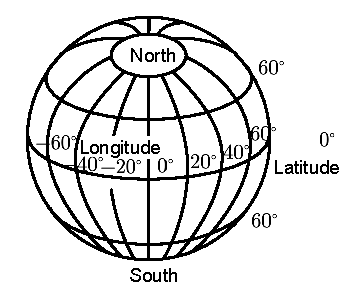
\includegraphics[width=0.4\textwidth]{ins/latlon.pdf}
	\caption{Schematic diagram of latitude-longitude coordinate system}
	\label{fig:latlon}
\end{figure}

The most common coordinate system on Earth is the \textbf{latitude-longitude} coordinate system, also known as the \textbf{Geographic Coordinate System} (see Figure~\ref{fig:latlon}). Combined with altitude, it forms the latitude-longitude-altitude (LLA) coordinate system. Latitude and longitude divide the Earth's surface uniformly: longitude ranges 180 degrees east and west from the prime meridian, while latitude ranges 90 degrees north and south from the equator. Both values are expressed in degrees or radians. Altitude can be either elevation above sea level or geodetic height relative to a reference surface.

While intuitive and globally applicable (being the default for many mapping systems), latitude-longitude coordinates become cumbersome for autonomous driving applications at city-scale or smaller areas. Building-level coordinates typically require 8-9 decimal places, and the nonlinear conversion to metric units (where 1 degree longitude corresponds to 0 meters at the poles but over 100 km at the equator) motivates the use of local coordinate systems.

\subsubsection{UTM Coordinate System}
The Universal Transverse Mercator (UTM) system projects the WGS84 ellipsoid Earth onto a transverse cylinder, divided into 60 longitudinal and 20 latitudinal zones with numeric and alphabetic labels respectively. While roughly uniform in angular distribution, metric distances vary due to Earth's curvature, with significant distortion excluding polar regions beyond 80° latitude.

Within each zone:
\begin{itemize}
	\item Easting coordinates reference a central meridian (assigned x=500,000m), increasing eastward
	\item Northing coordinates measure distance from the equator
	\item The resulting \textbf{ENU} (East-North-Up) system follows right-hand convention
	\item Alternative \textbf{NED} (North-East-Down) configurations also exist
\end{itemize}

UTM advantages include metric compatibility with sensors, though zone boundaries require special handling. Note:
\begin{enumerate}
	\item A 0.9996 scale factor corrects projection distortion
	\item ENU/NED systems have opposite Z-axis orientations affecting angle definitions
	\item Maximum easting span is ~667 km per zone
\end{enumerate}

This metric local frame facilitates autonomous vehicle operations while maintaining global reference.

\subsection{Display of RTK Measurements}
Many RTK and integrated navigation manufacturers can output coordinates in user-selected coordinate systems, with the most basic being the latitude-longitude coordinates measured by the RTK receiver. Below we demonstrate how to convert RTK's latitude-longitude coordinates to metric UTM coordinates while using a dual-antenna configuration to determine the vehicle's heading angle. Here we disregard the vehicle's pitch and roll, treating them as zero. Thus, although the vehicle outputs \textbf{4-DOF coordinates}, under the assumption of zero pitch and roll, the RTK output can also be considered as a 6-DOF pose transformation, i.e., an $\mathrm{SE}(3)$ pose.

We continue using the data from the previous section. This data consists of IMU, RTK, and wheel speed measurements located in the `data/ch3/` directory. Readers can open these files with a text editor, with the format as follows:

\begin{lstlisting}[language=sh, caption=Example data file]
	GNSS 1571900872.47168827 30.0011840411666668 117.97859182983332 305.98748779296875 
	330.047799999999995 1
	ODOM 1571900872.50085688 0 0
	IMU 1571900872.56527948 -0.000740019602845583204 -0.000471238898038460995 
	6.98131700797720067e-06 0.362519161666666645 -0.0608012299999999908 
	9.82135997500000002
\end{lstlisting}

Each line in the file represents a measurement, with the prefix "GNSS", "IMU", or "ODOM" indicating the record type. For GNSS measurements, each line contains: timestamp, latitude, longitude, altitude, heading angle, and heading validity flag. For IMU or wheel speed measurements, the readings from the accelerometer, gyroscope, and wheel speed sensors are provided. The GNSS positioning here is provided by the Qianxun FindCM solution, with a nominal accuracy of 2 cm in fixed solution mode.

Since the algorithm for converting latitude-longitude to UTM coordinates is complex and not the focus of this book, we use an open-source conversion method from the `thirdparty/utm_convert` directory\footnote{See: \url{https://github.com/hobu/mgrs}}. We've added a wrapper function to conveniently compute the $\mathrm{SE}(3)$ pose corresponding to GNSS measurements. The conversion code is as follows:

\begin{lstlisting}[language=c++,caption=ch3/utm\_convert.cc]
bool LatLon2UTM(const Vec2d& latlon, UTMCoordinate& utm_coor) {
	long zone = 0;
	char char_north = 0;
	long ret = Convert_Geodetic_To_UTM(latlon[0] * math::kDEG2RAD, latlon[1] * math::kDEG2RAD, &zone, &char_north,
	&utm_coor.xy_[0], &utm_coor.xy_[1]);
	utm_coor.zone_ = (int)zone;
	utm_coor.north_ = char_north == 'N';
	
	return ret == 0;
}

bool ConvertGps2UTM(GNSS& gps_msg, const Vec2d& antenna_pos, const double& antenna_angle, const Vec3d& map_origin) {
	/// Convert latitude-longitude-altitude to UTM
	UTMCoordinate utm_rtk;
	if (!LatLon2UTM(gps_msg.lat_lon_alt_.head<2>(), utm_rtk)) {
		return false;
	}
	utm_rtk.z_ = gps_msg.lat_lon_alt_[2];
	
	/// Convert GPS heading to radians
	double heading = 0;
	if (gps_msg.heading_valid_) {
		heading = (90 - gps_msg.heading_) * math::kDEG2RAD;  // Convert from NED to ENU
	}
	
	/// Transform from TWG to TWB
	SE3 TBG(SO3::rotZ(antenna_angle * math::kDEG2RAD), Vec3d(antenna_pos[0], antenna_pos[1], 0));
	SE3 TGB = TBG.inverse();
	
	/// Subtract map origin if specified
	double x = utm_rtk.xy_[0] - map_origin[0];
	double y = utm_rtk.xy_[1] - map_origin[1];
	double z = utm_rtk.z_ - map_origin[2];
	SE3 TWG(SO3::rotZ(heading), Vec3d(x, y, z));
	SE3 TWB = TWG * TGB;
	
	gps_msg.utm_valid_ = true;
	gps_msg.utm_.xy_[0] = TWB.translation().x();
	gps_msg.utm_.xy_[1] = TWB.translation().y();
	gps_msg.utm_.z_ = TWB.translation().z();
	
	if (gps_msg.heading_valid_) {
		// Construct pose with rotation
		gps_msg.utm_pose_ = TWB;
	} else {
		// Construct SE3 with only translation
		// Note: When installation offset exists, the actual vehicle pose cannot be derived
		gps_msg.utm_pose_ = SE3(SO3(), TWB.translation());
	}
	
	return true;
}
\end{lstlisting}

The latitude-longitude to UTM conversion is handled by the library function, while we need to transform the UTM coordinates from the GNSS frame to the vehicle's observed pose, considering the RTK's extrinsic parameters. The dual-antenna RTK installation used in this section is shown in Figure~\ref{fig:dual-rtk-coor}, where the blue axes $x_B, y_B, O_B$ represent the vehicle body frame, and the red axes $x_G, y_G, O_G$ represent the GNSS receiver frame.

Mathematically, we can treat the RTK's UTM coordinate reading as $\bm{T}_{WG}$, where $W$ represents the world frame and $G$ represents the GNSS receiver frame. To facilitate subsequent fusion localization, we transform it to $\bm{T}_{WB}$, where $B$ is the vehicle body frame. Thus, the extrinsic parameters between the GNSS receiver and the vehicle can be described by either $\bm{T}_{GB}$ or $\bm{T}_{BG}$.

\begin{figure}
	\centering
	\includegraphics[width=0.3\textwidth]{ins/dual-rtk-coor.pdf}
	\caption{RTK installation configuration used in this book's example. Subscript $G$ denotes the GNSS receiver frame, while $B$ denotes the vehicle body frame. The primary antenna is located at the right rear of the vehicle, and the secondary antenna at the front left.}
	\label{fig:dual-rtk-coor}
\end{figure}

In the calibration parameters, we specify the installation offset $\bm{a}_t$ as the vector from $O_B$ to $O_G$ expressed in the $B$ frame, which essentially corresponds to the translational component of $\bm{T}_{BG}$. Simultaneously, the installation angle $a_{\theta}$ is defined as the rotation angle from the $x$-axis of the $B$ frame to the $x$-axis of the $G$ frame. Substituting $\bm{a}_t$ and $a_{\theta}$ into $\bm{T}_{BG}$, we obtain:

\begin{equation}\label{key}
	\bm{T}_{BG} = \begin{bmatrix}
		\bm{R}_Z (a_{\theta}) & \bm{a}_t \\
		\bm{0}^\top & 1
	\end{bmatrix},
\end{equation}

where $\bm{R}_Z$ represents the rotation matrix about the $Z$-axis.

It's important to note that this definition of \textbf{installation angle} and \textbf{installation offset} is intuitive but not unique. The specific definition should prioritize operational convenience. These parameters could alternatively be defined in the opposite direction, as long as calibration personnel can measure them easily. We typically align mathematical notation with practical conventions rather than forcing real-world operations to conform to mathematical definitions. While calibration personnel might struggle to directly measure $\bm{R}_{BG}$ or $\bm{t}_{BG}$, they can easily measure the connection between two points or the angle between two lines.

The transformation matrix $\bm{T}_{WB}$ from the vehicle body frame to the world frame can be derived from RTK measurements and its extrinsic parameters:

\begin{equation}\label{key}
	\bm{T}_{WB} = \bm{T}_{WG} \bm{T}_{GB}.
\end{equation}

Expanding the rotation and translation components yields:

\begin{equation}\label{key}
	\bm{R}_{WB} = \bm{R}_{WG} \bm{R}_{GB}, \quad \bm{t}_{WB} = \bm{R}_{WG} \bm{t}_{GB} + \bm{t}_{WG}.
\end{equation}

An important consideration: even with known RTK extrinsic parameters $\bm{t}_{GB}$, determining the vehicle coordinates $\bm{t}_{WB}$ requires knowledge of the RTK orientation $\bm{R}_{WG}$. In a single-antenna configuration with non-zero installation offset $\bm{t}_{GB}$, \textbf{the vehicle's world coordinates cannot be precisely determined when the vehicle orientation is unknown}. However, in state estimation algorithms where the vehicle attitude $\bm{R}_{WB}$ is estimated, we can use $\bm{R}_{WB} \bm{R}_{BG}$ as the current $\bm{R}_{WG}$.

Additionally, the conversion program handles the transformation between \textbf{ENU} (East-North-Up) and \textbf{NED} (North-East-Down) coordinate systems. Different RTK manufacturers may output angles according to their predefined schemes, potentially causing inconsistencies in angle definitions. This book uses UTM coordinates with east and north as $XY$ axes (ENU frame), while the RTK manufacturer outputs NED coordinates. The former uses east as zero degrees, while the latter uses north as zero degrees with opposite rotation direction. Therefore, an azimuth angle $h$ in the NED frame converts to angle $h'$ in the ENU frame as:

\begin{equation}\label{key}
	h' = \pi/2 - h.
\end{equation}

The code above implements this angle conversion.

We then write a program to convert GNSS readings from the data file into poses and write them to an output file. Readers can use Python scripts to plot the entire GNSS trajectory. Simultaneously, we display the RTK poses in real-time graphical interfaces, allowing immediate visualization of current position and orientation.

\subsection{RTK Measurement Visualization}
Many RTK and integrated navigation manufacturers can output coordinates in user-selected coordinate systems, with the most basic output being the latitude-longitude coordinates measured by the RTK receiver. Below we demonstrate how to convert RTK's latitude-longitude coordinates to metric UTM coordinates while using a dual-antenna configuration to determine the vehicle's heading angle.

\begin{lstlisting}[language=c++,caption=ch3/process\_gnss.cc]
DEFINE_string(txt_path, "./data/ch3/10.txt", "Input data file path");

// Parameters specific to the provided dataset
DEFINE_double(antenna_angle, 12.06, "RTK antenna installation angle (degrees)");
DEFINE_double(antenna_pox_x, -0.17, "RTK antenna installation offset X");
DEFINE_double(antenna_pox_y, -0.20, "RTK antenna installation offset Y");

/**
* This program demonstrates GNSS data processing
* We convert raw GNSS readings into 6-DOF poses for subsequent processing
* Requires UTM conversion, RTK antenna extrinsics, and coordinate transformation
*
* Results are saved to file and visualized using Python scripts
*/

int main(int argc, char** argv) {
	sad::TxtIO io(fLS::FLAGS_txt_path);
	
	std::ofstream fout("./data/ch3/gnss_output.txt");
	Vec2d antenna_pos(FLAGS_antenna_pox_x, FLAGS_antenna_pox_y);
	
	auto save_result = [](std::ofstream& fout, double timestamp, const SE3& pose) {
		auto save_vec3 = [](std::ofstream& fout, const Vec3d& v) { 
			fout << v[0] << " " << v[1] << " " << v[2] << " "; 
		};
		auto save_quat = [](std::ofstream& fout, const Quatd& q) {
			fout << q.w() << " " << q.x() << " " << q.y() << " " << q.z() << " ";
		};
		
		fout << std::setprecision(18) << timestamp << " " << std::setprecision(9);
		save_vec3(fout, pose.translation());
		save_quat(fout, pose.unit_quaternion());
		fout << std::endl;
	};
	
	std::shared_ptr<sad::ui::PangolinWindow> ui = nullptr;
	if (FLAGS_with_ui) {
		ui = std::make_shared<sad::ui::PangolinWindow>();
		ui->Init();
	}
	
	bool first_gnss_set = false;
	Vec3d origin = Vec3d::Zero();
	io.SetGNSSProcessFunc([&](const sad::GNSS& gnss) {
		sad::GNSS gnss_out = gnss;
		if (sad::ConvertGps2UTM(gnss_out, antenna_pos, FLAGS_antenna_angle)) {
			if (first_gnss_set == false) {
				origin = gnss_out.utm_pose_.translation();
				first_gnss_set = true;
			}
			gnss_out.utm_pose_.translation() -= origin;
			
			save_result(fout, gnss_out.unix_time_, gnss_out.utm_pose_);
			ui->UpdateNavState(
			sad::NavStated(gnss_out.unix_time_, gnss_out.utm_pose_.so3(), 
			gnss_out.utm_pose_.translation()));
			
			usleep(1e4);
		}
	}).Go();
	
	if (ui) {
		while (!ui->ShouldQuit()) {
			usleep(1e5);
		}
		ui->Quit();
	}
	
	return 0;
}
\end{lstlisting}

The program converts RTK readings to UTM poses, removes the origin offset, writes to a text file, and displays in UI. To run:

\begin{lstlisting}[language=sh, caption=Terminal command:]
	bin/process_gnss --txt_path ./data/ch3/10.txt
\end{lstlisting}

The converted 6-DOF coordinates are saved in data/ch3/gnss_output.txt. Visualization scripts:

\begin{lstlisting}[language=sh, caption=Terminal command:]
	python3 scripts/plot_ch3_gnss_2d.py ./data/ch3/gnss_output.txt 
\end{lstlisting}

Figure~\ref{fig:gnss-traj} shows 2D and 3D trajectory plots. Observations:
\begin{itemize}
	\item RTK provides excellent horizontal trajectory accuracy
	\item Vertical measurements show noticeable noise and errors
	\item The example shows good GNSS conditions; other datasets include challenging segments
\end{itemize}

\begin{figure}
	\centering
	\includegraphics[width=1.0\textwidth]{ins/gnss-traj.pdf}
	\caption{2D and 3D views of GNSS trajectory}
	\label{fig:gnss-traj}
\end{figure}

The real-time display (Figure~\ref{fig:process-gnss}) shows:
\begin{itemize}
	\item Proper vehicle orientation (X-forward, Y-left, Z-up) when RTK heading is valid
	\item Noticeable instability in angle measurements compared to position
	\item Position jitter during heading outages due to incomplete pose solution
\end{itemize}

\begin{figure}
	\centering
	\includegraphics[width=1.0\textwidth]{ins/ch3-process-gnss.png}
	\caption{Real-time GNSS trajectory visualization}
	\label{fig:process-gnss}
\end{figure}

Note: This section only uses RTK-provided position and heading. Some RTK/INS systems output additional IMU data (angular/linear velocity), but we focus on fundamental principles here.

\section{Implementing Integrated Navigation Using Error-State Kalman Filter}
The RTK device provides us with a somewhat unstable pose observation source. We can directly treat it as an observation input for a positioning filter. In this section, we will combine RTK with IMU using an extended Kalman filter to form a traditional integrated navigation algorithm for subsequent algorithm comparisons. Strictly speaking, what we present to readers is the \textbf{Error-State Kalman Filter} (ESKF). The ESKF finds extensive applications ranging from GINS integrated navigation to visual SLAM\cite{Kleinert2010,Li2013,Davison2003} and extrinsic calibration\cite{Kelly2011,Mirzaei2008}. 

Why do we need ESKF? What's the difference between ESKF and EKF? We'll start from the motivation level. This progressive approach from simple to complex can also help readers better understand the development process of various algorithms.

\subsection{Mathematical Derivation of ESKF}
We have previously introduced the observation model of IMU devices. Now we need to treat IMU as the motion model and GNSS observations as the measurement model to derive the complete filter. This is not particularly difficult.

We define the state variables as:
\begin{equation}\label{key}
	\bm{x} = [\bm{p}, \bm{v}, \bm{R}, \bm{b}_g, \bm{b}_a, \bm{g}]^\top,
\end{equation}
where all variables default to subscript $()_{WB}$, with $\bm{p}$ representing translation, $\bm{v}$ velocity, $\bm{R}$ rotation, $\bm{b}_g, \bm{b}_a$ biases, and $\bm{g}$ gravity. According to the kinematic equations \eqref{eq:motion-equation} we introduced earlier and substituting IMU measurements, the continuous-time motion equations for the state variables are:
\begin{subequations}\label{eq:ekf-continous}
	\begin{align}
		\dot{\bm{p}} &= \bm{v}, \\
		\dot{\bm{v}} &= \bm{R} (\tilde{\bm{a}} - \bm{b}_{a} - \boldsymbol{\eta}_a) + \bm{g}, \\
		\dot{\bm{R}} &= \bm{R} \left( \tilde{\boldsymbol{\omega}} - \bm{b}_{g} - \boldsymbol{\eta}_g 
		\right)^\wedge, \\
		\dot{\bm{b}}_{g} & = \boldsymbol{\eta}_{bg}, \\
		\dot{\bm{b}}_{a} & = \boldsymbol{\eta}_{ba}, \\ 
		\dot{\bm{g}} &= \bm{0}.
	\end{align}
\end{subequations}

To predict the covariance in the EKF prediction step, we need to linearize these equations. Theoretically, the discrete-time linearized form is:
\begin{equation}\label{key}
	\bm{x}_{k+1} = \bm{f} (\bm{x}_k) + \bm{F} \mathrm{d} \bm{x} + \bm{w},
\end{equation}
where $\bm{F} = \left. \frac{\partial \bm{f}}{\partial \bm{x}} \right|_{\bm{x}_{k}}$ is the coefficient matrix. However, we encounter a practical problem: on one hand, $\bm{F}$ needs to compute the derivative of the rotation matrix $\bm{R}$ relative to some perturbation, and without introducing tensors, we cannot express the derivative of a matrix with respect to a vector. Traditional algorithms often compromise by using Euler angles or four scalars of quaternions as state variables\cite{crassidis2006sigma}, but this approach cannot elegantly utilize methods on manifolds. On the other hand, if we consider integrating inertial navigation systems with satellite navigation systems, the translation variables in $\bm{x}$ should use a global coordinate system. This makes the numerical values in $\bm{x}$ very large, potentially exceeding the effective digit range of floating-point numbers in some scenarios, leading to common computational failures like "large number swallowing small number" in numerical calculations\cite{bonnans2006numerical}.

This leads us to consider: can we avoid directly using $\bm{x}$ and $\bm{P}$ to express the mean and covariance of the state when deriving the motion and observation equations? Can we use the \textbf{update quantity} from the original Kalman filter to derive these two equations? Recall the observation part of the Kalman filter:
\begin{equation}\label{key}
	\bm{x}_k = \bm{x}_{k, \text{pred}} + \bm{K}_k \underbrace{(\bm{z}_k - \bm{H}_k \bm{x}_{k, \text{pred}})}_{\text{update quantity}}.
\end{equation}

In the context of manifolds, the update quantity on the right side should be a vector in the tangent space, and the addition in the middle should be the generalized addition of the manifold and the exponential map of the tangent space. However, we can also treat the update quantity (or error state) as the state variable of the filter to derive the motion and observation models. This leads to the \textbf{Error-State Kalman Filter}. Furthermore, not just for translation and rotation, we express all states in terms of error states, which is the typical approach of ESKF.

The ESKF is widely used in many traditional and modern systems, serving both as a filter for integrated navigation and for implementing complex systems like LIO and VIO\cite{Xu2021,xu2021fast, Bloesch2017}. Compared to traditional KF, the advantages of ESKF can be summarized as follows\cite{Madyastha2011}:
\begin{enumerate}
	\item In handling rotation, ESKF state variables can use minimal parameter representation, i.e., using three-dimensional variables to express rotation increments. These variables lie in the tangent space, which is a vector space. Traditional KF requires quaternions (4D) or higher-dimensional variables (rotation matrices, 9D) to express the state, or must use representations with singularities (Euler angles).
	\item ESKF always operates near the origin, far from singular points, making it more numerically stable and avoiding issues where linearization approximations become inadequate due to operating too far from the working point.
	\item The ESKF state quantities are small, making their second-order variables relatively negligible. Most Jacobian matrices become very simple under small quantities, sometimes even replaceable by identity matrices.
	\item The kinematics of error states are also smaller compared to the original state variables (kinematics of small quantities), allowing us to return the update part to the original state variables.
\end{enumerate}
In ESKF, we typically refer to the original state variables as \textbf{nominal state variables} and the state variables in ESKF as \textbf{error state variables}. The sum of nominal and error state variables is called the \textbf{true value}. By handling noise in the error state variables, we can consider the equations for nominal state variables as noise-free. This approach may seem complex initially, but separating the noise makes the nominal state equations more concise. The filter itself primarily needs to consider how the error state evolves, is observed, and finally filtered, with minimal relation to the nominal state.

The ESKF workflow is as follows: When IMU measurement data arrives, we integrate it into the nominal state variables. Since this approach doesn't account for noise, the results naturally drift quickly, so we treat the error component as error variables. During motion, the nominal state propagates with IMU data, while the error state grows due to Gaussian noise. At this point, the mean and covariance of ESKF's error state describe the specific magnitude of error state expansion (treated as a Gaussian distribution)\footnote{However, as we'll see later, since all noise terms are zero-mean white noise, the mean of the error state remains zero in the motion equations, only the covariance increases.}. Additionally, ESKF's update process relies on sensor observations beyond IMU. During updates, we use sensor data to update the \textbf{posterior} mean and covariance of the error state. We can then \textbf{merge} this error into the nominal state variables and reset ESKF to zero, completing one predict-update cycle.

Let's derive the two processes of ESKF. We define the true state of ESKF as: $\bm{x}_t = [\bm{p}_t, \bm{v}_t, \bm{R}_t, \bm{b}_{at}, \bm{b}_{gt}, \bm{g}_t]^\top$. The subscript $t$ denotes $\text{true}$, i.e., the true state. This state changes over time and can be denoted as $\bm{x}_t(t)$. In continuous time, we record IMU readings as $\tilde{\boldsymbol{\omega}}, \tilde{\bm{a}}$, allowing us to write the relationship between state variable derivatives and observations:

\begin{subequations}\label{eq:eskf-true-state}
	\begin{align}
		\dot{\bm{p}}_t &= \bm{v}_t, \\
		\dot{\bm{v}}_t &= \bm{R}_t (\tilde{\bm{a}} - \bm{b}_{at} - \boldsymbol{\eta}_a) + \bm{g}_t, \\
		\dot{\bm{R}}_t &= \bm{R}_t \left( \tilde{\boldsymbol{\omega}} - \bm{b}_{gt} - \boldsymbol{\eta}_g \right)^\wedge, \\
		\dot{\bm{b}}_{gt} &= \boldsymbol{\eta}_{bg}, \\
		\dot{\bm{b}}_{at} &= \boldsymbol{\eta}_{ba}, \\ 
		\dot{\bm{g}}_t &= \bm{0}.
	\end{align}
\end{subequations}

This is consistent with Equation \eqref{eq:ekf-continous} mentioned earlier. Note that including gravity $\bm{g}$ mainly facilitates determining the IMU's initial attitude. If we don't express gravity in the state equation, we must determine the IMU's initial orientation $\bm{R}(0)$ beforehand to perform subsequent calculations. In this case, the IMU's attitude is described relative to the initial horizontal plane. By explicitly expressing gravity, we can set the IMU's initial attitude as the identity matrix $\bm{R}=\bm{I}$, treating the gravity direction as a measure of the IMU's current attitude relative to the horizontal plane. Both methods are feasible, but separately expressing gravity makes initial attitude representation simpler and increases some linearity\cite{Lupton2009}.

If we organize observations and noise into a vector, we can express the above in matrix form. However, such a matrix would contain many zero entries without significant simplification over the current form, so we'll continue using these expanded equations. Next, we derive the error state equations. First, define the error state variables as:

\begin{subequations}\label{eq:eskf-true-to-error}
	\begin{align}
		\bm{p}_t &= \bm{p} + \delta \bm{p}, \\
		\bm{v}_t &= \bm{v} + \delta \bm{v}, \\
		\bm{R}_t &= \bm{R} \delta \bm{R} \quad \text{or} \ \bm{q}_t = \bm{q} \delta \bm{q}, \\
		\bm{b}_{gt} &= \bm{b}_g + \delta \bm{b}_g, \\
		\bm{b}_{at} &= \bm{b}_a + \delta \bm{b}_a, \\
		\bm{g}_t &= \bm{g} + \delta \bm{g}.
	\end{align}
\end{subequations}

The terms without subscripts are the \textbf{nominal state variables} in Equation (\ref{eq:eskf-true-state}). The kinematic equations for nominal state variables are identical to the true values, except they \textbf{ignore noise} (since noise is considered in the error state equations). For the rotation part, $\delta \bm{R}$ can be represented by its Lie algebra $\mathrm{Exp}(\delta \boldsymbol{\theta})$, requiring Equation (c) to be expressed in exponential form.

For error state Equations (a,d,e,f), taking time derivatives on both sides easily yields corresponding derivative expressions:

\begin{subequations}
	\begin{align}
		\delta \dot{\bm{p}} &= \delta \bm{v}, \\
		\delta \dot{\bm{b}_g} &= \boldsymbol{\eta}_{bg}, \\
		\delta \dot{\bm{b}_a} &= \boldsymbol{\eta}_{ba}, \\
		\delta \dot{\bm{g}} &= \bm{0}.
	\end{align}
\end{subequations}

Equations (b) and (c) are slightly more complex due to their relationship with $\delta \bm{R}$, and we provide their separate derivation below.

\subsubsection{Error State Rotation Term}
Taking the time derivative of both sides of Equation (\ref{eq:eskf-true-to-error})(c) yields:

\begin{equation}\label{eq:eskf-3.19}
	\begin{aligned}
		\dot{\bm{R}}_t &= \dot{\bm{R}} \mathrm{Exp} (\delta \boldsymbol{\theta}) + \bm{R} 
		\dot{\mathrm{Exp}(\delta \boldsymbol{\theta})},  \\
		&\buildrel{\ref{eq:eskf-true-state}(c)}\over=  \bm{R}_t \left( \tilde{\boldsymbol{\omega}} - 
		\bm{b}_{gt} - \boldsymbol{\eta}_g \right) ^\wedge.
	\end{aligned}
\end{equation}

Note that the term $\dot{\mathrm{Exp}(\delta \boldsymbol{\theta})}$ on the right side satisfies:
\begin{equation}
	\dot{\mathrm{Exp}(\delta \boldsymbol{\theta})} = \mathrm{Exp}(\delta \boldsymbol{\theta}) \delta 
	\dot{\boldsymbol{\theta}}^\wedge.
\end{equation} 

Thus, the first expression in \eqref{eq:eskf-3.19} can be written as:
\begin{equation}\label{key}
	\dot{\bm{R}} \mathrm{Exp} (\delta \boldsymbol{\theta}) + \bm{R} \dot{\mathrm{Exp}(\delta 
		\boldsymbol{\theta})} = \bm{R} (\tilde{\boldsymbol{\omega}}-\bm{b}_g)^\wedge 
	\mathrm{Exp}(\delta \boldsymbol{\theta}) + \bm{R} \mathrm{Exp}(\delta \boldsymbol{\theta} ) 
	\delta \dot{\boldsymbol{\theta}}^\wedge.
\end{equation}

While the second expression becomes:
\begin{equation}\label{key}
	\begin{aligned}
		\bm{R}_t \left( \tilde{\boldsymbol{\omega}} - \bm{b}_{gt} - \boldsymbol{\eta}_g \right)^\wedge 
		&= \bm{R}  \mathrm{Exp} (\delta \boldsymbol{\theta}) \left( \tilde{\boldsymbol{\omega}} - 
		\bm{b}_{gt} - \boldsymbol{\eta}_g \right)^\wedge.
	\end{aligned}
\end{equation}

By comparing these two expressions, moving $\delta \dot{\boldsymbol{\theta}}^\wedge$ to one side, canceling $\bm{R}$ on both sides, and organizing similar terms, we obtain:
\begin{equation}
	\begin{aligned}
		\mathrm{Exp} (\delta \boldsymbol{\theta}) \delta \dot{\boldsymbol{\theta}}^\wedge &= 
		\mathrm{Exp} (\delta \boldsymbol{\theta}) \left( \tilde{\boldsymbol{\omega}} - \bm{b}_{gt} - 
		\boldsymbol{\eta}_g \right)^\wedge - (\tilde{\boldsymbol{\omega}}-\bm{b}_g)^\wedge 
		\mathrm{Exp}(\delta \boldsymbol{\theta}).
	\end{aligned}
\end{equation}

Noting that $\mathrm{Exp}(\delta \boldsymbol{\theta})$ itself is an $\mathrm{SO}(3)$ matrix, we utilize the adjoint property of $\mathrm{SO}(3)$:
\begin{equation}\label{key}
	\boldsymbol{\phi}^\wedge \bm{R} = \bm{R} (\bm{R}^\top \boldsymbol{\phi})^\wedge
\end{equation}
to interchange $\mathrm{Exp}(\delta \boldsymbol{\theta})$ above:
\begin{equation}\label{key}
	\begin{aligned}
		\mathrm{Exp} (\delta \boldsymbol{\theta}) \delta \dot{\boldsymbol{\theta}}^\wedge &= 
		\mathrm{Exp} (\delta \boldsymbol{\theta}) \left( \tilde{\boldsymbol{\omega}} - \bm{b}_{gt} - 
		\boldsymbol{\eta}_g \right)^\wedge - \mathrm{Exp} (\delta \boldsymbol{\theta})  \left( 
		\mathrm{Exp} (-\delta \boldsymbol{\theta})  (\tilde{\boldsymbol{\omega}}-\bm{b}_g) 
		\right)^\wedge \\
		&=  \mathrm{Exp} (\delta \boldsymbol{\theta}) \left[ (\tilde{\boldsymbol{\omega}} - \bm{b}_{gt} - 
		\boldsymbol{\eta}_g)^\wedge - (\mathrm{Exp} (-\delta \boldsymbol{\theta})  
		(\tilde{\boldsymbol{\omega}}-\bm{b}_g) )^\wedge \right] \\
		&\approx \mathrm{Exp} (\delta \boldsymbol{\theta}) \left[ (\tilde{\boldsymbol{\omega}} - 
		\bm{b}_{gt} - \boldsymbol{\eta}_g)^\wedge - \left((\bm{I} - \delta 
		\boldsymbol{\theta}^\wedge)(\tilde{\boldsymbol{\omega}}-\bm{b}_g )\right)^\wedge \right] \\
		&=  \mathrm{Exp} (\delta \boldsymbol{\theta}) \left[ \bm{b}_g - \bm{b}_{gt} -\boldsymbol{\eta}_g 
		+ \delta \boldsymbol{\theta}^\wedge \tilde{\boldsymbol{\omega}} - \delta 
		\boldsymbol{\theta}^\wedge \bm{b}_{g} \right]^\wedge \\
		&= \mathrm{Exp} (\delta \boldsymbol{\theta}) \left[ 
		(-\tilde{\boldsymbol{\omega}}+\bm{b}_g)^\wedge \delta \boldsymbol{\theta} - \delta \bm{b}_g - 
		\boldsymbol{\eta}_g \right]^\wedge.
	\end{aligned}
\end{equation}

After canceling the coefficients on the left side, we get:
\begin{equation}\label{key}
	\delta \dot{\boldsymbol{\theta}} \approx -(\tilde{\boldsymbol{\omega}} - \bm{b}_g)^\wedge \delta 
	\boldsymbol{\theta} - \delta \bm{b}_g - \boldsymbol{\eta}_g. 
\end{equation}

The $\approx$ in this equation comes from the expansion of $\mathrm{Exp}(-\delta \boldsymbol{\theta})$. If we ignore second-order small quantities of $\delta \boldsymbol{\theta}$, the equation can also be written with an equality sign.

\subsubsection{Velocity Term of the Error State}
Next, we consider the error form of Equation (\ref{eq:eskf-true-to-error})(b). Similarly, by taking the time derivative of both sides, we can obtain the expression for $\delta \dot{\bm{v}}$. The left-hand side of the equation is:
\begin{equation}
	\begin{aligned}
		\dot{\bm{v}}_t &= \bm{R}_t(\tilde{\bm{a}} - \bm{b}_{at} - \boldsymbol{\eta}_a) + \bm{g}_t \\
		&= \bm{R} \mathrm{Exp}(\delta \boldsymbol{\theta}) (\tilde{\bm{a}} - \bm{b}_a - \delta \bm{b}_a 
		- \boldsymbol{\eta}_a ) + \bm{g} + \delta \bm{g} \\
		&\approx \bm{R} (\bm{I} + \delta \boldsymbol{\theta}^\wedge ) (\tilde{\bm{a}} - \bm{b}_a - \delta 
		\bm{b}_a - \boldsymbol{\eta}_a) + \bm{g} + \delta \bm{g} \\
		&\approx \bm{R} \tilde{\bm{a}} - \bm{R} \bm{b}_a - \bm{R} \delta \bm{b}_a - \bm{R} 
		\boldsymbol{\eta}_a + \bm{R} \delta \boldsymbol{\theta}^\wedge \tilde{\bm{a}} - \bm{R} \delta 
		\boldsymbol{\theta}^\wedge \bm{b}_a + \bm{g} + \delta \bm{g} \\
		&= \bm{R} \tilde{\bm{a}} - \bm{R} \bm{b}_a - \bm{R} \delta \bm{b}_a - \bm{R} 
		\boldsymbol{\eta}_a - \bm{R} \tilde{\bm{a}}^\wedge \delta \boldsymbol{\theta}  + \bm{R} 
		\bm{b}_a^\wedge  \delta\boldsymbol{\theta}  + \bm{g} + \delta \bm{g}.
	\end{aligned}
\end{equation}
When moving from the third line to the fourth line, it is necessary to neglect the second-order small quantities resulting from the multiplication of $\delta \boldsymbol{\theta}^\wedge$ with $\delta \bm{b}_a$ and $\boldsymbol{\eta}_a$. The transition from the fourth line to the fifth line utilizes the property that the cross-product symbol changes sign when the order is swapped. On the other hand, the right-hand side of the equation is:

\begin{equation}\label{key}
	\dot{\bm{v}} + \delta \dot{\bm{v}} = \bm{R}(\tilde{\bm{a}} - \bm{b}_a) + \bm{g} + \delta \dot{\bm{v}}.
\end{equation}

Since the two expressions above are equal, we obtain:
\begin{equation}\label{key}
	\delta \dot{\bm{v}} = - \bm{R}(\tilde{\bm{a}} - \bm{b}_a)^\wedge \delta \boldsymbol{\theta} - 
	\bm{R} \delta \bm{b}_a  - \bm{R} \boldsymbol{\eta}_a + \delta \bm{g}.
\end{equation}

Thus, we have derived the kinematic model for $\delta \bm{v}$. It is worth noting that since $\boldsymbol{\eta}_a$ is a zero-mean white noise, multiplying it by any rotation matrix still results in a zero-mean white noise. Moreover, because $\bm{R}^\top \bm{R} = \bm{I}$, it is straightforward to show that its covariance matrix remains unchanged (left as an exercise). Therefore, the above equation can also be simplified as:
\begin{equation}\label{key}
	\delta \dot{\bm{v}} = - \bm{R}(\tilde{\bm{a}} - \bm{b}_a)^\wedge \delta \boldsymbol{\theta} - 
	\bm{R} \delta \bm{b}_a  - \boldsymbol{\eta}_a + \delta \bm{g}.
\end{equation}

At this point, we can summarize the kinematic equations for the error variables as follows:
\begin{subequations}\label{eq:eskf-error-state-continuous-time}
	\begin{align}
		\delta \dot{\bm{p}} &= \delta \bm{v}, \\
		\delta \dot{\bm{v}} &= - \bm{R}(\tilde{\bm{a}} - \bm{b}_a)^\wedge \delta \boldsymbol{\theta} - 
		\bm{R} \delta \bm{b}_a  - \boldsymbol{\eta}_a + \delta \bm{g}, \\
		\delta \dot{\boldsymbol{\theta}} &= -(\tilde{\boldsymbol{\omega}} - \bm{b}_g)^\wedge \delta 
		\boldsymbol{\theta} - \delta \bm{b}_g - \boldsymbol{\eta}_g, \\
		\delta \dot{\bm{b}_g} &= \boldsymbol{\eta}_{bg}, \\
		\delta \dot{\bm{b}_a} &= \boldsymbol{\eta}_{ba}, \\
		\delta \dot{\bm{g}} &= \bm{0} .
	\end{align}
\end{subequations}
\subsection{Discrete-Time ESKF Kinematic Equations}  
Deriving the discrete-time state equations from the continuous-time state equations is straightforward. Let us directly present them. The discrete-time kinematic equations for the \textbf{nominal state variables} can be written as:  
\begin{subequations}\label{key}  
	\begin{align}  
		\bm{p}(t+\Delta t) &= \bm{p}(t) + \bm{v} \Delta t + \frac{1}{2}   
		\left(\bm{R}(\tilde{\bm{a}}-\bm{b}_a) \right) \Delta t^2 + \frac{1}{2} \bm{g} \Delta t^2, \\  
		\bm{v}(t+\Delta t) &= \bm{v}(t) + \bm{R} (\tilde{\bm{a}} - \bm{b}_a) \Delta t + \bm{g} \Delta t,	\\  
		\bm{R}(t+\Delta t) &= \bm{R}(t) \mathrm{Exp} \left( (\tilde{\boldsymbol{\omega}}-\bm{b}_g)   
		\Delta t \right),\\  
		\bm{b}_g(t+\Delta t) &= \bm{b}_g(t), \\  
		\bm{b}_a(t+\Delta t) &= \bm{b}_a(t), \\  
		\bm{g}(t+\Delta t) &= \bm{g}(t) .  
	\end{align}  
\end{subequations}  
This equation is obtained by simply adding the bias terms and gravity term to Equation \eqref{eq:3.14}. Note that the third line is essentially the integration formula for angular velocity. The discrete form of the \textbf{error state} is very similar to that of the \textbf{nominal state}, but special attention must be paid to the angular velocity part:  

\begin{subequations}\label{eq:eskf-motion-equation}  
	\begin{align}  
		\delta \bm{p}(t+\Delta t) &= \delta \bm{p} + \delta \bm{v} \Delta t, \\  
		\delta \bm{v}(t+\Delta t) &= \delta \bm{v} + \left( - \bm{R}(\tilde{\bm{a}} - \bm{b}_a)^\wedge   
		\delta \boldsymbol{\theta} - \bm{R} \delta \bm{b}_a  + \delta \bm{g} \right) \Delta t -  
		\boldsymbol{\eta}_{v}, \\  
		\delta \boldsymbol{\theta} (t+\Delta t) &= \mathrm{Exp}\left( -(\tilde{\boldsymbol{\omega}} -   
		\bm{b}_g) \Delta t \right) \delta \boldsymbol{\theta} - \delta \bm{b}_g \Delta t -   
		\boldsymbol{\eta}_{\theta}, \\  
		\delta \bm{b}_g (t+\Delta t) &= \delta \bm{b}_g + \boldsymbol{\eta}_{bg}, \\  
		\delta \bm{b}_a (t+\Delta t)&= \delta \bm{b}_a + \boldsymbol{\eta}_{ba}, \\  
		\delta \bm{g} (t+\Delta t) &= \delta \bm{g}.  
	\end{align}  
\end{subequations}  

Notes:  
\begin{enumerate}  
	\item For simplicity, we omit the $(t)$ in parentheses on the right-hand side of the equations.  
	\item For the integration of the rotation part, we can treat Equation \eqref{eq:eskf-error-state-continuous-time}(c) as a differential equation for $\delta \boldsymbol{\theta}$ and solve it. The solution process is similar to integrating angular velocity.  
	\item The noise terms do not participate in the recursion and must be treated separately as part of the noise. Continuous-time noise terms can be regarded as the power spectral density of a random process, while discrete-time noise variables are the random variables we commonly encounter. The standard deviations of these noise random variables can be written as follows:  
	\begin{equation}\label{key}  
		\sigma(\boldsymbol{\eta}_v) = \Delta t \sigma_a(k), \quad \sigma(\boldsymbol{\eta}_{\theta}) =   
		\Delta t \sigma_{g}(k), \quad \sigma(\boldsymbol{\eta}_{bg}) = \sqrt{\Delta t} \sigma_{bg}, \quad   
		\sigma(\boldsymbol{\eta}_{ba}) = \sqrt{\Delta t} \sigma_{ba},  
	\end{equation}  
	where the $\Delta t$ in the first two equations arises from the integration relationship, and the last two equations are consistent with \eqref{eq:imu-noise-relationship}.  
\end{enumerate}  

At this point, we have described the process of IMU propagation in the ESKF, corresponding to the state equation in the Kalman filter. To ensure the convergence of the filter, external observations are needed to correct the Kalman filter, which is the so-called integrated navigation. Of course, there are many methods for integrated navigation, ranging from traditional EKF to the ESKF introduced in this section, as well as the pre-integration and graph optimization techniques to be discussed in later chapters, all of which can be applied to integrated navigation \cite{Wen2021}. In this section, we take the fusion of GNSS observations as an example to demonstrate how to integrate these observation data into the ESKF to form a convergent Kalman filter. In the application chapters at the end of this book, we will also introduce filter solutions that fuse LiDAR point clouds or LiDAR positioning data.
\subsection{Motion Process of ESKF}
Based on the above discussion, we can formulate the motion process of ESKF. The discrete-time motion equation for the error state variable $\delta \bm{x}$ has been given in Eq. \eqref{eq:eskf-motion-equation}, which can be expressed as:
\begin{equation}\label{eq:eskf-motion-process}
	\delta \bm{x}_{k+1} = \bm{f} (\delta \bm{x}_{k}) + \bm{w}, \quad \bm{w} \sim \mathcal{N}(\bm{0}, \bm{Q}),
\end{equation}
where $\bm{w}$ is the noise term. According to the previous definition, the noise covariance matrix $\bm{Q}$ should be:
\begin{equation}\label{eq:eskf-Q-matrix}
	\bm{Q} = \mathrm{diag}\left(\bm{0}_3, \mathrm{Cov}(\boldsymbol{\eta}_v), \mathrm{Cov}(\boldsymbol{\eta}_{\theta}), \mathrm{Cov}(\boldsymbol{\eta}_{bg}), \mathrm{Cov}(\boldsymbol{\eta}_{ba}), \bm{0}_3\right),
\end{equation}
where the zero matrices at the beginning and end are due to the fact that the position and gravity error equations themselves contain no noise.

To maintain consistency with EKF notation, we compute the linearized form of the motion equation:
\begin{equation}\label{eq:eskf-linearized}
	\delta \bm{x}(t+\Delta t) = \underbrace{\bm{f}(\delta \bm{x}(t))}_{=\bm{0}} + \bm{F} \delta \bm{x} + \bm{w},
\end{equation}
where $\bm{F}$ is the state transition Jacobian matrix. Since Eq. \eqref{eq:eskf-motion-equation} is already explicitly linearized, we can directly extract the coefficient matrix (note the variable order):
\begin{equation}\label{eq:eskf-F-matrix}
	\bm{F} = \begin{bmatrix}
		\bm{I} & \bm{I} \Delta t & \bm{0} & \bm{0} & \bm{0} & \bm{0} \\
		\bm{0} & \bm{I} & - \bm{R}(\tilde{\bm{a}} - \bm{b}_a)^\wedge \Delta t & \bm{0} & -\bm{R} \Delta t & \bm{I} \Delta t \\
		\bm{0} & \bm{0} & \mathrm{Exp}\left( -(\tilde{\boldsymbol{\omega}} - \bm{b}_g) \Delta t \right) &  -\bm{I} \Delta t & \bm{0} & \bm{0} \\
		\bm{0} & \bm{0} & \bm{0} & \bm{I} & \bm{0} & \bm{0} \\
		\bm{0} & \bm{0} & \bm{0} & \bm{0} & \bm{I} & \bm{0} \\
		\bm{0} & \bm{0} & \bm{0} & \bm{0} & \bm{0} & \bm{I} 
	\end{bmatrix}.
\end{equation}

On this basis, we implement the prediction process of ESKF. The prediction process includes:
\begin{itemize}
	\item Prediction of the nominal state (IMU integration)
	\item Prediction of the error state
\end{itemize}
\begin{subequations}\label{eq:motion-eskf}
	\begin{align}
		\delta \bm{x}_{\mathrm{pred}} &= \bm{F} \delta \bm{x}, \\
		\bm{P}_{\mathrm{pred}} &= \bm{F} \bm{P} \bm{F}^\top + \bm{Q}.
	\end{align}
\end{subequations}

However, since the error state of ESKF is reset to $\delta \bm{x} = \bm{0}$ after each update, the mean part of the motion equation (i.e., Eq. \eqref{eq:motion-eskf}(a)) is not particularly meaningful. The covariance part describes the distribution of the entire error estimate. Intuitively, the noise covariance $\bm{Q}$ added in the motion equation can be interpreted as an \textbf{increase} in uncertainty during the prediction process.

\subsection{Update Process of ESKF}
\label{subsec:3.4.4}
The previous section described the motion process of ESKF. Now we consider the update process. Assuming an abstract sensor can generate observations of the state variables with an observation equation $\bm{h}$, we can write:

\begin{equation}\label{eq:observation-model}
	\bm{z} = \bm{h}(\bm{x}) + \bm{v}, \quad \bm{v} \sim \mathcal{N}(\bm{0}, \bm{V}),
\end{equation}
where $\bm{z}$ is the observation data, $\bm{v}$ is the observation noise, and $\bm{V}$ is the noise covariance matrix\footnote{We use a different symbol here since $\bm{R}$ is already used in the state variables.}.

In traditional EKF, we can directly linearize the observation equation to compute the Jacobian matrix of the observation equation with respect to the state variables, then update the Kalman filter. In ESKF, since we have estimates of both the nominal state $\bm{x}$ and the error state $\delta \bm{x}$, and we want to update the error state, we need to compute the Jacobian matrix of the observation equation with respect to the error state:

\begin{equation}\label{eq:H-definition}
	\bm{H} = \left. \frac{\partial \bm{h}}{\partial \delta \bm{x}} \right|_{\bm{x}_{\text{pred}}},
\end{equation}

We then compute the Kalman gain and perform the error state update:

\begin{subequations}\label{eq:eskf-update}
	\begin{align}
		\bm{K} &= \bm{P}_{\mathrm{pred}} \bm{H}^\top(\bm{H} \bm{P}_{\mathrm{pred}} \bm{H}^\top + \bm{V})^{-1}, \\
		\delta \bm{x} &= \bm{K} (\bm{z} - \bm{h}(\bm{x}_{\mathrm{pred}})), \\
		\bm{x} &= \bm{x}_{\text{pred}} + \delta \bm{x}, \\
		\bm{P} &= (\bm{I} - \bm{K} \bm{H}) \bm{P}_{\mathrm{pred}}.
	\end{align}
\end{subequations}

Here $\bm{K}$ is the Kalman gain, $\bm{P}_{\mathrm{pred}}$ is the predicted covariance matrix, and $\bm{P}$ is the updated covariance matrix.

Most observation data are measurements of the nominal state\footnote{However, in some cases we can directly derive observations of the error state, which would simplify the subsequent derivation. Both GNSS and LiDAR observations discussed later will use direct observation of error states.}. In this case, $\bm{H}$ can be computed using the chain rule:

\begin{equation}\label{eq:H-chain-rule}
	\bm{H} = \frac{\partial \bm{h}}{\partial \bm{x}} \frac{\partial \bm{x}}{\partial \delta \bm{x}},
\end{equation}

The first term requires linearization of the observation equation. For the second term, based on our definition of state variables, we obtain:

\begin{equation}\label{eq:state-derivative}
	\frac{\partial \bm{x}}{\partial \delta \bm{x}} = \mathrm{diag}\left(\bm{I}_3, \bm{I}_3, \frac{\partial \mathrm{Log} (\bm{R}(\mathrm{Exp}(\delta \boldsymbol{\theta})))}{\partial \delta \boldsymbol{\theta}}, \bm{I}_3, \bm{I}_3, \bm{I}_3\right).
\end{equation}

While other terms are straightforward, the rotation part requires special attention since $\delta \boldsymbol{\theta}$ is defined as right multiplication of $\bm{R}$. Using the right BCH formula:

\begin{equation}\label{eq:rotation-derivative}
	\frac{\partial \mathrm{Log} (\bm{R}(\mathrm{Exp}(\delta \boldsymbol{\theta})))}{\partial \delta \boldsymbol{\theta}} = \bm{J}_r^{-1} (\bm{R}).
\end{equation}

Finally, we could add subscript $k$ to each variable to indicate the time step, but this is unnecessary as the above equations already clearly express their meanings. These formulas can also be derived using quaternion representation, with similar forms but more complex details (see \cite{Sola2017}). This book presents only the derivation using $\mathrm{SO}(3)$ and its Lie algebra.
\subsection{Post-Processing of ESKF Error State}
After completing the prediction and update processes, we have corrected the estimation of the error state. The next step is to incorporate the error state into the nominal state and then reset the ESKF. The incorporation can be simply expressed as:

\begin{subequations}\label{eq:error-state-incorporation}
	\begin{align}
		\bm{p}_{k+1} &= \bm{p}_k + \delta \bm{p}_k, \\
		\bm{v}_{k+1} &= \bm{v}_k + \delta \bm{v}_k, \\
		\bm{R}_{k+1} &= \bm{R}_k \mathrm{Exp}(\delta \boldsymbol{\theta}_k), \\
		\bm{b}_{g, k+1} &= \bm{b}_{g,k} + \delta \bm{b}_{g,k}, \\
		\bm{b}_{a, k+1} &= \bm{b}_{a,k} + \delta \bm{b}_{a,k}, \\
		\bm{g}_{k+1} &= \bm{g}_{k} + \delta \bm{g}_{k}.
	\end{align}
\end{subequations}

Some literature defines this computation as a generalized state variable addition operation:
\begin{equation}\label{eq:generalized-addition}
	\bm{x}_{k+1} = \bm{x}_k \oplus \delta \bm{x}_{k},
\end{equation}
This notation can simplify the overall expression but sacrifices some readability. When formulas contain too many generalized addition/subtraction operations (especially different definitions like $\oplus$, $\boxplus$, $\ominus$, $\boxminus$, etc.), it becomes difficult for readers to quickly recognize their specific meanings. Therefore, this book prefers to explicitly write out each state component using standard addition rather than generalized addition symbols.

The ESKF reset consists of two parts: mean reset and covariance reset. The mean part can be simply implemented as:
\begin{equation}\label{eq:mean-reset}
	\delta \bm{x} = \bm{0}.
\end{equation}

Since the mean has been reset, the covariance we previously described was in the tangent space of $\bm{x}_k$, but now needs to describe the covariance in $\bm{x}_{k+1}$. This reset introduces some subtle differences, primarily affecting the rotation component. In fact, before resetting, the Kalman filter characterized a Gaussian distribution $\mathcal{N}(\delta \bm{x}, \bm{P})$ in the tangent space of $\bm{x}_{\mathrm{pred}}$, while after resetting, it should characterize $\mathcal{N}(0, \bm{P}_{\mathrm{reset}})$ at $\bm{x}_{\mathrm{pred}} + \delta \bm{x}$. This is identical for vector states, but for rotation variables, the zero point of their tangent space has changed, requiring mathematical distinction.

Let the nominal rotation estimate before reset be $\bm{R}_k$, the error state be $\delta \boldsymbol{\theta}$, and the Kalman filter's incremental result be $\delta \boldsymbol{\theta}_k$\footnote{Note that here $\delta \boldsymbol{\theta}_k$ is known, while $\delta \boldsymbol{\theta}$ is a random variable.}. After reset, the nominal rotation becomes $\bm{R}_k \mathrm{Exp}(\delta \boldsymbol{\theta}_k)=\bm{R}^+$, and the error state becomes $\delta \boldsymbol{\theta}^+$. Since the error state is reset, clearly $\delta \boldsymbol{\theta}^+ = \bm{0}$. However, what we care about is not their direct values but the linearized relationship between $\delta \boldsymbol{\theta}^+$ and $\delta \boldsymbol{\theta}$. Writing out the actual reset process:

\begin{equation}\label{eq:reset-process}
	\bm{R}^+ \mathrm{Exp}(\delta \boldsymbol{\theta}^+) = \bm{R}_k \mathrm{Exp}(\delta \boldsymbol{\theta}_k) \mathrm{Exp}(\delta \boldsymbol{\theta}^+) = \bm{R}_k \mathrm{Exp}(\delta \boldsymbol{\theta}).
\end{equation}

We can obtain:
\begin{equation}\label{eq:reset-relation}
	\mathrm{Exp}(\delta \boldsymbol{\theta}^+) = \mathrm{Exp}(-\delta \boldsymbol{\theta}_k) \mathrm{Exp}(\delta \boldsymbol{\theta}),
\end{equation}

Here $\delta \boldsymbol{\theta}$ is small. Using the linearized BCH formula, we get:
\begin{equation}\label{eq:linearized-reset}
	\delta \boldsymbol{\theta}^+ = -\delta \boldsymbol{\theta}_k + \delta \boldsymbol{\theta} - \frac{1}{2} \delta \boldsymbol{\theta}_k^\wedge \delta \boldsymbol{\theta} + o((\delta \boldsymbol{\theta})^2) .
\end{equation}

Thus:
\begin{equation}\label{eq:jacobian-derivation}
	\frac{\partial \delta \boldsymbol{\theta}^+}{\partial \delta \boldsymbol{\theta}} \approx \bm{I} - \frac{1}{2} \delta \boldsymbol{\theta}_k^\wedge .
\end{equation}

This shows that the error states before and after reset differ by a small Jacobian matrix in rotation, which we denote as $\bm{J}_{\boldsymbol{\theta}} = \bm{I} - \frac{1}{2} \delta \boldsymbol{\theta}_k^\wedge $. Extending this small Jacobian to the full state dimension while keeping other parts as identity matrices gives the complete Jacobian:

\begin{equation}\label{eq:full-jacobian}
	\bm{J}_k = \mathrm{diag}(\bm{I}_3, \bm{I}_3, \bm{J}_{\boldsymbol{\theta}}, \bm{I}_3, \bm{I}_3, \bm{I}_3),
\end{equation}

Therefore, while resetting the error state mean to zero, their covariance matrix should also undergo linear transformation:
\begin{equation}\label{eq:tangent-space-projection}
	\bm{P}_{\mathrm{reset}} = \bm{J}_k \bm{P} \bm{J}_k^\top.
\end{equation}

However, since $\delta \boldsymbol{\theta}_k$ is not large, $\bm{J}_k$ remains very close to the identity matrix. Therefore, most materials do not handle this term but directly use the previously estimated $\bm{P}$ matrix as the starting point for the next time step. Nevertheless, this book still introduces this concept and will further discuss it in Chapter~\ref{cpt:tightly-lio}. The practical significance of this issue is performing a \textbf{tangent space projection}, i.e., projecting a Gaussian distribution from one tangent space to another. In ESKF, the difference is not significant, but the later Iterated Extended Kalman Filter (IESKF) will involve multiple tangent space transformations during the observation process. In comparison, ESKF only has a single transformation during reset, making its principle simpler.
\section{Implementation of ESKF-based Integrated Navigation}

Below we implement an ESKF that fuses IMU and GNSS observations. The code in this section will output results to text files for subsequent visualization. During the ESKF implementation, we will encounter some practical details that will be discussed here.

\subsection{Implementation of the ESKF Filter}

First, we define the ESKF class. Its member variables should include the nominal state, error state, covariance matrix, and various sensor noise parameters.

\begin{lstlisting}[language=c++,caption=src/ch3/eskf.hpp]
template <typename S = double>
class ESKF {
	/// Type definitions
	using SO3 = Sophus::SO3<S>;                     // Rotation type
	using VecT = Eigen::Matrix<S, 3, 1>;            // Vector type
	using Vec18T = Eigen::Matrix<S, 18, 1>;         // 18-dimensional vector
	using Mat3T = Eigen::Matrix<S, 3, 3>;           // 3x3 matrix
	using MotionNoiseT = Eigen::Matrix<S, 18, 18>;  // Motion noise type
	using OdomNoiseT = Eigen::Matrix<S, 3, 3>;      // Odometry noise type
	using GnssNoiseT = Eigen::Matrix<S, 6, 6>;      // GNSS noise type
	using Mat18T = Eigen::Matrix<S, 18, 18>;        // 18-dimensional covariance
	using NavStateT = NavState<S>;                  // Complete nominal state type
	
	/// Other constructors and member functions omitted
	private:
	/// Member variables
	double current_time_ = 0.0;  // Current timestamp
	
	/// Nominal state
	VecT p_ = VecT::Zero();
	VecT v_ = VecT::Zero();
	SO3 R_;
	VecT bg_ = VecT::Zero();
	VecT ba_ = VecT::Zero();
	VecT g_{0, 0, -9.8};
	
	/// Error state
	Vec18T dx_ = Vec18T::Zero();
	
	/// Covariance matrix
	Mat18T cov_ = Mat18T::Identity();
	
	/// Noise matrices
	MotionNoiseT Q_ = MotionNoiseT::Zero();
	OdomNoiseT odom_noise_ = OdomNoiseT::Zero();
	GnssNoiseT gnss_noise_ = GnssNoiseT::Zero();
	
	/// Flags
	bool first_gnss_ = true;  // Whether it's the first GNSS data
	
	/// Configuration options
	Options options_;
};

using ESKFD = ESKF<double>;
using ESKFF = ESKF<float>;
\end{lstlisting}

According to previous derivations, the nominal state includes position, velocity, rotation, biases, and gravity, while the error state corresponds to their vector forms. The error state vector should be 18-dimensional (3×6), with a corresponding 18×18 covariance matrix. We allow users to choose between single-precision or double-precision ESKF implementations, which have minor performance differences. The floating-point precision can be specified through template parameters, making our ESKF class a template class. Some ESKF implementations also allow users to define custom variable dimensions and ordering, which would make the class more complex when templated, as seen in \cite{Hertzberg2013}. This book only defines float and double ESKF classes, with internal types specified using 'using' declarations.
\subsection{Implementing the Prediction Process}  

Next, we implement the `Predict` function, which propagates the current state based on IMU measurements. The prediction process involves updating the nominal state variables and propagating the covariance matrix. The implementation is as follows:  

\begin{lstlisting}[language=c++,caption=src/ch3/eskf.hpp]
template <typename S>
bool ESKF<S>::Predict(const IMU& imu) {
	assert(imu.timestamp_ >= current_time_);
	
	double dt = imu.timestamp_ - current_time_;
	if (dt > (5 * options_.imu_dt_) || dt < 0) {
		// Invalid time interval, possibly the first IMU measurement with no prior information
		LOG(INFO) << "skip this imu because dt_ = " << dt;
		current_time_ = imu.timestamp_;
		return false;
	}
	
	// Propagate the nominal state
	VecT new_p = p_ + v_ * dt + 0.5 * (R_ * (imu.acce_ - ba_)) * dt * dt + 0.5 * g_ * dt * dt;
	VecT new_v = v_ + R_ * (imu.acce_ - ba_) * dt + g_ * dt;
	SO3 new_R = R_ * SO3::exp((imu.gyro_ - bg_) * dt);
	
	R_ = new_R;
	v_ = new_v;
	p_ = new_p;
	// Other state dimensions remain unchanged
	
	// Propagate the error state
	// Compute the Jacobian matrix F for the motion process (see Eq. 3.47)
	// F is a sparse matrix, but we use matrix form for clarity (scattered computation is also possible for efficiency)
	Mat18T F = Mat18T::Identity();                                                 // Main diagonal
	F.template block<3, 3>(0, 3) = Mat3T::Identity() * dt;                         // p wrt v
	F.template block<3, 3>(3, 6) = -R_.matrix() * SO3::hat(imu.acce_ - ba_) * dt;  // v wrt theta
	F.template block<3, 3>(3, 12) = -R_.matrix() * dt;                             // v wrt ba
	F.template block<3, 3>(3, 15) = Mat3T::Identity() * dt;                        // v wrt g
	F.template block<3, 3>(6, 6) = SO3::exp(-(imu.gyro_ - bg_) * dt).matrix();     // theta wrt theta
	F.template block<3, 3>(6, 9) = -Mat3T::Identity() * dt;                        // theta wrt bg
	
	// Mean and covariance prediction
	dx_ = F * dx_;  // This line is technically unnecessary since dx_ is reset to zero after updates, but F is needed for covariance propagation
	cov_ = F * cov_.eval() * F.transpose() + Q_;
	current_time_ = imu.timestamp_;
	return true;
}
\end{lstlisting}  

Here, we explicitly construct the full $\bm{F}$ matrix and update the covariance matrix using matrix operations. Alternatively, one could compute sparse matrix blocks separately for each state variable to improve computational efficiency.  

The prediction process essentially propagates the nominal state using IMU measurements. Simultaneously, it incorporates motion noise into the covariance matrix, causing it to **expand** intuitively. The error state update can be skipped here because the observation step resets the error state to zero, making $\bm{F} \delta \bm{x}$ naturally zero regardless of $\bm{F}$'s values.  

The motion process is triggered by IMU measurements and can be called at high frequencies, providing high-frequency predicted pose updates.

\subsection{Implementing RTK Observation Process}
Next, we consider how to implement the GNSS observation equation. Here we assume RTK can provide 6-DoF observations, including both position and orientation. Note that single-antenna solutions cannot be processed this way - they should use 3-DoF observation information.

The abstract form of the observation equation is $\bm{y} = \bm{h}(\bm{x})$. In Section~\ref{subsec:3.4.4}, we introduced the general observation model. For GNSS observations converted to vehicle UTM coordinates, they can be directly treated as observations of current $\bm{R}$ and $\bm{p}$. Let $\bm{R}_{\mathrm{gnss}}, \bm{p}_{\mathrm{gnss}}$ denote observations at a certain time, from which we derive the observation equation and Kalman gain. Key points include:

\begin{enumerate}
	\item In dual-antenna setups, vehicle orientation is determined by two GNSS receivers. However, there may be cases where one GNSS is valid while the other fails - making position observations valid but heading invalid. Here we only use observations where both position and orientation are valid.
	
	\item GNSS observations of $\bm{R}$ can be directly expressed as observations of error state $\delta \boldsymbol{\theta}$, simplifying the linearization process by avoiding chain rule derivation.
	
	\item Since UTM coordinates from GNSS are typically large, we subtract the first valid GNSS observation as origin to maintain numerical precision. This keeps ESKF and visualization coordinates near zero, avoiding potential issues with excessive significant digits in plotting/visualization software.
\end{enumerate}

Let's elaborate point 2. The GNSS rotation observation equation is:
\begin{equation}\label{eq:obs-gnss}
	\bm{R}_{\mathrm{gnss}} = \bm{R} \mathrm{Exp}(\delta \boldsymbol{\theta}),
\end{equation}
where $\bm{R}$ is the nominal state and $\delta \boldsymbol{\theta}$ the error state. Since $\bm{R}$ is fixed during observation, we can treat $\bm{R}_{\mathrm{gnss}}$ as direct observation of $\delta \boldsymbol{\theta}$. Transforming the equation:
\begin{equation}
\bm{z}_{\delta \boldsymbol{\theta}} = \bm{h}(\delta \boldsymbol{\theta}) = \mathrm{Log} 
\left(\bm{R}^\top \bm{R}_{\mathrm{gnss}} \right).
\end{equation}
	
Here $\bm{z}_{\delta \boldsymbol{\theta}}$ directly observes $\delta \boldsymbol{\theta}$, so its Jacobian is identity:
\begin{equation}\label{eq:error-jacobian}
\frac{\partial \bm{z}_{\delta \boldsymbol{\theta}}}{\partial \delta \boldsymbol{\theta}} = \bm{I}.
\end{equation}
This avoids nominal-to-error state conversion. Note the ESKF innovation term $\bm{z}-\bm{h}(\bm{x})$ should then use manifold form:
\begin{equation}\label{eq:manifold-innovation}
\bm{z} - \bm{h}(\bm{x}) = [\bm{p}_{\mathrm{gnss}} - \bm{p}, 
\mathrm{Log}(\bm{R}^\top \bm{R}_{\mathrm{gnss}})]^\top.
\end{equation}

Since $\delta \boldsymbol{\theta}$ remains zero after prediction, $\bm{h} (\bm{x})$'s rotation part is treated as zero while translation follows standard definition. This 6D innovation updates system state:
\begin{equation}\label{eq:state-update}
\bm{x} = \bm{x}_{\text{pred}} + \bm{K} (\bm{z} - \bm{h}(\bm{x})).
\end{equation}
Note the rotation update should use manifold methods.

The translation part is straightforward:
\begin{equation}\label{eq:translation-update}
\bm{p}_{\mathrm{gnss}} = \bm{p} + \delta \bm{p}.
\end{equation}
Thus its Jacobian is identity:
\begin{equation}\label{eq:trans-jacobian}
\frac{\partial \bm{p}_{\mathrm{gnss}}}{\partial \delta \bm{p}} = \bm{I}_{3 \times 3}.
\end{equation}

In the ESKF class, we define $\mathrm{SE}(3)$ observations (reused later) and convert GNSS readings to $\mathrm{SE}(3)$ observations:
\begin{lstlisting}[language=c++, caption=src/ch3/eskf.hpp]
template <typename S>
bool ESKF<S>::ObserveGps(const GNSS& gnss) {
	/// GNSS observation correction
	assert(gnss.unix_time_ >= current_time_);
	
	if (first_gnss_) {
		R_ = gnss.utm_pose_.so3();
		p_ = gnss.utm_pose_.translation();
		first_gnss_ = false;
		current_time_ = gnss.unix_time_;
		return true;
	}
	
	assert(gnss.heading_valid_);
	ObserveSE3(gnss.utm_pose_, options_.gnss_pos_noise_, options_.gnss_ang_noise_);
	current_time_ = gnss.unix_time_;
	
	return true;
}

template <typename S>
bool ESKF<S>::ObserveSE3(const SE3& pose, double trans_noise, double ang_noise) {
	/// SE(3) observation with both rotation and translation
	/// Observe p and R, H is 6x18 (zeros elsewhere)
	Eigen::Matrix<S, 6, 18> H = Eigen::Matrix<S, 6, 18>::Zero();
	H.template block<3, 3>(0, 0) = Mat3T::Identity();  // Position part
	H.template block<3, 3>(3, 6) = Mat3T::Identity();  // Rotation part (Eq.3.66)
	
	// Kalman gain and update
	Vec6d noise_vec;
	noise_vec << trans_noise, trans_noise, trans_noise, ang_noise, ang_noise, ang_noise;
	
	Mat6d V = noise_vec.asDiagonal();
	Eigen::Matrix<S, 18, 6> K = cov_ * H.transpose() * (H * cov_ * H.transpose() + V).inverse();
	
	// State and covariance update
	Vec6d innov = Vec6d::Zero();
	innov.template head<3>() = (pose.translation() - p_);          // Translation
	innov.template tail<3>() = (R_.inverse() * pose.so3()).log();  // Rotation (Eq.3.67)
	
	dx_ = K * innov;
	cov_ = (Mat18T::Identity() - K * H) * cov_;
	
	UpdateAndReset();
	return true;
}

void UpdateAndReset() {
	p_ += dx_.template block<3, 1>(0, 0);
	v_ += dx_.template block<3, 1>(3, 0);
	R_ = R_ * SO3::exp(dx_.template block<3, 1>(6, 0));
	
	if (options_.update_bias_gyro_) {
		bg_ += dx_.template block<3, 1>(9, 0);
	}
	
	if (options_.update_bias_acce_) {
		ba_ += dx_.template block<3, 1>(12, 0);
	}
	
	g_ += dx_.template block<3, 1>(15, 0);
	
	ProjectCov();
	dx_.setZero();
}
\end{lstlisting}

Readers can verify consistency between code implementation and mathematical derivation. Visually, RTK readings primarily affect error states through Kalman gain during observation. Some ESKF implementations allow tuning Kalman gain to adjust RTK's influence on state updates.

\subsection{Initialization of the ESKF System}
Finally, we bring the entire ESKF into operation. Here we encounter several implementation details. For instance, the ESKF requires knowledge of initial conditions such as IMU biases, initial gravity direction, and the RTK processing function needs to wait for valid measurements to determine the initial nominal state. In traditional integrated navigation systems, the most common approach is the \textbf{static initialization} method.

Static initialization involves placing the IMU stationary for a period of time. During this static period, since the object undergoes no motion, we can reasonably assume:
- The gyroscope measurements reflect only bias
- The accelerometer measurements reflect bias plus gravity

We implement a static initialization procedure to estimate these parameters:

\begin{enumerate}
\item Keep the IMU stationary for a predetermined duration (set to 10 seconds in the program). Stationarity is verified when wheel speeds (if available) from both wheels are below a threshold. In absence of wheel speed measurements, we can directly assume the vehicle is stationary to estimate the relevant variables.

\item Compute the mean values of gyroscope and accelerometer readings during the static period, denoted as $\bar{\bm{d}}_{\mathrm{gyr}}, \bar{\bm{d}}_{\mathrm{acc}}$;

\item Since no rotation occurs, the gyroscope bias can be estimated as $\bm{b}_{g} = \bar{\bm{d}}_{\mathrm{gyr}}$.

\item The accelerometer measurement model is:
\begin{equation}\label{key}
\tilde{\bm{a}} = \bm{R}^\top (\bm{a} - \bm{g}) + \bm{b}_a + \boldsymbol{\eta}_a.
\end{equation}
When the actual acceleration is zero and the rotation is considered as $\bm{R}=\bm{I}$\footnote{Note that in our system, we estimate the initial gravity direction, so the vehicle attitude can be treated as $\bm{I}$ while gravity may not necessarily point vertically along the -Z axis. Some references assume fixed gravity direction with uncertain initial state, which makes the derivation slightly more complicated.}, the accelerometer actually measures $\bm{b}_a - \bm{g}$, where $\bm{b}_a$ is small and the magnitude of $\bm{g}$ can be considered constant. Under these assumptions, we take the vector with direction $-\bar{\bm{d}}_{\mathrm{acc}}$ and magnitude 9.8 as the \textbf{gravity vector}. This step determines the gravity direction.

\item Now remove gravity from the accelerometer readings during this period and recalculate $\bar{\bm{d}}_{\mathrm{acc}}$;

\item Take $\bm{b}_a = \bar{\bm{d}}_{\mathrm{acc}}$.

\item Simultaneously, assuming constant biases, estimate the measurement variances of the gyroscope and accelerometer. These variances can be used as noise parameters for the ESKF.
\end{enumerate}
Here is the translation of the provided content while preserving the LaTeX format:

\subsection{Implementation of Static Initialization}
Below is the implementation code for static initialization:

\begin{lstlisting}[language=c++,caption=src/ch3/static\_imu\_init.cc]
class StaticIMUInit {
public:
struct Options {
	double init_time_seconds_ = 10.0;     // Static duration
	int init_imu_queue_max_size_ = 2000;  // Max size of initialization IMU queue
	int static_odom_pulse_ = 5;           // Wheel speed noise when static
	double max_static_gyro_var = 0.2;     // Gyro measurement variance when static
	double max_static_acce_var = 0.05;    // Accelerometer measurement variance when static
	double gravity_norm_ = 9.81;          // Gravity magnitude
	bool use_speed_for_static_checking_ = true;  // Whether to use odom for static checking (some datasets don't have odom)
};

/// Constructor
StaticIMUInit(Options options) : options_(options) {}

/// Add IMU data
bool AddIMU(const IMU& imu);
/// Add wheel speed data
bool AddOdom(const Odom& odom);

/// Check if initialization succeeded
bool InitSuccess() const { return init_success_; }

/// Get Cov, bias, gravity
Vec3d GetCovGyro() const { return cov_gyro_; }
Vec3d GetCovAcce() const { return cov_acce_; }
Vec3d GetInitBg() const { return init_bg_; }
Vec3d GetInitBa() const { return init_ba_; }
Vec3d GetGravity() const { return gravity_; }

private:
/// Attempt system initialization
bool TryInit();

Options options_;                 // Configuration options
bool init_success_ = false;       // Whether initialization succeeded
Vec3d cov_gyro_ = Vec3d::Zero();  // Gyro measurement noise covariance (evaluated during init)
Vec3d cov_acce_ = Vec3d::Zero();  // Accelerometer measurement noise covariance (evaluated during init)
Vec3d init_bg_ = Vec3d::Zero();   // Initial gyro bias
Vec3d init_ba_ = Vec3d::Zero();   // Initial accelerometer bias
Vec3d gravity_ = Vec3d::Zero();   // Gravity
bool is_static_ = false;          // Flag indicating if vehicle is static
std::deque<IMU> init_imu_deque_;  // Data for initialization
double current_time_ = 0.0;       // Current time
double init_start_time_ = 0.0;    // Initial static time
};

bool StaticIMUInit::TryInit() {
if (init_imu_deque_.size() < 10) {
	return false;
}

// Compute mean and variance
Vec3d mean_gyro, mean_acce;
math::ComputeMeanAndCovDiag(init_imu_deque_, mean_gyro, cov_gyro_, [](const IMU& imu) { return imu.gyro_; });
math::ComputeMeanAndCovDiag(init_imu_deque_, mean_acce, cov_acce_, [this](const IMU& imu) { return imu.acce_; });

// Use accelerometer mean direction with 9.8 magnitude as gravity
gravity_ = -mean_acce / mean_acce.norm() * options_.gravity_norm_;

// Recompute accelerometer covariance
math::ComputeMeanAndCovDiag(init_imu_deque_, mean_acce, cov_acce_,
[this](const IMU& imu) { return imu.acce_ + gravity_; });

// Check IMU noise
if (cov_gyro_.norm() > options_.max_static_gyro_var) {
	LOG(ERROR) << "Gyro measurement noise too large" << cov_gyro_.norm() << " > " << options_.max_static_gyro_var;
	return false;
}

if (cov_acce_.norm() > options_.max_static_acce_var) {
	LOG(ERROR) << "Accelerometer measurement noise too large" << cov_acce_.norm() << " > " << options_.max_static_acce_var;
	return false;
}

// Estimate measurement noise and bias
init_bg_ = mean_gyro;
init_ba_ = mean_acce;

LOG(INFO) << "IMU initialization successful, init time= " << current_time_ - init_start_time_ << ", bg = " << init_bg_.transpose()
<< ", ba = " << init_ba_.transpose() << ", gyro sq = " << cov_gyro_.transpose()
<< ", acce sq = " << cov_acce_.transpose() << ", grav = " << gravity_.transpose()
<< ", norm: " << gravity_.norm();
LOG(INFO) << "mean gyro: " << mean_gyro.transpose() << " acce: " << mean_acce.transpose();
init_success_ = true;
return true;
}
\end{lstlisting}

This primarily calls the mean and covariance computation functions from the math library:

\begin{lstlisting}[language=c++,caption=src/common/math\_utils.h]
/**
* Compute mean and diagonal covariance for data in a container
* @tparam C    Container type
* @tparam D    Result type
* @tparam Getter   Data accessor function that takes container element type and returns D type
*/
template <typename C, typename D, typename Getter>
void ComputeMeanAndCovDiag(const C& data, D& mean, D& cov_diag, Getter&& getter) {
	size_t len = data.size();
	assert(len > 1);
	mean = std::accumulate(data.begin(), data.end(), D::Zero().eval(),
		[&getter](const D& sum, const auto& data) -> D { return sum + getter(data); }) / len;
	cov_diag = std::accumulate(data.begin(), data.end(), D::Zero().eval(),
		[&mean, &getter](const D& sum, const auto& data) -> D {
			return sum + (getter(data) - mean).cwiseAbs2().eval();
		}) / (len - 1);
}
\end{lstlisting}

As long as the data fields are stored in Eigen format, this function can compute the mean and diagonal covariance for specified fields in any container. It uses lambda functions to access user-specified fields and template types for good compatibility, allowing it to work with various storage forms (std::vector, std::deque, etc.) and different field types. In this example, we call this function on the gyroscope and accelerometer readings from the IMU data queue to estimate their means and variances. This information will be used in the ESKF initialization process.

\subsection{Running the ESKF}
Now we proceed to run the ESKF. We read recorded sensor data from text files, process this information through callback functions, and then output the ESKF's post-update states to result files. Several logical relationships need to be handled:

\begin{enumerate}
\item First, the static initialization method requires a period of IMU readings to estimate biases and gravity direction. During this period, the ESKF will not process RTK data. If initialization succeeds, we pass the initial biases and noise parameters to the ESKF.

\item On the other hand, the ESKF also requires the first valid RTK measurement to determine the map origin and initial nominal state values. This is because the vehicle's initial world position and attitude may not be at the origin. If IMU initialization is complete but the first RTK hasn't been acquired, the ESKF won't process subsequent IMU readings.

\item When the ESKF operates normally, we write both the predicted nominal state and post-observation nominal state to files and send them to the graphical interface.
\end{enumerate}

\begin{lstlisting}[language=c++,caption=src/ch4/run\_eskf\_gins.cc]
/// Set flags and callback functions
bool first_gnss_set = false;
Vec3d origin = Vec3d::Zero();

io.SetIMUProcessFunc([&](const sad::IMU& imu) {
	/// IMU processing function
	if (!imu_init.InitSuccess()) {
		imu_init.AddIMU(imu);
		return;
	}
	
	/// IMU initialization required
	if (!imu_inited) {
		// Read initial biases and configure ESKF
		sad::ESKFD::Options options;
		// Noise estimated by initializer
		options.gyro_var_ = sqrt(imu_init.GetCovGyro()[0]);
		options.acce_var_ = sqrt(imu_init.GetCovAcce()[0]);
		eskf.SetInitialConditions(options, imu_init.GetInitBg(), imu_init.GetInitBa(), imu_init.GetGravity());
		imu_inited = true;
		return;
	}
	
	if (!gnss_inited) {
		/// Wait for valid RTK data
		return;
	}
	
	/// Start prediction after receiving GNSS
	eskf.Predict(imu);
	
	/// Predict updates ESKF, so we can send data now
	auto state = eskf.GetNominalState();
	ui->UpdateNavState(state);
	
	/// Record data for plotting
	save_result(fout, state);
	
	usleep(1e3);
})
.SetGNSSProcessFunc([&](const sad::GNSS& gnss) {
	/// GNSS processing function
	if (!imu_inited) {
		return;
	}
	
	sad::GNSS gnss_convert = gnss;
	if (!sad::ConvertGps2UTM(gnss_convert, antenna_pos, FLAGS_antenna_angle) || !gnss_convert.heading_valid_) {
		return;
	}
	
	/// Remove origin offset
	if (!first_gnss_set) {
		origin = gnss_convert.utm_pose_.translation();
		first_gnss_set = true;
	}
	gnss_convert.utm_pose_.translation() -= origin;
	
	// Require valid RTK heading for EKF integration
	eskf.ObserveGps(gnss_convert);
	
	auto state = eskf.GetNominalState();
	ui->UpdateNavState(state);
	save_result(fout, state);
	
	gnss_inited = true;
})
.SetOdomProcessFunc([&imu_init](const sad::Odom& odom) {
	/// Odom processing function (used only for initialization in this chapter)
	imu_init.AddOdom(odom);
})
.Go();
\end{lstlisting}
Now please compile and run this program. You can specify the text file to run using gflags:
\begin{lstlisting}[language=c++,caption=Terminal input:]
bin/run_eskf_gins --txt_path ./data/ch3/10.txt 
\end{lstlisting}

The program will display real-time filter states as shown in Figure~\ref{fig:ch3-eskf-gins-ui}. On the right panel, we can also observe the ESKF's real-time estimates of IMU biases and vehicle velocities in both world and body frames. Readers should observe the following phenomena:

\begin{enumerate}
\item First, the ESKF incorporates prior information in each prediction and update, resulting in relatively smooth trajectories when good RTK and IMU data are available. Readers can zoom in on the trajectory in the UI to examine individual data points.
\item The body-frame velocity is primarily along the positive X-axis, consistent with actual forward vehicle motion. World-frame velocity has both X and Y components.
\item During periods of poor RTK quality, the ESKF lacks observations and the position estimates diverge rapidly. When RTK recovers, the position converges back to the RTK trajectory.
\item This implementation unconditionally trusts RTK when heading is valid. However, actual RTK data may contain jitter and outliers, causing corresponding jitter in ESKF output trajectories.
\end{enumerate}

After program execution, ESKF state variables are saved to data/ch3/gins.txt. We can visualize the 2D trajectory using a plotting script, as shown in Figure~\ref{fig:eskf-traj}:

\begin{lstlisting}[language=sh,caption=Terminal command:]
python3 scripts/plot_ch3_state.py ./data/ch3/gins.txt
\end{lstlisting}

\begin{figure}
\centering
\includegraphics[width=1.0\textwidth]{ins/ch3-eskf-gins-ui.png}
\caption{Real-time results of ESKF integrated navigation}
\label{fig:ch3-eskf-gins-ui}
\end{figure}

\begin{figure}
\centering
\includegraphics[width=1.0\textwidth]{ins/eskf-traj-out.pdf}
\caption{ESKF estimated state variables. Left: 2D trajectory; Top-right: Quaternion states; Bottom-right: Velocity states in world frame}
\label{fig:eskf-traj}
\end{figure}

Comparing with Figure~\ref{fig:gnss-traj}, we see generally similar shapes but observe divergence in areas where RTK angles were invalid. In practical systems, when RTK position is valid but heading is invalid, we could use ESKF-estimated angles to compute vehicle position. We leave this as an exercise.

Some experimental observations about ESKF:
\begin{enumerate}
\item This ESKF implementation demonstrates IMU-GNSS fusion, with results comparable to GNSS observations. When ESKF runs properly, we can output IMU-predicted poses at higher frequencies. The ESKF framework can incorporate other observation sources - observation models need not be uniform, only linearizable. For example, we'll later integrate LiDAR observations using similar theoretical foundations but different noise characteristics (loose coupling). Alternatively, directly incorporating LiDAR point cloud residuals or visual feature reprojection errors would constitute tight coupling.

\item Maintaining ESKF convergence requires continuous GNSS observations. Prolonged GNSS outages cause IMU predictions to diverge like standalone IMU integration. GNSS observations essentially fix velocity and bias states, making them observable \cite{Vidal-Calleja2007}. We won't rigorously discuss estimator observability despite its theoretical importance.

\item We haven't handled GNSS outliers. Practical GNSS may lose signal or report plausible but erroneous positions. While ESKF's predict-update cycle can smooth IMU-GNSS integration, uncorrected outliers can severely corrupt filter states. Innovation checks or position residuals could reject outliers, but distinguishing RTK errors from filter errors remains challenging. Later graph optimization methods will better handle outlier rejection.

\item Readers familiar with graph optimization may compare ESKF's motion/observation models with optimization approaches. They share similarities but differ in implementation. ESKF updates essentially marginalize past observations into priors for the current state - the mean $\bm{x}$ and covariance $\bm{P}$ become prior information for the next step, smoothing the filtering process. Conventional graph optimization lacks such explicit priors - handling this difference becomes algorithmically crucial. The next chapter will revisit this from a graph optimization perspective for deeper understanding.
\end{enumerate}
\subsection{Velocity Observations}
We observe that in the GINS system, when RTK observations are unavailable for extended periods, the ESKF degenerates into pure IMU integration mode, where position estimates rapidly diverge. This divergence primarily stems from the lack of velocity observations. Are there methods to constrain velocity divergence? The most common approach incorporates vehicle speed sensors. Velocity measurements primarily come from \textbf{motor RPM} or \textbf{wheel encoders}. Most wheeled robots carry encoders to measure their own speed and infer local motion. Sometimes, we can also use underlying measurements like motor RPM or throttle to determine robot speed. These velocity observations, when combined with IMU, enable local \textbf{dead reckoning}. Alternatively, they can be directly integrated into ESKF as velocity observations. Below we derive the mathematical formulation and code implementation.

\begin{figure}
\centering
\includegraphics[width=0.7\textwidth]{ins/wheel-speed-encoder.pdf}
\caption{A wheel encoder and its installation example}
\label{fig:wheel-speed-encoder}
\end{figure}

Figure~\ref{fig:wheel-speed-encoder} illustrates a typical wheel encoder. These encoders usually feature a disk shape with regularly spaced holes along the perimeter. During wheel rotation, an infrared or laser transmitter-receiver pair mounted on the chassis detects these holes. The receiver outputs alternating signals (blocked/unblocked) corresponding to wheel rotation. This periodic output reflects the wheel's angular displacement, which combined with wheel radius and mounting position, can determine the vehicle's relative ground motion.

The characteristics of wheel encoders can be summarized as:
\begin{enumerate}
\item A single wheel encoder only outputs angular displacement. By sampling this displacement at fixed intervals, we effectively obtain velocity measurements.

\item For fixed-angle wheel installations (non-steering), encoder readings can compute vehicle displacement. With three-wheeled chassis (common in cleaning robots and small platforms), differential measurements between left/right wheels can additionally compute body rotation - though IMU inherently measures rotation.

\item Wheels only measure \textbf{forward-direction} velocity/displacement, unable to detect lateral or vertical motion. For large vehicles on uneven terrain, encoder results may significantly deviate from actual motion.

\item In practice, wheels are prone to slippage. During slippage, wheels spin without actual vehicle movement, causing encoder outputs to misrepresent true motion. Incorporating additional observations can improve localization accuracy.
\end{enumerate}
In this book, we treat wheel speed observations as measurements of the \textbf{forward velocity (X-axis) in the body frame}. Specifically, let the scalar wheel speed measurement over a time interval be $v_{\mathrm{wheel}}$, representing the vehicle's forward speed. Using the \textbf{front-left-up coordinate convention} (X forward, Y left, Z up), the vector form of wheel speed observation is:
\begin{equation}\label{eq:wheel-speed-vec}
\bm{v}_{\mathrm{wheel}} = [v_{\mathrm{wheel}}, 0, 0]^\top.
\end{equation}

The corresponding observation model is:
\begin{equation}\label{eq:wheel-obs-model}
\bm{v}_{\mathrm{wheel}} = \bm{R}^\top \bm{v},
\end{equation}
where $\bm{R}, \bm{v}$ are the current vehicle states. While wheel encoders don't physically measure $\bm{R}$, common practice transforms $\bm{v}_{\mathrm{wheel}}$ to world coordinates using the estimated $\bm{R}$:
\begin{equation}\label{eq:world-vel-obs}
\bm{R} \bm{v}_{\mathrm{wheel}} = \bm{v}.
\end{equation}

We formulate this as abstract observation model $\bm{h}(\bm{x})$. Its Jacobian w.r.t. nominal state $\bm{x}$ is:
\begin{equation}\label{eq:wheel-jacobian}
\frac{\partial \bm{h} (\bm{x})}{\partial \bm{x}} = \left[\bm{0}_{3\times 3}, \bm{I}_{3 \times 3}, \bm{0}_{3\times 12} \right].
\end{equation}

The Jacobian shows wheel speed only observes $\bm{v}$ without affecting other states. More strictly, $\bm{v}_{\mathrm{wheel}}$ lacks Y/Z-axis measurements. However, combined with IMU, observed $\bm{v}$ prevents rapid divergence. The implementation:

\begin{lstlisting}[language=c++, caption=src/ch3/eskf.hpp]
template <typename S>
bool ESKF<S>::ObserveWheelSpeed(const Odom& odom) {
assert(odom.timestamp_ >= current_time_);
// Odom correction and Jacobian
// 3D wheel speed observation, H is 3x18 (mostly zeros)
Eigen::Matrix<S, 3, 18> H = Eigen::Matrix<S, 3, 18>::Zero();
H.template block<3, 3>(0, 3) = Mat3T::Identity();

// Kalman gain
Eigen::Matrix<S, 18, 3> K = cov_ * H.transpose() * (H * cov_ * H.transpose() + odom_noise_).inverse();

// Convert pulse to velocity
double velo_l = options_.wheel_radius_ * odom.left_pulse_ / options_.circle_pulse_ * 2 * M_PI / options_.odom_span_;
double velo_r = options_.wheel_radius_ * odom.right_pulse_ / options_.circle_pulse_ * 2 * M_PI / options_.odom_span_;
double average_vel = 0.5 * (velo_l + velo_r);

VecT vel_odom(average_vel, 0.0, 0.0);
VecT vel_world = R_ * vel_odom;

dx_ = K * (vel_world - v_);

// Update covariance
cov_ = (Mat18T::Identity() - K * H) * cov_;

UpdateAndReset();
return true;
}
\end{lstlisting}

The implementation converts wheel encoder pulses $p$ (measured over interval $t$) to linear velocity using wheel radius $r$ and pulses per revolution $n$:
\begin{equation}\label{eq:pulse-to-vel}
v_{\mathrm{wheel}} = \frac{2 \pi r p}{n t} .
\end{equation}

Under ideal conditions, this provides velocity observations. We average left/right wheels for robustness. While simplified (ignoring vehicle kinematics), this demonstrates ESKF integration. The error state $\delta \bm{x}$ updates the nominal state.

To run ESKF with wheel speed:
\begin{lstlisting}[language=sh, caption=Terminal command:]
bin/run_eskf_gins --with_odom=true
\end{lstlisting}

Plot results as before. The real-time UI (Fig.~\ref{fig:ch3-gins-odom}) shows improved trajectory stability during RTK outages compared to Fig.~\ref{fig:ch3-eskf-gins-ui}, demonstrating wheel speed's benefits.

\begin{figure}
\centering
\includegraphics[width=0.7\textwidth]{ins/ch3-gins-odom.png}
\caption{Real-time trajectory with wheel speed observations}
\label{fig:ch3-gins-odom}
\end{figure}

\section{Summary}
This chapter introduced the fundamental principles of inertial navigation systems, presenting a traditional integrated navigation solution that combines IMU, GNSS, and wheel odometry through an error-state Kalman filter framework. This approach proves effective for vehicle localization. We demonstrated its operation through code implementation and graphical interfaces. However, the current implementation doesn't incorporate visual or LiDAR sensors, limiting our observation to vehicle position and attitude data without scene structure representation. Subsequent chapters on LiDAR will build upon these results by integrating 2D/3D LiDAR data for mapping and localization.

\section*{Exercises}
\begin{enumerate}
\item Prove that any zero-mean white noise random variable remains zero-mean white noise with unchanged covariance matrix when multiplied by an arbitrary rotation matrix coefficient.

\item Derive the ESKF state transition equations using quaternion representation.

\item In rotational component processing, left-multiplication and right-multiplication Lie algebras are fundamentally equivalent. This book adopts right-multiplication convention - derive the ESKF state equations using left-multiplication Lie algebra as error variables. Does left-multiplication offer simpler formulation?

\item By slightly modifying the ESKF's motion and observation equations, variants like UKF and IEKF can be obtained. Implement UKF or IEKF-based integrated navigation using the provided codebase.

\item Simplify the ESKF prediction process by avoiding matrix-form $\bm{F}$ and instead writing separate equations for each variable's motion process. Evaluate potential efficiency gains. This approach is sometimes called \textbf{Sparse ESKF}.

\item Attempt to simplify matrix computations in ESKF by eliminating unnecessary calculations while preserving essential operations. Assess efficiency improvements.

\item Analyze the ESKF's innovation vector. What are typical magnitudes? How to determine appropriate outlier detection thresholds?

\item Design a checking mechanism to filter anomalous RTK observations in ESKF.

\item Develop a monitoring system that triggers alerts when ESKF operates without RTK observations for extended periods, automatically resetting using the most recent valid RTK observation.
\end{enumerate}

% 4. preintegration
% 翻译成英文并保留latex命令:
% !Mode:: "TeX:UTF-8"
\chapter{Pre-integration}
\label{cpt:preinteg}
\thispagestyle{empty}
In Chapter~\ref{cpt:ins}~, we introduced the observation model of IMU data and basic filter methods. In ESKF, we integrate the IMU data between two GNSS observations as the prediction process of ESKF. This approach treats IMU data as a \textbf{one-time} usage: integrating them into the current estimate and then updating the estimate with observation data. Obviously, this method is related to the current state estimate. However, if the state variables change, can we reuse these IMU data? From a physical perspective, IMU reflects the \textbf{angular change} and \textbf{velocity change} of the vehicle between two moments. If we want the IMU computation to be independent of \textbf{the current state estimate}, how should we handle it algorithmically? This is the topic we will discuss in this chapter.

This chapter introduces a very common IMU data processing method: \textbf{Pre-integration} \cite{Forster2015}. Unlike traditional kinematic integration of IMU, pre-integration can accumulate IMU measurement data over a period of time to establish pre-integrated measurements while ensuring that the measurements are independent of state variables. To use an analogy, ESKF is like \textbf{eating dishes one bite at a time}, while pre-integration is \textbf{first picking pieces of food from the pot into a bowl and then eating all the food in the bowl in one go}. As for how big the bowl should be and how many times to pick food before eating it all at once, the form is relatively flexible. Whether in LIO or VIO systems, pre-integration has become a standard method in many tightly coupled IMU systems \cite{Chang2020,Yuan2019,Eckenhoff2019}, but its principle is more complex compared to the traditional ESKF prediction process. Below, we will derive its basic principles and then implement a pre-integration system to solve the same problem as in the previous chapter. The content of this chapter serves as preparatory knowledge for many subsequent chapters, so readers must master it thoroughly.

\includepdf[width=\textwidth]{art/ch4.pdf}

\section{Pre-integration of IMU States}
\subsection{Definition of Pre-integration}
We still start from the kinematic model of IMU. In an IMU system, we consider five variables: rotation $\mathbf{R}$, translation $\mathbf{p}$, angular velocity $\boldsymbol{\omega}$, linear velocity $\mathbf{v}$, and acceleration $\mathbf{a}$. According to the kinematics introduced in Section~\ref{sec:math-basics}, the kinematic relationships of these variables can be written as \cite{Murray2017}:
\begin{subequations}\label{key}
	\begin{align}
		\dot{\mathbf{R}} &= \mathbf{R} \boldsymbol{\omega}^\wedge, \\
		\dot{\mathbf{p}} &= \mathbf{v}, \\
		\dot{\mathbf{v}} &= \mathbf{a}.
	\end{align}
\end{subequations}

Within the time interval $t$ to $t+\Delta t$, applying Euler integration to the above equations yields:
\begin{subequations}\label{key}
	\begin{align}
		\mathbf{R}(t+\Delta t) &= \mathbf{R}(t) \mathrm{Exp} (\boldsymbol{\omega}(t) \Delta t), \\
		\mathbf{v}(t+\Delta t) &= \mathbf{v}(t) + \mathbf{a}(t) \Delta t, \\
		\mathbf{p}(t+\Delta t) &= \mathbf{p}(t) + \mathbf{v}(t) \Delta t + \frac{1}{2} \mathbf{a}(t) \Delta t^2.
	\end{align}
\end{subequations}

Here, the angular velocity and acceleration can be measured by the IMU but are affected by noise and gravity. Let the measurements be $\tilde{\boldsymbol{\omega}}$ and $\tilde{\mathbf{a}}$, then:
\begin{subequations}\label{key}
	\begin{align}
		\tilde{\boldsymbol{\omega}}(t) &= \boldsymbol{\omega}(t) + \mathbf{b}_g (t) + \boldsymbol{\eta}_g 
		(t), \\
		\tilde{\mathbf{a}}(t) &= \mathbf{R}^\top (\mathbf{a}(t) - \mathbf{g}) + \mathbf{b}_a (t) + \boldsymbol{\eta}_a 
		(t),
	\end{align}
\end{subequations}
where $\mathbf{b}_g, \mathbf{b}_a$ are the biases of the gyroscope and accelerometer, and $\boldsymbol{\eta}_a, \boldsymbol{\eta}_g$ are Gaussian measurement noises. Substituting these into the above equations, we obtain the relationship between the measurements and the state variables:
\begin{subequations}\label{eq:kinematics-delta-t}
	\begin{align}
		\mathbf{R}(t+\Delta t) &= \mathbf{R}(t) \mathrm{Exp} \left((\tilde{\boldsymbol{\omega}} - \mathbf{b}_g(t) - 
		\boldsymbol{\eta}_{gd} (t))\Delta t \right), \\
		\mathbf{v}(t+\Delta t) &= \mathbf{v}(t) + \mathbf{g} \Delta t + \mathbf{R}(t) (\tilde{\mathbf{a}} -\mathbf{b}_a(t) - 
		\boldsymbol{\eta}_{ad}(t)) \Delta t, \\
		\mathbf{p}(t+\Delta t) &= \mathbf{p}(t) + \mathbf{v}(t) \Delta t + \frac{1}{2}\mathbf{g} \Delta t^2 + \frac{1}{2} 
		\mathbf{R}(t) (\tilde{\mathbf{a}} -\mathbf{b}_a(t) - \boldsymbol{\eta}_{ad}(t)) \Delta t^2 ,
	\end{align}
\end{subequations}
where $\boldsymbol{\eta}_{gd}, 
\boldsymbol{\eta}_{ad}$ are the discretized random walk noises \cite{Crassidis2006}:
\begin{subequations}\label{key}
	\begin{align}
		\mathrm{Cov}(\boldsymbol{\eta}_{gd}(t) ) &= \frac{1}{\Delta t} \mathrm{Cov} 
		(\boldsymbol{\eta}_g(t)), \\
		\mathrm{Cov}(\boldsymbol{\eta}_{ad}(t) ) &= \frac{1}{\Delta t} \mathrm{Cov} 
		(\boldsymbol{\eta}_a(t)).
	\end{align}
\end{subequations}

The above process has already been described in the IMU measurement and noise equations. Of course, we could directly use these constraints to construct graph optimization and solve IMU-related problems. However, these equations describe an extremely short time interval, involving only a single IMU measurement. In other words, the IMU measurement frequency is too high. We do not want the optimization process to be invoked with every IMU measurement, as that would waste computational resources. Instead, we prefer to process these IMU measurements collectively.

\section{Pre-integration of IMU States}
\subsection{Definition of Pre-integration}
Now we introduce how to perform IMU pre-integration between keyframes. Let us assume that IMU data between discrete times $i$ and $j$ are accumulated, a process that can last several seconds. This accumulated observation is called \textbf{pre-integration} \cite{Lupton2011}. Of course, if we use different forms of kinematics (such as those introduced in Section~\ref{sec:math-basics}), the resulting pre-integration forms will also differ \cite{Qin2018}. This book primarily uses the $\mathrm{SO}(3)+\mathbf{t}$ approach to derive pre-integration. Thus, during the interval from $i$ to $j$, we can accumulate the variables in Equation \eqref{eq:kinematics-delta-t} to obtain:
\begin{subequations}
	\begin{align}
		\mathbf{R}_j &= \mathbf{R}_i \prod_{k=i}^{j-1} \left(\mathrm{Exp} \left(\left( \tilde{\boldsymbol{\omega}}_k - 
		\mathbf{b}_{g,k} - \boldsymbol{\eta}_{gd, k} \right) \Delta t \right)\right), \\
		\mathbf{v}_j &= \mathbf{v}_i + \mathbf{g} \Delta t_{ij} + \sum_{k=i}^{j-1} \mathbf{R}_k (\tilde{\mathbf{a}}_k - 
		\mathbf{b}_{a, k} - \boldsymbol{\eta}_{ad, k}) \Delta t, \\
		\mathbf{p}_j &= \mathbf{p}_i + \sum_{k=i}^{j-1} \mathbf{v}_k \Delta t + \frac{1}{2} \sum_{k=i}^{j-1} \mathbf{g} \Delta t^2 + 
		\frac{1}{2} \sum_{k=i}^{j-1} \mathbf{R}_k (\tilde{\mathbf{a}}_k - \mathbf{b}_{a,k} - \boldsymbol{\eta}_{ad, k}) 
		\Delta t^2,
	\end{align}
\end{subequations}
where $\Delta t_{ij} = \sum_{k=i}^{j-1} \Delta t$ is the accumulated time. Given the state at time $i$ and all measurements, this equation can be used to infer the state at time $j$. Of course, this is merely the accumulated form of Equation \eqref{eq:kinematics-delta-t}, with no fundamental difference. This is the traditional \textbf{direct integration}, identical to the prediction process in ESKF.

The drawback of direct integration is that it describes a process dependent on the state variables. If we optimize the state at time $i$, the states at times $i+1, i+2, \ldots, j-1$ will also change, requiring this integration to be recalculated \cite{Leutenegger2015}, which is highly inconvenient. To address this, we slightly modify the above equations, striving to place IMU readings on one side and state variables on the other. Thus, we define relative motion quantities as follows:

\begin{subequations}
	\label{eq:def-preintegration}
	\begin{align}
		\Delta \mathbf{R}_{ij} & \buildrel\textstyle.\over= \mathbf{R}_i^\top \mathbf{R}_j = \prod_{k=i}^{j-1} 
		\mathrm{Exp} \left( \left(\tilde{\boldsymbol{\omega}}_k - \mathbf{b}_{g,k} - \boldsymbol{\eta}_{gd, 
			k}\right) \Delta t\right), \\
		\Delta \mathbf{v}_{ij} &\buildrel\textstyle.\over= \mathbf{R}_i^\top(\mathbf{v}_j - \mathbf{v}_i -\mathbf{g} 
		\Delta t_{ij}) = \sum_{k=i}^{j-1} \Delta \mathbf{R}_{ik} (\tilde{\mathbf{a}}_k - \mathbf{b}_{a,k} - 
		\boldsymbol{\eta}_{ad, k}) \Delta t,\\
		\Delta \mathbf{p}_{ij} &\buildrel\textstyle.\over= \mathbf{R}_i^\top \left( \mathbf{p}_j - \mathbf{p}_i - 
		\mathbf{v}_i \Delta t_{ij} - \mathbf{g} \Delta t_{ij}^2 \right), \\
		&= \sum_{k=i}^{j-1} \left[\Delta \mathbf{v}_{ik} \Delta t+\frac{1}{2} \Delta \mathbf{R}_{ik} 
		\left(\tilde{\mathbf{a}}_k - \mathbf{b}_{a,k} - \boldsymbol{\eta}_{ad, k} \right)\Delta t^2 \right].
	\end{align}
\end{subequations}

This modification essentially computes a certain "difference" from $i$ to $j$. Although written in the form of $\mathbf{p}, \mathbf{v}, \mathbf{R}$, they are not direct physical quantities of displacement, velocity, or rotation but artificially defined variables. This definition has some interesting computational properties:
\begin{enumerate}
	\item Consider starting from time $i$, where all three quantities are zero. At time $i+1$, we compute $\Delta \mathbf{R}_{i, i+1}, \Delta \mathbf{v}_{i, i+1}$, and $\Delta \mathbf{p}_{i,i+1}$. At time $i+2$, since these equations are in cumulative product or sum forms, we only need to add the measurements at time $i+2$ to the results from times $i$ and $i+1$. This brings great convenience at the computational level. Furthermore, we will find that this property is very convenient for subsequent calculations of various Jacobian matrices.
	\item From the rightmost side of the equal signs, all the above computations are independent of the values of $\mathbf{R}, \mathbf{v}, \mathbf{p}$. Even if their estimates change, the IMU integration quantities do not need to be recalculated.
	\item However, if the biases $\mathbf{b}_{a,k}$ or $\mathbf{b}_{g,k}$ change, the above equations theoretically still need to be recalculated. Nevertheless, we can also adjust our pre-integration quantities through the idea of "\textbf{correction}" rather than "\textbf{recalculation}."
	\item Note that pre-integration quantities have no direct physical meaning. Although symbols like $\Delta \mathbf{v}, \Delta \mathbf{p}$ are used, they do not represent deviations between two velocities or positions. They are simply defined as such. Of course, dimensionally, they should correspond to angles, velocities, and displacements.
	\item Similarly, since pre-integration quantities are not direct physical quantities, the noise of this "measurement model" must also be derived from the original IMU noise.
\end{enumerate}

From these issues, we will introduce how to construct the pre-integration measurement model, noise model, and how to \textbf{efficiently} compute its Jacobians with respect to various state variables.

\subsection{Pre-integration Measurement Model}
As seen from the previous discussion, pre-integration inherently involves IMU bias terms, thus inevitably depending on the current bias estimates. To handle this dependency, we make some practical adjustments to the pre-integration definition:
\begin{enumerate}
	\item We first assume that the bias at time $i$ is \textbf{fixed} and remains constant throughout the pre-integration computation.
	\item We construct a first-order linearized model of the pre-integration with respect to the bias terms, i.e., discarding higher-order terms of the bias.
	\item When the bias estimate changes, we use this linear model to \textbf{correct} the pre-integration.
\end{enumerate}

First, we fix the bias estimate at time $i$ to analyze the noise in pre-integration. Both graph optimization and filter techniques require knowing the noise level of a measurement. Let us start with rotation, as it is relatively simpler. Using the BCH expansion, we can make the following approximation:
\begin{equation}\label{key}
	\begin{aligned}
		\Delta \mathbf{R}_{ij} &= \prod_{k=i}^{j-1} \underbrace{\mathrm{Exp} \left( 
			\left(\tilde{\boldsymbol{\omega}}_k - \mathbf{b}_{g,i} - \boldsymbol{\eta}_{gd, k}\right)  \Delta 
			t\right)}_{\text{Using BCH}: \approx \mathrm{Exp}\left((\tilde{\boldsymbol{\omega}}_k - \mathbf{b}_{g,i})
			\Delta t \right) \mathrm{Exp} \left(-\mathbf{J}_{r,k} \boldsymbol{\eta}_{gd, k} \Delta t \right) }, \\
		&\approx \prod_{k=i}^{j-1} \left[ \mathrm{Exp}\left((\tilde{\boldsymbol{\omega}}_k - \mathbf{b}_{g,i}) 
		\Delta t \right) \mathrm{Exp} \left(-\mathbf{J}_{r,k} \boldsymbol{\eta}_{gd, k} \Delta t \right) \right].  \\
	\end{aligned}
\end{equation}

In this equation, we aim to separate the noise term to define the \textbf{pre-integration measurement} $\Delta \tilde{\mathbf{R}}_{ij}$. Similar to previous IMU measurements, the measurement is denoted with a $\tilde{(\cdot)}$ symbol:
\begin{equation}\label{eq:def-of-delta-R-obs}
	\Delta \tilde{\mathbf{R}}_{ij} = \prod_{k=i}^{j-1} \mathrm{Exp}\left( (\tilde{\boldsymbol{\omega}}_k - 
	\mathbf{b}_{g,i})\Delta t \right).
\end{equation}

Note that this model can also be used to define $\Delta \tilde{\mathbf{R}}_{kj}, \forall k \in (i,j)$. Based on this clever definition, the above equation can be rewritten as:
\begin{equation}\label{eq:approx-delta-R}
	\begin{aligned}
		\Delta \mathbf{R}_{ij} &= \underbrace{\mathrm{Exp}\left((\tilde{\boldsymbol{\omega}}_i - 
			\mathbf{b}_{g,i}) \Delta t \right)}_{\Delta\tilde{\mathbf{R}}_{i, i+1}} \mathrm{Exp} \left(-\mathbf{J}_{r,i} 
		\boldsymbol{\eta}_{gd, i} \Delta t \right) 
		\underbrace{\mathrm{Exp}\left((\tilde{\boldsymbol{\omega}}_{i+1} - \mathbf{b}_{g,i}) \Delta t 
			\right)}_{\Delta \tilde{\mathbf{R}}_{i+1, i+2}}\mathrm{Exp} \left(-\mathbf{J}_{r,i+1} 
		\boldsymbol{\eta}_{gd, i} \Delta t \right) \ldots, \\
		&= \Delta \tilde{\mathbf{R}}_{i, i+1} \underbrace{\mathrm{Exp} \left(-\mathbf{J}_{r,i} 
			\boldsymbol{\eta}_{gd, i} \Delta t \right)\Delta\tilde{\mathbf{R}}_{i+1, i+2}}_{=\Delta 
			\tilde{\mathbf{R}}_{i+1, i+2} \mathrm{Exp}(-\Delta \tilde{\mathbf{R}}_{i+1, i+2}^\top \mathbf{J}_{r,i} 
			\boldsymbol{\eta}_{gd, i} \Delta t)} \mathrm{Exp} \left(-\mathbf{J}_{r,i+1} \boldsymbol{\eta}_{gd, i} 
		\Delta t \right) \ldots, \\
		&=\Delta \tilde{\mathbf{R}}_{i, i+2} \mathrm{Exp}(-\Delta \tilde{\mathbf{R}}_{i+1, i+2}^\top 
		\mathbf{J}_{r,i} \boldsymbol{\eta}_{gd, i} \Delta t) \mathrm{Exp} \left(-\mathbf{J}_{r,i+1} 
		\boldsymbol{\eta}_{gd, i} \Delta t \right) \Delta \tilde{\mathbf{R}}_{i+2, i+3} \ldots .
	\end{aligned}
\end{equation}

By continuously using the adjoint formula to move the observations to the left and the noise terms to the right, and merging the $\Delta \tilde{\mathbf{R}}$ terms within the noise, we obtain:
\begin{equation}\label{eq:def-of-delta-R}
	\begin{aligned}
		\Delta \mathbf{R}_{ij} &= \Delta \tilde{\mathbf{R}}_{ij} \prod_{k=i}^{j-1} \mathrm{Exp}\left( -\Delta 
		\tilde{\mathbf{R}}_{k+1, j}^\top \mathbf{J}_{r,k} \boldsymbol{\eta}_{gd, k} \Delta t \right), \\
		& \buildrel\textstyle.\over= \Delta \tilde{\mathbf{R}}_{ij} \mathrm{Exp} (-\delta \boldsymbol{\phi}_{ij}).
	\end{aligned}
\end{equation}
For convenience, we collectively define the right-hand side as a noise term. Later, we will discuss the magnitude of this noise term.

Next, consider the velocity part. The form of Equation \eqref{eq:def-preintegration} remains unchanged, but now we can happily substitute the previously defined $\Delta \tilde{\mathbf{R}}_{ij}$:
\begin{equation}\label{key}
	\begin{aligned}
		\Delta \mathbf{v}_{ij} &= \sum_{k=i}^{j-1} \Delta \mathbf{R}_{ik} (\tilde{\mathbf{a}}_k - \mathbf{b}_{a,i} - 
		\boldsymbol{\eta}_{ad, k}) \Delta t, \\
		&=  \sum_{k=i}^{j-1} \Delta \tilde{\mathbf{R}}_{ik} \underbrace{\mathrm{Exp} (-\delta 
			\boldsymbol{\phi}_{ik})}_{\approx \mathbf{I} - \delta \boldsymbol{\phi}_{ik}^\wedge } 
		(\tilde{\mathbf{a}}_k - \mathbf{b}_{a,i} - \boldsymbol{\eta}_{ad, k}) \Delta t, \\
		&= \sum_{k=i}^{j-1} \Delta \tilde{\mathbf{R}}_{ik} (\mathbf{I} - \delta 
		\boldsymbol{\phi}^\wedge_{ik})(\tilde{\mathbf{a}}_k - \mathbf{b}_{a,i} - \boldsymbol{\eta}_{ad, k}) 
		\Delta t .
	\end{aligned}
\end{equation}
We discard the second-order noise terms and define the \textbf{pre-integrated velocity measurement} as:
\begin{equation}\label{key}
	\Delta \tilde{\mathbf{v}}_{ij} = \sum_{k=i}^{j-1} \Delta \tilde{\mathbf{R}}_{ik} (\tilde{\mathbf{a}}_k - \mathbf{b}_{a,i}) 
	\Delta t.
\end{equation}

Thus, the equation can be simplified to:
\begin{equation}\label{eq:def-of-delta-v}
	\begin{aligned}
		\Delta \mathbf{v}_{ij} &= \sum_{k=i}^{j-1} \left[\underbrace{\Delta \tilde{\mathbf{R}}_{ik} (\tilde{\mathbf{a}}_k - 
			\mathbf{b}_{a,i}) \Delta t}_{\text{Accumulate this term}} + \Delta \tilde{\mathbf{R}}_{ik} (\tilde{\mathbf{a}}_k - 
		\mathbf{b}_{a,i})^\wedge \delta \boldsymbol{\phi}_{ik} \Delta t - \Delta \tilde{\mathbf{R}}_{ik} 
		\boldsymbol{\eta}_{ad, k} \Delta t\right], \\
		&= \Delta \tilde{\mathbf{v}}_{ij} + \sum_{k=i}^{j-1} \left[\Delta \tilde{\mathbf{R}}_{ik} (\tilde{\mathbf{a}}_k - 
		\mathbf{b}_{a,i})^\wedge \delta \boldsymbol{\phi}_{ik} \Delta t - \Delta \tilde{\mathbf{R}}_{ik} 
		\boldsymbol{\eta}_{ad, k} \Delta t\right], \\
		&= \Delta \tilde{\mathbf{v}}_{ij} - \delta \mathbf{v}_{ij}.
	\end{aligned}
\end{equation}
Similarly, $\delta \mathbf{v}_{ij}$ is also a defined noise term, whose magnitude we will analyze later.

Finally, we can define similar operations for the translation component. Substituting Equations \eqref{eq:def-of-delta-R} and \eqref{eq:def-of-delta-v} into the translation definition yields:

\begin{equation}
	\begin{aligned}
		\Delta \mathbf{p}_{ij} &= \sum_{k=i}^{j-1} \left[\Delta \mathbf{v}_{ik} \Delta t+\frac{1}{2} \Delta 
		\mathbf{R}_{ik}  \left(\tilde{\mathbf{a}}_k - \mathbf{b}_{a,i} - \boldsymbol{\eta}_{ad, k} \right)\Delta t^2 \right], \\
		&= \sum_{k=i}^{j-1} \left[(\Delta \tilde{\mathbf{v}}_{ik} - \delta \mathbf{v}_{ik}) \Delta t + \frac{1}{2} \Delta 
		\tilde{\mathbf{R}}_{ik} \underbrace{\mathrm{Exp}(-\delta \boldsymbol{\phi}_{ik})}_{\mathbf{I} - \delta 
			\boldsymbol{\phi}_{ik}^\wedge} \left(\tilde{\mathbf{a}}_k - \mathbf{b}_{a,i} - \boldsymbol{\eta}_{ad, k} 
		\right)\Delta t^2 \right], \\
		&\approx \sum_{k=i}^{j-1} \left[ (\Delta \tilde{\mathbf{v}}_{ik} - \delta \mathbf{v}_{ik}) \Delta t +  \frac{1}{2} 
		\Delta \tilde{\mathbf{R}}_{ik} (\mathbf{I} - \delta \boldsymbol{\phi}^\wedge_{ik}) (\tilde{\mathbf{a}}_k - 
		\mathbf{b}_{a,i}) \Delta t^2 - \frac{1}{2}\Delta \tilde{\mathbf{R}}_{ik} \boldsymbol{\eta}_{ad, k} \Delta t^2 
		\right], \\
		&\approx \sum_{k=i}^{j-1} \left[ \Delta \tilde{\mathbf{v}}_{ik} \Delta t + \frac{1}{2}\Delta 
		\tilde{\mathbf{R}}_{ik} (\tilde{\mathbf{a}}_k - \mathbf{b}_{a,i}) \Delta t^2 -\delta \mathbf{v}_{ik} \Delta t + 
		\frac{1}{2}\Delta \tilde{\mathbf{R}}_{ik} (\tilde{\mathbf{a}}_k - \mathbf{b}_{a,i})^\wedge \delta 
		\boldsymbol{\phi}_{ik} \Delta t^2 - \right. \\
		& \quad \quad \quad \left. \frac{1}{2} \Delta \tilde{\mathbf{R}}_{ik} \boldsymbol{\eta}_{ad, k} \Delta t^2  
		\right].
	\end{aligned}
\end{equation}

In the derivation from the third to fourth line, we discarded second-order noise terms. As before, we define the \textbf{pre-integrated position measurement} as:

\begin{equation}
	\Delta \tilde{\mathbf{p}}_{ij} = \sum_{k=i}^{j-1} \left[ (\Delta \tilde{\mathbf{v}}_{ik} \Delta t) + 
	\frac{1}{2}\Delta \tilde{\mathbf{R}}_{ik} (\tilde{\mathbf{a}}_k - \mathbf{b}_{a,i}) \Delta t^2 \right].
\end{equation}

The previous equation can then be written as:

\begin{equation}\label{eq:def-of-delta-p}
	\begin{aligned}
		\Delta \mathbf{p}_{ij} &= \Delta \tilde{\mathbf{p}}_{ij} + \sum_{k=i}^{j-1} \left[-\delta \mathbf{v}_{ik} \Delta t + 
		\frac{1}{2}\Delta \tilde{\mathbf{R}}_{ik} (\tilde{\mathbf{a}}_k - \mathbf{b}_{a,i})^\wedge \delta 
		\boldsymbol{\phi}_{ik} \Delta t^2 - \frac{1}{2} \Delta \tilde{\mathbf{R}}_{ik} \boldsymbol{\eta}_{ad, k} 
		\Delta t^2 \right], \\
		& \buildrel\textstyle.\over= \Delta\tilde{\mathbf{p}}_{ij} - \delta \mathbf{p}_{ij}.
	\end{aligned}
\end{equation}

Thus, Equations \eqref{eq:def-of-delta-R}, \eqref{eq:def-of-delta-v}, and \eqref{eq:def-of-delta-p} collectively define the three pre-integration measurements and their corresponding noise terms. Substituting these back into the original definition \eqref{eq:def-preintegration}, we can concisely express:

\begin{subequations}\label{key}
	\begin{align}
		\Delta \tilde{\mathbf{R}}_{ij} &= \mathbf{R}_i^\top \mathbf{R}_j \mathrm{Exp}(\delta 
		\boldsymbol{\phi}_{ij}), \\
		\Delta \tilde{\mathbf{v}}_{ij} &= \mathbf{R}_i^\top \left( \mathbf{v}_j - \mathbf{v}_i - \mathbf{g} \Delta t_{ij} \right) 
		+ \delta \mathbf{v}_{ij}, \\
		\Delta \tilde{\mathbf{p}}_{ij} &= \mathbf{R}_i^\top \left(\mathbf{p}_j - \mathbf{p}_i - \mathbf{v}_i \Delta t_{ij} - 
		\frac{1}{2}\mathbf{g} \Delta t_{ij}^2 \right) + \delta \mathbf{p}_{ij}.
	\end{align}
\end{subequations}

This formulation summarizes our previous discussion and highlights several key advantages of pre-integration:

\begin{enumerate}
	\item The left-hand side represents observable quantities obtainable through sensor data integration, while the right-hand side shows predicted values derived from state variables plus (or multiplied by) random noise terms.
	
	\item The definition of left-hand variables is particularly suitable for implementation. $\Delta \tilde{\mathbf{R}}_{ik}$ can be obtained from IMU readings, $\Delta \tilde{\mathbf{v}}_{ik}$ can be calculated using IMU readings at time $k$ and $\Delta \tilde{\mathbf{R}}_{ik}$, and $\Delta \tilde{\mathbf{p}}_{ik}$ can be derived from these two. Moreover, knowing the pre-integration measurements at time $k$ makes it straightforward to compute those at $k+1$ using new sensor readings, thanks to the cumulative nature of the definitions.
	
	\item From the right-hand perspective, it's easy to predict measurement values based on state variables at times $i$ and $j$, enabling error formulation for least-squares optimization. The remaining questions are: Does the pre-integration noise follow zero-mean Gaussian distribution? If so, what is its covariance? And how does it relate to the intrinsic IMU noise?
\end{enumerate}

We will address these questions next.

Next, let's consider the velocity component. Similar to the rotation part, the velocity component can also be expressed as a linear combination of Gaussian noise variables:
\begin{equation}\label{key}
	\delta \mathbf{v}_{ij} \approx \sum_{k=i}^{j-1} \left[ -\Delta \tilde{\mathbf{R}}_{ik}(\tilde{\mathbf{a}}_k 
	-\mathbf{b}_{a,i})^\wedge \delta \boldsymbol{\phi}_{ik} \Delta t + \Delta \tilde{\mathbf{R}}_{ik} 
	\boldsymbol{\eta}_{ad,k} \Delta t \right].
\end{equation}

It can also be written in cumulative form:
\begin{equation}\label{key}
	\begin{aligned}
		\delta \mathbf{v}_{ij} &= \sum_{k=i}^{j-1} \left[ -\Delta \tilde{\mathbf{R}}_{ik}(\tilde{\mathbf{a}}_k 
		-\mathbf{b}_{a,i})^\wedge \delta \boldsymbol{\phi}_{ik} \Delta t + \Delta \tilde{\mathbf{R}}_{ik} 
		\boldsymbol{\eta}_{ad,k} \Delta t \right], \\
		&= \sum_{k=i}^{j-2} \left[ -\Delta \tilde{\mathbf{R}}_{ik}(\tilde{\mathbf{a}}_k -\mathbf{b}_{a,i})^\wedge \delta 
		\boldsymbol{\phi}_{ik} \Delta t + \Delta \tilde{\mathbf{R}}_{ik} \boldsymbol{\eta}_{ad,k} \Delta t 
		\right] \\ 
		& \quad \quad \quad - \Delta \tilde{\mathbf{R}}_{i, j-1} (\tilde{\mathbf{a}}_{j-1} -\mathbf{b}_{a,i})^\wedge 
		\delta \boldsymbol{\phi}_{i, j-1} \Delta t + \Delta \tilde{\mathbf{R}}_{i,j-1} \boldsymbol{\eta}_{ad, j-1} 
		\Delta t, \\
		&= \delta \mathbf{v}_{i, j-1} - \Delta \tilde{\mathbf{R}}_{i,j-1} (\tilde{\mathbf{a}}_{j-1} -\mathbf{b}_{a, i})^\wedge 
		\delta \boldsymbol{\phi}_{i, j-1} \Delta t + \Delta \tilde{\mathbf{R}}_{i, j-1} \boldsymbol{\eta}_{ad, j-1} 
		\Delta t.
	\end{aligned}
\end{equation}
Thus, the covariance of $\delta \mathbf{v}_{ij}$ can also be determined based on the cumulative coefficients.

The same treatment can be applied to the translation component. We directly present the cumulative form of the translation noise:
\begin{equation}\label{key}
	\begin{aligned}
		\delta \mathbf{p}_{ij} &= \sum_{k=i}^{j-1} \left[ \delta \mathbf{v}_{ik} \Delta t - \frac{1}{2} \Delta 
		\tilde{\mathbf{R}}_{ik} (\tilde{\mathbf{a}}_k - \mathbf{b}_{a,i})^\wedge \delta \boldsymbol{\phi}_{ik} \Delta 
		t^2 + \frac{1}{2} \Delta \tilde{\mathbf{R}}_{ik} \boldsymbol{\eta}_{ad,k} \Delta t^2 \right], \\
		&= \sum_{k=i}^{j-2} \left[  \delta \mathbf{v}_{ik} \Delta t - \frac{1}{2} \Delta \tilde{\mathbf{R}}_{ik} 
		(\tilde{\mathbf{a}}_k - \mathbf{b}_{a,i})^\wedge \delta \boldsymbol{\phi}_{ik} \Delta t^2 + \frac{1}{2} 
		\Delta \tilde{\mathbf{R}}_{ik} \boldsymbol{\eta}_{ad,k} \Delta t^2 \right] \\
		& \quad \quad \quad + \delta \mathbf{v}_{i, j-1} \Delta t - \frac{1}{2} \Delta \tilde{\mathbf{R}}_{i, j-1}  
		(\tilde{\mathbf{a}}_{j-1} - \mathbf{b}_{a,i})^\wedge \delta \boldsymbol{\phi}_{i,j-1} \Delta t^2 + 
		\frac{1}{2} \Delta \tilde{\mathbf{R}}_{i,j-1} \boldsymbol{\eta}_{ad, j-1} \Delta t^2, \\
		&= \delta \mathbf{p}_{i,j-1} + \delta \mathbf{v}_{i,j-1} \Delta t - \frac{1}{2} \Delta \tilde{\mathbf{R}}_{i, j-1}  
		(\tilde{\mathbf{a}}_{j-1} - \mathbf{b}_{a,i})^\wedge \delta \boldsymbol{\phi}_{i,j-1} \Delta t^2 + 
		\frac{1}{2} \Delta \tilde{\mathbf{R}}_{i,j-1} \boldsymbol{\eta}_{ad, j-1} \Delta t^2 .
	\end{aligned}
\end{equation}

Thus, we have derived how to propagate the noise terms from time $j-1$ to time $j$. For readers who prefer matrix form, we can easily organize this into matrix notation. For convenience, let's combine these three noise terms into one:
\begin{equation}\label{key}
	\boldsymbol{\eta}_{ik} = \begin{bmatrix}
		\delta \boldsymbol{\phi}_{ik} \\
		\delta \mathbf{v}_{ik} \\
		\delta \mathbf{p}_{ik}
	\end{bmatrix} ,
\end{equation}
and define the IMU bias noise as:
\begin{equation}\label{key}
	\boldsymbol{\eta}_{d,j} =\begin{bmatrix}
		\boldsymbol{\eta}_{gd, j} \\
		\boldsymbol{\eta}_{ad, j}
	\end{bmatrix},
\end{equation}
then the recursive formula from $\boldsymbol{\eta}_{i,j-1}$ to $\boldsymbol{\eta}_{i,j}$ can be written as:
\begin{equation}\label{key}
	\boldsymbol{\eta}_{ij} = \mathbf{A}_{j-1} \boldsymbol{\eta}_{i,j-1} + \mathbf{B}_{j-1} \boldsymbol{\eta}_{d,j-1},
\end{equation}
where the coefficient matrices $\mathbf{A}_{j-1}$ and $\mathbf{B}_{j-1}$ are:
\begin{equation}\label{eq:preinteg-update-cov}
	\mathbf{A}_{j-1} = \begin{bmatrix}
		\Delta \tilde{\mathbf{R}}_{j-1, j}^\top & \mathbf{0} & \mathbf{0} \\
		-\Delta \tilde{\mathbf{R}}_{i, j-1} (\tilde{\mathbf{a}}_{j-1} - \mathbf{b}_{a,i})^\wedge \Delta t & \mathbf{I} & \mathbf{0} \\
		- \frac{1}{2} \Delta \tilde{\mathbf{R}}_{i, j-1}  (\tilde{\mathbf{a}}_{j-1} - \mathbf{b}_{a,i})^\wedge \Delta t^2 & 
		\Delta t \mathbf{I} & \mathbf{I} 
	\end{bmatrix}, \ 
	\mathbf{B}_{j-1} = \begin{bmatrix}
		\mathbf{J}_{r,j-1} \Delta t & \mathbf{0} \\
		\mathbf{0} & \Delta \tilde{\mathbf{R}}_{i, j-1} \Delta t \\
		\mathbf{0} & \frac{1}{2} \Delta \tilde{\mathbf{R}}_{i,j-1} \Delta t^2 
	\end{bmatrix}.
\end{equation}
The matrix form more clearly shows the cumulative recursive relationship between the noise terms. If we record the noise in covariance form, then with each additional IMU observation, the noise should exhibit a gradually increasing relationship:
\begin{equation}\label{eq:preinteg-motion-noise}
	\boldsymbol{\Sigma}_{i, k+1} = \mathbf{A}_{k+1} \boldsymbol{\Sigma}_{i, k} \mathbf{A}_{k+1}^\top + \mathbf{B}_{k+1}
	\mathrm{Cov}(\boldsymbol{\eta}_{d,k}) \mathbf{B}^\top_{k+1},
\end{equation}
Here, the $\mathbf{A}_{k+1}$ matrix is close to the identity matrix $\mathbf{I}$, so it can be viewed as accumulating the noise. The gyroscope noise enters the rotation measurements through the $\mathbf{B}$ matrix, while the accelerometer noise mainly affects the velocity and translation estimates. This cumulative relationship is easily implemented in programs. Later, we will see their implementation in the experimental chapters. Note that if the order of residual terms in the pre-integration definition changes, we also need to adjust the system matrix rows and columns here to maintain consistency.

\subsection{Bias Update}
Previous discussions assumed constant IMU biases at time $i$ for computational convenience. However, in practical graph optimization, we frequently update state variables (optimization variables). Theoretically, if IMU biases change, pre-integration should be recomputed since each step depends on the biases at time $i$. However, we can adopt an approximate approach: \textbf{assuming pre-integration measurements vary linearly with bias}\footnote{While not strictly linear, we can always linearize complex functions by retaining first-order terms.}, then correcting the original measurements. Specifically, treating pre-integration measurements as functions of $\mathbf{b}_{g,i}, \mathbf{b}_{a,i}$, when biases update by $\delta \mathbf{b}_{g,i}, \delta \mathbf{b}_{a,i}$, the measurements should be corrected as:

\begin{equation}\label{eq:update-bias}
	\begin{aligned}
		\Delta \tilde{\mathbf{R}}_{ij}(\mathbf{b}_{g,i} + \delta \mathbf{b}_{g,i}) &= \Delta 
		\tilde{\mathbf{R}}_{ij}(\mathbf{b}_{g,i}) \mathrm{Exp} \left(\frac{\partial \Delta \tilde{\mathbf{R}}_{ij}}{\partial 
			\mathbf{b}_{g,i}} \delta \mathbf{b}_{g,i}\right), \\
		\Delta \tilde{\mathbf{v}}_{ij} (\mathbf{b}_{g,i} + \delta \mathbf{b}_{g,i}, \mathbf{b}_{a,i} + \delta \mathbf{b}_{a,i}) &= 
		\Delta \tilde{\mathbf{v}}_{ij}(\mathbf{b}_{g,i}, \mathbf{b}_{a,i}) + \frac{\partial \Delta 
			\tilde{\mathbf{v}}_{ij}}{\partial \mathbf{b}_{g,i}} \delta \mathbf{b}_{g,i} + \frac{\partial \Delta 
			\tilde{\mathbf{v}}_{ij}}{\partial \mathbf{b}_{a,i}} \delta \mathbf{b}_{a,i}, \\
		\Delta \tilde{\mathbf{p}}_{ij} (\mathbf{b}_{g,i} + \delta \mathbf{b}_{g,i}, \mathbf{b}_{a,i} + \delta \mathbf{b}_{a,i}) &= 
		\Delta \tilde{\mathbf{p}}_{ij}(\mathbf{b}_{g,i}, \mathbf{b}_{a,i}) + \frac{\partial \Delta 
			\tilde{\mathbf{p}}_{ij}}{\partial \mathbf{b}_{g,i}} \delta \mathbf{b}_{g,i} + \frac{\partial \Delta 
			\tilde{\mathbf{p}}_{ij}}{\partial \mathbf{b}_{a,i}} \delta \mathbf{b}_{a,i}.
	\end{aligned}
\end{equation}

The problem reduces to computing these partial derivatives (Jacobians). This process resembles our earlier noise variable linearization.

For rotation:
\begin{equation}\label{key}
	\begin{aligned}
		\Delta \tilde{\mathbf{R}}_{ij} (\mathbf{b}_{g,i} + \delta \mathbf{b}_{g,i}) &= \prod_{k=i}^{j-1} \mathrm{Exp} 
		\left((\tilde{\boldsymbol{\omega}}_k - (\mathbf{b}_{g,i} + \delta \mathbf{b}_{g,i})) \Delta t \right) \\
		&\approx \Delta \tilde{\mathbf{R}}_{ij} \mathrm{Exp} \left( -\sum_{k=i}^{j-1} \Delta 
		\tilde{\mathbf{R}}_{k+1, j}^\top \mathbf{J}_{r,k} \Delta t \delta \mathbf{b}_{g,i}  \right).
	\end{aligned}
\end{equation}
The Jacobian is:
\begin{equation}\label{key}
	\frac{\partial \Delta \tilde{\mathbf{R}}_{ij}}{\partial \mathbf{b}_{g,i}} = -\sum_{k=i}^{j-1} \Delta 
	\tilde{\mathbf{R}}_{k+1, j}^\top \mathbf{J}_{r,k} \Delta t.
\end{equation}

The recursive form is:
\begin{equation}\label{key}
	\begin{aligned}
		\frac{\partial \Delta \tilde{\mathbf{R}}_{ij}}{\partial \mathbf{b}_{g,i}} &= \Delta \tilde{\mathbf{R}}_{j-1, 
			j}^\top \frac{\partial \Delta \tilde{\mathbf{R}}_{i,j-1}}{\partial \mathbf{b}_{g,i}} - \mathbf{J}_{r,k} \Delta 
		t.
	\end{aligned}
\end{equation}

For velocity:
\begin{equation}\label{key}
	\begin{aligned}
		\Delta \tilde{\mathbf{v}}_{ij}(\mathbf{b}_i + \delta \mathbf{b}_i) &\approx \Delta \tilde{\mathbf{v}}_{ij} - \sum_{k=i}^{j-1} \Delta \tilde{\mathbf{R}}_{ik} \Delta t \delta 
		\mathbf{b}_{a,i} \\
		&- \sum_{k=i}^{j-1} \Delta \tilde{\mathbf{R}}_{ik} (\tilde{\mathbf{a}}_k - \mathbf{b}_{a,i})^\wedge 
		\frac{\partial \Delta \tilde{\mathbf{R}}_{ik}}{\partial \mathbf{b}_{g,i}} \Delta t \delta \mathbf{b}_{g,i}.
	\end{aligned}
\end{equation}

For position:
\begin{equation}
	\begin{aligned}
		\Delta \tilde{\mathbf{p}}_{ij}(\mathbf{b}_i + \delta \mathbf{b}_i) &\approx \Delta \tilde{\mathbf{p}}_{ij} + \sum_{k=i}^{j-1}\left[\frac{\partial \Delta \mathbf{v}_{ik}}{\partial 
			\mathbf{b}_{a,i}}  \Delta t - \frac{1}{2} \Delta \tilde{\mathbf{R}}_{ik} \Delta t^2 \right] \delta \mathbf{b}_{a,i} \\
		&+ \sum_{k=i}^{j-1} \left[\frac{\partial \Delta \mathbf{v}_{ik}}{\partial \mathbf{b}_{g,i}} 
		\Delta t -\frac{1}{2} \Delta \tilde{\mathbf{R}}_{ik}\left(\tilde{\mathbf{a}}_{k}-\mathbf{b}_{a,i}\right)^\wedge  
		\frac{\partial \Delta \tilde{\mathbf{R}}_{ik}}{\partial \mathbf{b}_{g,i}} \Delta t^2 \right] \delta \mathbf{b}_{g,i}.
	\end{aligned}
\end{equation}

The complete Jacobians are:
\begin{subequations}\label{eq:preinteg-jacob-bias}
	\begin{align}
		\frac{\partial \Delta \tilde{\mathbf{R}}_{ij}}{\partial \mathbf{b}_{g,i}} &= -\sum_{k=i}^{j-1} \left[\Delta 
		\tilde{\mathbf{R}}_{k+1, j}^\top \mathbf{J}_{r,k} \Delta t \right], \\
		\frac{\partial \Delta \tilde{\mathbf{v}}_{ij}}{\partial \mathbf{b}_{a,i}} &= -\sum_{k=i}^{j-1} \Delta 
		\tilde{\mathbf{R}}_{ik} \Delta t, \\
		\frac{\partial \Delta \tilde{\mathbf{v}}_{ij}}{\partial \mathbf{b}_{g,i}} &= -\sum_{k=i}^{j-1} \Delta 
		\tilde{\mathbf{R}}_{ik} \left( \tilde{\mathbf{a}}_k - \mathbf{b}_{a,i} \right)^\wedge \frac{\partial \Delta 
			\tilde{\mathbf{R}}_{ik}}{\partial \mathbf{b}_{g,i}} \Delta t, \\
		\frac{\partial \Delta \tilde{\mathbf{p}}_{ij}}{\partial \mathbf{b}_{a,i}} &= \sum_{k=i}^{j-1} \left[\frac{\partial 
			\Delta \tilde{\mathbf{v}}_{ik}}{\partial \mathbf{b}_{a,i}}  \Delta t - \frac{1}{2} \Delta \tilde{\mathbf{R}}_{ik} \Delta t^2 
		\right], \\
		\frac{\partial \Delta \tilde{\mathbf{p}}_{ij}}{\partial \mathbf{b}_{g,i}} &= \sum_{k=i}^{j-1} \left[\frac{\partial 
			\Delta \tilde{\mathbf{v}}_{ik}}{\partial \mathbf{b}_{g,i}} \Delta t -\frac{1}{2} \Delta 
		\tilde{\mathbf{R}}_{ik}\left(\tilde{\mathbf{a}}_{k}-\mathbf{b}_{a,i}\right)^\wedge  \frac{\partial \Delta 
			\tilde{\mathbf{R}}_{ik}}{\partial \mathbf{b}_{g,i}} \Delta t^2 \right]. 
	\end{align}
\end{subequations}

The recursive forms are:
\begin{subequations}\label{eq:preinteg-jacob-bias-inc}
	\begin{align}
		\frac{\partial \Delta \tilde{\mathbf{R}}_{ij}}{\partial \mathbf{b}_{g,i}} &= \Delta \tilde{\mathbf{R}}_{j-1, 
			j}^\top \frac{\partial \Delta \tilde{\mathbf{R}}_{i,j-1}}{\partial \mathbf{b}_{g,i}} - \mathbf{J}_{r,k} \Delta 
		t, \\
		\frac{\partial \Delta \tilde{\mathbf{v}}_{ij}}{\partial \mathbf{b}_{a,i}} &= \frac{\partial \Delta 
			\tilde{\mathbf{v}}_{i, j-1}}{\partial \mathbf{b}_{a,i}} - \Delta \tilde{\mathbf{R}}_{i, j-1} \Delta t, \\ 
		\frac{\partial \Delta \tilde{\mathbf{v}}_{ij}}{\partial \mathbf{b}_{g,i}} &= \frac{\partial \Delta 
			\tilde{\mathbf{v}}_{i, j-1}}{\partial \mathbf{b}_{g,i}} - \Delta \tilde{\mathbf{R}}_{i, j-1} \left( \tilde{\mathbf{a}}_{j-1} 
		- \mathbf{b}_{a,i} \right)^\wedge \frac{\partial \Delta \tilde{\mathbf{R}}_{i,j-1}}{\partial \mathbf{b}_{g,i}} 
		\Delta t, \\
		\frac{\partial \Delta \tilde{\mathbf{p}}_{ij}}{\partial \mathbf{b}_{a,i}} &= \frac{\partial \Delta 
			\tilde{\mathbf{p}}_{i,j-1}}{\partial \mathbf{b}_{a,i}} + \frac{\partial \Delta \tilde{\mathbf{v}}_{i,j-1}}{\partial 
			\mathbf{b}_{a,i}}  \Delta t- \frac{1}{2} \Delta \tilde{\mathbf{R}}_{i, j-1} \Delta t^2, \\
		\frac{\partial \Delta \tilde{\mathbf{p}}_{ij}}{\partial \mathbf{b}_{g,i}} &= \frac{\partial \Delta 
			\tilde{\mathbf{p}}_{i,j-1}}{\partial \mathbf{b}_{g,i}} + \frac{\partial \Delta \tilde{\mathbf{v}}_{i,j-1}}{\partial 
			\mathbf{b}_{g,i}} \Delta t -\frac{1}{2} \Delta \tilde{\mathbf{R}}_{i, 
			j-1}\left(\tilde{\mathbf{a}}_{j-1}-\mathbf{b}_{a,i}\right)^\wedge  \frac{\partial \Delta 
			\tilde{\mathbf{R}}_{i,j-1}}{\partial \mathbf{b}_{g,i}} \Delta t^2. 
	\end{align}
\end{subequations}

\subsection{Preintegration Model Reduced to Graph Optimization}
\label{subsec:4.1.5}
Now that we have defined the measurement model of preintegration, derived its noise model and covariance matrix, and explained how preintegration should be updated with bias updates. In fact, we can already use the preintegration observation as a Factor or Edge in graph optimization. Below we explain how to use such edges and derive their Jacobian matrices with respect to state variables.

In IMU-related applications, the state at each time is typically modeled as variables containing rotation, translation, linear velocity, and IMU biases, forming the state variable set $\mathcal{X}$:
\begin{equation}\label{key}
	\mathbf{x}_k = \left[ \mathbf{R}, \mathbf{p}, \mathbf{v}, \mathbf{b}_a, \mathbf{b}_g \right]_k \in \mathcal{X},
\end{equation}
while the preintegration model establishes a constraint between keyframe $i$ and keyframe $j$. The observation model of preintegration itself has been introduced in \eqref{eq:def-preintegration}. We can use the state variables at time $i$ and $j$ along with the preintegration measurements to compute the difference, resulting in the residual definition formula. It should be noted that the specific computation of residuals varies across different literature, and some papers and implementations may not be consistent. The actual definition of residuals is quite flexible, and the corresponding Jacobian matrices also differ, with some forms being relatively simpler. A common approach is to directly use the definition for derivation or to use the state at time $i$ and preintegration to predict the state at time $j$, then compute the difference with the estimated state at $j$ to obtain the residual (left as an exercise; note that changing the residual definition may alter the corresponding noise covariance). Following the approach in \cite{Forster2015}, we define the residuals as:
\begin{subequations}
	\label{eq:def-of-preintegration-residuals}
	\begin{align}
		\mathbf{r}_{\Delta \mathbf{R}_{ij}} &= \mathrm{Log} \left(\Delta \tilde{\mathbf{R}}_{ij}^\top 
		\left(\mathbf{R}_i^\top \mathbf{R}_j \right)\right), \\
		\mathbf{r}_{\Delta \mathbf{v}_{ij}} &= \mathbf{R}_i^\top \left(\mathbf{v}_j - \mathbf{v}_i - \mathbf{g} \Delta t_{ij} \right) - \Delta 
		\tilde{\mathbf{v}}_{ij}, \\
		\mathbf{r}_{\Delta \mathbf{p}_{ij}} &= \mathbf{R}_i^\top \left(\mathbf{p}_j - \mathbf{p}_i - \mathbf{v}_i \Delta t_{ij} - 
		\frac{1}{2}\mathbf{g} \Delta t_{ij}^2 \right) - \Delta \tilde{\mathbf{p}}_{ij}.
	\end{align}
\end{subequations}
Typically, we write $\mathbf{r}$ as a unified 9-dimensional residual variable. It appears to connect the rotation, translation, and linear velocity of two timesteps, but since the preintegration observation internally contains IMU biases, it is also related to the two biases at time $i$. During optimization, if the biases at time $i$ are updated, the preintegration measurements should also change linearly, affecting the residual values. Thus, although the residual term does not explicitly contain $\mathbf{b}_{a,i}, \mathbf{b}_{g,i}$, they are clearly related to the residual. Therefore, if we treat the preintegration residual as a single entity, its connection to state vertices should be as shown in Figure~\ref{fig:preintegration-residual-graph}~. In addition to the preintegration factor itself, the random walk of the IMU must also be constrained, so there will be a constraint factor between the biases at different IMU timesteps.

Please note that earlier we discussed the linear form of preintegration measurements with respect to IMU biases, so in the preintegration residual definition, we could also substitute the linear approximation listed earlier to obtain the Jacobian of the preintegration factor with respect to IMU biases. Since this would complicate the expression, we do not explicitly expand it here.

\begin{figure}[!htp]
	\centering
	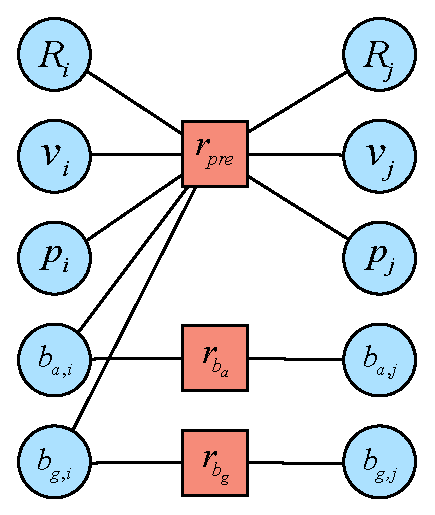
\includegraphics[width=0.4\textwidth]{resources/preintegration/preintegration-residual-graph.pdf}
	\caption{Graph optimization form of the preintegration factor}
	\label{fig:preintegration-residual-graph}
\end{figure}

Apart from placing all state variables in the same vertex, we can also choose a "disassembled form," where rotation, translation, linear velocity, and the two biases are each constructed as separate vertices, and then the Jacobians between these vertices are computed. If this approach is adopted, the number of Jacobian matrices will increase, but the dimensionality of individual Jacobians can be reduced (single Jacobians are typically $3 \times 3$, while the Jacobian of preintegration observations with respect to state variables becomes $9 \times 15$, with many zero blocks). Moreover, if we need to implement a tightly coupled visual or LiDAR system, since visual and LiDAR observation constraints are usually only related to $\mathbf{R}, \mathbf{t}$, some zero blocks in the Jacobian matrices can be avoided. In summary, both approaches have their merits. The code implementation in this book adopts the disassembled approach, where each state variable is written as a separate vertex to constrain them individually.

\subsection{Jacobians of Preintegration}  
\label{sec:preinteg-jacobians}  
Finally, we discuss the Jacobian matrices of preintegration with respect to the state variables. Since the preintegration measurements already summarize the IMU readings over a short period, the derivation of the residuals' Jacobians relative to the state variables becomes straightforward. Below, we derive them.  

First, consider rotation. Rotation depends on $\mathbf{R}_{i}$, $\mathbf{R}_j$, and $\mathbf{b}_{g,i}$. We derive it using the right perturbation on $\mathrm{SO}(3)$:  
\begin{equation}\label{key}  
	\begin{aligned}  
		\mathbf{r}_{\Delta \mathbf{R}_{ij}}\left(\mathbf{R}_i \mathrm{Exp} (\boldsymbol{\phi}_i)\right) &=   
		\mathrm{Log} \left( \Delta \tilde{\mathbf{R}}_{ij}^\top ((\mathbf{R}_i   
		\mathrm{Exp}(\boldsymbol{\phi_i}))^\top \mathbf{R}_j \right), \\  
		&= \mathrm{Log} \left( \Delta \tilde{\mathbf{R}}_{ij}^\top \mathrm{Exp} (-\boldsymbol{\phi}_i )   
		\mathbf{R}_i^\top \mathbf{R}_j \right), \\  
		&= \mathrm{Log} \left( \Delta \tilde{\mathbf{R}}_{ij}^\top \mathbf{R}_i^\top \mathbf{R}_j   
		\mathrm{Exp} (-\mathbf{R}_j^\top \mathbf{R}_i \boldsymbol{\phi}_i) \right), \\  
		&= \mathbf{r}_{\Delta \mathbf{R}_{ij}} - \mathbf{J}_r^{-1} (\mathbf{r}_{\Delta \mathbf{R}_{ij}}) \mathbf{R}_j^\top   
		\mathbf{R}_i \boldsymbol{\phi}_i.  
	\end{aligned}  
\end{equation}  

The derivative with respect to $\boldsymbol{\phi}_j$ is:  
\begin{equation}\label{key}  
	\begin{aligned}  
		\mathbf{r}_{\Delta \mathbf{R}_{ij}} (\mathbf{R}_j \mathrm{Exp}(\boldsymbol{\phi}_j)) &=   
		\mathrm{Log}\left(\Delta \tilde{\mathbf{R}}_{ij}^\top \mathbf{R}^\top_i \mathbf{R}_j   
		\mathrm{Exp} (\boldsymbol{\phi}_j ) \right), \\  
		&= \mathbf{r}_{\Delta \mathbf{R}_{ij}} + \mathbf{J}_r^{-1} (\mathbf{r}_{\Delta \mathbf{R}_{ij}}) \boldsymbol{\phi}_j.  
	\end{aligned}  
\end{equation}  

These derivations closely resemble those in pose graphs. However, dealing with the bias terms is slightly more involved. Note that during optimization, the bias terms are continuously updated, and each update uses \eqref{eq:update-bias} to correct the preintegration measurements. Since this process is iterative, we always have an initial measurement and a corrected measurement,  which must be taken into account during the derivation.

\subsection{Jacobians of Preintegration}
\label{sec:preinteg-jacobians}
Assume the initial bias for optimization is $\mathbf{b}_{g,i}$. At a certain iteration step, the current estimated bias correction is $\delta \mathbf{b}_{g,i}$, and the corrected preintegrated rotation measurement is $\Delta \tilde{\mathbf{R}}_{ij}^\prime = \Delta \tilde{\mathbf{R}}_{ij}(\mathbf{b}_{g,i} + \delta \mathbf{b}_{g,i})$, with the residual being $\mathbf{r}_{\Delta \mathbf{R}_{ij}}^\prime$. To compute the derivative, we further add $\tilde{\delta} \mathbf{b}_{g,i}$ to these two terms, yielding:

\begin{equation}\label{key}
	\small
	\begin{aligned}
		\mathbf{r}_{\Delta \mathbf{R}_{ij}} (\mathbf{b}_{g,i} + \delta \mathbf{b}_{g,i} + \tilde{\delta} \mathbf{b}_{g,i}) &= 
		\mathrm{Log}\left( \left( \Delta \tilde{\mathbf{R}}_{ij} \mathrm{Exp} \left( \frac{\partial \Delta 
			\tilde{\mathbf{R}}_{ij}}{\partial \mathbf{b}_{g,i}} (\delta \mathbf{b}_{g,i} + \tilde{\delta} \mathbf{b}_{g,i}) \right) 
		\right)^\top \mathbf{R}_i^\top \mathbf{R}_j \right), \\
		&\buildrel\text{BCH}\over\approx \mathrm{Log} \left( \left( \underbrace{\Delta \tilde{\mathbf{R}}_{ij} 
			\mathrm{Exp} (\frac{\partial \Delta \tilde{\mathbf{R}}_{ij}}{\partial \mathbf{b}_{g,i}} \delta 
			\mathbf{b}_{g,i})}_{\Delta \tilde{\mathbf{R}}_{ij}^\prime} \mathrm{Exp} (\mathbf{J}_{r, b} \frac{\partial \Delta 
			\tilde{\mathbf{R}}_{ij}}{\partial \mathbf{b}_{g,i}} \tilde{\delta} \mathbf{b}_{g,i}) \right)^\top 
		\mathbf{R}_i^\top \mathbf{R}_j \right), \\
		&= \mathrm{Log} \left( \mathrm{Exp} \left(-\mathbf{J}_{r,b} \frac{\partial \Delta 
			\tilde{\mathbf{R}}_{ij}}{\partial \mathbf{b}_{g,i}} \tilde{\delta} \mathbf{b}_{g,i} \right) \underbrace{(\Delta 
			\tilde{\mathbf{R}}_{ij}^\prime)^\top \mathbf{R}_i^\top \mathbf{R}_j}_{ \mathrm{Exp} \left( 
			\mathbf{r}_{ \Delta \mathbf{R}_{ij}}^\prime \right)} \right), \\
		&= \mathrm{Log} \left( \mathrm{Exp} \left(\mathbf{r}_{\Delta \mathbf{R}_{ij}}^\prime \right) \mathrm{Exp} 
		\left( - \mathrm{Exp}\left(\mathbf{r}_{\Delta \mathbf{R}_{ij}}^\prime \right)^\top \mathbf{J}_{r,b} 
		\frac{\partial \Delta \tilde{\mathbf{R}}_{ij}}{\partial \mathbf{b}_{g,i}} \tilde{\delta} \mathbf{b}_{g,i} \right)  \right), \\
		&\approx \mathbf{r}_{\Delta \mathbf{R}_{ij}}^\prime - \mathbf{J}_r^{-1} (\mathbf{r}_{\Delta \mathbf{R}_{ij}}^\prime ) 
		\mathrm{Exp}\left(\mathbf{r}_{\Delta \mathbf{R}_{ij}}^\prime \right)^\top \mathbf{J}_{r,b} \frac{\partial 
			\Delta \tilde{\mathbf{R}}_{ij}}{\partial \mathbf{b}_{g,i}} \tilde{\delta} \mathbf{b}_{g,i} .
	\end{aligned}
\end{equation}

Thus, we finally obtain:
\begin{equation}\label{key}
	\frac{\partial \mathbf{r}_{\Delta \mathbf{R}_{ij}}}{\partial \mathbf{b}_{g,i}} = - \mathbf{J}_r^{-1} (\mathbf{r}_{\Delta 
		\mathbf{R}_{ij}}^\prime ) \mathrm{Exp}\left(\mathbf{r}_{\Delta \mathbf{R}_{ij}}^\prime \right)^\top 
	\mathbf{J}_{r,b} \frac{\partial \Delta \tilde{\mathbf{R}}_{ij}}{\partial \mathbf{b}_{g,i}}.
\end{equation}

Next, consider the Jacobians for the velocity term. The velocity term is simpler, as it has a linear relationship with $\mathbf{v}_i$ and $\mathbf{v}_j$, yielding:
\begin{subequations}\label{key}
	\begin{align}
		\frac{ \partial \mathbf{r}_{\Delta \mathbf{v}_{ij}}}{\partial \mathbf{v}_i} &= -\mathbf{R}_i^\top, \\
		\frac{ \partial \mathbf{r}_{\Delta \mathbf{v}_{ij}}}{\partial \mathbf{v}_j} &= \mathbf{R}_i^\top.
	\end{align}
\end{subequations}

For the rotation part, a first-order Taylor expansion suffices:
\begin{equation}
	\begin{aligned}
		\mathbf{r}_{\Delta \mathbf{v}_{ij}} \left( \mathbf{R}_i \mathrm{Exp} (\delta \boldsymbol{\phi}_i)\right) &= 
		(\mathbf{R}_i \mathrm{Exp} (\delta \boldsymbol{\phi}_i)) ^\top (\mathbf{v}_j - \mathbf{v}_i - \mathbf{g} \Delta 
		t_{ij}) - \Delta \tilde{\mathbf{v}}_{ij}, \\
		&= (\mathbf{I} - \delta \boldsymbol{\phi}^\wedge_i) \mathbf{R}_i^\top  (\mathbf{v}_j - \mathbf{v}_i - \mathbf{g} 
		\Delta t_{ij}) - \Delta \tilde{\mathbf{v}}_{ij}, \\
		&= \mathbf{r}_{\Delta \mathbf{v}_{ij}} (\mathbf{R}_i) + \left(\mathbf{R}_i^\top  (\mathbf{v}_j - \mathbf{v}_i - \mathbf{g} 
		\Delta t_{ij}) \right)^\mathrm{\wedge} \delta \boldsymbol{\phi}_i.
	\end{aligned}
\end{equation}

The Jacobians of the velocity residual with respect to $\mathbf{b}_{g,i}$ and $\mathbf{b}_{a,i}$ depend only on $\Delta \tilde{\mathbf{v}}_{ij}$. Since the velocity residual term differs from it only by a negative sign, we simply need to add a negative sign to \eqref{eq:preinteg-jacob-bias}.

Finally, consider the translation part. The translation term depends linearly on $\mathbf{p}_i$, $\mathbf{p}_j$, $\mathbf{v}_i$, $\mathbf{R}_i$, and the two biases, making the Jacobians straightforward to derive:
\begin{subequations}\label{key}
	\begin{align}
		\frac{\partial \mathbf{r}_{\Delta \mathbf{p}_{ij}}}{\partial \mathbf{p}_i } &= -\mathbf{R}_i^\top, \\
		\frac{\partial \mathbf{r}_{\Delta \mathbf{p}_{ij}}}{\partial \mathbf{p}_j } &= \mathbf{R}_i^\top, \\
		\frac{\partial \mathbf{r}_{\Delta \mathbf{p}_{ij}}}{\partial \mathbf{v}_i } &= -\mathbf{R}_i^\top \Delta t_{ij}, \\
		\frac{\partial \mathbf{r}_{\Delta \mathbf{p}_{ij}}}{\partial \boldsymbol{\phi}_i } &= \left( 
		\mathbf{R}_i^\top \left(\mathbf{p}_j - \mathbf{p}_i - \mathbf{v}_i \Delta t_{ij} - \frac{1}{2}\mathbf{g} \Delta 
		t_{ij}^2 \right) \right)^\wedge.
	\end{align}
\end{subequations}
The residual for the biases simply requires adding a negative sign to Equation \eqref{eq:preinteg-jacob-bias}.

At this point, we have derived the derivative forms of the preintegrated measurements with respect to all state variables. If desired, we could write the preintegrated observations as a column vector, the state variables as another column vector, and combine all these Jacobian matrices accordingly. To save space, this book presents the preintegration matrices in their decomposed form.

\subsection{Summary}
Finally, we summarize the practical implementation process of the aforementioned preintegration in real-world applications.

In a system composed of keyframes, we can initiate the preintegration process starting from any keyframe at any given time and terminate it at any desired moment. Subsequently, we can extract the preintegrated measurements, noise terms, and various accumulated Jacobians to constrain the states between two keyframes. Based on previous discussions, once preintegration begins, whenever a new IMU measurement arrives, our program should perform the following tasks:
\begin{enumerate}
	\item 
	Compute the three \textbf{preintegrated measurements} using Equation \eqref{eq:def-preintegration} based on the previous data: $\Delta \tilde{\mathbf{R}}_{ij}, \Delta \tilde{\mathbf{v}}_{ij}, \Delta \tilde{\mathbf{p}}_{ij}$;
	\item Calculate the \textbf{covariance matrices} of the three noise terms, which will serve as the information matrices for subsequent graph optimization;
	\item Compute the \textbf{Jacobian matrices} of the preintegrated measurements with respect to the biases - five in total;
\end{enumerate}

Upon completion of the preintegration calculations, these results can be extracted and applied during the optimization process.

\section{Practice: Implementation of Preintegration}
\subsection{Implementing the Preintegration Class}

Following the derivations from the previous section, we now implement the preintegration program. The implementation mainly consists of two parts: the computation of preintegration itself, and its integration into graph optimization. The former is relatively simple as it only involves IMU measurements, while the latter depends on the specific graph optimization framework - in this book we'll implement it using the g2o framework.

First, let's implement the preintegration structure itself. A preintegration class should store the following data:
\begin{itemize}
	\item Preintegrated measurements $\Delta \tilde{\mathbf{R}}_{ij}, \Delta \tilde{\mathbf{p}}_{ij}, \Delta \tilde{\mathbf{v}}_{ij}$;
	\item IMU biases at the start of preintegration $\mathbf{b}_g, \mathbf{b}_a$;
	\item Measurement noise covariance $\boldsymbol{\Sigma}_{i,k+1}$ during integration, as specified by Equation \eqref{eq:preinteg-motion-noise};
	\item Jacobian matrices of integrated quantities with respect to IMU biases (see Equation \eqref{eq:preinteg-jacob-bias-inc});
	\item Total integration time $\Delta t_{ij}$.
\end{itemize}

The above are all essential information. Additionally, we may choose to store IMU measurements in the preintegration class (though this is optional since they're already integrated). The IMU measurement noise and bias random walk noise can also be included as configuration parameters. Here's the basic implementation of such a preintegration class:

\begin{lstlisting}[language=c++, caption=src/ch4/imu\_preintegration.h]
class IMUPreintegration {
	public:
	/// Other functions omitted
	struct Options {
		Options() {}
		Vec3d init_bg_ = Vec3d::Zero();  // Initial bias
		Vec3d init_ba_ = Vec3d::Zero();  // Initial bias
		double noise_gyro_ = 1e-2;       // Gyro noise (std dev)
		double noise_acce_ = 1e-1;       // Accelerometer noise (std dev)
	};
	
	public:
	double dt_ = 0;                          // Total preintegration time
	Mat9d cov_ = Mat9d::Zero();              // Accumulated noise matrix
	Mat6d noise_gyro_acce_ = Mat6d::Zero();  // Measurement noise matrix
	
	// Biases
	Vec3d bg_ = Vec3d::Zero();
	Vec3d ba_ = Vec3d::Zero();
	
	// Preintegrated measurements
	SO3 dR_;
	Vec3d dv_ = Vec3d::Zero();
	Vec3d dp_ = Vec3d::Zero();
	
	// Jacobian matrices
	Mat3d dR_dbg_ = Mat3d::Zero();
	Mat3d dV_dbg_ = Mat3d::Zero();
	Mat3d dV_dba_ = Mat3d::Zero();
	Mat3d dP_dbg_ = Mat3d::Zero();
	Mat3d dP_dba_ = Mat3d::Zero();
};
\end{lstlisting}

The variables maintained by this class correspond to those introduced earlier. Note that the IMU bias-related noise terms are not directly part of the preintegration class - we'll move them to the optimization class. This class mainly handles the preintegration of IMU data and provides the integrated measurements and noise values.

\section{Practice: Implementation of Preintegration}
\subsection{Implementing the Single IMU Integration}

The implementation of single IMU integration is as follows:
\begin{lstlisting}[language=c++,caption=src/ch4/imu\_preintegration.cc]
void IMUPreintegration::Integrate(const IMU &imu, double dt) {
	// Remove bias from measurements
	Vec3d gyr = imu.gyro_ - bg_;  // Gyroscope
	Vec3d acc = imu.acce_ - ba_;  // Accelerometer
	
	// Update dv, dp, see (4.7)
	dp_ = dp_ + dv_ * dt + 0.5f * dR_.matrix() * acc * dt * dt;
	dv_ = dv_ + dR_ * acc * dt;
	
	// dR update deferred as current dR needed for A, B matrices
	
	// Jacobian coefficients for motion equation, matrices A,B, see (4.29)
	// Other terms handled later
	Eigen::Matrix<double, 9, 9> A;
	A.setIdentity();
	Eigen::Matrix<double, 9, 6> B;
	B.setZero();
	
	Mat3d acc_hat = SO3::hat(acc);
	double dt2 = dt * dt;
	
	// NOTE: Top-left blocks of A, B differ slightly from formula
	A.block<3, 3>(3, 0) = -dR_.matrix() * dt * acc_hat;
	A.block<3, 3>(6, 0) = -0.5f * dR_.matrix() * acc_hat * dt2;
	A.block<3, 3>(6, 3) = dt * Mat3d::Identity();
	
	B.block<3, 3>(3, 3) = dR_.matrix() * dt;
	B.block<3, 3>(6, 3) = 0.5f * dR_.matrix() * dt2;
	
	// Update Jacobians, see (4.39)
	dP_dba_ = dP_dba_ + dV_dba_ * dt - 0.5f * dR_.matrix() * dt2;                      // (4.39d)
	dP_dbg_ = dP_dbg_ + dV_dbg_ * dt - 0.5f * dR_.matrix() * dt2 * acc_hat * dR_dbg_;  // (4.39e)
	dV_dba_ = dV_dba_ - dR_.matrix() * dt;                                             // (4.39b)
	dV_dbg_ = dV_dbg_ - dR_.matrix() * dt * acc_hat * dR_dbg_;                         // (4.39c)
	
	// Rotation part
	Vec3d omega = gyr * dt;         // Rotation amount
	Mat3d rightJ = SO3::jr(omega);  // Right Jacobian
	SO3 deltaR = SO3::exp(omega);   // After exp
	dR_ = dR_ * deltaR;             // (4.7a)
	
	A.block<3, 3>(0, 0) = deltaR.matrix().transpose();
	B.block<3, 3>(0, 0) = rightJ * dt;
	
	// Update noise term
	cov_ = A * cov_ * A.transpose() + B * noise_gyro_acce_ * B.transpose();
	
	// Update dR_dbg
	dR_dbg_ = deltaR.matrix().transpose() * dR_dbg_ - rightJ * dt;  // (4.39a)
	
	// Increment integration time
	dt_ += dt;
}
\end{lstlisting}

We've added equation numbers in the code comments to help readers locate corresponding formulas. Overall, it updates internal member variables in the following order:
\begin{enumerate}
	\item Updates position and velocity measurements;
	\item Updates noise matrix for motion model;
	\item Updates Jacobians of measurements with respect to biases;
	\item Updates rotation measurements;
	\item Updates integration time.
\end{enumerate}

This completes one IMU data operation. Note that without optimization, preintegration and direct integration produce identical results - both integrate IMU data. After preintegration, we can predict from initial to final state similar to ESKF. The prediction function is straightforward:

\begin{lstlisting}[language=c++,caption=src/ch4/imu\_preintegraion.cc]
NavStated IMUPreintegration::Predict(const sad::NavStated &start, const Vec3d &grav) {
	SO3 Rj = start.R_ * dR_;
	Vec3d vj = start.R_ * dv_ + start.v_ + grav * dt_;
	Vec3d pj = start.R_ * dp_ + start.p_ + start.v_ * dt_ + 0.5f * grav * dt_ * dt_;
	
	auto state = NavStated(start.timestamp_ + dt_, Rj, pj, vj);
	state.bg_ = bg_;
	state.ba_ = ba_;
	return state;
}
\end{lstlisting}

Unlike ESKF, preintegration can predict multiple IMU measurements and predict forward from any starting time, while ESKF typically only predicts from current state to next timestamp for single IMU measurement.

Next, we write a test program to verify whether there is a significant difference between preintegration and direct integration when a constant angular velocity and acceleration are present in a single direction. This method is very effective for identifying obvious errors in the code. Since we implemented the ESKF in the previous chapter, we can also compare the prediction process of ESKF with preintegration. If the initial states are the same, the results should be completely consistent.

\begin{lstlisting}[language=c++,caption=src/ch4/test\_preintegraion.cc]
TEST(PREINTEGRATION_TEST, ROTATION_TEST) {
	// Test the case of preintegration under constant angular velocity
	double imu_time_span = 0.01;       // IMU measurement interval
	Vec3d constant_omega(0, 0, M_PI);  // Angular velocity of 180 deg/s, rotating for 1 second equals 180 degrees
	Vec3d gravity(0, 0, -9.8);         // Z is upward, gravity is in the negative direction
	
	sad::NavStated start_status(0), end_status(1.0);
	sad::IMUPreintegration pre_integ;
	
	// Compare with direct integration
	Sophus::SO3d R;
	Vec3d t = Vec3d::Zero();
	Vec3d v = Vec3d::Zero();
	
	for (int i = 1; i <= 100; ++i) {
		double time = imu_time_span * i;
		Vec3d acce = -gravity;  // Accelerometer should measure an upward force
		pre_integ.Integrate(sad::IMU(time, constant_omega, acce), imu_time_span);
		
		sad::NavStated this_status = pre_integ.Predict(start_status, gravity);
		
		t = t + v * imu_time_span + 0.5 * gravity * imu_time_span * imu_time_span +
		0.5 * (R * acce) * imu_time_span * imu_time_span;
		v = v + gravity * imu_time_span + (R * acce) * imu_time_span;
		R = R * Sophus::SO3d::exp(constant_omega * imu_time_span);
		
		// Verify that under simple conditions, direct integration and preintegration yield the same result
		EXPECT_NEAR(t[0], this_status.p_[0], 1e-2);
		EXPECT_NEAR(t[1], this_status.p_[1], 1e-2);
		EXPECT_NEAR(t[2], this_status.p_[2], 1e-2);
		
		EXPECT_NEAR(v[0], this_status.v_[0], 1e-2);
		EXPECT_NEAR(v[1], this_status.v_[1], 1e-2);
		EXPECT_NEAR(v[2], this_status.v_[2], 1e-2);
		
		EXPECT_NEAR(R.unit_quaternion().x(), this_status.R_.unit_quaternion().x(), 1e-4);
		EXPECT_NEAR(R.unit_quaternion().y(), this_status.R_.unit_quaternion().y(), 1e-4);
		EXPECT_NEAR(R.unit_quaternion().z(), this_status.R_.unit_quaternion().z(), 1e-4);
		EXPECT_NEAR(R.unit_quaternion().w(), this_status.R_.unit_quaternion().w(), 1e-4);
	}
	
	end_status = pre_integ.Predict(start_status);
	
	LOG(INFO) << "preinteg result: ";
	LOG(INFO) << "end rotation: \n" << end_status.R_.matrix();
	LOG(INFO) << "end trans: \n" << end_status.p_.transpose();
	LOG(INFO) << "end v: \n" << end_status.v_.transpose();
	
	LOG(INFO) << "direct integ result: ";
	LOG(INFO) << "end rotation: \n" << R.matrix();
	LOG(INFO) << "end trans: \n" << t.transpose();
	LOG(INFO) << "end v: \n" << v.transpose();
	SUCCEED();
}
\end{lstlisting}

This code uses the gtest framework to verify whether there is a significant difference between IMU integration and preintegration under a fixed angular velocity measurement along the $Z$ axis. The same file also contains tests for constant acceleration and comparisons with ESKF. Since the code is very similar, we do not list it here. Readers can run this code to check whether the IMU operations in the preintegration module are implemented correctly.

\subsection{Graph Optimization Vertices for Pre-integration}

Next, we will implement the graph optimization related to pre-integration. Compared to the filter framework, the graph optimization framework is slightly more complex but offers greater flexibility in usage. We will introduce the variables and classes related to graph optimization one by one.

First, our 15-dimensional or 18-dimensional state variables should correspond to the vertices in graph optimization. They use generalized addition to implement operations on matrix manifolds and tangent spaces. This book adopts a \textbf{bulk} form, so each state is divided into four types of vertices: pose, velocity, gyroscope bias, and accelerometer bias. The latter three are essentially variables in $\mathbb{R}^3$ and can be directly implemented using inheritance.

\begin{lstlisting}[language=c++,caption=src/common/g2o\_types.h]
class VertexPose : public g2o::BaseVertex<6, SE3> {
	public:
	EIGEN_MAKE_ALIGNED_OPERATOR_NEW
	VertexPose() {}
	
	virtual void oplusImpl(const double* update_) {
		_estimate.so3() = _estimate.so3() * SO3::exp(Eigen::Map<const Vec3d>(&update_[0]));  // Rotation part
		_estimate.translation() += Eigen::Map<const Vec3d>(&update_[3]);                     // Translation part
		updateCache();
	}
};

/**
* Velocity vertex, simply Vec3d
*/
class VertexVelocity : public g2o::BaseVertex<3, Vec3d> {
	public:
	VertexVelocity() {}
	virtual void oplusImpl(const double* update_) {
		Vec3d uv;
		uv << update_[0], update_[1], update_[2];
		setEstimate(estimate() + uv);
	}
};

/**
* Gyroscope bias vertex, also Vec3d, inherits from velocity vertex
*/
class VertexGyroBias : public VertexVelocity {
	public:
	VertexGyroBias() {}
};

/**
* Accelerometer bias vertex, Vec3d, also inherits from velocity vertex
*/
class VertexAccBias : public VertexVelocity {
	public:
	VertexAccBias() {}
};
\end{lstlisting}

We have only listed the key implementation parts, omitting some default constructors. We combine rotation and translation in the same VertexPose vertex. Special attention should be paid to the variable ordering here. Inside VertexPose, rotation comes first followed by translation, so the Jacobian matrix ordering must correspond accordingly.

\subsection{Graph Optimization Edges for Pre-integration Scheme}

Next, we will formulate the prediction and update equations from the previous chapter's GINS system into graph optimization form. Let's summarize the optimization-related edges as follows:
\begin{enumerate}
	\item Pre-integration edges, which constrain the 15-dimensional state from the previous timestamp to the rotation, translation, and velocity at the next timestamp;
	\item Bias random walk edges (two types), connecting bias states between two timestamps;
	\item GNSS observation edges. Since we use 6-DOF observations, they associate with the pose at a single timestamp;
	\item Prior information, characterizing the state distribution at the previous timestamp and associating with the 15-dimensional state at that time;
	\item Wheel odometer observation edges, associating with the velocity vertex at the previous timestamp.
\end{enumerate}

We will implement these components sequentially. First is the most complex pre-integration edge. Its error function and Jacobian function are as follows:
\begin{lstlisting}[language=c++,caption=src/ch4/g2o\_types.cc]
class EdgeInertial : public g2o::BaseMultiEdge<9, Vec9d> {
	public:
	EIGEN_MAKE_ALIGNED_OPERATOR_NEW
	
	/**
	* The constructor needs to specify the pre-integration class object
	* @param preinteg   Pointer to the pre-integration object
	* @param gravity    Gravity vector
	* @param weight     Weight
	*/
	EdgeInertial(std::shared_ptr<IMUPreintegration> preinteg, const Vec3d& gravity, double weight = 1.0);
	
	void computeError() override;
	void linearizeOplus() override;
	private:
	const double dt_;
	std::shared_ptr<IMUPreintegration> preint_ = nullptr;
	Vec3d grav_;
};

EdgeInertial::EdgeInertial(std::shared_ptr<IMUPreintegration> preinteg, const Vec3d& gravity, double weight)
: preint_(preinteg), dt_(preinteg->dt_) {
	resize(6);  // 6 connected vertices
	grav_ = gravity;
	setInformation(preinteg->cov_.inverse() * weight);
}

void EdgeInertial::computeError() {
	auto* p1 = dynamic_cast<const VertexPose*>(_vertices[0]);
	auto* v1 = dynamic_cast<const VertexVelocity*>(_vertices[1]);
	auto* bg1 = dynamic_cast<const VertexGyroBias*>(_vertices[2]);
	auto* ba1 = dynamic_cast<const VertexAccBias*>(_vertices[3]);
	auto* p2 = dynamic_cast<const VertexPose*>(_vertices[4]);
	auto* v2 = dynamic_cast<const VertexVelocity*>(_vertices[5]);
	
	Vec3d bg = bg1->estimate();
	Vec3d ba = ba1->estimate();
	
	const SO3 dR = preint_->GetDeltaRotation(bg);
	const Vec3d dv = preint_->GetDeltaVelocity(bg, ba);
	const Vec3d dp = preint_->GetDeltaPosition(bg, ba);
	
	/// Pre-integration error terms (4.41)
	const Vec3d er = (dR.inverse() * p1->estimate().so3().inverse() * p2->estimate().so3()).log();
	Mat3d RiT = p1->estimate().so3().inverse().matrix();
	const Vec3d ev = RiT * (v2->estimate() - v1->estimate() - grav_ * dt_) - dv;
	const Vec3d ep = RiT * (p2->estimate().translation() - p1->estimate().translation() - v1->estimate() * dt_ -
	grav_ * dt_ * dt_ / 2) -
	dp;
	_error << er, ev, ep;
}

void EdgeInertial::linearizeOplus() {
	auto* p1 = dynamic_cast<const VertexPose*>(_vertices[0]);
	auto* v1 = dynamic_cast<const VertexVelocity*>(_vertices[1]);
	auto* bg1 = dynamic_cast<const VertexGyroBias*>(_vertices[2]);
	auto* ba1 = dynamic_cast<const VertexAccBias*>(_vertices[3]);
	auto* p2 = dynamic_cast<const VertexPose*>(_vertices[4]);
	auto* v2 = dynamic_cast<const VertexVelocity*>(_vertices[5]);
	
	Vec3d bg = bg1->estimate();
	Vec3d ba = ba1->estimate();
	Vec3d dbg = bg - preint_->bg_;
	
	// Intermediate symbols
	const SO3 R1 = p1->estimate().so3();
	const SO3 R1T = R1.inverse();
	const SO3 R2 = p2->estimate().so3();
	
	auto dR_dbg = preint_->dR_dbg_;
	auto dv_dbg = preint_->dV_dbg_;
	auto dp_dbg = preint_->dP_dbg_;
	auto dv_dba = preint_->dV_dba_;
	auto dp_dba = preint_->dP_dba_;
	
	// Estimates
	Vec3d vi = v1->estimate();
	Vec3d vj = v2->estimate();
	Vec3d pi = p1->estimate().translation();
	Vec3d pj = p2->estimate().translation();
	
	const SO3 dR = preint_->GetDeltaRotation(bg);
	const SO3 eR = SO3(dR).inverse() * R1T * R2;
	const Vec3d er = eR.log();
	const Mat3d invJr = SO3::jr_inv(eR);
	
	/// Jacobian matrices
	/// Note there are 3 indices: vertex index, own error row, and vertex internal variable column
	/// Variable order: pose1(R1,p1), v1, bg1, ba1, pose2(R2,p2), v2
	/// Residual order: eR, ev, ep, with residual order as rows and variable order as columns
	
	//       | R1 | p1 | v1 | bg1 | ba1 | R2 | p2 | v2 |
	//  vert | 0       | 1  | 2   | 3   | 4       | 5  |
	//  col  | 0    3  | 0  | 0   | 0   | 0    3  | 0  |
	//    row
	//  eR 0 |
	//  ev 3 |
	//  ep 6 |
	
	/// Residual w.r.t R1, 9x3
	_jacobianOplus[0].setZero();
	// dR/dR1, 4.42
	_jacobianOplus[0].block<3, 3>(0, 0) = -invJr * (R2.inverse() * R1).matrix();
	// dv/dR1, 4.47
	_jacobianOplus[0].block<3, 3>(3, 0) = SO3::hat(R1T * (vj - vi - grav_ * dt_));
	// dp/dR1, 4.48d
	_jacobianOplus[0].block<3, 3>(6, 0) = SO3::hat(R1T * (pj - pi - v1->estimate() * dt_ - 0.5 * grav_ * dt_ * dt_));
	
	/// Residual w.r.t p1, 9x3
	// dp/dp1, 4.48a
	_jacobianOplus[0].block<3, 3>(6, 3) = -R1T.matrix();
	
	/// Residual w.r.t v1, 9x3
	_jacobianOplus[1].setZero();
	// dv/dv1, 4.46a
	_jacobianOplus[1].block<3, 3>(3, 0) = -R1T.matrix();
	// dp/dv1, 4.48c
	_jacobianOplus[1].block<3, 3>(6, 0) = -R1T.matrix() * dt_;
	
	/// Residual w.r.t bg1
	_jacobianOplus[2].setZero();
	// dR/dbg1, 4.45
	_jacobianOplus[2].block<3, 3>(0, 0) = -invJr * eR.inverse().matrix() * SO3::jr((dR_dbg * dbg).eval()) * dR_dbg;
	// dv/dbg1
	_jacobianOplus[2].block<3, 3>(3, 0) = -dv_dbg;
	// dp/dbg1
	_jacobianOplus[2].block<3, 3>(6, 0) = -dp_dbg;
	
	/// Residual w.r.t ba1
	_jacobianOplus[3].setZero();
	// dv/dba1
	_jacobianOplus[3].block<3, 3>(3, 0) = -dv_dba;
	// dp/dba1
	_jacobianOplus[3].block<3, 3>(6, 0) = -dp_dba;
	
	/// Residual w.r.t pose2
	_jacobianOplus[4].setZero();
	// dr/dr2, 4.43
	_jacobianOplus[4].block<3, 3>(0, 0) = invJr;
	// dp/dp2, 4.48b
	_jacobianOplus[4].block<3, 3>(6, 3) = R1T.matrix();
	
	/// Residual w.r.t v2
	_jacobianOplus[5].setZero();
	// dv/dv2, 4,46b
	_jacobianOplus[5].block<3, 3>(3, 0) = R1T.matrix();  // OK
}
\end{lstlisting}

We have also provided corresponding formulas in the comments for readers to compare. During implementation, we must be careful with the order of Jacobian matrices here. They actually have three indices: \textbf{which vertex}, the \textbf{row of the error term}, and the \textbf{column of the vertex's internal variables}. For example, if we want to compute the Jacobian block of the pre-integration $\Delta \tilde{\mathbf{p}}_{ij}$ with respect to the translation part of the second pose, i.e., $\mathbf{p}_j$, then the corresponding Jacobian block should be located at the 4th vertex, 6th row, and 3rd column. Here, the 4th vertex means the pose vertex at time $j$ is the 4th vertex of the pre-integration edge, the 6th row means $\delta \tilde{\mathbf{p}}_{ij}$ is the 6th row in the pre-integration observation, and the 3rd column means $\mathbf{p}_j$ is the 3rd column in VertexPose. Regardless of which optimization framework we use, when defining Jacobian matrices ourselves, we will encounter such matrix block ordering issues when dealing with connections between multiple vertices. This is an error-prone area.

Now let's define the edges for biases, GNSS, prior states, and odometry. The two bias edges are essentially identical, so we'll only show one:

\begin{lstlisting}[language=c++,caption=src/common/g2o\_types.h]
class EdgeGyroRW : public g2o::BaseBinaryEdge<3, Vec3d, VertexGyroBias, VertexGyroBias> {
	public:	
	void computeError() {
		const VertexGyroBias* VG1 = static_cast<const VertexGyroBias*>(_vertices[0]);
		const VertexGyroBias* VG2 = static_cast<const VertexGyroBias*>(_vertices[1]);
		_error = VG2->estimate() - VG1->estimate();
	}
	
	virtual void linearizeOplus() {
		_jacobianOplusXi = -Mat3d::Identity();
		_jacobianOplusXj.setIdentity();
	}
};

/**
* Prior for previous frame's IMU pvq bias
* info is specified externally, given by marginalization in time window
*
* Vertex order: pose, v, bg, ba
* Residual order: R, p, v, bg, ba, 15-dimensional
*/
class EdgePriorPoseNavState : public g2o::BaseMultiEdge<15, Vec15d> {
	public:
	void computeError();
	virtual void linearizeOplus();
	NavStated state_;
};

void EdgePriorPoseNavState::computeError() {
	auto* vp = dynamic_cast<const VertexPose*>(_vertices[0]);
	auto* vv = dynamic_cast<const VertexVelocity*>(_vertices[1]);
	auto* vg = dynamic_cast<const VertexGyroBias*>(_vertices[2]);
	auto* va = dynamic_cast<const VertexAccBias*>(_vertices[3]);
	
	const Vec3d er = SO3(state_.R_.matrix().transpose() * vp->estimate().so3().matrix()).log();
	const Vec3d ep = vp->estimate().translation() - state_.p_;
	const Vec3d ev = vv->estimate() - state_.v_;
	const Vec3d ebg = vg->estimate() - state_.bg_;
	const Vec3d eba = va->estimate() - state_.ba_;
	
	_error << er, ep, ev, ebg, eba;
}

void EdgePriorPoseNavState::linearizeOplus() {
	const auto* vp = dynamic_cast<const VertexPose*>(_vertices[0]);
	const Vec3d er = SO3(state_.R_.matrix().transpose() * vp->estimate().so3().matrix()).log();
	
	/// Note there are 3 indices: vertex index, error row, and vertex internal variable column
	_jacobianOplus[0].setZero();
	_jacobianOplus[0].block<3, 3>(0, 0) = SO3::jr_inv(er);    // dr/dr
	_jacobianOplus[0].block<3, 3>(3, 3) = Mat3d::Identity();  // dp/dp
	_jacobianOplus[1].setZero();
	_jacobianOplus[1].block<3, 3>(6, 0) = Mat3d::Identity();  // dv/dv
	_jacobianOplus[2].setZero();
	_jacobianOplus[2].block<3, 3>(9, 0) = Mat3d::Identity();  // dbg/dbg
	_jacobianOplus[3].setZero();
	_jacobianOplus[3].block<3, 3>(12, 0) = Mat3d::Identity();  // dba/dba
}

class EdgeGNSS : public g2o::BaseUnaryEdge<6, SE3, VertexPose> {
	public:
	void computeError() override {
		VertexPose* v = (VertexPose*)_vertices[0];
		_error.head<3>() = (_measurement.so3().inverse() * v->estimate().so3()).log();
		_error.tail<3>() = v->estimate().translation() - _measurement.translation();
	};
	
	void linearizeOplus() override {
		VertexPose* v = (VertexPose*)_vertices[0];
		// jacobian 6x6
		_jacobianOplusXi.setZero();
		_jacobianOplusXi.block<3, 3>(0, 0) = (_measurement.so3().inverse() * v->estimate().so3()).jr_inv();  // dR/dR
		_jacobianOplusXi.block<3, 3>(3, 3) = Mat3d::Identity();                        
	}
};
\end{lstlisting}

Most of the Jacobian matrices here are quite straightforward, and readers should be able to derive them themselves.

\subsection{Implementation of GINS Based on Pre-integration and Graph Optimization}

Finally, we utilize the graph optimization edges defined earlier to implement a GNSS/INS fusion positioning system similar to the ESKF. Readers can also use this experiment to gain deeper insights into the similarities and differences between graph optimization and filter-based approaches. This graph optimization-based GINS system follows essentially the same logic as the ESKF, still requiring static IMU initialization to determine the initial IMU biases and gravity direction. We encapsulate these logical processes in a separate class while focusing on how this graph optimization model is constructed. The basic workflow is as follows:

\begin{enumerate}
	\item 
	We obtain initial biases and gravity direction through an external static IMU initialization algorithm, then use the first GNSS measurement with attitude information to determine the initial position and orientation. When both IMU and GNSS data become available, we begin prediction and optimization.
	
	\item When IMU data arrives, we use the pre-integrator to accumulate IMU integration information.
	
	\item When odometry data arrives, we record it as the most recent velocity observation and retain its readings.
	
	\item When GNSS data arrives, we construct a graph optimization problem between \textbf{the previous timestamp's} GNSS and \textbf{the current timestamp's} GNSS. The nodes and edges of this problem are defined as:
	\begin{itemize}
		\item Nodes: Pose, velocity, and both bias terms (gyro and accelerometer) from the previous and current timestamps - totaling 8 vertices.
		\item Edges: Pre-integration observation edge between two timestamps, GNSS observation edges for both timestamps, prior edge for the previous timestamp, two bias random walk edges, and velocity observation edge - making 7 edges in total.
	\end{itemize}
	
	\item We use the predicted values from IMU pre-integration as initial values for optimization. Alternatively, GNSS observations could also be used for initialization. While these two initialization methods yield different starting points, they produce similar results in our current implementation. Readers are encouraged to experiment with both approaches.
\end{enumerate}

\begin{figure}[!htp]
	\centering
	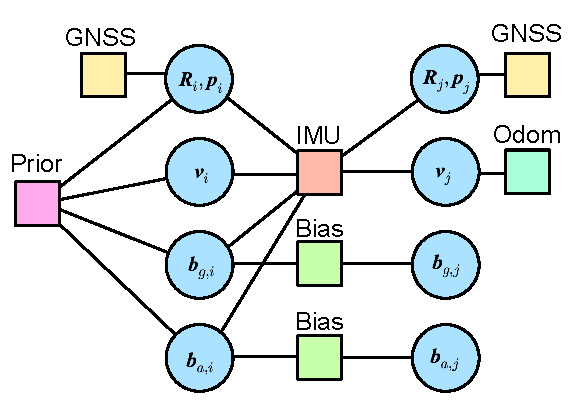
\includegraphics[width=0.5\textwidth]{preintegration/real-factor-graph}
	\caption{Actual graph optimization structure used in the GINS case study}
	\label{fig:real-factor-graph}
\end{figure}

The complete graph optimization structure is shown in Figure~\ref{fig:real-factor-graph}~. We implement GINS as a class that handles IMU, Odom and GNSS observations:

\begin{lstlisting}[language=c++,caption=src/ch4/gins\_pre\_integ.cc]
	void GinsPreInteg::AddImu(const IMU& imu) {
		if (first_gnss_received_ && first_imu_received_) {
			pre_integ_->Integrate(imu, imu.timestamp_ - last_imu_.timestamp_);
		}
		
		first_imu_received_ = true;
		last_imu_ = imu;
		current_time_ = imu.timestamp_;
	}
	
	void GinsPreInteg::AddOdom(const sad::Odom& odom) {
		last_odom_ = odom;
		last_odom_set_ = true;
	}
	
	void GinsPreInteg::AddGnss(const GNSS& gnss) {
		this_frame_ = std::make_shared<NavStated>(current_time_);
		this_gnss_ = gnss;
		
		if (!first_gnss_received_) {
			if (!gnss.heading_valid_) {
				// First GNSS must have valid heading
				return;
			}
			
			// First GNSS measurement sets initial pose
			this_frame_->timestamp_ = gnss.unix_time_;
			this_frame_->p_ = gnss.utm_pose_.translation();
			this_frame_->R_ = gnss.utm_pose_.so3();
			this_frame_->v_.setZero();
			this_frame_->bg_ = options_.preinteg_options_.init_bg_;
			this_frame_->ba_ = options_.preinteg_options_.init_ba_;
			
			pre_integ_ = std::make_shared<IMUPreintegration>(options_.preinteg_options_);
			
			last_frame_ = this_frame_;
			last_gnss_ = this_gnss_;
			first_gnss_received_ = true;
			current_time_ = gnss.unix_time_;
			return;
		}
		
		current_time_ = gnss.unix_time_;
		*this_frame_ = pre_integ_->Predict(*last_frame_, options_.gravity_);
		
		Optimize();
		
		last_frame_ = this_frame_;
		last_gnss_ = this_gnss_;
	}
\end{lstlisting}

The processing functions mainly handle workflow logic, with the key content being the Optimize function:

\begin{lstlisting}[language=c++,caption=src/ch4/gins\_pre\_integ.cc]
	void GinsPreInteg::Optimize() {
		if (pre_integ_->dt_ < 1e-3) {
			// No integration available
			return;
		}
		
		LOG(INFO) << "calling optimization";
		
		using BlockSolverType = g2o::BlockSolverX;
		using LinearSolverType = g2o::LinearSolverEigen<BlockSolverType::PoseMatrixType>;
		
		auto* solver = new g2o::OptimizationAlgorithmLevenberg(
		g2o::make_unique<BlockSolverType>(g2o::make_unique<LinearSolverType>()));
		g2o::SparseOptimizer optimizer;
		optimizer.setAlgorithm(solver);
		
		// Previous timestamp vertices: pose, v, bg, ba
		auto v0_pose = new VertexPose();
		v0_pose->setId(0);
		v0_pose->setEstimate(last_frame_->GetSE3());
		optimizer.addVertex(v0_pose);
		
		auto v0_vel = new VertexVelocity();
		v0_vel->setId(1);
		v0_vel->setEstimate(last_frame_->v_);
		optimizer.addVertex(v0_vel);
		
		auto v0_bg = new VertexGyroBias();
		v0_bg->setId(2);
		v0_bg->setEstimate(last_frame_->bg_);
		optimizer.addVertex(v0_bg);
		
		auto v0_ba = new VertexAccBias();
		v0_ba->setId(3);
		v0_ba->setEstimate(last_frame_->ba_);
		optimizer.addVertex(v0_ba);
		
		// Current timestamp vertices: pose, v, bg, ba
		auto v1_pose = new VertexPose();
		v1_pose->setId(4);
		v1_pose->setEstimate(this_frame_->GetSE3());
		optimizer.addVertex(v1_pose);
		
		auto v1_vel = new VertexVelocity();
		v1_vel->setId(5);
		v1_vel->setEstimate(this_frame_->v_);
		optimizer.addVertex(v1_vel);
		
		auto v1_bg = new VertexGyroBias();
		v1_bg->setId(6);
		v1_bg->setEstimate(this_frame_->bg_);
		optimizer.addVertex(v1_bg);
		
		auto v1_ba = new VertexAccBias();
		v1_ba->setId(7);
		v1_ba->setEstimate(this_frame_->ba_);
		optimizer.addVertex(v1_ba);
		
		// Pre-integration edge
		auto edge_inertial = new EdgeInertial(pre_integ_, options_.gravity_);
		edge_inertial->setVertex(0, v0_pose);
		edge_inertial->setVertex(1, v0_vel);
		edge_inertial->setVertex(2, v0_bg);
		edge_inertial->setVertex(3, v0_ba);
		edge_inertial->setVertex(4, v1_pose);
		edge_inertial->setVertex(5, v1_vel);
		auto* rk = new g2o::RobustKernelHuber();
		rk->setDelta(200.0);
		edge_inertial->setRobustKernel(rk);
		optimizer.addEdge(edge_inertial);
		
		// Bias random walk edges
		auto* edge_gyro_rw = new EdgeGyroRW();
		edge_gyro_rw->setVertex(0, v0_bg);
		edge_gyro_rw->setVertex(1, v1_bg);
		edge_gyro_rw->setInformation(options_.bg_rw_info_);
		optimizer.addEdge(edge_gyro_rw);
		
		auto* edge_acc_rw = new EdgeAccRW();
		edge_acc_rw->setVertex(0, v0_ba);
		edge_acc_rw->setVertex(1, v1_ba);
		edge_acc_rw->setInformation(options_.ba_rw_info_);
		optimizer.addEdge(edge_acc_rw);
		
		// Previous timestamp prior
		auto* edge_prior = new EdgePriorPoseNavState(*last_frame_, prior_info_);
		edge_prior->setVertex(0, v0_pose);
		edge_prior->setVertex(1, v0_vel);
		edge_prior->setVertex(2, v0_bg);
		edge_prior->setVertex(3, v0_ba);
		optimizer.addEdge(edge_prior);
		
		// GNSS edges
		auto edge_gnss0 = new EdgeGNSS(v0_pose, last_gnss_.utm_pose_);
		edge_gnss0->setInformation(options_.gnss_info_);
		optimizer.addEdge(edge_gnss0);
		
		auto edge_gnss1 = new EdgeGNSS(v1_pose, this_gnss_.utm_pose_);
		edge_gnss1->setInformation(options_.gnss_info_);
		optimizer.addEdge(edge_gnss1);
		
		// Odom edge
		EdgeEncoder3D* edge_odom = nullptr;
		Vec3d vel_world = Vec3d::Zero();
		Vec3d vel_odom = Vec3d::Zero();
		if (last_odom_set_) {
			// velocity obs
			double velo_l =
			options_.wheel_radius_ * last_odom_.left_pulse_ / options_.circle_pulse_ * 2 * M_PI / options_.odom_span_;
			double velo_r =
			options_.wheel_radius_ * last_odom_.right_pulse_ / options_.circle_pulse_ * 2 * M_PI / options_.odom_span_;
			double average_vel = 0.5 * (velo_l + velo_r);
			vel_odom = Vec3d(average_vel, 0.0, 0.0);
			vel_world = this_frame_->R_ * vel_odom;
			
			edge_odom = new EdgeEncoder3D(v1_vel, vel_world);
			edge_odom->setInformation(options_.odom_info_);
			optimizer.addEdge(edge_odom);
		}
		
		optimizer.setVerbose(options_.verbose_);
		optimizer.initializeOptimization();
		optimizer.optimize(20);
		
		// Some print functions omitted
		
		// Reset integrator
		options_.preinteg_options_.init_bg_ = this_frame_->bg_;
		options_.preinteg_options_.init_ba_ = this_frame_->ba_;
		pre_integ_ = std::make_shared<IMUPreintegration>(options_.preinteg_options_);
	}
\end{lstlisting}

We have omitted some print information and result retrieval steps. From the code, we can see how the entire optimization model is constructed and solved. This modular vertex approach involves more vertex types and quantities, making implementation slightly more complex. Readers are encouraged to compile and run this program using gflags to specify the input file. The test program source code is similar to the previous chapter and won't be listed again. Execute in terminal:

\begin{lstlisting}[language=sh,caption=Terminal command:]
	bin/run_gins_pre_integ --txt_path ./data/ch3/10.txt 
\end{lstlisting}

\begin{figure}[!htp]
	\centering
	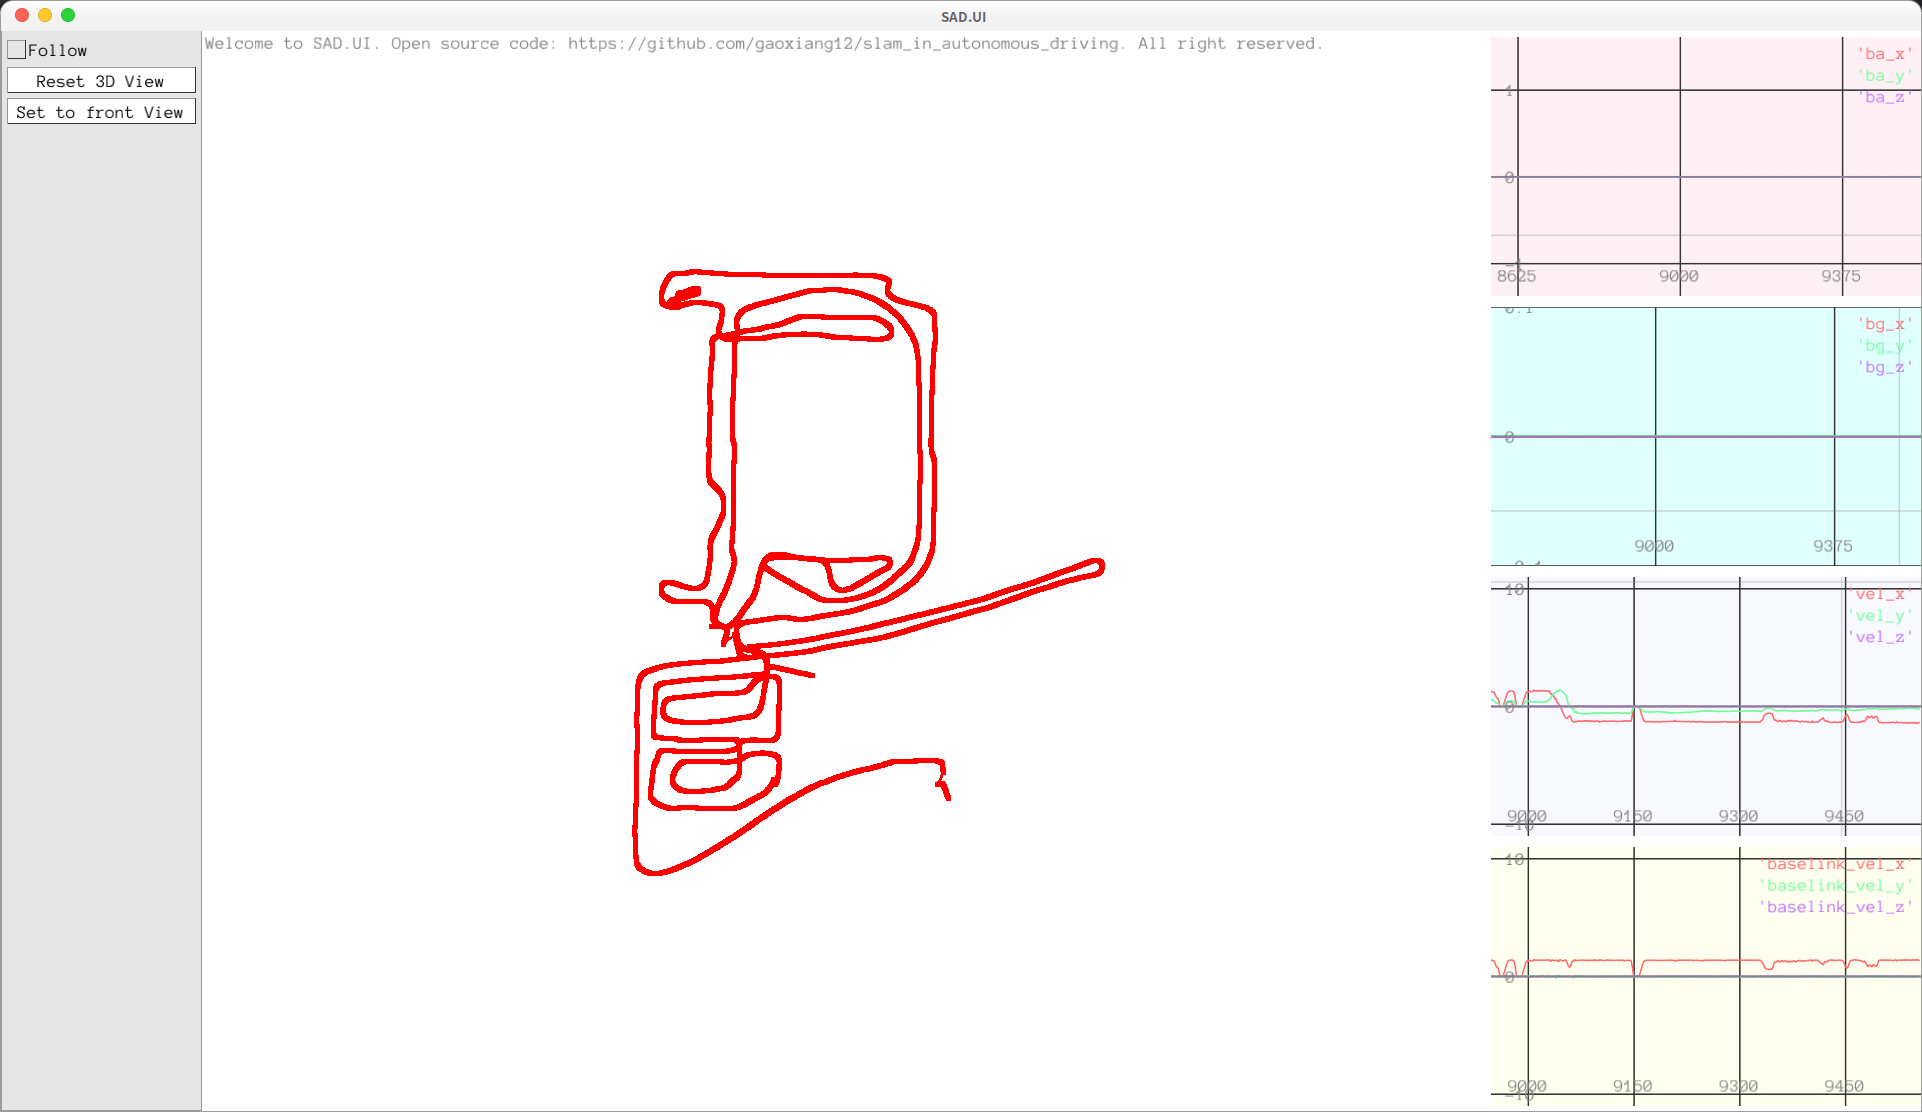
\includegraphics[width=0.8\textwidth]{resources/preintegration/gins-preinteg.png}
	\caption{GINS results based on pre-integration graph optimization}
	\label{fig:gins-preinteg}
\end{figure}

The program will similarly output real-time results and state variable text files. The real-time results are shown in Figure~\ref{fig:gins-preinteg}~, and trajectory results can be plotted using the script from the previous chapter:

\begin{lstlisting}[language=sh,caption=Terminal command:]
	python3 scripts/plot_ch3_state.py ./data/ch4/gins_preintg.txt
\end{lstlisting}

The state diagram is shown in Figure\ref{fig:preintegration-gins}. Overall they are similar to the previous chapter, with velocity states within expected ranges. However, since this chapter's GINS doesn't directly optimize at the Odom level, pure IMU prediction will still diverge locally when GNSS observations are unavailable. Below we discuss the program's approach and its differences from ESKF:

\begin{enumerate}
	\item Compared to ESKF, the pre-integration based graph optimization can accumulate IMU readings. The accumulation duration or number of iterations can be manually selected, while ESKF by default can only iterate once and predict based on single-timestamp IMU data.
	
	\item The pre-integration edge (or called IMU factor/pre-integration factor in factor graph terminology\footnote{This book doesn't distinguish between graph optimization and factor graph concepts, as they are essentially the same in practice. Sometimes we refer to them as \textbf{optimization edges}, other times as \textbf{optimization factors}. Conceptually, \textbf{factor} is more intuitive than \textbf{edge}, so we often discuss various factors while implementing them as edges.}) is a very flexible factor. All six connected vertices can change. To prevent arbitrary state changes, pre-integration factors typically need to be used with other factors. In our case, GNSS factors at both ends constrain pose changes, Odom factors constrain velocity changes, and two bias factors constrain bias variations without limiting absolute bias values.
	
	\item Prior factors make the estimation smoother. Strictly speaking, prior factor covariance matrices should be handled through marginalization. Since this chapter focuses on pre-integration principles, we've set fixed information matrices for prior factors to simplify implementation. In Chapter~\ref{cpt:tightly-lio}~, we'll discuss prior factor information matrix settings and implementation. Readers can try removing this factor to observe its impact on trajectory estimation.
	
	\item Graph optimization conveniently allows setting kernel functions and examining each factor's error contribution, helping identify which parts dominate the optimization. For example, we can analyze normal vs abnormal RTK observation residuals to determine GNSS measurement reliability. Later we'll also introduce how to control optimization flow for more robust results. Readers can enable debug output to examine this information.
	
	\item Due to additional computations, graph optimization is noticeably more time-consuming than filter-based approaches. However, with significant increases in computing power for smart vehicles, graph optimization can now be effectively used in some real-time applications.
\end{enumerate}

\begin{figure}[!t]
	\centering
	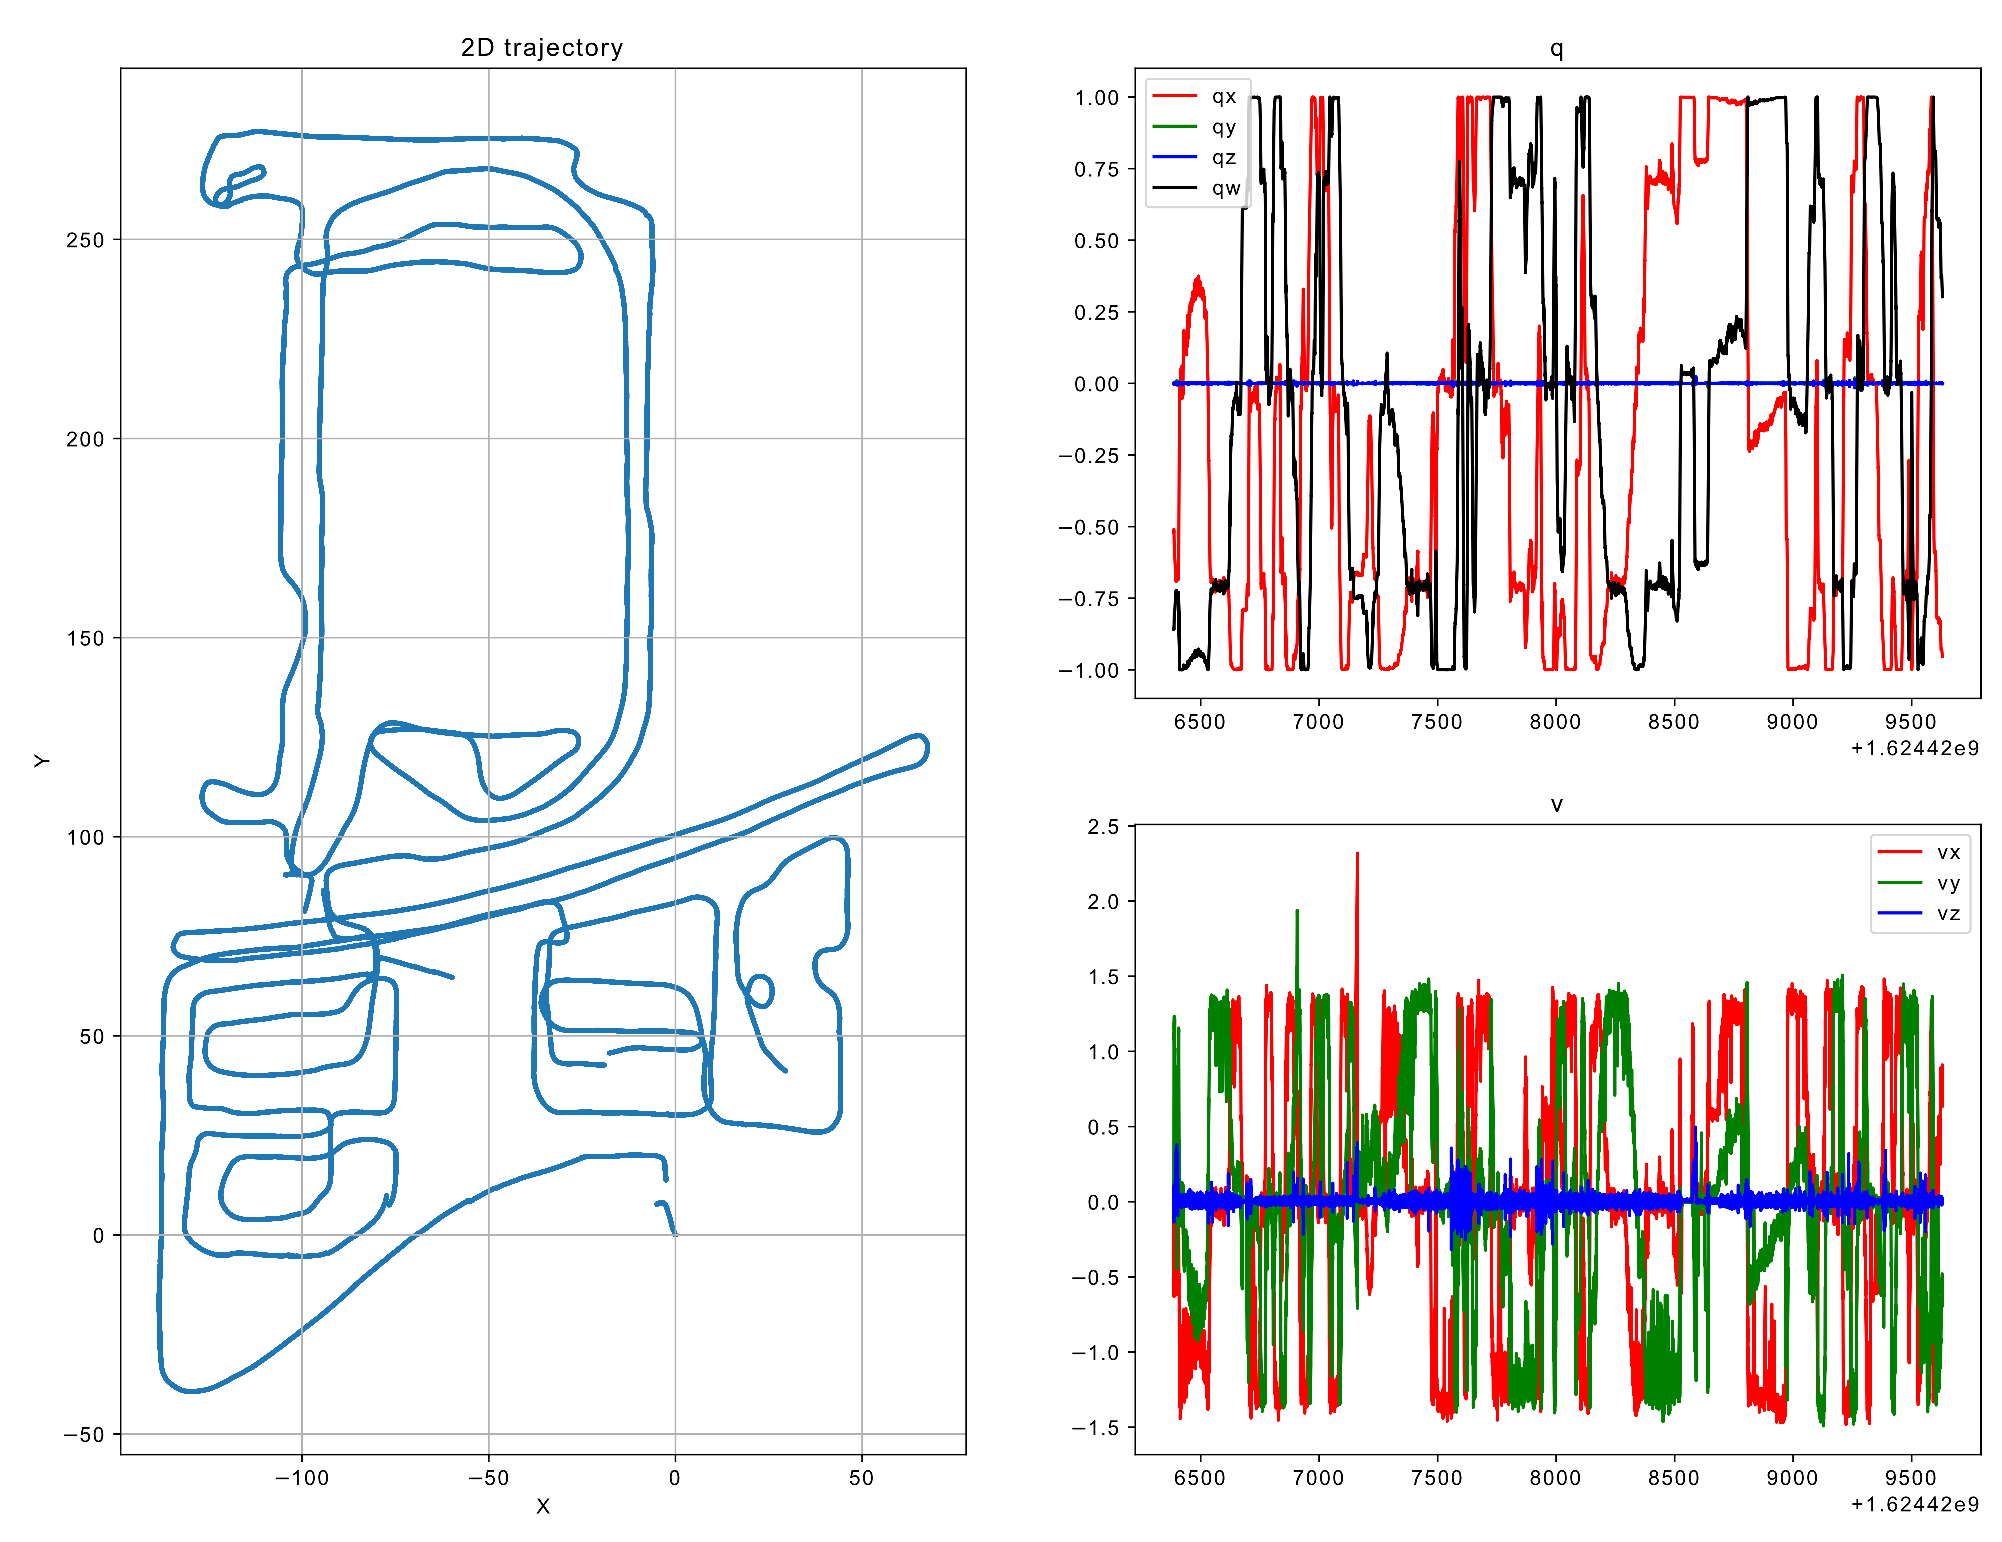
\includegraphics[width=0.8\textwidth]{resources/preintegration/preintegration-gins-out.pdf}
	\caption{GINS results based on pre-integration graph optimization}
	\label{fig:preintegration-gins}
\end{figure}

\section{Summary}
Finally, let's summarize the content of this chapter.

This chapter introduced the fundamental principles of IMU preintegration, including its measurement model, noise model, Jacobian derivation, and handling of biases. Readers can flexibly apply preintegration in practice:

\begin{itemize}
	\item If optimization is not considered, preintegration is completely equivalent to direct integration; it can be used to predict future states.
	\item When used in optimization, preintegration conveniently models the relative motion between two frames. If the IMU bias is fixed, the preintegration model can be greatly simplified. If bias is considered, the preintegrated measurements must be updated accordingly.
	\item The preintegration model can be easily fused with other graph-based optimization models and optimized within the same problem. It also allows flexible configuration of integration time, number of optimized frames, etc., offering more freedom compared to filter-based approaches.
\end{itemize}

Readers are encouraged to compare the content of this chapter with the previous one to understand how two different methods address the same problem. This should be insightful for researchers from various fields.

\section*{Exercises}
\begin{enumerate}
	\item Use numerical differentiation tools to verify the correctness of the Jacobian matrices in preintegration.
	\item Based on the g2o version, implement a Ceres-based version of preintegration DR.
	\item Derive a simplified version of the preintegration model assuming no bias drift. How does it compare to the ESKF approach?
	\item According to the alternative definition in Section~\ref{subsec:4.1.5}, define the preintegration residual, derive its form and Jacobians with respect to each state variable, and discuss whether it offers computational advantages.
	\item Simplify the computation of some Jacobians in preintegration by caching intermediate results to avoid redundant calculations.
	\item In a GINS system based on preintegration, consider how to prevent divergence in position estimates due to prolonged absence of RTK observations. Implement a method to trigger optimization using odometry.
\end{enumerate}



% 5. basic point cloud algorithm
% !Mode:: "TeX:UTF-8"
\part{Laser Localization and Mapping}  
\thispagestyle{empty}  
\chapter{Basic Point Cloud Processing}  
\thispagestyle{empty}  

From this section onwards, we will spend some time introducing the laser SLAM system. Laser sensors are one of the most important sensors in autonomous driving and robotics applications. We can use devices such as lasers, inertial navigation, and satellite navigation to build a complete high-precision mapping and localization application. However, not all researchers are familiar with these sensors. Laser sensors themselves can be categorized into various types, such as single-line, multi-line, mechanical, and solid-state, each with vastly different processing methods.  

In this chapter, we will start with basic point cloud processing algorithms and gradually introduce readers to a complete laser SLAM system, including both 2D and 3D aspects. Compared to inertial navigation data or image data, laser data is relatively simple: lasers only detect the three-dimensional structure of objects and do not involve the kinematics of objects or complex projection processes. Mathematically, a $\mathbb{R}^3$ space can well describe the measurement data from a laser.  

However, at the computational level, we still encounter some issues. The most fundamental of these is \textbf{how to define spatial adjacency}. This problem is referred to as the \textbf{Nearest Neighbour (NN)} problem. We will find that the \textbf{nearest neighbour} between points is the foundation of many algorithms, yet this seemingly simple task can be approached in many different ways computationally. We could use the simplest arrays to represent point clouds, but that would fail to capture the relationships between points. To facilitate adjacency calculations, we also explore more complex \textbf{tree structures}, which are more efficient than traditional methods in handling nearest neighbour problems. Many point cloud registration algorithms require calculating the error between a point and its surrounding points based on some metric. This metric could be the Euclidean distance between points, the \textbf{point-to-line} or \textbf{point-to-plane} distance, or some \textbf{statistically meaningful} metric. Different metric selection methods lead to different algorithms, but they all share common theoretical foundations. For example, pre-dividing space according to some \textbf{criterion} and then building an \textbf{indexed} data structure to facilitate the search for point-to-point adjacency relationships. The methods of division here are diverse, ranging from simple grid-based approaches to planes, spheres, interfaces, etc., giving rise to numerous algorithms. We will introduce the important ones to the readers.  

In this chapter, we will first cover the basic algorithms for point clouds, including how to represent point clouds, how to describe the mathematical model of a laser sensor, how to find the neighbouring points of a given point, how to fit simple geometric shapes to a set of points, and so on. The next two chapters will build upon this content to develop 2D and 3D registration methods.  

\includepdf[width=\textwidth]{art/ch5.pdf}

\section{Mathematical Models of Laser Sensors and Point Clouds}  
\subsection{Mathematical Model of Laser Sensors}  
\begin{figure}[!htp]  
	\centering  
	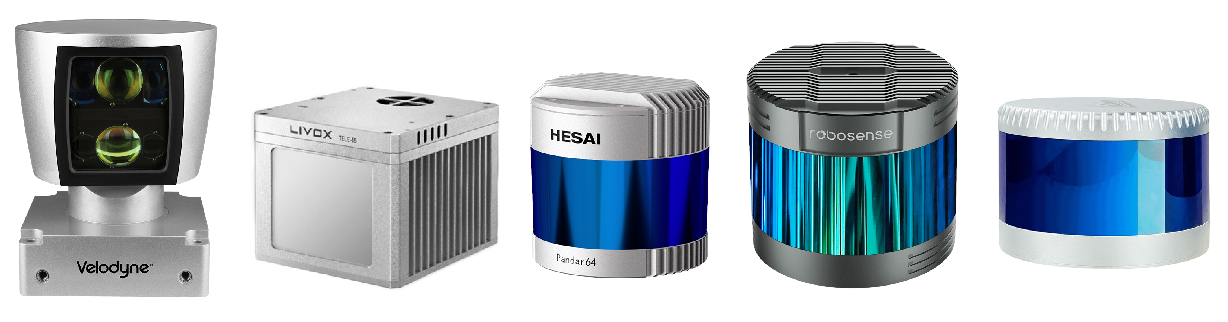
\includegraphics[width=0.8\textwidth]{resources/basic-point-cloud/lidars.pdf}  
	\caption{Various radar models used in autonomous driving. From left to right: Velodyne HDL-64, DJI Livox, Hesai, RoboSense, and LeiShen.}  
	\label{fig:lidars}  
\end{figure}  

Lidar is the most important sensor in autonomous driving. It provides high-precision distance measurement information but remains quite expensive. To this day, there is still intense debate over whether Lidar should be used in autonomous vehicles. Autonomous driving employs various models of Lidar, some of which are listed in Figure~\ref{fig:lidars}. Broadly speaking, Lidar used in autonomous driving can be divided into two types: \textbf{mechanical spinning Lidar} and \textbf{solid-state Lidar}\footnote{Hereafter, we will consistently use the term \textbf{radar} to refer to laser ranging sensors, though this may cause some ambiguity in expression. The \textbf{radar} mentioned here is a transliteration of the English term "Lidar," which stands for Light Detection and Ranging. In the context of autonomous driving, Lidar is often abbreviated as radar. However, in other fields, radar refers to Radio Detection and Ranging, or Radar for short. In Chinese, both Lidar and Radar can be referred to as radar, while in English, they are distinct terms. Notably, autonomous driving also uses millimeter-wave radar, often called Radar. In this book, radar uniformly refers to Lidar, not millimeter-wave radar.}.  

\begin{enumerate}  
	\item \textbf{Mechanical spinning Lidar} can be viewed as a column of laser probes rotating at a fixed frequency. Each probe can quickly measure the distance to external objects.  
	Each full rotation of the probes completes one scan of the surrounding environment. Lidar can be further categorized by the number of lines, common configurations include single-line, 4-line, 8-line, 16-line, 32-line, 64-line, 80-line, and 128-line. The higher the number of lines, the more points are captured per scan, and the richer the information. However, even after multiple price reductions, high-line-count spinning Lidar (32-line and above) remains a very expensive sensor, often costing several times the price of the vehicle itself\footnote{Based on 2021 prices.}.  
	\item \textbf{Solid-state Lidar} is a rapidly developing new type of Lidar in recent years. Unlike mechanical Lidar, solid-state Lidar does not perform 360-degree scans; it can only detect 3D information within a field of view of about 120 degrees. They are very similar to RGB-D cameras (the two are also similar in principle). Most solid-state Lidar systems have a field of view ranging from 60 to 120 degrees but are cheaper and can achieve image-like scanning. In terms of equivalent line count, solid-state Lidar can even achieve effects comparable to 200 lines or more, though solid-state Lidar does not necessarily scan along horizontal lines—some have unique scanning patterns.  
\end{enumerate}  

Spinning Lidar and solid-state Lidar each have their pros and cons. The 360-degree scanning capability of spinning Lidar is highly advantageous for localization and mapping, as the panoramic view ensures that the entire road segment can be mapped in a single pass, and point cloud localization is less susceptible to occlusion. When using solid-state Lidar, multiple units are often combined to achieve a similar panoramic effect. However, spinning Lidar has clear disadvantages in terms of cost and lifespan, and in the near term, it still does not meet automotive-grade or consumer-level price requirements. In contrast, solid-state Lidar can easily achieve costs in the range of several thousand yuan, meeting safety and lifespan requirements at the expense of some field of view (which can be compensated for by using multiple units), and has gained many supporters in recent years. Some high-end vehicle models have already begun equipping solid-state Lidar as part of their perception systems.  

The debate over whether autonomous driving should use Lidar has never ceased. Some believe L4 autonomous driving cannot do without Lidar, while others vehemently argue that Lidar is a burden on vehicles. There are also moderates who are indifferent to the type of sensor, focusing only on functionality and cost. For L4, the early development of autonomous driving primarily relied on mechanical spinning Lidar, so current technical solutions exhibit some degree of path dependence on spinning Lidar. Path dependence refers to the phenomenon where early algorithms and research were tailored to an initial solution, often without regard to cost. Without causing significant issues, there is little incentive to change this solution over time. However, viewed years later, this solution may not necessarily be the best in practice.  

This book does not intend to engage in debates about sensors but focuses solely on introducing their principles and algorithms. Compared to visual and IMU sensors, the measurement of a single laser probe is extremely simple: it merely measures the distance to a point in space, denoted as $r$. Of course, the laser probe itself can be mounted on the vehicle at a certain tilt angle, allowing the spatial position of the endpoint to be determined. This model is called the RAE (Range, Azimuth, Elevation) model, as shown in Figure~\ref{fig:RAE}.  

\begin{figure}[!htp]  
	\centering  
	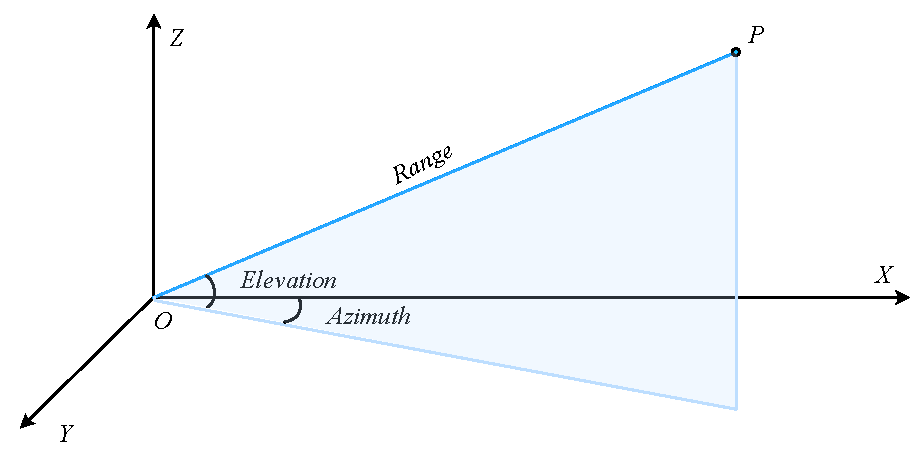
\includegraphics[width=0.8\textwidth]{resources/basic-point-cloud/RAE.pdf}  
	\caption{RAE model for single-point measurement}  
	\label{fig:RAE}  
\end{figure}  

Let the distance be $r=\text{Range}$, the azimuth angle be $A=\text{Azimuth}$, and the elevation angle be $E=\text{Elevation}$. These angles are similar to Euler angles. Based on geometric relationships, the position of $\mathbf{P}$ in the radar reference frame can easily be derived:  
\begin{equation}\label{key}  
	\mathbf{P} = \left[r \cos E \cos A, r \cos E \sin A, r \sin E \right] ^\top.  
\end{equation}  

Conversely, $r, A, E$ can be calculated from $\mathbf{P}=[x,y,z]^\top$:  
\begin{equation}\label{key}  
	\begin{aligned}  
		r &= \sqrt{x^2 + y^2 + z^2}, \\  
		A &= \arctan(y/x), \\  
		E &= \arcsin(z/r).  
	\end{aligned}  
\end{equation}  

These are simply conversions between Euclidean and polar coordinates, with no substantive difference. Spinning Lidar can be viewed as multiple RAE probe models fixed in elevation angle and rotating synchronously in azimuth angle.  
When the probes complete one full rotation, we obtain endpoints with azimuth angles ranging from 0 to 360 degrees. Typically, this set of points is called a \textbf{scan} because it closely resembles the scanning process of a scanner or television. Most Lidar systems can scan the surrounding environment at frequencies of 10 Hz or higher. If such a probe has only one line, it is a single-line Lidar, usually mounted horizontally. Multi-line Lidar can be seen as composed of multiple single-line Lidar units arranged vertically in a column, rotating at a fixed frequency. After one full scan, the multi-line Lidar produces a point cloud that fully reflects the three-dimensional structure within a certain distance. For a single probe, $E$ can be considered fixed, $A$ changes at a constant speed, and only $r$ is derived from actual measurements. This property can be leveraged to compress Lidar data—recording time and distance is simpler than recording Cartesian coordinates (i.e., the $XYZ$ data of the point cloud).  

In addition to distance, Lidar can also carry additional data. For example, multi-line Lidar can record the timestamp, reflectivity, and line number (which line the point belongs to) for each point. This information, particularly reflectivity, can be used in various practical scenarios, such as extracting road markings based on reflectivity or identifying the ground using line numbers. Basic point cloud algorithms, such as nearest neighbor and fitting algorithms, rely solely on Cartesian coordinate position data. Unless otherwise specified, the point clouds discussed hereafter refer to those containing only positional information. However, in visualization, point clouds may be rendered based on height or reflectivity.

\subsection{Representation of Point Clouds}  
\textbf{Point cloud}, in its most literal sense, refers to a set of points scattered in space. The term "\textbf{cloud}" inherently discards the relationships between points. These points are merely Cartesian coordinates in Euclidean space and carry no additional information. Do these points form a mesh? Do certain points constitute a triangle? The point cloud structure does not include such extra details.  

Point clouds are the most fundamental way to represent 3D structures and are the primary data format output by most laser sensors. If we wish to extract additional information from a point cloud, we must employ supplementary data structures to express these relationships. For instance, many algorithms require answering questions like: Which point is the nearest to a given point? What shape do this point and its neighboring points collectively form? To achieve such functionality, additional data structures must be introduced—this is the focus of this section.  

The content of this chapter overlaps with many books on 3D point clouds. Readers may also refer to similar textbooks, such as \cite{Magnusson2009}. As a book aimed at SLAM practitioners, we emphasize point cloud processing for laser sensors rather than discussing generic point cloud processing broadly. We will introduce some usage of the PCL library \cite{Rusu2011}, and for key algorithms, we also provide handwritten implementations along with performance comparisons to their PCL counterparts.  

The simplest and most primitive way to represent a point cloud is as an array: just store the points in an array. This can be easily implemented using `std::vector` in C++. Of course, as mentioned earlier, point clouds can also carry additional information, such as reflectivity, the line number (for multi-line Lidar), or RGB color data. Point clouds from RGB-D cameras may also store the row and column indices of each point in the image. Therefore, a more convenient approach is to define a point cloud structure and use a templated container to store it. If you need to store other information, such as the global position and orientation of the entire point cloud, you can define your own point cloud data structure.  

We illustrate the basics of reading, writing, and visualizing point clouds through a program example, giving readers an intuitive understanding. We have prepared two files for readers: a single-scan point cloud and a map point cloud file, located at `data/ch5/map_example.pcd` and `scan_example.pcd`, respectively. Readers can directly view these files using the `pcl_viewer` command:  
\begin{lstlisting}[language=sh,caption=Terminal input:]  
pcl_viewer ./data/ch5/map_example.pcd  
\end{lstlisting}  

We will also introduce other representation methods later. The example map and scan data are shown in Figure~\ref{fig:pcd-example}. The left point cloud depicts a small "L"-shaped scene consisting of a central building and surrounding greenery, while the right shows data from a single scan. By stitching multiple scans together, we can reconstruct the full map, whereas a single scan clearly contains far fewer points.  

\begin{figure}[!htp]  
	\centering  
	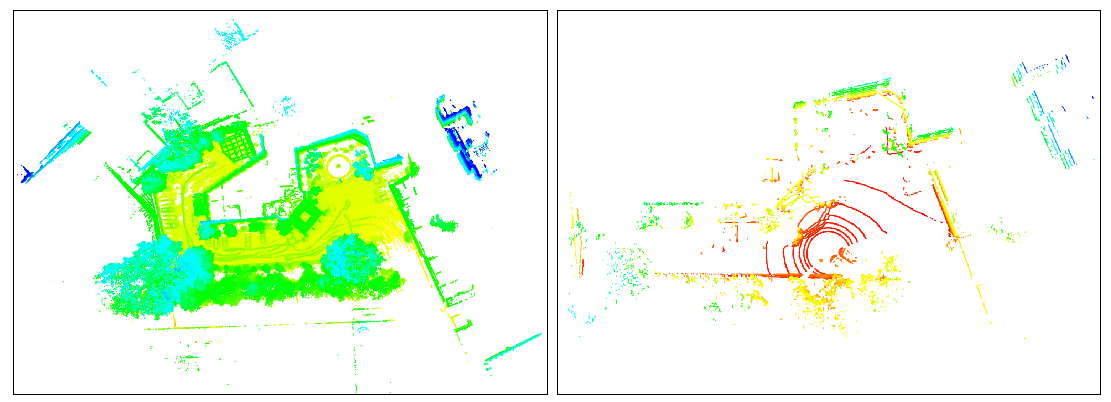
\includegraphics[width=1.0\textwidth]{resources/basic-point-cloud/pcd-example.pdf}  
	\caption{Example data of a point cloud map and a single scan.}  
	\label{fig:pcd-example}  
\end{figure}  

Below, we demonstrate how to read and visualize a point cloud, serving as a basic tutorial for PCL.  
\begin{lstlisting}[language=c++,caption=src/ch5/point\_cloud\_load\_and\_vis.cc]  
int main(int argc, char** argv) {  
	// .. Omitted parameter checking  
	// Load the point cloud  
	PointCloudType::Ptr cloud(new PointCloudType);  
	pcl::io::loadPCDFile(FLAGS_pcd_path, *cloud);  
	
	if (cloud->empty()) {  
		LOG(ERROR) << "cannot load cloud file";  
		return -1;  
	}  
	
	LOG(INFO) << "cloud points: " << cloud->size();  
	
	// Visualize  
	pcl::visualization::PCLVisualizer viewer("cloud viewer");  
	pcl::visualization::PointCloudColorHandlerGenericField<PointType> handle(cloud, "z");  // Color by height  
	viewer.addPointCloud<PointType>(cloud, handle);  
	viewer.spin();  
	
	return 0;  
}  
\end{lstlisting}  

Since data I/O and visualization are handled by existing PCL modules, we only need to call its functions. After compilation, readers can also use the program to view point clouds:  

\begin{lstlisting}[language=sh, caption=Terminal input:]  
bin/point_cloud_load_and_vis --pcd_path ./data/ch5/map_example.pcd  
\end{lstlisting}  

Most programs supporting 3D display can render point clouds effectively. Later, we will continue using 3D graphical interfaces to showcase point cloud registration results.

\subsection{Packet Representation}  

In addition to raw point clouds, there are several other representation methods. Raw point clouds store the coordinates of all points, which consumes significant space. Some representations are more suitable for storage and transmission, while others provide advantageous properties for algorithmic processing. Below, we introduce a few commonly used methods.  

In LiDAR sensors, parameters such as the rotation rate of the radar and the elevation angles of each probe relative to the sensor center are known during the design or operation of the sensor. These are referred to as the \textbf{intrinsic parameters} of the LiDAR. Therefore, these parameters can be stored in a fixed configuration file, while only the runtime-varying measurements need to be recorded in the actual data. For LiDAR, the varying components typically include the detected distance and reflectivity of objects. Leveraging this property can significantly reduce the data transmission volume between the sensor and the computer. Similarly, when storing raw point cloud data, this approach can be used to save disk space instead of storing the full point cloud. This is the concept behind \textbf{data packets} (Packets).  

Most LiDAR manufacturers define their own packet formats, which vary in implementation. These packets can be transmitted and received via various communication protocols (usually network protocols such as UDP). Taking the Velodyne HDL-64S3 as an example (Figure~\ref{fig:packets-example}), let’s examine how hardware manufacturers compress point cloud data.  

\begin{figure}[!htp]  
	\centering  
	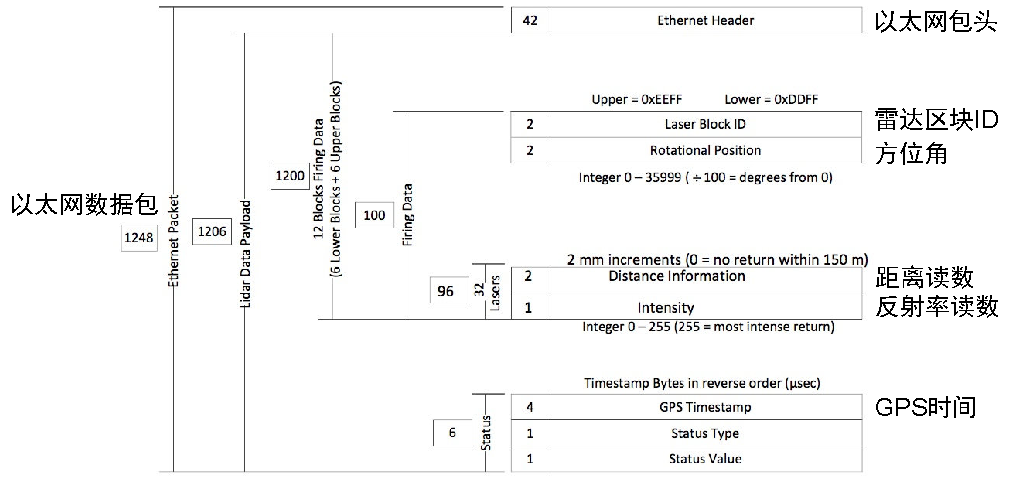
\includegraphics[width=0.8\textwidth]{resources/basic-point-cloud/packets.pdf}  
	\caption{Packet format definition for the Velodyne HDL-64S3}  
	\label{fig:packets-example}  
\end{figure}  

In the Velodyne HDL-64S3, the distance and reflectivity measurements are stored in 3 bytes, while readings from the same column share an azimuth angle and block ID. As shown, 32 readings occupy 100 bytes in total. If stored in PCL format, the positional coordinates and reflectivity of 32 scan lines would require $32 \times (4 + 4 + 4 + 1) = 416$ bytes. Clearly, storing packets is far more efficient than storing raw point clouds.  

However, in many algorithmic implementations, direct access to the coordinates of each point is often preferred. Therefore, packets are typically used as compressed data in modules such as driver software, raw sensor data handling, or map compression. Due to the variety of LiDAR brands and their differing driver implementations, manufacturers usually provide SDKs to handle the conversion between packets and point clouds. Here, we will not delve into the specifics of how each LiDAR compresses and decompresses its data.

\subsection{Bird's-Eye View and Range Image}  
Bird's-eye view (BEV) is another commonly used representation for maps, especially in outdoor environments. If we wish to express LiDAR point clouds in a grid-based format and apply grid-based algorithms for path planning, obstacle avoidance, or 2D annotations, it becomes necessary to represent the point cloud map from a top-down perspective. Of course, converting 3D information to 2D typically involves discarding some data—in this case, the height information of the point cloud.  

Since vehicles are usually horizontally positioned, the sensors mounted on them are also typically level. Under this assumption, converting an outdoor point cloud map to a bird's-eye view is straightforward, as the $x, y, z$ coordinates of the point cloud correspond directly to horizontal and vertical axes. For sensors with tilted or rotating configurations, additional ground or world coordinate system information is required. Below, we convert the point cloud from Figure~\ref{fig:pcd-example} into a bird's-eye view. The BEV is implemented using OpenCV as a 2D image. To map point cloud coordinates to image coordinates, we define a resolution $r$, which determines how many meters each pixel represents. Additionally, we ensure the image center aligns with the point cloud center, while the image dimensions depend on the $x, y$ range of the point cloud.  

Let the point cloud center be $\mathbf{c}=[c_x, c_y]^\top$ and the image center be $I_x, I_y$. A point with coordinates $(x, y, z)$ should map to image coordinates $(u, v)$ as follows:  

\begin{equation}\label{key}  
	\left\{  
	\begin{array}{ll}  
		u &= (x-c_x)/r + I_x, \\  
		v &= (y-c_y)/r + I_y.  
	\end{array}\right.  
\end{equation}  

The $z$-coordinate can then be represented using different colors to indicate height variations. The implementation of this process is shown below:  

\begin{lstlisting}[language=c++,caption=src/ch5/pcd\_to\_bird\_eye.cc]  
DEFINE_string(pcd_path, "./data/ch5/map_example.pcd", "Point cloud file path");  
DEFINE_double(image_resolution, 0.1, "BEV resolution");  
DEFINE_double(min_z, 0.2, "Minimum height for BEV");  
DEFINE_double(max_z, 2.5, "Maximum height for BEV");  

void GenerateBEVImage(PointCloudType::Ptr cloud) {  
	// Compute point cloud boundaries  
	auto minmax_x = std::minmax_element(cloud->points.begin(), cloud->points.end(),  
	[](const PointType& p1, const PointType& p2) { return p1.x < p2.x; });  
	auto minmax_y = std::minmax_element(cloud->points.begin(), cloud->points.end(),  
	[](const PointType& p1, const PointType& p2) { return p1.y < p2.y; });  
	double min_x = minmax_x.first->x;  
	double max_x = minmax_x.second->x;  
	double min_y = minmax_y.first->y;  
	double max_y = minmax_y.second->y;  
	
	const double inv_r = 1.0 / FLAGS_image_resolution;  
	
	const int image_rows = int((max_y - min_y) * inv_r);  
	const int image_cols = int((max_x - min_x) * inv_r);  
	
	float x_center = 0.5 * (max_x + min_x);  
	float y_center = 0.5 * (max_y + min_y);  
	float x_center_image = image_cols / 2;  
	float y_center_image = image_rows / 2;  
	
	// Generate image  
	cv::Mat image(image_rows, image_cols, CV_8UC3, cv::Scalar(255, 255, 255));  
	
	for (const auto& pt : cloud->points) {  
		int x = int((pt.x - x_center) * inv_r + x_center_image);  
		int y = int((pt.y - y_center) * inv_r + y_center_image);  
		if (x < 0 || x >= image_cols || y < 0 || y >= image_rows || pt.z < FLAGS_min_z || pt.z > FLAGS_max_z) {  
			continue;  
		}  
		
		image.at<cv::Vec3b>(y, x) = cv::Vec3b(227, 143, 79);  
	}  
	
	cv::imwrite("./bev.png", image);  
}  
\end{lstlisting}  

Now run:  
\begin{lstlisting}[caption=Terminal input:]  
bin/pcd_to_bird_eye --pcd_path ./data/ch5/map_example.pcd  
\end{lstlisting}  

We assume the point cloud is horizontally aligned and map the $X$ and $Y$ axes to the image. The initial part of the code determines the image boundaries, and then each point's position in the image is calculated based on the specified resolution. Obstacles within a certain height range (here, 0.2 to 2.5 meters, adjustable based on vehicle height) are considered valid and projected onto the BEV, resulting in the output shown in Figure~\ref{fig:bev-example}.  

\begin{figure}[!htp]  
	\centering  
	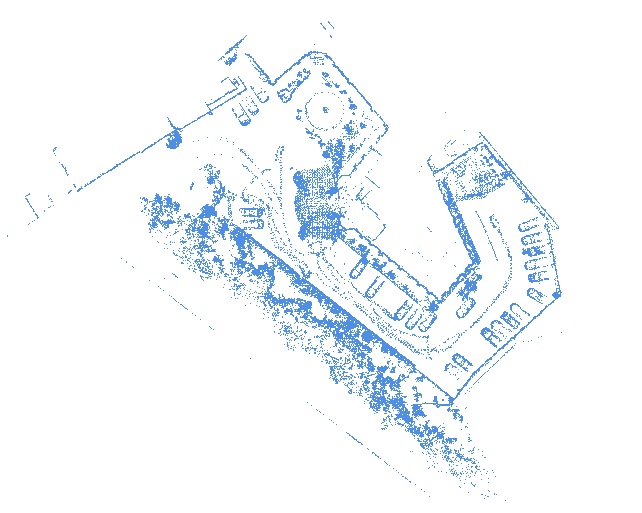
\includegraphics[width=0.6\textwidth]{resources/basic-point-cloud/bev.pdf}  
	\caption{Converting a point cloud to a bird's-eye view}  
	\label{fig:bev-example}  
\end{figure}  

Many path-planning algorithms, such as A* and D* \cite{Delling2009}, operate on grid maps, while perception or obstacle-avoidance algorithms can also use grid maps as input \cite{Sabe2004}. As seen, most obstacle information is preserved when converting point clouds to grid maps, though dynamic objects may leave smearing effects. We will discuss the probabilistic mechanism of grid maps in the 2D LiDAR SLAM chapter, which effectively mitigates the impact of dynamic objects.  

Some readers might wonder: If point clouds can be projected into a bird's-eye view, can they also be projected from other angles? While BEV is the most intuitive choice for top-down observation, similar logic can be applied to generate front or side views, which are computationally equivalent. However, another useful representation for algorithms is the \textbf{range image}.  

The concept of a range image aligns with that of RGB-D cameras. To ensure consistency between depth and color images, RGB-D cameras project point clouds into the color camera's frame. Similarly, can LiDAR point clouds be projected into a virtual camera? The answer is yes. However, since LiDAR point clouds cover a full 360-degree field of view, the resulting image is panoramic. Here, the horizontal axis represents the LiDAR's azimuth angle, while the vertical axis corresponds to the elevation angle. Alternatively, if the elevation angles for each scan line are known, the \textbf{line number} can serve as the vertical axis. Both methods produce what is known as a range image.  

As before, we provide an example to illustrate the appearance of a range image. While generating range images directly from raw LiDAR data (e.g., using block IDs or azimuth angles from packets) is more efficient, this approach depends on the specific LiDAR model. Our example uses post-processed point clouds, requiring only an additional azimuth angle calculation step.

\subsection{Bird's-Eye View and Range Image}  
Bird's-eye view (BEV) is another commonly used representation for maps, especially in outdoor environments. If we wish to express LiDAR point clouds in a grid-based format and apply grid-based algorithms for path planning, obstacle avoidance, or 2D annotations, it becomes necessary to represent the point cloud map from a top-down perspective. Of course, converting 3D information to 2D typically involves discarding some data—in this case, the height information of the point cloud.  

Since vehicles are usually horizontally positioned, the sensors mounted on them are also typically level. Under this assumption, converting an outdoor point cloud map to a bird's-eye view is straightforward, as the $x, y, z$ coordinates of the point cloud correspond directly to horizontal and vertical axes. For sensors with tilted or rotating configurations, additional ground or world coordinate system information is required. Below, we convert the point cloud from Figure~\ref{fig:pcd-example} into a bird's-eye view. The BEV is implemented using OpenCV as a 2D image. To map point cloud coordinates to image coordinates, we define a resolution $r$, which determines how many meters each pixel represents. Additionally, we ensure the image center aligns with the point cloud center, while the image dimensions depend on the $x, y$ range of the point cloud.  

Let the point cloud center be $\mathbf{c}=[c_x, c_y]^\top$ and the image center be $I_x, I_y$. A point with coordinates $(x, y, z)$ should map to image coordinates $(u, v)$ as follows:  

\begin{equation}\label{key}  
	\left\{  
	\begin{array}{ll}  
		u &= (x-c_x)/r + I_x, \\  
		v &= (y-c_y)/r + I_y.  
	\end{array}\right.  
\end{equation}  

The $z$-coordinate can then be represented using different colors to indicate height variations. The implementation of this process is shown below:  

\begin{lstlisting}[language=c++,caption=src/ch5/pcd\_to\_bird\_eye.cc]  
DEFINE_string(pcd_path, "./data/ch5/map_example.pcd", "Point cloud file path");  
DEFINE_double(image_resolution, 0.1, "BEV resolution");  
DEFINE_double(min_z, 0.2, "Minimum height for BEV");  
DEFINE_double(max_z, 2.5, "Maximum height for BEV");  

void GenerateBEVImage(PointCloudType::Ptr cloud) {  
	// Compute point cloud boundaries  
	auto minmax_x = std::minmax_element(cloud->points.begin(), cloud->points.end(),  
	[](const PointType& p1, const PointType& p2) { return p1.x < p2.x; });  
	auto minmax_y = std::minmax_element(cloud->points.begin(), cloud->points.end(),  
	[](const PointType& p1, const PointType& p2) { return p1.y < p2.y; });  
	double min_x = minmax_x.first->x;  
	double max_x = minmax_x.second->x;  
	double min_y = minmax_y.first->y;  
	double max_y = minmax_y.second->y;  
	
	const double inv_r = 1.0 / FLAGS_image_resolution;  
	
	const int image_rows = int((max_y - min_y) * inv_r);  
	const int image_cols = int((max_x - min_x) * inv_r);  
	
	float x_center = 0.5 * (max_x + min_x);  
	float y_center = 0.5 * (max_y + min_y);  
	float x_center_image = image_cols / 2;  
	float y_center_image = image_rows / 2;  
	
	// Generate image  
	cv::Mat image(image_rows, image_cols, CV_8UC3, cv::Scalar(255, 255, 255));  
	
	for (const auto& pt : cloud->points) {  
		int x = int((pt.x - x_center) * inv_r + x_center_image);  
		int y = int((pt.y - y_center) * inv_r + y_center_image);  
		if (x < 0 || x >= image_cols || y < 0 || y >= image_rows || pt.z < FLAGS_min_z || pt.z > FLAGS_max_z) {  
			continue;  
		}  
		
		image.at<cv::Vec3b>(y, x) = cv::Vec3b(227, 143, 79);  
	}  
	
	cv::imwrite("./bev.png", image);  
}  
\end{lstlisting}  

Now run:  
\begin{lstlisting}[caption=Terminal input:]  
bin/pcd_to_bird_eye --pcd_path ./data/ch5/map_example.pcd  
\end{lstlisting}  

We assume the point cloud is horizontally aligned and map the $X$ and $Y$ axes to the image. The initial part of the code determines the image boundaries, and then each point's position in the image is calculated based on the specified resolution. Obstacles within a certain height range (here, 0.2 to 2.5 meters, adjustable based on vehicle height) are considered valid and projected onto the BEV, resulting in the output shown in Figure~\ref{fig:bev-example}.  

\begin{figure}[!htp]  
	\centering  
	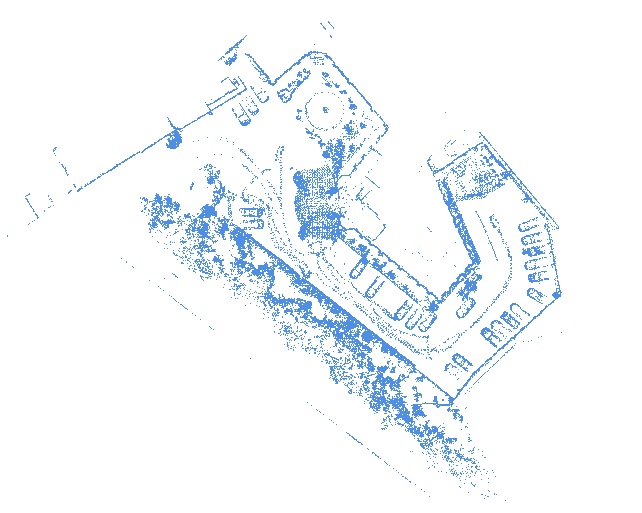
\includegraphics[width=0.6\textwidth]{resources/basic-point-cloud/bev.pdf}  
	\caption{Converting a point cloud to a bird's-eye view}  
	\label{fig:bev-example}  
\end{figure}  

Many path-planning algorithms, such as A* and D* \cite{Delling2009}, operate on grid maps, while perception or obstacle-avoidance algorithms can also use grid maps as input \cite{Sabe2004}. As seen, most obstacle information is preserved when converting point clouds to grid maps, though dynamic objects may leave smearing effects. We will discuss the probabilistic mechanism of grid maps in the 2D LiDAR SLAM chapter, which effectively mitigates the impact of dynamic objects.  

Some readers might wonder: If point clouds can be projected into a bird's-eye view, can they also be projected from other angles? While BEV is the most intuitive choice for top-down observation, similar logic can be applied to generate front or side views, which are computationally equivalent. However, another useful representation for algorithms is the \textbf{range image}.  

The concept of a range image aligns with that of RGB-D cameras. To ensure consistency between depth and color images, RGB-D cameras project point clouds into the color camera's frame. Similarly, can LiDAR point clouds be projected into a virtual camera? The answer is yes. However, since LiDAR point clouds cover a full 360-degree field of view, the resulting image is panoramic. Here, the horizontal axis represents the LiDAR's azimuth angle, while the vertical axis corresponds to the elevation angle. Alternatively, if the elevation angles for each scan line are known, the \textbf{line number} can serve as the vertical axis. Both methods produce what is known as a range image.  

As before, we provide an example to illustrate the appearance of a range image. While generating range images directly from raw LiDAR data (e.g., using block IDs or azimuth angles from packets) is more efficient, this approach depends on the specific LiDAR model. Our example uses post-processed point clouds, requiring only an additional azimuth angle calculation step.  

\begin{lstlisting}[language=c++,caption=src/ch5/scan\_to\_range\_image.cc]
DEFINE_string(pcd_path, "./data/ch5/scan_example.pcd", "Point cloud file path");
DEFINE_double(azimuth_resolution_deg, 0.3, "Azimuth resolution (degrees)");
DEFINE_int32(elevation_rows, 16, "Number of rows for elevation");
DEFINE_double(elevation_range, 15.0, "Elevation range");  // VLP-16 has ±15 degree range
DEFINE_double(lidar_height, 1.128, "LiDAR mounting height");

void GenerateRangeImage(PointCloudType::Ptr cloud) {
	int image_cols = int(360 / FLAGS_azimuth_resolution_deg);  // 360 degrees horizontally divided by resolution
	int image_rows = FLAGS_elevation_rows;                     // Fixed number of rows
	LOG(INFO) << "range image: " << image_rows << "x" << image_cols;
	
	// Create HSV image for better distance visualization
	cv::Mat image(image_rows, image_cols, CV_8UC3, cv::Scalar(0, 0, 0));
	
	double ele_resolution = FLAGS_elevation_range * 2 / FLAGS_elevation_rows;  // Elevation resolution
	
	for (const auto& pt : cloud->points) {
		double azimuth = atan2(pt.y, pt.x) * 180 / M_PI;
		double range = sqrt(pt.x * pt.x + pt.y * pt.y);
		double elevation = atan2((pt.z - FLAGS_lidar_height), range) * 180 / M_PI;
		
		// Normalize azimuth to 0~360
		if (azimuth < 0) {
			azimuth += 360;
		}
		
		int x = int(azimuth / FLAGS_azimuth_resolution_deg);                      // Column
		int y = int((elevation + FLAGS_elevation_range) / ele_resolution + 0.5);  // Row
		
		if (x >= 0 && x < image.cols && y >= 0 && y < image.rows) {
			image.at<cv::Vec3b>(y, x) = cv::Vec3b(uchar(range / 100 * 255.0), 255, 127);
		}
	}
	
	// Flip along Y-axis to make Z-up correspond to image-up
	cv::Mat image_flipped;
	cv::flip(image, image_flipped, 0);
	
	// Convert HSV to RGB
	cv::Mat image_rgb;
	cv::cvtColor(image_flipped, image_rgb, cv::COLOR_HSV2BGR);
	cv::imwrite("./range_image.png", image_rgb);
}
\end{lstlisting}

Several details require attention in this program, such as degree-radian conversion and image flipping along the Y-axis. We use HSV color space to display range information, making distance variations more visually apparent. To convert a single scan to a range image, run:

\begin{lstlisting}[language=sh,caption=Terminal input:]
bin/scan_to_range_image 
\end{lstlisting}

Readers can adjust parameters in gflags to achieve different conversion effects. The converted image is saved as range_image.png in the current directory. With default parameters, since the LiDAR has 16 scan lines, the output will be a long rectangular image of size 1200×16, as shown in Figure~\ref{fig:range-image-example}. The image height can be adjusted by changing the number of elevation rows. This representation resembles camera images but without perspective projection. Some algorithms discussed later will use range images to extract vertical features for localization. Readers can also try identifying ground regions and prominent pole-like objects in this image.

\begin{figure}[!htp]
	\centering
	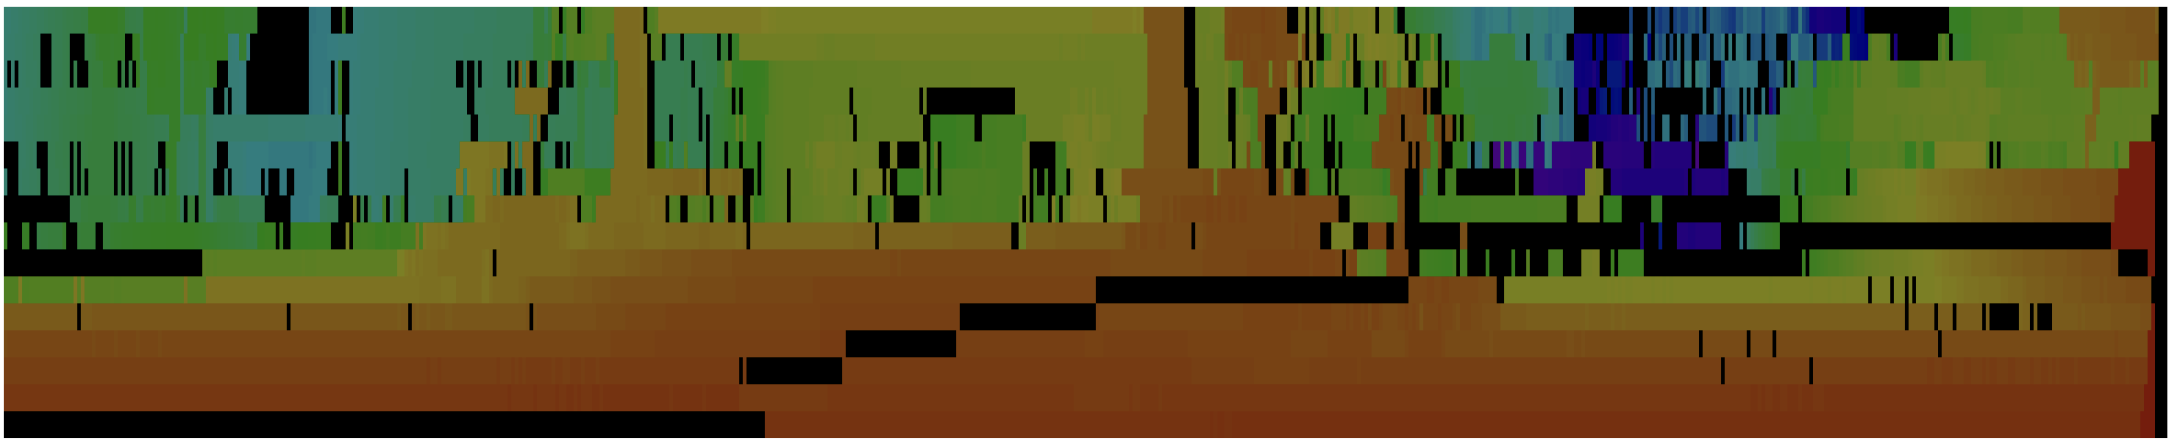
\includegraphics[width=0.8\textwidth]{resources/basic-point-cloud/range-image-raw.png}
	\caption{Converting point cloud to range image. The original range image is hard to display, so we scaled it here.}
	\label{fig:range-image-example}
\end{figure}

\subsection{Alternative Representations}
In addition to the methods previously discussed, some research has applied RGB-D 3D reconstruction techniques to LiDAR point clouds, aiming to achieve better reconstruction quality (and visual effects). For instance, works like \cite{Park2017, Park2018} employ Surfel maps to restore local surface reconstruction effects based on point clouds, while \cite{Roldao2019} demonstrates surface reconstruction using LiDAR data. However, in autonomous driving scenarios, LiDAR's primary functions remain localization and obstacle detection, and these algorithms have yet to become mainstream. We mention these approaches for reference, and interested readers may explore the cited papers.  

Of course, regardless of the representation method, the fundamental measurement data from the LiDAR remains unchanged—it neither becomes artificially denser nor more information-rich. So why use representations like range images or bird's-eye views? The key observation is that while these methods do not alter the raw measurements, they fundamentally change the \textbf{neighborhood relationships between points}. In raw point clouds, the adjacency between points is not explicitly encoded. In contrast, bird's-eye views and range images inherently encode pixel-to-pixel spatial relationships, enabling image-based processing.  

For example, a vertical pillar in 3D space is distributed along the $Z$-axis, but in a range image, it appears as a feature along the $Y$-axis, while in a bird's-eye view, it collapses to a single point. This shift in distribution affects the performance of clustering or feature extraction algorithms. Consequently, some algorithms prefer to extract features from range images or bird's-eye views first, then compute their corresponding 3D positions.

\section{Nearest Neighbor Problem}
The nearest neighbor problem is one of the most fundamental issues in point cloud processing and a step that will be repeatedly invoked in many matching algorithms. The problem can be described very simply: Given a point cloud $\mathcal{X} = \{ \mathbf{x}_1, \ldots, \mathbf{x}_n\}$ containing $n$ points, we ask, which point is closest to a given point $\mathbf{x}_m$? Further, what are the $k$ nearest points to it? Or which points lie within a fixed range $r$ of it? The former is called $k$-nearest neighbor search (kNN), while the latter is called range search.  

Although this problem appears simple, solving it is not trivial, and there are many different approaches. We are particularly concerned with the efficiency of solving the nearest neighbor problem because this algorithm is typically invoked thousands or even millions of times. A small increase in computation time per call can lead to significant efficiency differences in the overall matching algorithm. Below, we introduce nearest neighbor methods in order of increasing complexity, which also aligns with the historical development of algorithmic techniques.  

The algorithms in this chapter will emphasize parallelization, as point cloud algorithms require nearest neighbor searches on a large number of points, making parallel performance a critical consideration.  

\subsection{Brute-Force Nearest Neighbor Search}  
The brute-force nearest neighbor search (BF search) is the simplest and most intuitive method, requiring no auxiliary data structures\footnote{Sometimes referred to as linear search \cite{Weber1998}.} \cite{Kuang2009}. If we search for the nearest neighbor (NN) of a point, we call it \textbf{brute-force nearest neighbor search}; if we search for the $k$ nearest neighbors, we call it brute-force $k$-nearest neighbor search. Overall, this is a straightforward but computationally intensive approach.  

\begin{mdframed}
	\paragraph{Brute-Force Nearest Neighbor Search}  
	Given a point cloud $\mathcal{X}$ and a query point $\mathbf{x}_m$, compute the distance between $\mathbf{x}_m$ and every point in $\mathcal{X}$, then return the minimum distance.  
\end{mdframed}  

Similarly, the brute-force $k$-nearest neighbor search can be defined as:  

\begin{mdframed}
	\paragraph{Brute-Force $k$-Nearest Neighbor (BF kNN)}  
	\begin{enumerate}
		\item For a given point cloud $\mathcal{X}$ and query point $\mathbf{x}_m$, compute the distance between $\mathbf{x}_m$ and every point in $\mathcal{X}$.  
		\item Sort the results from step 1.  
		\item Select the $k$ nearest points.  
		\item Repeat steps 1–3 for all $\mathbf{x}_m$.  
	\end{enumerate}
\end{mdframed}  

Alternatively, we can maintain only the top $k$ results during computation, comparing each new distance with the existing ones to save storage space.  

It is clear that the brute-force method requires traversing the entire point cloud each time. For a point cloud of size $n$, its complexity is $O(n)$. When dealing with the matching problem between two point clouds (assuming both have $n$ points), the complexity of brute-force nearest neighbor search becomes $O(n^2)$. This is obviously a time-consuming method, and BF kNN also requires an additional sorting step. However, the computation for each point in BF search is very simple and does not rely on complex data structures, making it highly parallelizable. A GPU-accelerated BF search or BF kNN may outperform some more sophisticated algorithms \cite{Garcia2008, Li2015}. In most engineering applications, it is also unnecessary to search the entire target point cloud $\mathcal{X}$—instead, searches can be restricted to a predefined local region. Therefore, BF search remains highly practical in many real-world applications.  

To facilitate comparison, we will use a pair of example point clouds (see data/ch5/first.pcd and second.pcd) as data sources in this section, applying various methods to compute their nearest neighbors. Considering that readers may not have access to GPUs, we provide both single-threaded and multi-threaded CPU implementations of nearest neighbor search. Subsequent algorithms will also compare the efficiency of single-threaded versus multi-threaded implementations. For simpler methods (such as the BF method in this section), we will also compare handwritten implementations with those provided by the PCL library.

\subsubsection{Brute-Force Nearest Neighbor Implementation}
The BF (Brute-Force) matching implementation is straightforward. Using C++17's parallel mechanisms, it's easy to extend the single-threaded version to a multi-threaded one. We utilize STL algorithms to implement both single-threaded and multi-threaded BF matching, first defining a brute-force nearest neighbor search for a single point and then extending it to compute nearest neighbors for multiple points.

\begin{lstlisting}[language=c++, caption=src/ch5/bfnn.cc]
int bfnn_point(CloudPtr cloud, const Vec3f& point) {
	return std::min_element(cloud->points.begin(), cloud->points.end(),
		[&point](const PointType& pt1, const PointType& pt2) -> bool {
			return (pt1.getVector3fMap() - point).squaredNorm() <
			(pt2.getVector3fMap() - point).squaredNorm();
		}) - cloud->points.begin();
}

void bfnn_cloud_mt(CloudPtr cloud1, CloudPtr cloud2, std::vector<std::pair<size_t, size_t>>& matches) {
	// Generate indices first
	std::vector<size_t> index(cloud1->size());
	std::for_each(index.begin(), index.end(), [idx = 0](size_t& i) mutable { i = idx++; });
	
	// Parallel for_each
	matches.resize(index.size());
	std::for_each(std::execution::par_unseq, index.begin(), index.end(), [&](auto idx) {
		matches[idx].second = idx;
		matches[idx].first = bfnn_point(cloud1, ToVec3f(cloud2->points[idx]));
	});
}
\end{lstlisting}

In the single-point nearest neighbor search, we take a point as input, compute the distance to every point in the cloud, and then retrieve the minimum. This is achieved using `std::min_element` and a lambda function. The parallel version uses `std::execution` to concurrently invoke the single-point nearest neighbor algorithm for each point.

Next, let's examine the test program. This section uses gtest to benchmark various nearest neighbor methods for comparison:

\begin{lstlisting}[language=c++,caption=src/ch5/test\_nn.cc]
TEST(CH5_TEST, BFNN) {
	sad::CloudPtr first(new sad::PointCloudType), second(new sad::PointCloudType);
	pcl::io::loadPCDFile(FLAGS_first_scan_path, *first);
	pcl::io::loadPCDFile(FLAGS_second_scan_path, *second);
	
	if (first->empty() || second->empty()) {
		LOG(ERROR) << "cannot load cloud";
		FAIL();
	}
	
	// Apply voxel grid downsampling to 0.05
	sad::VoxelGrid(first);
	sad::VoxelGrid(second);
	
	// Benchmark single-threaded and multi-threaded brute-force matching
	sad::evaluate_and_call(
	[&first, &second]() {
		std::vector<std::pair<size_t, size_t>> matches;
		sad::bfnn_cloud(first, second, matches);
	},
	"Brute-Force Matching (Single-threaded)", 5);
	sad::evaluate_and_call(
	[&first, &second]() {
		std::vector<std::pair<size_t, size_t>> matches;
		sad::bfnn_cloud_mt(first, second, matches);
	},
	"Brute-Force Matching (Multi-threaded)", 5);
	
	SUCCEED();
}
\end{lstlisting}

Here, the `evaluate_and_call` function is used. This function invokes a specified method a fixed number of times and measures its execution time:
\begin{lstlisting}[language=c++,caption=src/common/sys\_utils.h]
/**
* Measure code execution time
* @tparam FuncT
* @param func  Function to be called
* @param func_name  Function name
* @param times  Number of calls
*/
template <typename FuncT>
void evaluate_and_call(FuncT func, const std::string &func_name = "", int times = 10) {
	double total_time = 0;
	for (int i = 0; i < times; ++i) {
		auto t1 = std::chrono::high_resolution_clock::now();
		func();
		auto t2 = std::chrono::high_resolution_clock::now();
		total_time += std::chrono::duration_cast<std::chrono::duration<double>>(t2 - t1).count() * 1000;
	}
	
	LOG(INFO) << "Method " << func_name << " average call time/iterations: " << total_time / times << "/" << times << " ms.";
}
\end{lstlisting}

We call both the single-threaded and multi-threaded versions five times each and compute their average execution times.

\begin{lstlisting}[language=sh,caption=Terminal output]
bin/test_nn --gtest_filter=CH5_TEST.BFNN 
Note: Google Test filter = CH5_TEST.BFNN
[==========] Running 1 test from 1 test suite.
[----------] Global test environment set-up.
[----------] 1 test from CH5_TEST
[ RUN      ] CH5_TEST.BFNN
Failed to find match for field 'intensity'.
Failed to find match for field 'intensity'.
I0116 13:40:57.001132 267085 test_nn.cc:36] points: 18869, 18779
I0116 13:41:04.886138 267085 sys_utils.h:32] Method Brute-Force Matching (Single-threaded) average call time/iterations: 1576.98/5 ms.
I0116 13:41:05.291601 267085 sys_utils.h:32] Method Brute-Force Matching (Multi-threaded) average call time/iterations: 81.0873/5 ms.
\end{lstlisting}

As shown, for point clouds with around 18,000 points, the single-threaded brute-force matching takes approximately 1.5 seconds, while the multi-threaded version requires only 81 milliseconds. These benchmarks are highly dependent on machine performance. The tests were conducted on an i9-12900KF machine, and readers may observe different results (possibly significant variations) on their own systems. However, the relative speed differences between algorithms remain consistent for evaluation purposes. 

The advantage of brute-force matching is that it computes matches for every pair of points, ensuring correctness. Subsequent methods may not guarantee this. We now use brute-force matching results as a benchmark to evaluate the performance of other approaches.

\subsection{Grid and Voxel Methods}
Brute-force search (or linear search) essentially involves traversing and searching through a data structure. Students familiar with data structures would immediately suggest that for sorted containers, binary search is clearly faster than sequential search. With a bit more recall, one might remember that binary search reduces the complexity to \(O(\log_2 N)\) compared to linear search. This line of thinking leads to the binary trees and K-d trees discussed in Section~\ref{sec:binary-tree}. Tree structures index the data itself. On the other hand, since point clouds are spatial data, we can also index them spatially. Depending on the indexing method, this leads to 2D grid or 3D voxel approaches, and further to quadtrees and octrees. This section focuses on the latter category.

\begin{figure}[!htp]
	\centering
	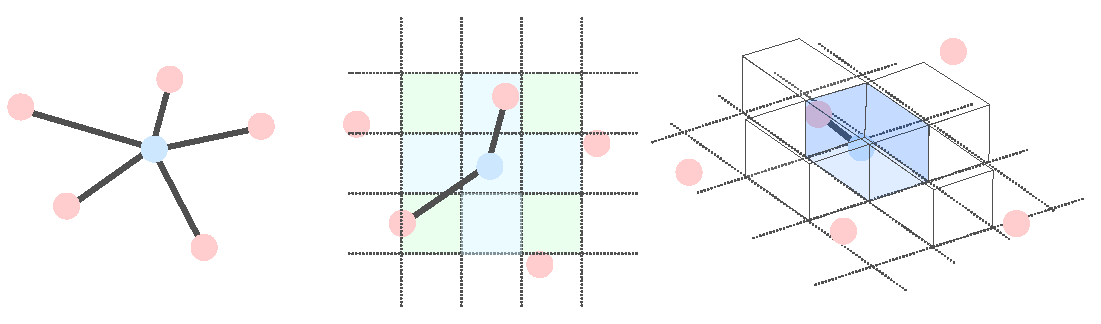
\includegraphics[width=0.8\textwidth]{resources/basic-point-cloud/grid-and-voxel.pdf}
	\caption{Nearest neighbor search: grid and voxel methods. In the grid method, space is divided into 2D projected grids, and the nearest points are searched within the surrounding grids of the query point. In voxel-based methods, space is divided into 3D voxels, and the search is performed in adjacent voxels. For simplicity, only four surrounding voxels are shown here; in practice, the top and bottom voxels should also be included, totaling six.}
	\label{fig:grid-and-voxel}
\end{figure}

\subsubsection{Grid-Based Nearest Neighbor Search}
If we partition the point cloud spatially into grids, we can compute the grid position for each point and index all points spatially, as shown in Figure~\ref{fig:grid-and-voxel}. When searching for the nearest neighbor, we first compute the grid cell containing the query point and then search for its nearest neighbor in the surrounding grid cells. The nearest neighbor in the grid can be easily defined, such as the adjacent cells above, below, left, and right, significantly narrowing the search scope. However, there are a few considerations when generating the grid:

\begin{itemize}
	\item Based on the density of the point cloud, we need to predefine the \textbf{resolution} of the grid, which is a \textbf{hyperparameter}—a parameter related to the computational task. If the grid cells are too large, each cell will contain many points, reducing the efficiency of nearest neighbor search. If the cells are too small, the number of cells increases, and due to the sparsity of the point cloud, the nearest neighbor might not lie in the adjacent cells, potentially missing the true nearest neighbor. This method is highly sensitive to \textbf{hyperparameters} and requires empirical tuning.
	\item Since grid boundaries are discrete, when searching for the nearest neighbor, we should not only search within the current grid cell but also in its \textbf{surrounding} cells. The definition of \textbf{surrounding} can vary. For 2D grids, we might consider the four adjacent cells (up, down, left, right) as "surrounding," or include the four corners for a total of eight cells. Clearly, the more surrounding cells included, the more cells need to be searched, reducing algorithmic efficiency. Thus, a reasonable value must be chosen in practice. This issue also applies to voxel methods, where we can similarly define six adjacent voxels or include the eight corners for a total of 14 neighboring voxels.
	\item Due to the limited scope of grid searches, it is possible to fail to find the nearest neighbor for a given point. This is quite different from brute-force search, which can match all points and thus guarantees finding the nearest neighbor for every point. Grid methods, however, do not always guarantee this. Therefore, in addition to evaluating the computational efficiency of grid methods, their \textbf{correctness} must also be assessed. The same applies to subsequent algorithms.
\end{itemize}

\subsubsection{Voxel-Based Nearest Neighbor Search}
Voxel-based nearest neighbor search is very similar to the grid method. While the grid method partitions space into 2D grids, the voxel method divides space into 3D \textbf{voxels}—think of them as small cubes forming a partitioning scheme. A voxel is directly adjacent to six surrounding voxels; including diagonals adds another eight, for a total of 14 adjacent voxels.

\subsubsection{Implementation}
Since 2D grids and voxel methods are very similar, we implement them using a template class. We use the dimensionality as a template parameter and employ 2D or 3D integer vectors as grid indices to unify the implementation of 2D and 3D grids, keeping the code as compact as possible. Additionally, we define neighboring relationships through enumerations, allowing users to specify the desired adjacency type.

First, let's look at the basic definition of grid-based nearest neighbor search:
\begin{lstlisting}[language=c++,caption=src/ch5/gridnn.hpp]
/**
* Grid-based nearest neighbor search
* @tparam dim Template parameter, using 2D or 3D voxels
*/
template <int dim>
class GridNN {
	public:
	using KeyType = Eigen::Matrix<int, dim, 1>;
	using PtType = Eigen::Matrix<float, dim, 1>;
	
	enum class NearbyType {
		CENTER,  // Only consider the center
		// For 2D
		NEARBY4,  // Up, down, left, right
		NEARBY8,  // Up, down, left, right + four corners
		
		// For 3D
		NEARBY6,  // Up, down, left, right, front, back
	};
	
	private:
	float resolution_ = 0.1;       // Resolution
	float inv_resolution_ = 10.0;  // Inverse of resolution
	
	NearbyType nearby_type_ = NearbyType::NEARBY4;
	std::unordered_map<KeyType, std::vector<size_t>, hash_vec<dim>> grids_;  // Grid data
	CloudPtr cloud_;
	
	std::vector<KeyType> nearby_grids_;  // Nearby grids
};
\end{lstlisting}

We define neighboring relationships as the enumeration type `NearbyType`, and the actual grid data is stored in an `std::unordered_map` (hash table). Since point clouds are sparse, the corresponding grids are also sparse, so empty grids need not be retained where no data exists. Hash tables are highly effective in this application scenario. We define the key of this table as a 2D or 3D integer vector and implement the hash function as follows:

\begin{lstlisting}[language=c++,caption=src/common/eigen\_types.h]
/// Vector hash
template <int N>
struct hash_vec {
	inline size_t operator()(const Eigen::Matrix<int, N, 1>& v) const;
};

template <>
inline size_t hash_vec<2>::operator()(const Eigen::Matrix<int, 2, 1>& v) const {
	return size_t(((v[0] * 73856093) ^ (v[1] * 471943)) % 10000000);
}

template <>
inline size_t hash_vec<3>::operator()(const Eigen::Matrix<int, 3, 1>& v) const {
	return size_t((v[0] * 73856093) ^ (v[1] * 471943) ^ (v[2] * 83492791) % 10000000);
}
\end{lstlisting}

The `hash_vec` function is a template function with two specializations for 2D and 3D spatial hash functions, respectively. According to the literature \cite{Teschner2003}, spatial hash functions can be implemented by multiplying each dimension's data by a large prime number, then taking the XOR, and finally applying modulo with a large integer. For a spatial point \(\mathbf{p}=[p_x, p_y, p_z]\), using three large prime numbers \(n_1, n_2, n_3\) and a large integer \(N\), its hash function can be defined as:
\begin{equation}\label{key}
	\text{hash}(\mathbf{p}) = ((p_x n_1) ~ \mathrm{xor}~ (p_y n_2) ~\mathrm{xor}~ (p_z n_3))~\text{mod}~ N.
\end{equation}

Similarly, we can define a hash function for 2D spatial points. Combined with the template parameter `dim` of the `GridNN` class, these can be used as implementations for the hash function in `std::unordered_map`. Then, we define their nearest neighbors in the `nearby_grids_` member variable:

\begin{lstlisting}[language=c++,caption=src/ch5/gridnn.hpp]
template <>
void GridNN<2>::GenerateNearbyGrids() {
	if (nearby_type_ == NearbyType::CENTER) {
		nearby_grids_.emplace_back(KeyType::Zero());
	} else if (nearby_type_ == NearbyType::NEARBY4) {
		nearby_grids_ = {Vec2i(0, 0), Vec2i(-1, 0), Vec2i(1, 0), Vec2i(0, 1), Vec2i(0, -1)};
	} else if (nearby_type_ == NearbyType::NEARBY8) {
		nearby_grids_ = {
			Vec2i(0, 0),   Vec2i(-1, 0), Vec2i(1, 0),  Vec2i(0, 1), Vec2i(0, -1),
			Vec2i(-1, -1), Vec2i(-1, 1), Vec2i(1, -1), Vec2i(1, 1),
		};
	}
}

template <>
void GridNN<3>::GenerateNearbyGrids() {
	if (nearby_type_ == NearbyType::CENTER) {
		nearby_grids_.emplace_back(KeyType::Zero());
	} else if (nearby_type_ == NearbyType::NEARBY6) {
		nearby_grids_ = {KeyType(0, 0, 0),  KeyType(-1, 0, 0), KeyType(1, 0, 0), KeyType(0, 1, 0),
			KeyType(0, -1, 0), KeyType(0, 0, -1), KeyType(0, 0, 1)};
	}
}
\end{lstlisting}

Using specialized template classes, we can define different neighbor generation methods for 2D and 3D voxels. The 2D grid allows selecting 0, 4, or 8 nearest neighbors, while the 3D voxel allows selecting 0 or 6 nearest neighbors (the 14-neighbor case is left as an exercise for the reader). Now, let's implement the nearest neighbor search logic:
\begin{enumerate}
	\item First, compute the grid cell containing the given point.
	\item Based on the nearest neighbor definition, search the nearby grid cells.
	\item Collect the results from step 2 and use brute-force matching to compute the nearest neighbor within these grid cells.
\end{enumerate}

Step 3 can reuse the brute-force matching code from earlier. This process is the same for both 2D and 3D grids, so we use the same interface at the code level. The single nearest neighbor search function is as follows:

\begin{lstlisting}[language=c++,caption=src/ch5/gridnn.hpp]
template <int dim>
bool GridNN<dim>::GetClosestPoint(const PointType& pt, PointType& closest_pt, size_t& idx) {
	// Search for the nearest neighbor in the grid cells around pt
	std::vector<size_t> idx_to_check;
	auto key = Pos2Grid(ToEigen<float, dim>(pt));
	
	std::for_each(nearby_grids_.begin(), nearby_grids_.end(), [&key, &idx_to_check, this](const KeyType& delta) {
		auto dkey = key + delta;
		auto iter = grids_.find(dkey);
		if (iter != grids_.end()) {
			idx_to_check.insert(idx_to_check.end(), iter->second.begin(), iter->second.end());
		}
	});
	
	if (idx_to_check.empty()) {
		return false;
	}
	
	// Brute-force NN in cloud_[idx]
	idx = bfnn_point(cloud_, idx_to_check, ToVec3f(pt));
	closest_pt = cloud_->points[idx];
	return true;
}

template <int dim>
Eigen::Matrix<int, dim, 1> GridNN<dim>::Pos2Grid(const Eigen::Matrix<float, dim, 1>& pt) {
	return (pt * inv_resolution_).template cast<int>();
}
\end{lstlisting}

The point cloud version simply adds a concurrent wrapper around this function:
\begin{lstlisting}[language=c++,caption=src/ch5/gridnn.hpp]
template <int dim>
bool GridNN<dim>::GetClosestPointForCloudMT(CloudPtr ref, CloudPtr query,
std::vector<std::pair<size_t, size_t>>& matches) {
	// Essentially the same as the serial version, but matches must be preallocated, with invalid matches filled on failure
	std::vector<size_t> index(query->size());
	std::for_each(index.begin(), index.end(), [idx = 0](size_t& i) mutable { i = idx++; });
	matches.resize(index.size());
	
	std::for_each(std::execution::par_unseq, index.begin(), index.end(), [this, &matches, &query](const size_t& idx) {
		PointType cp;
		size_t cp_idx;
		if (GetClosestPoint(query->points[idx], cp, cp_idx)) {
			matches[idx] = {cp_idx, idx};
		} else {
			matches[idx] = {math::kINVALID_ID, math::kINVALID_ID};
		}
	});
	
	return true;
}
\end{lstlisting}


Now let's test the performance of various 2D and 3D voxel methods under different nearest neighbor definitions. Note that in addition to testing performance, we should also focus on whether these nearest neighbors are correct. In fact, grid-based nearest neighbor search may encounter two types of errors:

\begin{enumerate}
	\item The nearest neighbor detected by the grid method is not actually the nearest neighbor in reality. This is called a \textbf{false positive} (FP). The number of false positives in an experiment is denoted as \(FP\).
	\item A true nearest neighbor in reality is not detected by the grid method. This is called a \textbf{false negative} (FN). The number of false negatives in an experiment is denoted as \(FN\).
\end{enumerate}

Using the definitions of \(FP\) and \(FN\), we can define the algorithm's \textbf{precision} and \textbf{recall}. Let \(m\) be the total number of nearest neighbors computed by the algorithm and \(n\) be the total number of ground truth nearest neighbors. Then, precision and recall are defined as:
\begin{equation}\label{key}
	\text{precision} = \frac{1-FP}{m}, \quad \text{recall} = \frac{1-FN}{n}
\end{equation}

Precision describes the correctness of the nearest neighbors detected by the algorithm, while recall describes the proportion of true results that the algorithm successfully detects. A well-performing algorithm should achieve high values in both metrics, but this may come at the cost of slower performance. For example, brute-force matching can achieve 100\% precision and recall, but its computational time is often unacceptable.

When testing nearest neighbor algorithms, we can evaluate their precision and recall using the following method:
\begin{lstlisting}[language=c++,caption=src/ch5/test\_nn.cc]
/**
* Evaluate the correctness of nearest neighbor matches
* @param truth Ground truth matches
* @param esti  Estimated matches
*/
void EvaluateMatches(const std::vector<std::pair<size_t, size_t>>& truth,
const std::vector<std::pair<size_t, size_t>>& esti) {
	int fp = 0;  // false-positive: exists in esti but not in truth
	int fn = 0;  // false-negative: exists in truth but not in esti
	
	/// Check if a match exists in another container
	auto exist = [](const std::pair<size_t, size_t>& data, const std::vector<std::pair<size_t, size_t>>& vec) -> bool {
		return std::find(vec.begin(), vec.end(), data) != vec.end();
	};
	
	for (const auto& d : esti) {
		if (!exist(d, truth)) {
			fp++;
		}
	}
	
	for (const auto& d : truth) {
		if (!exist(d, esti)) {
			fn++;
		}
	}
	
	float precision = 1.0 - float(fp) / esti.size();
	float recall = 1.0 - float(fn) / truth.size();
	LOG(INFO) << "precision: " << precision << ", recall: " << recall << ", fp: " << fp << ", fn: " << fn;
}
\end{lstlisting}

Next, we test the grid-based nearest neighbor method:

\begin{lstlisting}[language=c++,caption=src/ch5/test\_nn.cc]
TEST(CH5_TEST, GRID_NN) {
	// Code for loading point clouds omitted
	std::vector<std::pair<size_t, size_t>> truth_matches;
	sad::bfnn_cloud(first, second, truth_matches);
	
	// Compare different types of grids
	sad::GridNN<2> grid0(0.1, sad::GridNN<2>::NearbyType::CENTER), grid4(0.1, sad::GridNN<2>::NearbyType::NEARBY4),
	grid8(0.1, sad::GridNN<2>::NearbyType::NEARBY8);
	sad::GridNN<3> grid3(0.1, sad::GridNN<3>::NearbyType::NEARBY6);
	
	grid0.SetPointCloud(first);
	grid4.SetPointCloud(first);
	grid8.SetPointCloud(first);
	grid3.SetPointCloud(first);
	
	// Evaluate various versions of Grid NN
	
	LOG(INFO) << "===================";
	std::vector<std::pair<size_t, size_t>> matches;
	sad::evaluate_and_call(
	[&first, &second, &grid0, &matches]() { grid0.GetClosestPointForCloud(first, second, matches); },
	"Grid0 Single-threaded", 10);
	EvaluateMatches(truth_matches, matches);
	
	LOG(INFO) << "===================";
	sad::evaluate_and_call(
	[&first, &second, &grid0, &matches]() { grid0.GetClosestPointForCloudMT(first, second, matches); },
	"Grid0 Multi-threaded", 10);
	EvaluateMatches(truth_matches, matches);
	
	/// Other test methods are similar and omitted
}
\end{lstlisting}

We primarily compare the runtime and nearest neighbor performance of each method. Readers should observe the same precision and recall metrics, though runtime may vary.

\begin{lstlisting}[language=sh,caption=Terminal output:]
./bin/test_nn --gtest_filter=CH5_TEST.GRID_NN 
I0116 17:04:58.055471 276361 test_nn.cc:125] ===================
I0116 17:04:58.065711 276361 sys_utils.h:32] Method Grid0 Single-threaded average call time/iterations: 1.02376/10 ms.
I0116 17:04:58.065724 276361 test_nn.cc:65] truth: 18869, esti: 8518
I0116 17:04:58.099488 276361 test_nn.cc:91] precision: 0.486382, recall: 0.219566, fp: 4375, fn: 14726
I0116 17:04:58.099493 276361 test_nn.cc:132] ===================
I0116 17:04:58.104143 276361 sys_utils.h:32] Method Grid0 Multi-threaded average call time/iterations: 0.464818/10 ms.
I0116 17:04:58.104161 276361 test_nn.cc:65] truth: 18869, esti: 18779
I0116 17:04:58.158778 276361 test_nn.cc:91] precision: 0.486382, recall: 0.219566, fp: 4375, fn: 14726
I0116 17:04:58.158783 276361 test_nn.cc:138] ===================
I0116 17:04:58.202162 276361 sys_utils.h:32] Method Grid4 Single-threaded average call time/iterations: 4.33758/10 ms.
I0116 17:04:58.202165 276361 test_nn.cc:65] truth: 18869, esti: 13272
I0116 17:04:58.246877 276361 test_nn.cc:91] precision: 0.646775, recall: 0.454926, fp: 4688, fn: 10285
I0116 17:04:58.246881 276361 test_nn.cc:144] ===================
I0116 17:04:58.254035 276361 sys_utils.h:32] Method Grid4 Multi-threaded average call time/iterations: 0.715278/10 ms.
I0116 17:04:58.254041 276361 test_nn.cc:65] truth: 18869, esti: 18779
I0116 17:04:58.308115 276361 test_nn.cc:91] precision: 0.646775, recall: 0.454926, fp: 4688, fn: 10285
I0116 17:04:58.308118 276361 test_nn.cc:150] ===================
I0116 17:04:58.379315 276361 sys_utils.h:32] Method Grid8 Single-threaded average call time/iterations: 7.11945/10 ms.
I0116 17:04:58.379319 276361 test_nn.cc:65] truth: 18869, esti: 14613
I0116 17:04:58.425294 276361 test_nn.cc:91] precision: 0.728735, recall: 0.564365, fp: 3964, fn: 8220
I0116 17:04:58.425297 276361 test_nn.cc:156] ===================
I0116 17:04:58.433573 276361 sys_utils.h:32] Method Grid8 Multi-threaded average call time/iterations: 0.827275/10 ms.
I0116 17:04:58.433579 276361 test_nn.cc:65] truth: 18869, esti: 18779
I0116 17:04:58.485752 276361 test_nn.cc:91] precision: 0.728735, recall: 0.564365, fp: 3964, fn: 8220
I0116 17:04:58.485755 276361 test_nn.cc:162] ===================
I0116 17:04:58.513800 276361 sys_utils.h:32] Method Grid 3D Single-threaded average call time/iterations: 2.80424/10 ms.
I0116 17:04:58.513803 276361 test_nn.cc:65] truth: 18869, esti: 8572
I0116 17:04:58.540259 276361 test_nn.cc:91] precision: 0.911339, recall: 0.414012, fp: 760, fn: 11057
I0116 17:04:58.540262 276361 test_nn.cc:168] ===================
I0116 17:04:58.545367 276361 sys_utils.h:32] Method Grid 3D Multi-threaded average call time/iterations: 0.510082/10 ms.
I0116 17:04:58.545372 276361 test_nn.cc:65] truth: 18869, esti: 18779
I0116 17:04:58.589224 276361 test_nn.cc:91] precision: 0.911339, recall: 0.414012, fp: 760, fn: 11057
\end{lstlisting}

From the results, we can see that for grid-based methods, increasing the number of neighboring grids increases runtime, while the multi-threaded version significantly outperforms the single-threaded version. The voxel method performs similarly to the grid method in terms of efficiency\footnote{This is because we used \texttt{std::unordered\_map} to index grid keys. If \texttt{std::map} were used, a noticeable efficiency difference would emerge—readers are encouraged to try this.}, and the multi-threaded version is also significantly better than the single-threaded version. For many real-time applications, nearest neighbor query times below 1 millisecond are acceptable.

In terms of precision and recall, 3D voxels significantly outperform 2D grids, and 2D grids show notable improvements as the number of neighbors increases. The grid resolution also affects performance. This test used a grid resolution of 0.1, which is typically too small for autonomous driving datasets. Increasing it to around 0.5 would significantly improve precision and recall but at the cost of performance. Readers are encouraged to experiment with different grid sizes to observe performance under various parameters. Note that this test evaluates single nearest neighbor cases; \(k\)-nearest neighbor metrics are generally harder to achieve.

Figure~\ref{fig:grid-bad-cases} illustrates the false negative and false positive issues inherent in grid-based nearest neighbor search. Since grids fundamentally impose rigid spatial partitioning, problems arise when a point lies near partition boundaries. In the left portion of the figure, the red point should be the true nearest neighbor of the blue point, but because it falls outside the neighboring grid cells being searched, the algorithm fails to detect it. Conversely, in the right portion, while the left red point has a greater Euclidean distance than the right red point, it gets incorrectly identified as the nearest neighbor simply because it's the only candidate within the searched neighboring grids. 

Expanding the neighborhood search range may mitigate these issues probabilistically. However, even with expanded ranges, partition boundaries persist, meaning false negatives and false positives will inevitably remain at these transitional zones.

\begin{figure}[!htp]
	\centering
	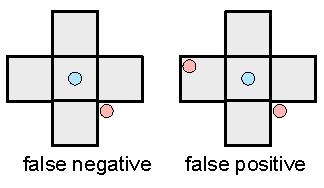
\includegraphics[width=0.4\textwidth]{resources/basic-point-cloud/grid-bad-cases.pdf}
	\caption{Schematic illustration of false positive/negative issues in grid-based nearest neighbor search}
	\label{fig:grid-bad-cases}
\end{figure}

This naturally leads to the question: Could we abandon fixed-distance partitioning in favor of more intelligent spatial subdivision methods? This is precisely the rationale behind K-d trees. However, compared to the tree-based data structures we'll discuss later, grid and voxel methods achieve respectable performance using simpler data structures while being inherently parallelizable. Together with tree structures, voxel-based approaches form the foundation of most modern matching algorithms and SLAM systems \cite{Koide2019,Koide2020,Huang2021a,Bai2022}. 

The key trade-off emerges: While tree structures provide more adaptive spatial partitioning that better handles boundary cases, their increased algorithmic complexity often offsets their theoretical advantages in practical implementations where parallel processing and memory locality significantly impact real-world performance. This explains why many state-of-the-art systems employ hybrid approaches, combining the brute-force efficiency of voxel methods with the adaptive precision of tree structures where needed.

Notably, the precision/recall metrics shown in our earlier benchmarks (0.91 precision for 3D voxels vs 0.73 for 2D 8-neighbor grids) demonstrate that dimensionality plays a crucial role - the additional spatial information in 3D inherently provides better disambiguation between true and false neighbors, even using similar search methodologies. This dimensional advantage becomes particularly important in applications like autonomous driving where the vertical dimension often provides critical discriminative information.

\subsection{Binary Trees and K-d Trees}
\label{sec:binary-tree}
Let us now return to the earlier idea: searching in a sorted container can significantly save time. Following this line of thought, we can propose data structures similar to binary search, such as Binary Search Trees (BST) and their high-dimensional counterpart: K-dimensional trees (K-d trees). Since point clouds belong to three-dimensional space, we will focus on introducing K-d trees.  

From data structure knowledge, searching in a sorted container using binary search is more efficient than linear search: binary search has a complexity of \(O(\log_2 N)\), while linear search is \(O(N)\). The binary search process itself is tree-like: for a given element \(x\) and container \(V\), we first compare \(x\) with the central element of the container. If \(x\) is smaller, we continue comparing it with the left half of the container; otherwise, we compare it with the right half. Based on this relationship, we can reorganize the container using a tree data structure to facilitate faster searches.  

This process does not require predefined partitioning thresholds. Additionally, binary trees have a space complexity of \(O(N)\) and a time complexity of \(O(\log_2 N)\), making them an ideal search method. The only drawback is that this approach is only effective for one-dimensional data. For high-dimensional data, points may be well-separated in one dimension but overlap in another, making binary trees and binary search unsuitable for direct application.  

The K-d tree \cite{Bentley1975}, originally proposed by Bentley Jon Louis, is a high-dimensional extension of binary trees, as illustrated in Figure~\ref{fig:kdtree}. A K-d tree is also a type of binary tree, where each node consists of left and right branches. In binary trees, we can use a single dimension to distinguish between left and right branches. However, in K-d trees, since we need to partition high-dimensional data, we use \textbf{hyperplanes} to separate the left and right branches (though for 3D points, the hyperplane is simply an ordinary 2D plane).  

There are methodological differences in \textbf{how to partition} the data. Theoretically, finding a hyperplane to separate two high-dimensional point sets can be viewed as a support vector machine (SVM) classification problem \cite{Cortes1995}. However, for K-d trees in SLAM, where both construction and search processes need to run in real-time, we typically choose simpler partitioning methods. The simplest is the \textbf{axis-aligned splitting plane}. Despite its intimidating name, it simply involves splitting the point cloud along any one of the axes, making it very easy to implement.  

\begin{figure}[!htp]
	\centering
	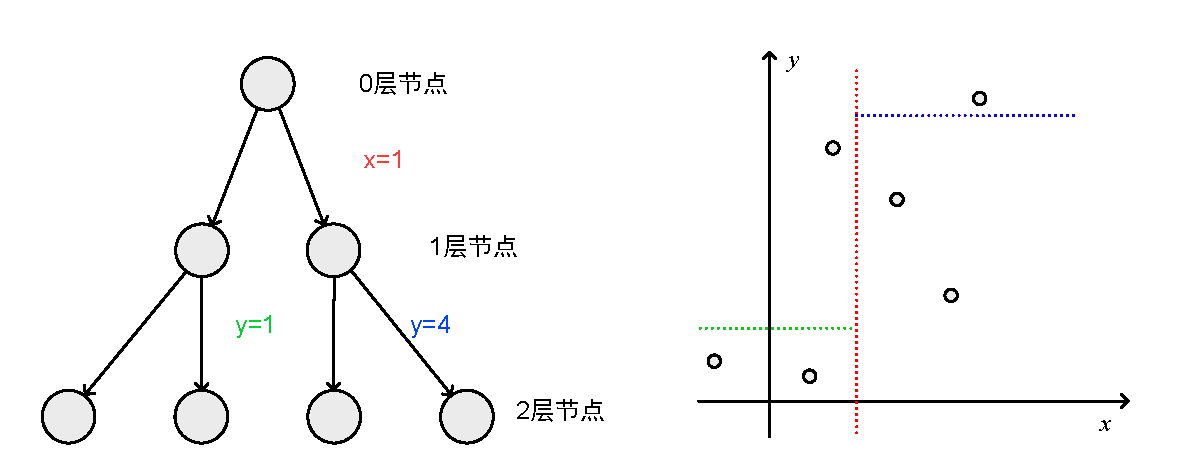
\includegraphics[width=0.8\textwidth]{resources/basic-point-cloud/kdtree.pdf}
	\caption{Schematic of a K-d tree. The left side shows the tree structure in the program, while the right side illustrates the partitioning relationships of each node.}
	\label{fig:kdtree}
\end{figure}

We can construct a K-d tree for a point cloud of any dimensionality, referred to as the \textbf{building process} or \textbf{tree construction}. Subsequently, we can perform kNN searches for any point in space, referred to as the \textbf{search process}. Depending on the search method, K-d trees can be categorized into \textbf{range search} (Search by range) and \textbf{K-nearest neighbor search} (Search by K nearest neighbors), with minor differences in their implementations.  

In a K-d tree, we use a tree structure to represent the spatial relationships of the point cloud, with the following rules:  
1. Each node has left and right branches.  
2. Leaf nodes represent points in the original point cloud. In practice, we can store point indices instead of the points themselves to save space.  
3. Non-leaf nodes store a splitting axis and a splitting threshold to define how the left and right branches are partitioned. For example, \(x = 1\) can be stored as splitting along the first axis with a threshold of 1. We define the left branch as taking values less than the threshold and the right branch as taking values greater than the threshold.  

With these conventions, we can implement the construction and search algorithms for K-d trees. Below, we briefly describe the algorithmic steps and then provide implementations and discussions of the results. Since K-d trees are fundamentally tree structures, most algorithms can be concisely implemented using recursion.

\subsection{Construction of K-d Trees}
In the construction process of a K-d tree, we primarily consider how to partition a given point cloud. Different partitioning strategies exist depending on the method used. Traditional approaches either alternate coordinate axes in a fixed order \cite{DeBerg1997} or calculate the dispersion of the current point cloud along each axis and select the axis with the highest dispersion as the splitting axis. Here, we focus on the latter method. Additionally, there are various variants such as implicit K-d trees \cite{Gros2007}, min-max K-d trees \cite{Duvenhage2009}, and relaxed K-d trees \cite{Duch1998}, which employ different strategies to handle partitioning or leaf node storage. For now, we will focus on the basic K-d tree.

\begin{mdframed}
	\textbf{Construction of a K-d Tree:}
	\begin{enumerate}
		\item \textbf{Input:} Point cloud data \(\mathbf{X} = \{\mathbf{x}_1, \ldots, \mathbf{x}_n\}\), where \(\mathbf{x}_i \in \mathbb{R}^{k}\).
		\item Consider inserting subset \(\mathbf{X}_n \subset \mathbf{X}\) into node \(n\):
		\item If \(\mathbf{X}_n\) is empty, exit.
		\item If \(\mathbf{X}_n\) contains only one point, mark it as a leaf node and exit.
		\item Calculate the variance of \(\mathbf{X}_n\) along each axis and select the axis \(j\) with the highest dispersion. Use the mean \(m_j = \mathbf{X}_n[j]\) as the splitting threshold.
		\item For each \(\mathbf{x} \in \mathbf{X}_n\), if \(\mathbf{x}[j] < m_j\), insert it into the left child node; otherwise, insert it into the right child node.
		\item Recursively apply the above steps until all points are inserted into the tree.
	\end{enumerate}
\end{mdframed}

The above algorithm can be easily implemented recursively.

\subsection{Searching in K-d Trees}
Searching in a K-d tree essentially involves traversing a binary tree. Similar to binary trees, traversal methods such as pre-order, in-order, and post-order can be applied. The unique feature of K-d trees is that we can prune unnecessary branches to improve search efficiency.

Figure~\ref{fig:kdtree-split-plane} illustrates the process of searching for a query point in a K-d tree. Note that although the query point (blue) falls on the left side of the K-d tree, its nearest neighbor may not necessarily be on the left. The position of the splitting plane is determined by the point cloud distribution during tree construction. During the search, the nearest neighbor can be on either side. However, due to the splitting plane, points on the right side have a minimum distance \(d\) to the query point, which is the perpendicular distance from the query point to the splitting plane. If a point on the left side is found with a distance smaller than \(d\), the right branch can be pruned. Conversely, if the nearest neighbor on the left is farther than \(d\), the right branch must be searched. This is the fundamental principle of K-d tree traversal.

\begin{figure}[!htp]
	\centering
	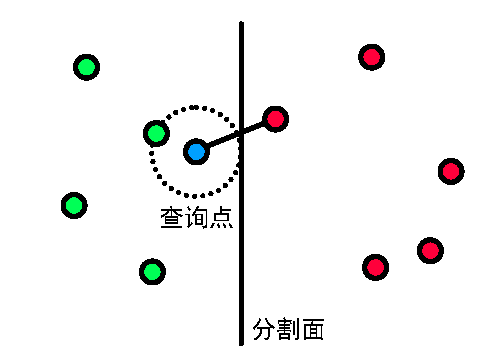
\includegraphics[width=0.4\textwidth]{resources/basic-point-cloud/kdtree-split-plane.pdf}
	\caption{Schematic of K-d tree pruning. In this figure, the distance from the splitting plane of the right branch exceeds the current nearest neighbor distance, indicating that points on the right must be farther than the current best solution. Thus, the right branch can be skipped.}
	\label{fig:kdtree-split-plane}
\end{figure}

Based on this principle, the nearest neighbor search in a K-d tree can be described as follows:

\begin{mdframed}
	\textbf{Nearest Neighbor Search in K-d Trees:}
	\begin{enumerate}
		\item \textbf{Input:} K-d tree \(T\), query point \(\mathbf{x}\).
		\item \textbf{Output:} Nearest neighbor of \(\mathbf{x}\).
		\item Let the current node be \(n_c\), initially the root node. Let \(d\) be the current minimum distance.
		\begin{enumerate}
			\item If \(n_c\) is a leaf, compute the distance between \(n_c\) and \(\mathbf{x}\). If it is smaller than \(d\), update \(n_c\) as the nearest neighbor and backtrack to its parent.
			\item If \(n_c\) is not a leaf, determine which side of \(n_c\) \(\mathbf{x}\) lies on. If the side containing \(\mathbf{x}\) has not been explored, prioritize exploring that side.
			\item Determine whether to explore the other side of \(n_c\). Compute the distance \(d'\) from \(\mathbf{x}\) to the splitting plane of \(n_c\). If \(d' < d\), the other side must be explored; otherwise, skip it.
			\item If both sides have been explored or need not be explored, backtrack to the parent node until \(n_c\) becomes the root node.
		\end{enumerate}
	\end{enumerate}
\end{mdframed}

For the \(k\)-nearest neighbor problem, the nearest neighbor becomes a set of points, and the distance threshold \(d\) is updated dynamically:

\begin{mdframed}
	\textbf{\(k\)-Nearest Neighbor Search in K-d Trees:}
	\begin{enumerate}
		\item \textbf{Input:} K-d tree \(T\), query point \(\mathbf{x}\), number of neighbors \(k\).
		\item \textbf{Output:} Set of \(k\)-nearest neighbors \(N\).
		\item Let the current node be \(n_c\), initially the root node. Define \(S(n_c)\) as the \(k\)-nearest neighbor search under \(n_c\):
		\begin{enumerate}
			\item If \(n_c\) is a leaf, compute its distance to \(\mathbf{x}\). If it is smaller than the largest distance in \(N\), add \(n_c\) to \(N\). If \(|N| > k\), remove the farthest point in \(N\).
			\item Determine which side of \(n_c\) \(\mathbf{x}\) lies on and recursively call \(S(n_c.\text{left})\) or \(S(n_c.\text{right})\).
			\item Determine whether to explore the other side of \(n_c\). The exploration condition is: if \(|N| < k\), explore; if \(|N| = k\) and the distance from \(\mathbf{x}\) to the splitting plane is less than the largest distance in \(N\), explore.
			\item If the other side need not be explored, return; otherwise, continue the search on the other side.
		\end{enumerate}
	\end{enumerate}
\end{mdframed}

In the worst case, this process may traverse the entire tree. If the query point lies near multiple splitting planes and the other side contains closer points, the K-d tree degenerates to linear search (brute-force), and its performance may even be worse due to the overhead of node traversal. The time complexity for searching a single nearest neighbor is logarithmic \(O(\log_2 N)\), while searching for \(k\) neighbors depends on the distribution of the point cloud. If the point cloud is well-distributed and the initial \(k\) neighbors are close, pruning can significantly reduce the search space. However, for large \(k\) or poorly distributed point clouds, more branches may need to be traversed.

In practice, it is often unnecessary to strictly find the exact \(k\)-nearest neighbors (e.g., if the \(k\)-th neighbor is much farther away). Thus, optimizations can be applied, such as setting a maximum number of points to visit or a timeout to terminate the search early. Another common optimization is to introduce a ratio \(\alpha\) for the pruning condition. Let \(d_{\text{max}}\) be the maximum distance in the current \(k\)-nearest neighbors and \(d_{\text{split}}\) be the distance to the splitting plane. If \(d_{\text{split}} > \alpha d_{\text{max}}\), the branch is pruned. Choosing \(\alpha \leq 1\) allows for more aggressive pruning.

\subsubsection{Implementation of K-d Tree Construction}
Below, we will briefly implement a K-d tree. While there are many open-source implementations of K-d trees, the teaching process often uses simpler and more understandable versions. We will first implement our own K-d tree and then compare it with the K-d tree in PCL, as well as with the algorithms mentioned earlier.

First, let's define the basic structure of the K-d tree. Each node contains pointers to its left and right children, as well as information about the splitting plane:

\begin{lstlisting}[language=c++, caption=src/ch5/kdtree.cc]
struct KdTreeNode {
	int id_ = -1;
	int point_idx_ = 0;            // Point index
	int axis_index_ = 0;           // Splitting axis
	float split_thresh_ = 0.0;     // Splitting threshold
	KdTreeNode* left_ = nullptr;   // Left subtree
	KdTreeNode* right_ = nullptr;  // Right subtree
	KdTreeNode* up_ = nullptr;     // Parent node
	
	bool IsLeaf() const { return left_ == nullptr && right_ == nullptr; }  // Whether it is a leaf
};
\end{lstlisting}

Each node stores the splitting axis and threshold. For example, if the splitting axis is the first axis (e.g., x-axis) and the threshold is 0.5, points with \(x < 0.5\) will be placed in the left subtree, while points with \(x \geq 0.5\) will be placed in the right subtree. Additionally, we record the ID of each node to facilitate indexing the tree without writing recursive code. Below are the basic member variables of the K-d tree:

\begin{lstlisting}[language=c++,caption=src/ch5/kdtree.h]
class KdTree {
	private:
	int k_ = 5;                                   // Number of nearest neighbors for KNN
	std::shared_ptr<KdTreeNode> root_ = nullptr;  // Root node
	std::vector<Vec3f> cloud_;                    // Input point cloud
	std::map<int, KdTreeNode*> nodes_;            // For bookkeeping
	size_t size_ = 0;                             // Number of leaf nodes
	int tree_node_id_ = 0;                        // Assigns IDs to K-d tree nodes
};
\end{lstlisting}

The K-d tree class holds a pointer to the root node, allowing traversal of the entire tree. We also maintain a map of node IDs to node pointers. Next, let's implement the tree construction process. Building the tree requires an input point cloud. We record the point cloud indices in the leaf nodes:

\begin{lstlisting}[language=c++,caption=src/ch5/kdtree.cc]
bool KdTree::BuildTree(const CloudPtr &cloud) {
	// Input validation code omitted
	IndexVec idx(cloud->size());
	for (int i = 0; i < cloud->points.size(); ++i) {
		idx[i] = i;
	}
	
	Insert(idx, root_.get());
	
	return true;
}

void KdTree::Insert(const IndexVec &points, KdTreeNode *node) {
	nodes_.insert({node->id_, node});
	
	if (points.empty()) {
		return;
	}
	
	if (points.size() == 1) {
		// Leaf node
		size_++;
		node->point_idx_ = points[0];
		return;
	}
	
	IndexVec left, right;
	FindSplitAxisAndThresh(points, node->axis_index_, node->split_thresh_, left, right);
	
	const auto create_if_not_empty = [&node, this](KdTreeNode *&new_node, const IndexVec &index) {
		if (!index.empty()) {
			new_node = new KdTreeNode;
			new_node->up_ = node;
			new_node->id_ = tree_node_id_++;
			
			Insert(index, new_node);
		}
	};
	
	create_if_not_empty(node->left_, left);
	create_if_not_empty(node->right_, right);
}

bool KdTree::FindSplitAxisAndThresh(const IndexVec &point_idx, int &axis, float &th, IndexVec &left, IndexVec &right) {
	// Calculate variance along each axis using functions from math_utils.h
	Vec3f var;
	Vec3f mean;
	math::ComputeMeanAndCovDiag(point_idx, mean, var, [this](const int &idx) { return cloud_[idx]; });
	int max_i, max_j;
	var.maxCoeff(&max_i, &max_j);
	axis = max_i;
	th = mean[axis];
	
	if (var.squaredNorm() < 1e-7) {
		// Edge case: All points have the same value. Split into left and right halves arbitrarily.
		// Rare in real data but possible in synthetic data.
		for (int i = 0; i < point_idx.size(); ++i) {
			if (i < point_idx.size() / 2) {
				left.emplace_back(point_idx[i]);
			} else {
				right.emplace_back(point_idx[i]);
			}
		}
		return true;
	}
	
	for (const auto &idx : point_idx) {
		if (cloud_[idx][axis] < th) {
			left.emplace_back(idx);
		} else {
			right.emplace_back(idx);
		}
	}
	
	if (point_idx.size() > 1) {
		// For non-trivial splits, ensure both subtrees are non-empty
		assert(left.empty() == false && right.empty() == false);
	}
	
	return true;
}
\end{lstlisting}

Here's the translation preserving all LaTeX commands exactly as in the original:

\subsection{Implementation of K-d Tree Construction}
The tree construction process is straightforward, implemented through recursive calls to the \texttt{Insert} function. If the input parameter \texttt{points} contains only one point, the current \texttt{node} becomes a leaf, and the point index is directly assigned. Otherwise, we calculate the variance along each axis, select the axis with the highest variance as the splitting axis, and use the mean value as the threshold. To handle edge cases where all points share identical coordinates (resulting in zero variance), we include a variance check.

Below is a test case for the tree construction process. We define four points on the \( z = 0 \) plane and observe the resulting tree structure:

\begin{lstlisting}[language=c++,caption=src/ch5/test\_nn.cc]
TEST(CH5_TEST, KDTREE_BASICS) {
	sad::CloudPtr cloud(new sad::PointCloudType);
	sad::PointType p1, p2, p3, p4;
	p1.x = 0; p1.y = 0; p1.z = 0;
	p2.x = 1; p2.y = 0; p2.z = 0;
	p3.x = 0; p3.y = 1; p3.z = 0;
	p4.x = 1; p4.y = 1; p4.z = 0;
	
	cloud->points.push_back(p1);
	cloud->points.push_back(p2);
	cloud->points.push_back(p3);
	cloud->points.push_back(p4);
	
	sad::KdTree kdtree;
	kdtree.BuildTree(cloud);
	kdtree.PrintAll();
	
	SUCCEED();
}
\end{lstlisting}

Compile and run the program:
\begin{lstlisting}[caption=Terminal input:]
bin/test_nn --gtest_filter=CH5_TEST.KDTREE_BASICS    
Note: Google Test filter = CH5_TEST.KDTREE_BASICS
[==========] Running 1 test from 1 test suite.
[----------] Global test environment set-up.
[----------] 1 test from CH5_TEST
[ RUN      ] CH5_TEST.KDTREE_BASICS
I0118 10:25:14.149652 295100 kdtree.cc:241] node: 0, axis: 0, th: 0.5
I0118 10:25:14.149777 295100 kdtree.cc:241] node: 1, axis: 1, th: 0.5
I0118 10:25:14.149780 295100 kdtree.cc:239] leaf node: 2, idx: 0
I0118 10:25:14.149780 295100 kdtree.cc:239] leaf node: 3, idx: 2
I0118 10:25:14.149781 295100 kdtree.cc:241] node: 4, axis: 1, th: 0.5
I0118 10:25:14.149782 295100 kdtree.cc:239] leaf node: 5, idx: 1
I0118 10:25:14.149783 295100 kdtree.cc:239] leaf node: 6, idx: 3
[       OK ] CH5_TEST.KDTREE_BASICS (0 ms)
\end{lstlisting}

\begin{figure}[!htp]
	\centering
	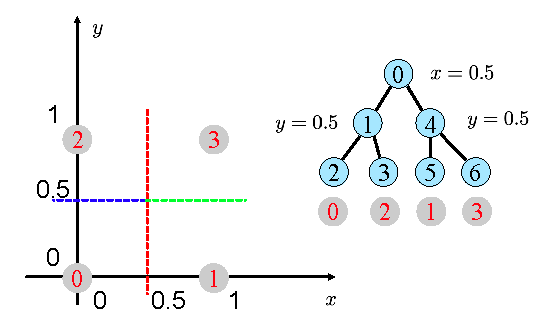
\includegraphics[width=0.8\textwidth]{resources/basic-point-cloud/kdtree-example.pdf}
	\caption{Schematic of the K-d tree construction for this example. Gray circles show point cloud IDs, while blue circles indicate K-d tree node IDs.}
	\label{fig:kdtree-example}
\end{figure}

The experimental results are illustrated in Figure~\ref{fig:kdtree-example}, displaying the splitting thresholds and leaf node information of the K-d tree. The constructed tree for these four points has two levels, with each splitting plane positioned at the midpoint between two points. Notably, since each split divides the remaining point cloud into two equal subsets, this K-d tree remains balanced, avoiding significant imbalance between left and right subtrees.  

Key observations:
1. \textbf{Axis Selection}: The first split occurs along the x-axis (axis 0) at \( x = 0.5 \), separating points \( p1, p3 \) (left) from \( p2, p4 \) (right).  
2. \textbf{Recursive Splitting}: Each subset is further split along the y-axis (axis 1) at \( y = 0.5 \), resulting in four leaf nodes.  
3. \textbf{Balance}: The tree depth is minimized due to equal partitioning, ensuring optimal search performance.  

This example demonstrates how K-d trees adaptively partition space based on data distribution, a property critical for efficient nearest neighbor searches in higher-dimensional datasets. The balance achieved here is a direct consequence of uniform point spacing, though real-world data may require additional balancing techniques (e.g., median-based splits) to maintain efficiency.

\subsubsection{Implementing K-Nearest Neighbors in K-d Trees}
Now let's implement the K-nearest neighbors (KNN) algorithm for K-d trees. When \(K=1\), this naturally becomes the nearest neighbor algorithm, so we don't need to implement a separate nearest neighbor search. First, we define a structure to record nodes and distances, along with its sorting method:

\begin{lstlisting}[language=c++,caption=src/ch5/kdtree.h]
/// For recording KNN results
struct NodeAndDistance {
	NodeAndDistance(KdTreeNode* node, float dis2) : node_(node), distance2_(dis2) {}
	KdTreeNode* node_ = nullptr;
	float distance2_ = 0;  // Squared distance for comparison
	
	bool operator<(const NodeAndDistance& other) const { return distance2_ < other.distance2_; }
};
\end{lstlisting}

We then use a priority queue to manage the KNN results. This queue maintains order during insertion, making it suitable for storing nearest neighbor results. The K-d tree nearest neighbor search is implemented as follows:

\begin{lstlisting}[language=c++,caption=src/ch5/kdtree.cc]
/// Compute K nearest neighbors
bool KdTree::GetClosestPoint(const PointType &pt, std::vector<int> &closest_idx, int k) {
	if (k > size_) {
		LOG(ERROR) << "cannot set k larger than cloud size: " << k << ", " << size_;
		return false;
	}
	k_ = k;
	
	std::priority_queue<NodeAndDistance> knn_result;
	Knn(ToVec3f(pt), root_.get(), knn_result);
	
	// Sort and return results
	closest_idx.resize(knn_result.size());
	for (int i = closest_idx.size() - 1; i >= 0; --i) {
		// Insert in reverse order
		closest_idx[i] = knn_result.top().node_->point_idx_;
		knn_result.pop();
	}
	return true;
}

/// Search for nearest neighbors of pt under node and add to result queue
void KdTree::Knn(const Vec3f &pt, KdTreeNode *node, std::priority_queue<NodeAndDistance> &knn_result) const {
	if (node->IsLeaf()) {
		// If leaf, check if it can be inserted
		ComputeDisForLeaf(pt, node, knn_result);
		return;
	}
	
	// Determine which side pt falls on and prioritize searching that subtree
	// Then check if the other subtree needs to be searched
	KdTreeNode *this_side, *that_side;
	if (pt[node->axis_index_] < node->split_thresh_) {
		this_side = node->left_;
		that_side = node->right_;
	} else {
		this_side = node->right_;
		that_side = node->left_;
	}
	
	Knn(pt, this_side, knn_result);
	if (NeedExpand(pt, node, knn_result)) {  // Note: comparison is with current best
		Knn(pt, that_side, knn_result);
	}
}

void KdTree::ComputeDisForLeaf(const Vec3f &pt, KdTreeNode *node,
std::priority_queue<NodeAndDistance> &knn_result) const {
	// Compare with current results and insert if better than worst distance
	float dis2 = Dis2(pt, cloud_[node->point_idx_]);
	if (knn_result.size() < k_) {
		// Not enough results yet
		knn_result.push({node, dis2});
	} else {
		// Already have k results, compare with current worst
		if (dis2 < knn_result.top().distance2_) {
			knn_result.push({node, dis2});
			knn_result.pop();
		}
	}
}

bool KdTree::NeedExpand(const Vec3f &pt, KdTreeNode *node, std::priority_queue<NodeAndDistance> &knn_result) const {
	if (knn_result.size() < k_) {
		return true;
	}
	
	// Check splitting plane distance to see if better results might exist
	float d = pt[node->axis_index_] - node->split_thresh_;
	if ((d * d) < knn_result.top().distance2_) {
		return true;
	} else {
		return false;
	}
}
\end{lstlisting}

The nearest neighbor function recursively calls the Knn function to perform the search. For leaf nodes, it compares the node's distance with the worst distance in the current KNN results. If better, it inserts into the priority queue. The NeedExpand function determines whether to search the other subtree based on the splitting plane distance.

Let's test our K-d tree implementation. We compare against brute-force results for ground truth and benchmark against PCL's K-d tree:

\begin{lstlisting}[language=sh, caption=Terminal input:]
bin/test_nn --gtest_filter=CH5_TEST.KDTREE_KNN 
I0118 17:07:02.307432 318029 sys_utils.h:32] Method Kd Tree build avg time/calls: 4.34059/1 ms.
I0118 17:07:02.307545 318029 test_nn.cc:234] Kd tree leaves: 18869, points: 18869
I0118 17:07:03.029914 318029 sys_utils.h:32] Method Kd Tree 5NN multi-thread avg time/calls: 3.01146/1 ms.
I0118 17:07:03.030046 318029 test_nn.cc:65] truth: 93895, esti: 93895
I0118 17:07:04.396924 318029 test_nn.cc:93] precision: 1, recall: 1, fp: 0, fn: 0
I0118 17:07:04.396939 318029 test_nn.cc:246] building kdtree pcl
I0118 17:07:04.398665 318029 sys_utils.h:32] Method Kd Tree build avg time/calls: 1.68209/1 ms.
I0118 17:07:04.398671 318029 test_nn.cc:252] searching pcl
I0118 17:07:04.411710 318029 sys_utils.h:32] Method Kd Tree 5NN in PCL avg time/calls: 12.9858/1 ms.
I0118 17:07:04.411908 318029 test_nn.cc:65] truth: 93895, esti: 93895
I0118 17:07:05.779804 318029 test_nn.cc:93] precision: 1, recall: 1, fp: 0, fn: 0
I0118 17:07:05.779814 318029 test_nn.cc:274] done.
\end{lstlisting}

The K-d tree achieves perfect precision and recall (100\%). Compared to PCL's implementation, our K-d tree takes longer to build (likely due to maintaining an additional node list) but demonstrates faster concurrent nearest neighbor searches.

\subsubsection{Implementing K-d Tree Construction and Nearest Neighbor Search}  

Through code implementation, we observe that the most critical part of the K-d tree nearest neighbor algorithm is **pruning**, and the pruning condition is that no closer nearest neighbor exists on the other side of the tree structure. Let the current farthest nearest neighbor distance be $d_{max}$, and the splitting plane distance be $d_{split}$. The pruning criterion can then be expressed as:  
\begin{equation}\label{key}  
	d_{split} > d_{max}.  
\end{equation}  

However, in the worst-case scenario, if the current nearest neighbor found is poor, we might need to search distant branches for a potentially closer neighbor. This is a situation we wish to avoid. Therefore, we can slightly modify the above criterion by introducing a scaling factor $\alpha$:  
\begin{equation}\label{key}  
	d_{split} > \alpha d_{max}.  
\end{equation}  

When $\alpha < 1$, the pruning condition is relaxed, making the K-nearest neighbor search faster, but we no longer guarantee finding the **exact nearest neighbor** (since their branches may have been pruned). This approach is referred to as **Approximate Nearest Neighbor (ANN)**. The ANN problem is more flexible than the KNN problem, allowing for various algorithmic and data structure approximations. In our code, we implement it as follows:  

\begin{lstlisting}[language=c++,caption=src/ch5/kdtree.cc]  
bool KdTree::NeedExpand(const Vec3f &pt, KdTreeNode *node, std::priority_queue<NodeAndDistance> &knn_result) const {  
	if (knn_result.size() < k_) {  
		return true;  
	}  
	
	if (approximate_) {  
		float d = pt[node->axis_index_] - node->split_thresh_;  
		if ((d * d) < knn_result.top().distance2_ * alpha_) {  
			return true;  
		} else {  
			return false;  
		}  
	} else {  
		// Check the splitting plane distance to see if a closer neighbor exists  
		float d = pt[node->axis_index_] - node->split_thresh_;  
		if ((d * d) < knn_result.top().distance2_) {  
			return true;  
		} else {  
			return false;  
		}  
	}  
}  
\end{lstlisting}  

The performance of the K-d tree with approximate nearest neighbor enabled (with $\alpha=0.1$) is as follows:  
\begin{lstlisting}[caption=Terminal output:]  
I0118 17:31:41.829752 320541 sys_utils.h:32] Method Kd Tree build average call time/count: 4.34565/1 ms.  
I0118 17:31:41.829856 320541 test_nn.cc:227] Kd tree leaves: 18869, points: 18869  
I0118 17:31:42.553129 320541 sys_utils.h:32] Method Kd Tree 5NN multithreaded average call time/count: 2.10658/1 ms.  
I0118 17:31:42.553233 320541 test_nn.cc:65] truth: 93895, esti: 93895  
I0118 17:31:44.371816 320541 test_nn.cc:91] precision: 0.771319, recall: 0.771319, fp: 21472, fn: 21472  
I0118 17:31:44.371834 320541 test_nn.cc:239] building kdtree pcl  
I0118 17:31:44.373656 320541 sys_utils.h:32] Method Kd Tree build average call time/count: 1.80198/1 ms.  
I0118 17:31:44.373662 320541 test_nn.cc:244] searching pcl  
I0118 17:31:44.387229 320541 sys_utils.h:32] Method Kd Tree 5NN in PCL average call time/count: 13.5384/1 ms.  
I0118 17:31:44.387405 320541 test_nn.cc:65] truth: 93895, esti: 93895  
I0118 17:31:45.723769 320541 test_nn.cc:91] precision: 1, recall: 1, fp: 0, fn: 0  
I0118 17:31:45.723780 320541 test_nn.cc:266] done.  
\end{lstlisting}  

It can be seen that the approximate method leads to some decline in precision and recall, with both metrics dropping to around 0.77, but there is an improvement in search speed. Compared to the algorithms in the previous section, the K-d tree is significantly better than brute-force search but slower than 2D and 3D voxel-based methods. If construction time is considered, it is even slower. In terms of performance, the K-d tree allows tuning the $\alpha$ parameter, enabling a balance between speed and accuracy. In contrast, grid-based methods, while very fast, often struggle to achieve satisfactory recall rates.  

The K-d tree in this chapter is implemented recursively, making the code concise, but it may encounter stack overflow issues with extremely large point clouds. Readers can modify it to an iterative implementation. Additionally, there are many improved versions of the K-d tree, which we will not implement here. Interested readers can explore open-source K-d tree algorithms such as \cite{Cai2021} for comparison. Furthermore, to save space, we have omitted discussions on other topics, such as how to delete a point from a K-d tree, how to balance a K-d tree, etc. Readers interested in these aspects are encouraged to refer to relevant literature.

\subsection{Quadtree and Octree}  

The K-d tree methods introduced earlier use a binary tree as the basic data structure. However, can we have more branches beyond just binary trees? The answer is yes. In two-dimensional and three-dimensional spaces, we have two corresponding approaches: the **Quadtree** \cite{Samet1984} and the **Octree** \cite{Meagher1982, Shaffer1987}. If we do not partition space using grids, other tree-based methods can also be derived. Since these two approaches follow the same underlying principle—only differing in spatial dimensionality—we will discuss them together.  

In a quadtree, each node has four children, while in an octree, each node has eight. This naturally corresponds to physical space: a rectangle can be divided into four equal parts by its center, and a 3D cube can be split into eight equal parts. The parent node represents the larger rectangle/cube, and the child nodes represent the subdivided rectangles/cubes, forming the quadtree and octree structures. This structure inherently defines the rules for space partitioning. Therefore, similar to the K-d tree, we can construct a quadtree/octree model for a 2D/3D point cloud and use analogous methods to perform nearest neighbor searches. Due to their more uniform spatial partitioning, quadtrees and octrees can also be used to describe data covering an entire space, such as maps.  

\begin{figure}[!htp]  
	\centering  
	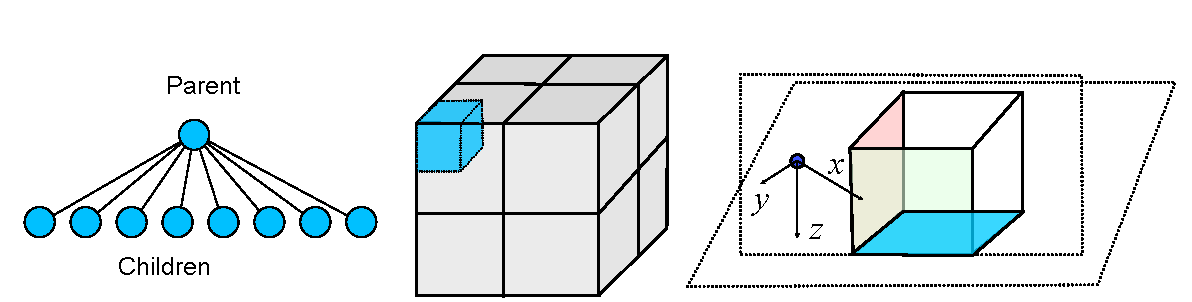
\includegraphics[width=1.0\textwidth]{resources/basic-point-cloud/octo-tree.pdf}  
	\caption{Schematic diagram of octree principles and distance computation. Left: The data structure of an octree; Middle: The partitioning method of an octree; Right: The distance calculation from an external point to a cube.}  
	\label{fig:octo-tree}  
\end{figure}

\subsubsection{Octree Construction}
Our focus is on 3D point cloud problems, so here we implement an octree algorithm, which also serves as a performance comparison experiment for readers. To maintain consistency, we try to mimic the K-d tree interface when implementing the octree, which also demonstrates their similarity. The main differences between octrees and K-d trees are:

\begin{enumerate}
	\item K-d trees use splitting planes to distinguish point sets, while octrees use cubic forms. For this purpose, we implemented a \texttt{Box3D} structure to handle the relationship between points and the octree.
	\item When building a K-d tree, the splitting planes are dynamically determined; in octrees, the subdivision of cubes is fixed (dividing into eight parts from the center). This means an octree node can always be expanded, but its child nodes may contain no point cloud. In this implementation, we retain those leaf nodes without corresponding point clouds. Of course, readers can choose to delete these leaf nodes, which would reduce the total number of nodes in the tree.
	\item During initial octree construction, we compute the bounding box of the entire point cloud as the root node's boundary box. This bounding box doesn't need to be a perfect cube. We allow it to be longer in certain dimensions, as long as subsequent subdivisions still follow the \textbf{eight-way split} rule. Readers can also enforce a perfect cube bounding box, but this may make the tree deeper and reduce search efficiency.
	\item The nearest neighbor search process in octrees is similar to K-d trees and also involves pruning. We use the \textbf{maximum perpendicular distance from the query point to the outer boundary of the bounding box} as the pruning criterion (see Figure~\ref{fig:octo-tree} for illustration). In this schematic, the query point is outside the grid in the x-direction but inside in the y and z directions. Therefore, the lower bound for the distance between the query point and the point cloud inside the cube should be the distance in the x-direction. If two or three axes are outside the cube, the longest axis should be taken as the distance lower bound. Readers can visualize this themselves. Of course, this lower bound could be estimated more precisely (e.g., by calculating the distance between the query point and the eight vertices of the cube), but we should ensure the distance calculation method is as simple as possible while maintaining effective pruning.
\end{enumerate}

With these differences in mind, we describe the octree construction and search algorithms:

\begin{mdframed}
	\textbf{Octree Construction:}
	\begin{enumerate}
		\item Input: Point cloud data $\mathbf{X} = \{\mathbf{x}_1, \ldots, \mathbf{x}_n\}$, where $\mathbf{x}_i \in \mathbb{R}^{k}$.
		\item Consider inserting subset $\mathbf{X}_n \subseteq \mathbf{X}$ into node $n$:
		\item If $\mathbf{X}_n$ is empty, exit;
		\item If $\mathbf{X}_n$ contains only one point, mark it as a leaf node and exit;
		\item Expand $n$ following the \textbf{eight-way split} rule.
		\item For each $\mathbf{x} \in \mathbf{X}_n$, record which child node contains $\mathbf{x}$. Then recursively apply the construction method to the child node and its corresponding point cloud.
		\item Repeat the above steps until all points are inserted into the tree.
	\end{enumerate}
\end{mdframed}

\subsubsection{Octree Search}
The k-nearest neighbor search algorithm for octrees can also be obtained by slightly modifying the K-d tree approach:

\begin{mdframed}
	\textbf{Octree k-Nearest Neighbor Search:}
	\begin{enumerate}
		\item Input: Octree $T$, query point $\mathbf{x}$, number of neighbors $k$;
		\item Output: k-nearest neighbor set $N$;
		\item Let the current node be $n_c$ (initially the root node). Define function $S(n_c)$ as performing k-nearest neighbor search under $n_c$:
		\begin{enumerate}
			\item If $n_c$ is a leaf, calculate whether the distance between $n_c$ and $\mathbf{x}$ is smaller than the maximum distance in $N$; if so, add $n_c$ to $N$. If $|N| > k$, remove the farthest matching point from $N$;
			\item Determine which child node of $n_c$ contains $\mathbf{x}$. If $\mathbf{x}$ is outside $n_c$'s bounding box, expand all child nodes; if inside, prioritize expanding the child node containing $\mathbf{x}$.
			\item Determine whether to expand other child nodes of $n_c$. The expansion condition: if $|N|<k$, expansion is mandatory; if $|N|=k$ and the previously calculated distance between $\mathbf{x}$ and $n_c$ is less than the maximum matching distance in $N$, also expand;
			\item If $n_c$'s child nodes don't need expansion, return; otherwise, continue calling the neighbor search algorithm for other nodes.
		\end{enumerate}
	\end{enumerate}
\end{mdframed}

\subsubsection{Code Implementation}  
Now let's implement the octree described earlier. An octree node consists of its bounding box and eight child nodes, defined as follows:

\begin{lstlisting}[language=c++,caption=src/ch5/octo\_tree.h]
struct Box3D {
	Box3D() = default;
	Box3D(float min_x, float max_x, float min_y, float max_y, float min_z, float max_z)
	: min_{min_x, min_y, min_z}, max_{max_x, max_y, max_z} {}
	
	float min_[3] = {0};
	float max_[3] = {0};
};

/// Octree node
struct OctoTreeNode {
	int id_ = -1;
	int point_idx_ = -1;                    // Point index, -1 means invalid
	bool box_set_ = false;                  // Whether bounding box is set
	Box3D box_;                             // Bounding box
	OctoTreeNode* children[8] = {nullptr};  // Child nodes
	OctoTreeNode* parent_ = nullptr;        // Parent node
};
\end{lstlisting}

Each bounding box consists of minimum and maximum values along three axes. The actual code also implements its distance calculation functions, which we won't show entirely here. Now let's look at the tree construction code:

\begin{lstlisting}[language=c++,caption=src/ch5/octo\_tree.cc]
bool OctoTree::BuildTree(const CloudPtr &cloud) {
	// Some validation code omitted	
	// Generate root node's bounding box
	root_->SetBox(ComputeBoundingBox());
	Insert(idx, root_.get());
	return true;
}

void OctoTree::Insert(const IndexVec &points, OctoTreeNode *node) {
	nodes_.insert({node->id_, node});
	
	if (points.empty()) {
		return;
	}
	
	if (points.size() == 1) {
		size_++;
		node->point_idx_ = points[0];
		return;
	}
	
	/// Continue expanding this node as long as point count isn't 1
	std::vector<IndexVec> children_points;
	ExpandNode(node, points, children_points);
	
	/// Perform insertion for child nodes
	for (size_t i = 0; i < 8; ++i) {
		Insert(children_points[i], node->children[i]);
	}
}

void OctoTree::ExpandNode(OctoTreeNode *node, const IndexVec &parent_idx, std::vector<IndexVec> &children_idx) {
	children_idx.resize(8);
	for (int i = 0; i < 8; ++i) {
		node->children[i] = new OctoTreeNode();
		node->children[i]->parent_ = node;
		node->children[i]->id_ = tree_node_id_++;
	}
	
	const Box3D &b = node->box_;  // Current node's box
	// Center point
	float c_x = 0.5 * (node->box_.min_[0] + node->box_.max_[0]);
	float c_y = 0.5 * (node->box_.min_[1] + node->box_.max_[1]);
	float c_z = 0.5 * (node->box_.min_[2] + node->box_.max_[2]);
	
	// Schematic of 8 sub-boxes
	// First layer: top-left 1, top-right 2, bottom-left 3, bottom-right 4
	// Second layer: top-left 5, top-right 6, bottom-left 7, bottom-right 8
	//     ---> x    /-------/-------/|
	//    /|        /-------/-------/||
	//   / |       /-------/-------/ ||
	//  y  |z      |       |       | /|
	//             |_______|_______|/|/
	//             |       |       | /
	//             |_______|_______|/
	node->children[0]->SetBox({b.min_[0], c_x, b.min_[1], c_y, b.min_[2], c_z});
	node->children[1]->SetBox({c_x, b.max_[0], b.min_[1], c_y, b.min_[2], c_z});
	node->children[2]->SetBox({b.min_[0], c_x, c_y, b.max_[1], b.min_[2], c_z});
	node->children[3]->SetBox({c_x, b.max_[0], c_y, b.max_[1], b.min_[2], c_z});
	
	node->children[4]->SetBox({b.min_[0], c_x, b.min_[1], c_y, c_z, b.max_[2]});
	node->children[5]->SetBox({c_x, b.max_[0], b.min_[1], c_y, c_z, b.max_[2]});
	node->children[6]->SetBox({b.min_[0], c_x, c_y, b.max_[1], c_z, b.max_[2]});
	node->children[7]->SetBox({c_x, b.max_[0], c_y, b.max_[1], c_z, b.max_[2]});
	
	// Assign points to child nodes
	for (const auto &idx : parent_idx) {
		const auto pt = cloud_[idx];
		for (int i = 0; i < 8; ++i) {
			if (node->children[i]->box_.Inside(pt)) {
				children_idx[i].emplace_back(idx);
				break;
			}
		}
	}
}
\end{lstlisting}

Special attention should be paid to the calculation order of width, height and depth in child node bounding boxes. Without the schematic diagram, mistakes can easily occur. Similar to K-d trees, we start from the root node and recursively call the Insert function to insert all point clouds into the octree. Note that once an octree node is expanded, it must have eight child nodes, even if there are fewer than eight points. Such an octree may contain some empty leaf nodes.

\subsubsection{K-Nearest Neighbor Search Implementation}
Now let's implement the K-nearest neighbor search. The algorithm logic is very similar to the K-d tree, with only a few key differences to note:

\begin{lstlisting}[language=c++,caption=src/ch5/octo\_tree.cc]
bool OctoTree::GetClosestPoint(const PointType &pt, std::vector<int> &closest_idx, int k) const {
	if (k > size_) {
		LOG(ERROR) << "cannot set k larger than cloud size: " << k << ", " << size_;
		return false;
	}
	
	std::priority_queue<NodeAndDistanceOcto> knn_result;
	Knn(ToVec3f(pt), root_.get(), knn_result);
	
	// Sort and return results
	closest_idx.resize(knn_result.size());
	for (int i = closest_idx.size() - 1; i >= 0; --i) {
		// Insert in reverse order
		closest_idx[i] = knn_result.top().node_->point_idx_;
		knn_result.pop();
	}
	return true;
}

void OctoTree::Knn(const Vec3f &pt, OctoTreeNode *node, std::priority_queue<NodeAndDistanceOcto> &knn_result) const {
	if (node->IsLeaf()) {
		if (node->point_idx_ != -1) {
			// For leaf nodes, check if the point is a nearest neighbor
			ComputeDisForLeaf(pt, node, knn_result);
			return;
		}
		return;
	}
	
	// Determine which cell contains pt, prioritize searching that subtree
	// Then check if other subtrees need searching
	// If pt is outside, prioritize the nearest subtree
	int idx_child = -1;
	float min_dis = std::numeric_limits<float>::max();
	for (int i = 0; i < 8; ++i) {
		if (node->children[i]->box_.Inside(pt)) {
			idx_child = i;
			break;
		} else {
			float d = node->box_.Dis(pt);
			if (d < min_dis) {
				idx_child = i;
				min_dis = d;
			}
		}
	}
	
	// First check idx_child
	Knn(pt, node->children[idx_child], knn_result);
	
	// Then check others
	for (int i = 0; i < 8; ++i) {
		if (i == idx_child) {
			continue;
		}
		
		if (NeedExpand(pt, node->children[i], knn_result)) {
			Knn(pt, node->children[i], knn_result);
		}
	}
}

bool OctoTree::NeedExpand(const Vec3f &pt, OctoTreeNode *node,
std::priority_queue<NodeAndDistanceOcto> &knn_result) const {
	if (knn_result.size() < k_) {
		return true;
	}
	
	if (approximate_) {
		float d = node->box_.Dis(pt);
		if ((d * d) < knn_result.top().distance_ * alpha_) {
			return true;
		} else {
			return false;
		}
	} else {
		// Without FLANN, perform normal search
		float d = node->box_.Dis(pt);
		if ((d * d) < knn_result.top().distance_) {
			return true;
		} else {
			return false;
		}
	}
}
\end{lstlisting}

Since each node has more branches, the code involves more loop traversals compared to the binary branching of K-d trees. Additionally, note that nearest neighbor points may not necessarily lie inside octree cells - they can be outside. When query points fall outside an octree cell, we prioritize expanding subtrees closer to the query point rather than following numerical order.

Below are the performance metrics and nearest neighbor evaluation results for our octree implementation:

\begin{lstlisting}[language=sh, caption=Terminal output:]
bin/test_nn --gtest_filter=CH5_TEST.OCTREE_KNN 
I0119 16:29:34.406015 343713 sys_utils.h:32] Method Octo Tree build average call time/count: 18.802/1 ms.
I0119 16:29:34.406155 343713 test_nn.cc:320] Octo tree leaves: 18869, points: 18869
I0119 16:29:34.406157 343713 test_nn.cc:323] testing knn
I0119 16:29:34.414115 343713 sys_utils.h:32] Method Octo Tree 5NN multithreaded average call time/count: 7.95114/1 ms.
I0119 16:29:34.414139 343713 test_nn.cc:328] comparing with bfnn
I0119 16:29:35.099203 343713 test_nn.cc:65] truth: 93895, esti: 93895
I0119 16:29:36.522886 343713 test_nn.cc:91] precision: 1, recall: 1, fp: 0, fn: 0
I0119 16:29:36.522902 343713 test_nn.cc:334] done.
\end{lstlisting}

Without using approximate nearest neighbor (ANN), the octree can find exact K-nearest neighbors. We've also implemented ANN parameters that readers can experiment with. Overall, due to the increased number of child nodes and more complex splitting plane calculations compared to K-d trees, the octree's construction time and KNN search time are slower than our custom K-d tree implementation (though still faster than PCL's K-d tree). When enabling ANN, the octree's performance improves, but at the cost of not achieving 100% precision and recall.

\subsection{Other Tree-Based Methods}
In practice, indexing spatial data to achieve fast neighborhood queries is an ancient and widespread problem. Beyond SLAM, we can find its applications in many other fields. Both closely related and distant domains—including \textbf{pattern recognition}, \textbf{classification}, \textbf{computer vision}, \textbf{coding theory}, \textbf{recommendation systems}, \textbf{speech recognition}, \textbf{chemistry}, \textbf{biology}, and others—all involve nearest neighbor problems \cite{Haining2003}.  

In SLAM, we focus on \textbf{low-dimensional} data structures that can be \textbf{quickly constructed and queried}, thus favoring simpler models. We also expect these structures to adapt rapidly to changes, such as adding new point clouds to the map, meaning K-d trees or octrees must support dynamic updates. In other applications, however, people deal with high-dimensional structured data (e.g., user demographics), tolerate longer construction times, but demand faster query speeds, giving rise to various \textbf{spatial data indexing} techniques. Many databases already support spatial data indexing. Broadly speaking, spatial indexing methods can be categorized as follows:

\begin{enumerate}
	\item \textbf{Tree- and forest-based spatial partitioning methods}:  
	- Ball trees \cite{Omohundro1989, Dolatshah2015, Liu2006}  
	- R-trees \cite{Guttman1984}  
	- R$^*$-trees \cite{Beckmann1990}  
	- Randomized K-d trees \cite{Duch1998}  
	- AABB trees \cite{Bergen1997}, etc.  
	While tree variants are extremely diverse, most share similar principles, differing mainly in spatial partitioning strategies\footnote{Back in the 1990s, proposing one's own improved algorithm was quite straightforward.}. For example, ball trees partition data using hyperspheres to ensure disjoint subtrees, while R-trees use minimum bounding boxes (MBBs) to organize data, and AABB trees follow a similar approach but are more commonly used in collision detection.
	
	\item \textbf{Space-filling curves}:  
	- Hilbert curves \cite{Lawder2001, Khoshgozaran2007}  
	- Z-order curves \cite{Orenstein1988}, etc.  
	These methods employ fractal curves to map high-dimensional spaces to one dimension while preserving locality, enabling efficient high-dimensional searches in lower dimensions.
	
	\item \textbf{Locality-Sensitive Hashing (LSH)} \cite{Datar2004, Teschner2003}:  
	LSH operates inversely to space-filling curves, hashing high-dimensional data into a lower-dimensional space while probabilistically preserving neighborhood relationships. In fact, our earlier grid-based methods already used such hashing to store grids—did you notice?
\end{enumerate}

Most spatial indexing methods mentioned here are better suited for \textbf{static, known datasets}. For instance, R-trees or R$^*$-trees are ideal for querying elements within a specific bounding box on a map. However, SLAM is inherently \textbf{dynamic}, requiring frequent creation and adjustment of point cloud maps, where constructing and destroying complex data structures can be time-consuming. Thus, SLAM tends to favor simpler, easily maintainable methods and often opts for approximate nearest neighbors over strict $k$-NN. Grids, voxels, and K-d trees remain the most preferred choices in SLAM.

We will not conduct comprehensive comparative experiments on these spatial indexing methods here. Readers may refer to survey literature \cite{Mahapatra2015, Bhatia2010} for performance comparisons and analyses of common spatial indexing algorithms.

\subsection{Summary}
This section introduced several common K-nearest neighbor (KNN) solutions in SLAM: brute-force search, grid-based methods, K-d trees, and octrees. As a summary, we present the performance comparison of these methods in Figure~\ref{fig:nn-compare} for reference. Typically, multithreaded implementations significantly outperform single-threaded ones. Readers may verify whether their experimental results align with ours.

\begin{figure}[!htp]
	\centering
	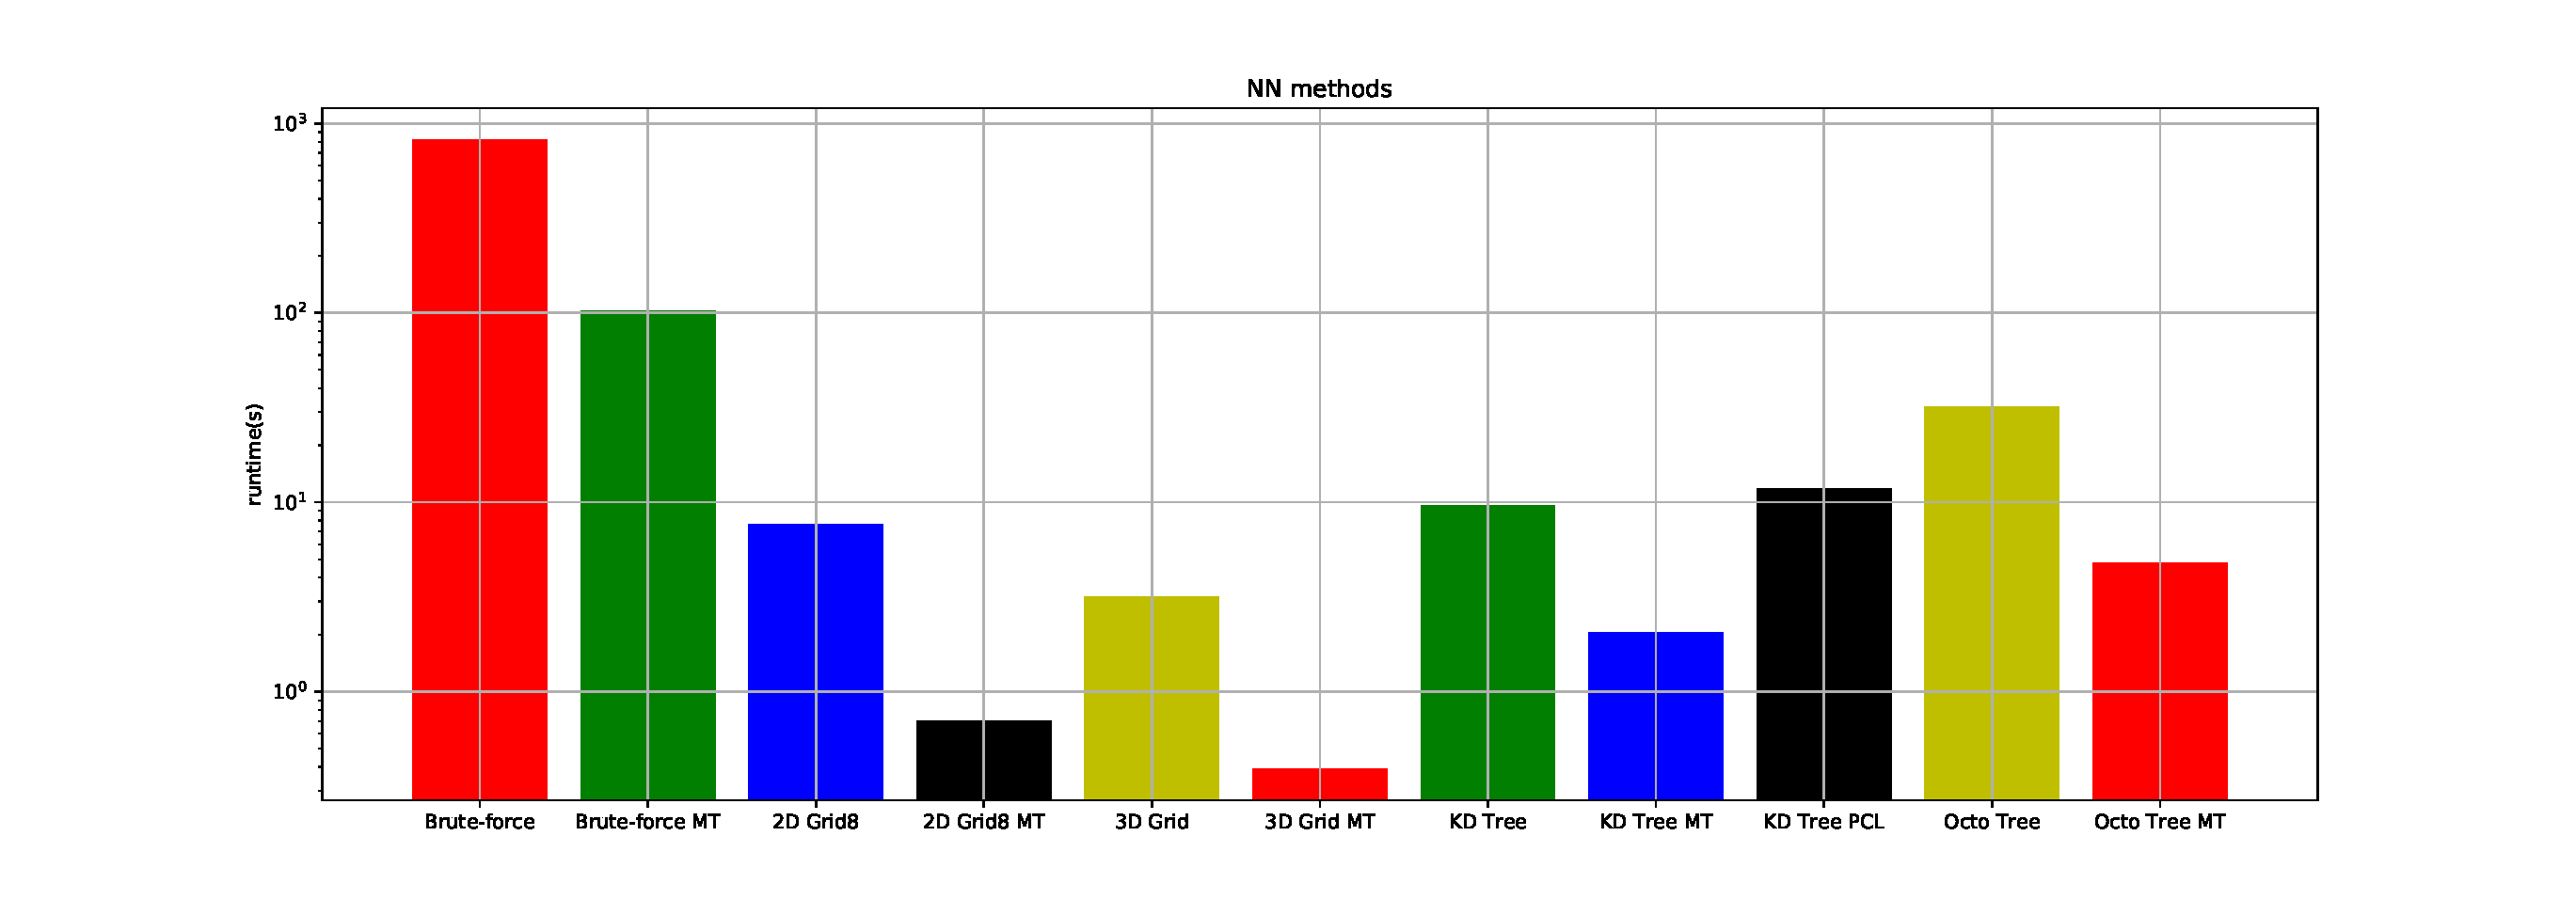
\includegraphics[width=1.0\textwidth]{resources/basic-point-cloud/nn-compare.pdf}
	\caption{Comparison of methods discussed in this section. From left to right: brute-force matching, multithreaded brute-force, 8-neighbor 2D grid, multithreaded 8-neighbor 2D grid, 3D voxel, multithreaded 3D voxel, KD-tree, multithreaded KD-tree, PCL's KD-tree, octree, and multithreaded octree. Note that due to the significantly longer computation time of brute-force matching, a logarithmic axis is used.}
	\label{fig:nn-compare}
\end{figure}

In terms of computation time, for our given dataset, 3D/2D grid-based methods performed the best, followed by K-d trees, while brute-force search was clearly the slowest. However, if the point cloud contains more points, the number of points within each grid cell will also increase, leading to linear growth in computational cost with grid cell density. Thus, grid methods are unsuitable for dense point clouds. In contrast, K-d trees exhibit logarithmic complexity growth. It can be inferred that beyond a certain scale, tree-based methods like K-d trees and octrees will become more advantageous. These tree-based approaches can also balance computation time and accuracy through approximate nearest neighbor (ANN) techniques.

\section{Fitting Problems}
Next, we introduce another important topic in point cloud processing algorithms: the extraction and estimation of basic geometric elements. Sometimes such problems are categorized as \textbf{detection} or \textbf{clustering} problems, leaning more towards perception methods. For example, many applications in autonomous driving focus heavily on extracting semantic elements like vehicles and pedestrians from point clouds. These elements can serve as data sources for subsequent decision-making and planning \cite{Navarro-Serment2010}. In SLAM, however, we are more concerned with how to use these elements to assist in \textbf{registration} between point clouds. Therefore, in traditional SLAM applications, the elements we focus on are typically basic and static, rather than dynamic or semantic. Registering a point to a plane is relatively straightforward, but registering one vehicle to another requires significantly more work\footnote{Even though the algorithm for registering two vehicles likely still relies on basic point-to-point methods.}.

In registration problems, a common approach is to first use a nearest-neighbor structure to find several nearest neighbors for a point, then fit these neighbors to a fixed geometric shape. Finally, the vehicle's pose is adjusted so that the scanned LiDAR points align with these shapes. The previous section covered various solutions to the nearest-neighbor problem, while this section focuses on extracting linear features like lines and planes from point clouds. We will see that these can be elegantly unified under the same framework (linear least squares) and solved using linear algebra.

\subsection{Plane Fitting}
As with many other problems, \textbf{linear} problems are often the simplest cases. Linear fitting of point clouds is the most basic component. The linear fitting problem for point clouds can be approached from several perspectives, and comparing these viewpoints provides different insights. The same problem may be referred to by different names across fields, yet their solutions are deeply interconnected. A linear fitting problem might be called \textbf{linear regression} (regressing the parameters of a line) or \textbf{principal component analysis (PCA)} (analyzing the primary axes of a point cloud's distribution).

Let's first consider plane fitting. Given a point cloud $\mathbf{X} = \{ \mathbf{x}_1, \ldots, \mathbf{x}_n \}$ composed of $n$ points, where each point has 3D Euclidean coordinates $\mathbf{x}_k \in \mathbb{R}^3$, we seek plane parameters $\mathbf{n}, d$ such that:
\begin{equation}
	\forall k \in [1, n], \mathbf{n}^\top \mathbf{x}_k + d = 0,
\end{equation}
where $\mathbf{n} \in \mathbb{R}^3$ is the normal vector and $d \in \mathbb{R}$ is the intercept.

Clearly, this problem has four unknowns, while each point provides one equation. With multiple points, noise typically makes the system overdetermined and unsolvable. Thus, we often seek a least squares solution (Linear Least Square) to minimize the error:
\begin{equation}
	\min_{\mathbf{n}, d} \sum_{k=1}^{n} \| \mathbf{n}^\top \mathbf{x}_k + d \|_2^2.
\end{equation}
Using homogeneous coordinates can further simplify the problem. The homogeneous coordinates of a 3D point are four-dimensional, though in practice we simply append a 1:
\begin{equation}
	\tilde{\mathbf{x}} = [\mathbf{x}^\top, 1]^\top \in \mathbb{R}^4.
\end{equation}
Thus, $\tilde{\mathbf{n}} = [\mathbf{n}^\top, d]^\top \in \mathbb{R}^4$ is also a homogeneous vector, and the problem can be rewritten as:
\begin{equation}\label{eq.6.6}
	\min_{\tilde{\mathbf{n}}} \sum_{k=1}^{n} \| \tilde{\mathbf{x}}^\top_k \tilde{\mathbf{n}} \|_2^2.
\end{equation}
The subscript 2 denotes the L2-norm (standard Euclidean norm), and the superscript 2 indicates the squared sum of norms. This is a \textbf{summation-form} linear least squares problem, which can also be expressed in matrix form. Stacking all points into a matrix:
\begin{equation}
	\tilde{\mathbf{X}} = [\tilde{\mathbf{x}}_1, \ldots, \tilde{\mathbf{x}}_n],
\end{equation}
the summation can be omitted:
\begin{equation}
	\min_{\tilde{\mathbf{n}}} \| \tilde{\mathbf{X}}^\top \tilde{\mathbf{n}} \|_2^2.
\end{equation}

This is essentially solving a linear algebra problem: given any matrix $\mathbf{A}$ (not necessarily square), we seek a non-zero vector $\mathbf{x}$ that minimizes $\mathbf{A} \mathbf{x}$. Of course, if $\mathbf{x} = 0$, the product is trivially zero, but we want non-trivial solutions, so we impose $\mathbf{x} \neq 0$. Moreover, scaling $\mathbf{x}$ by a non-zero constant $k$ scales $\mathbf{A}\mathbf{x}$ by $k$ (and its squared norm by $k^2$). Thus, we disregard the magnitude of $\mathbf{x}$ and focus on its direction by enforcing $\|\mathbf{x}\|=1$.

For $\mathbf{A}$, we impose no constraints. In the point cloud plane extraction problem, $\mathbf{A}$ is an $\mathbb{R}^{n \times 4}$ matrix, and $\mathbf{x}$ is a unit vector in $\mathbb{R}^4$. We can then ask: for which $\mathbf{x}$ does $\mathbf{A}\mathbf{x}$ attain its maximum or minimum?

Next, we will first discuss how to solve such problems in general linear algebra before returning to the plane fitting problem. Moving from the abstract to the concrete is always easier.

\subsubsection{Various Solutions to Linear Least Squares}
\paragraph{Eigenvalue Solution}
Algebraically, linear least squares refers to finding $\mathbf{x}^* \in \mathbb{R}^n$ for a given matrix $\mathbf{A} \in \mathbb{R}^{m \times n}$ such that:
\begin{equation}\label{key}
	\mathbf{x}^* = \arg \min_{\mathbf{x}} \|\mathbf{A} \mathbf{x} \|^2_2 =  \arg \min_{\mathbf{x}} \mathbf{x}^\top \mathbf{A}^\top 
	\mathbf{A} \mathbf{x}, \quad \text{s.t.}, \| \mathbf{x} \| = 1.
\end{equation}

We observe that $\mathbf{A}^\top \mathbf{A}$ is a real symmetric matrix. According to linear algebra theory, real symmetric matrices can always be diagonalized via eigenvalue decomposition:
\begin{equation}\label{key}
	\mathbf{A}^\top \mathbf{A} = \mathbf{V} \boldsymbol{\Lambda} \mathbf{V}^{-1},
\end{equation}
where $\boldsymbol{\Lambda}$ is a diagonal matrix of eigenvalues, which we assume are arranged in descending order as $\lambda_1, \ldots, \lambda_n$. $\mathbf{V}$ is an orthogonal matrix whose column vectors $\mathbf{v}_1, \ldots, \mathbf{v}_n$ are the corresponding eigenvectors, forming an orthonormal basis. Any vector $\mathbf{x}$ can be expressed as a linear combination of this basis:
\begin{equation}\label{key}
	\mathbf{x} = \alpha_1 \mathbf{v}_1 + \ldots + \alpha_n \mathbf{v}_n.
\end{equation}

It follows that\footnote{Alternatively, from the eigenvector perspective: $\mathbf{A}^\top \mathbf{A} \mathbf{x} = \sum_{k=1}^{n} \alpha_k \lambda_k \mathbf{v}_k$, yielding the same result.}:
\begin{equation}\label{key}
	\mathbf{V}^{-1} \mathbf{x} = \mathbf{V}^\top \mathbf{x} = [\alpha_1, \ldots, \alpha_n]^\top. 
\end{equation}

Thus, the objective function becomes:
\begin{equation}\label{key}
	\| \mathbf{A} \mathbf{x} \|_2^2 = \sum_{k=1}^{n} \lambda_k \alpha_k^2,
\end{equation}
with the constraint $\| \mathbf{x} \| = 1$ implying $\alpha_1^2 + \ldots + \alpha_n^2 = 1$. Since the eigenvalues $\lambda_k$ are arranged in descending order, the minimum is achieved by setting $\alpha_1 = 0, \ldots, \alpha_{n-1} = 0, \alpha_n = 1$, i.e., $\mathbf{x}^* = \mathbf{v}_n$.

We conclude that the optimal solution to the linear least squares problem is the \textbf{eigenvector corresponding to the smallest eigenvalue}. Since this problem aims to solve $\mathbf{A} \mathbf{x} = \mathbf{0}$, it can also be referred to as the \textbf{null space solution}. Note that the eigenvalue decomposition is performed on $\mathbf{A}^\top \mathbf{A}$ rather than directly on $\mathbf{A}$ (as $\mathbf{A}$ may not be diagonalizable, whereas $\mathbf{A}^\top \mathbf{A}$, being real symmetric, is guaranteed to be diagonalizable).

\paragraph{Singular Value Solution}
The aforementioned problem can also be approached from another perspective using \textbf{Singular Value Decomposition (SVD)}. Since any matrix can be decomposed via SVD, we perform SVD on $\mathbf{A}$ to obtain:
\begin{equation}\label{key}
	\mathbf{A} = \mathbf{U} \boldsymbol{\Sigma} \mathbf{V}^\top,
\end{equation}
where $\mathbf{U}$ and $\mathbf{V}$ are orthogonal matrices, and $\boldsymbol{\Sigma}$ is a diagonal matrix called the \textbf{singular value matrix}, with its diagonal elements being the singular values of $\mathbf{A}$, typically arranged in descending order.  

Substituting the SVD result into the linear least squares problem, since $\mathbf{U}$ is orthogonal, it cancels out when computing the L2-norm. We observe that this approach is essentially equivalent to the eigenvalue method:
\begin{equation}\label{key}
	\mathbf{x}^\top \mathbf{A}^\top \mathbf{A} \mathbf{x} = \mathbf{x}^\top \mathbf{V} 
	\boldsymbol{\Sigma}^2 \mathbf{V}^\top \mathbf{x}.
\end{equation}

Thus, similar to the eigenvalue solution, we take $\mathbf{x}$ as the last column of $\mathbf{V}$. In fact, the relationship between the singular values of $\mathbf{A}$ and the eigenvalues of $\mathbf{A}^\top\mathbf{A}$ is well-documented in many matrix theory textbooks \cite{Magnus1998}. Here, we take this opportunity to reintroduce this concept through a practical problem.  

Furthermore, fitting an $(N-1)$-dimensional hyperplane to points in $N$-dimensional space can also be viewed as solving the null space problem in least squares. In summary, to fit a plane to a set of points, we simply:  

\begin{enumerate}
\item Arrange all point coordinates into matrix $\mathbf{A}$,  
\item Compute the right singular vector corresponding to the smallest singular value of $\mathbf{A}$, or compute the eigenvector corresponding to the smallest eigenvalue of $\mathbf{A}^\top \mathbf{A}$.  
\end{enumerate}

Either approach yields the desired solution.

\subsection{Plane Fitting Implementation}
Let's now implement plane fitting starting from a point cloud. Most linear algebra operations can be handled using Eigen. We implement the plane fitting function in the common math library:

\begin{lstlisting}[language=c++,caption=src/common/math\_utils.h]
template <typename S>
bool FitPlane(std::vector<Eigen::Matrix<S, 3, 1>>& data, Eigen::Matrix<S, 4, 1>& plane_coeffs, double eps = 1e-2) {
	if (data.size() < 3) {
		return false;
	}
	
	Eigen::MatrixXd A(data.size(), 4);
	for (int i = 0; i < data.size(); ++i) {
		A.row(i).head<3>() = data[i].transpose();
		A.row(i)[3] = 1.0;
	}
	
	Eigen::JacobiSVD svd(A, Eigen::ComputeThinV);
	plane_coeffs = svd.matrixV().col(3);
	
	// check error eps
	for (int i = 0; i < data.size(); ++i) {
		double err = plane_coeffs.template head<3>().dot(data[i]) + plane_coeffs[3];
		if (err * err > eps) {
			return false;
		}
	}
	
	return true;
}
\end{lstlisting}

We use fast SVD decomposition, computing only the last column of the SVD result for matrix $\mathbf{A}$. After computation, we also verify the squared error against points doesn't exceed a preset threshold. Now let's write a test program that:

1. Takes randomly generated plane parameters as ground truth
2. Samples points on the plane 
3. Adds noise
4. Performs plane fitting:

\begin{lstlisting}[language=c++,caption=src/ch5/linear\_fitting.cc]
void PlaneFittingTest() {
	Vec4d true_plane_coeffs(0.1, 0.2, 0.3, 0.4);
	true_plane_coeffs.normalize();
	
	std::vector<Vec3d> points;
	
	// Generate simulated plane points randomly
	cv::RNG rng;
	for (int i = 0; i < FLAGS_num_tested_points_plane; ++i) {
		// Generate random point, compute 4th dimension, add noise, then normalize
		Vec3d p(rng.uniform(0.0, 1.0), rng.uniform(0.0, 1.0), rng.uniform(0.0, 1.0));
		double n4 = -p.dot(true_plane_coeffs.head<3>()) / true_plane_coeffs[3];
		p = p / (n4 + 1e-18);  // Prevent division by zero
		p += Vec3d(rng.gaussian(FLAGS_noise_sigma), rng.gaussian(FLAGS_noise_sigma), rng.gaussian(FLAGS_noise_sigma));
		
		points.emplace_back(p);
		
		// Verify point-to-plane error
		LOG(INFO) << "res of p: " << p.dot(true_plane_coeffs.head<3>()) + true_plane_coeffs[3];
	}
	
	Vec4d estimated_plane_coeffs;
	if (sad::math::FitPlane(points, estimated_plane_coeffs)) {
		LOG(INFO) << "estimated coeffs: " << estimated_plane_coeffs.transpose()
		<< ", true: " << true_plane_coeffs.transpose();
	} else {
		LOG(INFO) << "plane fitting failed";
	}
}
\end{lstlisting}

Now compile and run the test program to compare estimated plane parameters with ground truth:
\begin{lstlisting}[language=sh,caption=Terminal output:]
./bin/linear_fitting 
I0121 11:04:49.878834 208913 linear_fitting.cc:21] testing plane fitting
I0121 11:04:49.879319 208913 linear_fitting.cc:46] res of p: -0.00149684
I0121 11:04:49.879382 208913 linear_fitting.cc:46] res of p: -0.00221244
...
I0121 11:04:49.879462 208913 linear_fitting.cc:51] estimated coeffs: 0.186755 0.363656 0.546692 0.730757, true: 0.182574 0.365148 0.547723 0.730297
\end{lstlisting}

We can observe the difference between ground truth and estimated parameters is around 3 decimal places. Additionally, linear methods don't depend on initial values and work well even when plane point coordinates are far from the origin.

\subsection{Line Fitting}
\label{sec:line-fitting}
Let us now consider a problem very similar to plane fitting: line fitting. We still assume the point set $\mathbf{X}$ consists of $n$ 3D points. However, we can describe a straight line in several different ways, such as treating the line as the intersection of two planes, or using a point on the line plus a direction vector to define the line. The latter approach is more intuitive.

Let a point $\mathbf{x}$ on the line satisfy the equation:
\begin{equation}\label{key}
	\mathbf{x} = \mathbf{d} t + \mathbf{p},
\end{equation}
where $\mathbf{d}, \mathbf{p} \in \mathbb{R}^3$, $t \in \mathbb{R}$. Here, $\mathbf{d}$ is the direction vector of the line, satisfying $\|\mathbf{d}\| = 1$; $\mathbf{p}$ is a point on the line $l$, and $t$ is the line parameter. We aim to solve for $\mathbf{d}$ and $\mathbf{p}$, totaling 6 unknowns. Clearly, when the given point set is large, this remains an overdetermined system, requiring the construction of a least squares problem for solution.

For any point $\mathbf{x}_k$ not on $l$, we can use the Pythagorean theorem to compute the squared perpendicular distance from the point to the line:
\begin{equation}\label{key}
	f^2_k = \| \mathbf{x}_k - \mathbf{p}\|^2 - \| (\mathbf{x}_k-\mathbf{p})^\top \mathbf{d} \|^2 ,
\end{equation}
and then formulate the least squares problem to solve for $\mathbf{d}$ and $\mathbf{p}$:
\begin{equation}\label{key}
	(\mathbf{d},\mathbf{p})^* = \arg \min_{\mathbf{d}, \mathbf{p}} \sum_{k=1}^{n} f_k^2, \quad \text{s.t.} \|\mathbf{d}\|= 1.
\end{equation}
Since the error term for each point is already squared, we simply need to sum them.

Next, we separate the $\mathbf{d}$ and $\mathbf{p}$ components. First, consider $\frac{\partial f^2_k}{\partial \mathbf{p}}$:
\begin{align}\label{key}
	\frac{\partial f^2_k}{\partial \mathbf{p}} &= -2(\mathbf{x}_k - \mathbf{p}) + 2 \underbrace{(\mathbf{x}_k - \mathbf{p})^\top \mathbf{d}}_{\text{scalar, }=\mathbf{d}^\top (\mathbf{x}_k - \mathbf{p})} \mathbf{d}, \\
	&= (-2) (\mathbf{I} - \mathbf{d} \mathbf{d}^\top) (\mathbf{x}_k - \mathbf{p}).
\end{align}
Thus, the derivative of the overall objective function with respect to $\mathbf{p}$ is:
\begin{align}\label{key}
	\frac{\partial \sum_{k=1}^{n} f_k^2}{\partial \mathbf{p}} &= \sum_{k=1}^{n} (-2) (\mathbf{I} - \mathbf{d} \mathbf{d}^\top) (\mathbf{x}_k - \mathbf{p}), \\ 
	&= (-2) (\mathbf{I} - \mathbf{d} \mathbf{d}^\top) \sum_{k=1}^n (\mathbf{x}_k - \mathbf{p}).
\end{align}
To find the extremum of the least squares problem, set this equal to zero, yielding:
\begin{equation}
	\mathbf{p} = \frac{1}{n} \sum_{k=1}^n \mathbf{x}_k,
\end{equation}
indicating that $\mathbf{p}$ should be the centroid of the point cloud. Thus, we can first determine $\mathbf{p}$ and then consider $\mathbf{d}$. With $\mathbf{p}$ solved, let $\mathbf{y}_k = \mathbf{x}_k - \mathbf{p}$, treating $\mathbf{y}_k$ as known, and simplify the error term:
\begin{equation}\label{eq.6.24}
	f_k^2 = \mathbf{y}_k^\top \mathbf{y}_k - \mathbf{d}^\top \mathbf{y}_k \mathbf{y}_k^\top \mathbf{d}.
\end{equation}

Clearly, the first error term does not contain $\mathbf{d}$ and is unaffected by the choice of $\mathbf{d}$, so it can be omitted. Minimizing the second term is equivalent to maximizing its negation:
\begin{equation}\label{key}
	\mathbf{d}^* = \arg \max_{\mathbf{d}} \sum_{k=1}^{n} \mathbf{d}^\top \mathbf{y}_k\mathbf{y}_k^\top \mathbf{d} = \sum_{k=1}^{n} \| \mathbf{y}_k^\top \mathbf{d}\|_2^2.
\end{equation}
If we define:
\begin{equation}\label{key}
	\mathbf{A} = \begin{bmatrix}
		\mathbf{y}_1^\top \\
		\ldots \\
		\mathbf{y}_n^\top
	\end{bmatrix},
\end{equation}
then the problem becomes:
\begin{equation}\label{eq.6.33}
	\mathbf{d}^* = \arg \max_{\mathbf{d}} \| \mathbf{A} \mathbf{d} \|_2^2.
\end{equation}
This problem is still very similar to (\ref{eq.6.6}), except that we seek to \textbf{maximize} rather than \textbf{minimize}. For plane fitting, we minimized this problem; for line fitting, we maximize it. Following the previous discussion, taking $\mathbf{d}$ as the eigenvector corresponding to the smallest eigenvalue or singular value yields the minimizing solution; conversely, taking the eigenvector corresponding to the largest eigenvalue yields the maximizing solution. Thus, the solution to this problem should take $\mathbf{d}$ as the right singular vector corresponding to the largest singular value of $\mathbf{A}$, or the eigenvector corresponding to the largest eigenvalue of $\mathbf{A}^\top \mathbf{A}$.

\begin{figure}[!htp]
	\centering
	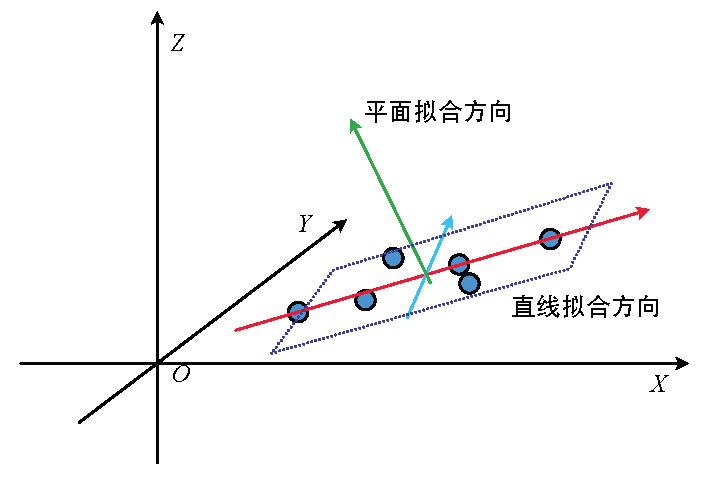
\includegraphics[width=0.5\textwidth]{resources/basic-point-cloud/linear-fitting.pdf}
	\caption{Schematic diagram of line fitting and plane fitting for point clouds`}
	\label{fig:linear-fitting}
\end{figure}
`
\subsection{Implementation of Line Fitting}
Now let's implement the line fitting method described earlier. Similarly, we first implement the fitting function in the math library, then compare the fitted results with ground truth in a test program.

\begin{lstlisting}[language=c++,caption=src/common/math\_utils.h]
template <typename S>
bool FitLine(std::vector<Eigen::Matrix<S, 3, 1>>& data, Eigen::Matrix<S, 3, 1>& origin, Eigen::Matrix<S, 3, 1>& dir,
double eps = 0.2) {
	if (data.size() < 2) {
		return false;
	}
	
	origin = std::accumulate(data.begin(), data.end(), Eigen::Matrix<S, 3, 1>::Zero().eval()) / data.size();
	
	Eigen::MatrixXd Y(data.size(), 3);
	for (int i = 0; i < data.size(); ++i) {
		Y.row(i) = (data[i] - origin).transpose();
	}
	
	Eigen::JacobiSVD svd(Y, Eigen::ComputeFullV);
	dir = svd.matrixV().col(0);
	
	// check eps
	for (const auto& d : data) {
		if (dir.template cross(d - origin).template squaredNorm() > eps) {
			return false;
		}
	}
	
	return true;
}
\end{lstlisting}

Note that we need to compute the full $\mathbf{V}$ matrix of the SVD since we want the largest singular value. The rest of the computation remains consistent with the mathematical formulation. Below is the test program:

\begin{lstlisting}[language=c++,caption=src/ch5/linear\_fitting.cc]
void LineFittingTest() {
	// Ground truth line parameters
	Vec3d true_line_origin(0.1, 0.2, 0.3);
	Vec3d true_line_dir(0.4, 0.5, 0.6);
	true_line_dir.normalize();
	
	// Generate random points along the line using parametric equation
	std::vector<Vec3d> points;
	cv::RNG rng;
	for (int i = 0; i < fLI::FLAGS_num_tested_points_line; ++i) {
		double t = rng.uniform(-1.0, 1.0);
		Vec3d p = true_line_origin + true_line_dir * t;
		p += Vec3d(rng.gaussian(FLAGS_noise_sigma), rng.gaussian(FLAGS_noise_sigma), rng.gaussian(FLAGS_noise_sigma));
		
		points.emplace_back(p);
	}
	
	Vec3d esti_origin, esti_dir;
	if (sad::math::FitLine(points, esti_origin, esti_dir)) {
		LOG(INFO) << "estimated origin: " << esti_origin.transpose() << ", true: " << true_line_origin.transpose();
		LOG(INFO) << "estimated dir: " << esti_dir.transpose() << ", true: " << true_line_dir.transpose();
	} else {
		LOG(INFO) << "line fitting failed";
	}
}
\end{lstlisting}

Similarly, we first set the ground truth line parameters, add noise to sampled points along the line, then estimate the line parameters from these samples. The test results are:

\begin{lstlisting}[language=sh,caption=Terminal output:]
	./bin/linear_fitting
	I0121 12:14:10.936178 212707 linear_fitting.cc:24] testing line fitting
	I0121 12:14:10.936190 212707 linear_fitting.cc:77] estimated origin: 0.102906 0.204955 0.305633, true: 0.1 0.2 0.3
	I0121 12:14:10.936200 212707 linear_fitting.cc:78] estimated dir:  0.45294 0.569855 0.685646, true: 0.455842 0.569803 0.683763
\end{lstlisting}

At this point, we have demonstrated how to fit lines and planes to 3D point clouds. Interestingly, these two problems share remarkable similarities and can even be reduced to \textbf{finding the maximum and minimum solutions of the same problem}, as illustrated in Figure~\ref{fig:linear-fitting}. Line fitting seeks the direction of maximum variance, while plane fitting seeks the direction of minimum variance; line fitting corresponds to the eigenvector of the largest eigenvalue, while plane fitting corresponds to the smallest eigenvalue. This aligns perfectly with our intuition.

Extending to higher or lower dimensions, the plane fitting discussed here becomes fitting an $N-1$ dimensional hyperplane to points in $N$-dimensional space, while line fitting becomes fitting a 1-dimensional subspace. When points lie in 2D space ($N=2$), plane fitting reduces to line fitting, making the two problems identical. In higher dimensions, we can pose more complex questions - for example, what form should we fit for 5D point clouds in 4D or 3D space? While these questions may sound abstract, they have practical applications in numerous cases. Of course, people typically refer to them as \textbf{data} rather than point clouds. These $N-2$, $N-3$ dimensional fittings are also called \textbf{data dimensionality reduction}, implemented through SVD decomposition by selecting different columns of the $\mathbf{V}$ matrix or eliminating components with near-zero singular values while retaining those with larger singular values. Like squeezing water from a sponge, directions with small singular values represent \textbf{noise} while those with large singular values contain the \textbf{essential information}. These methods find applications in data compression, feature extraction, and more, with different names across domains. In Principal Component Analysis (PCA) \cite{Wold1987}, they're called \textbf{maximum principal components} or \textbf{minimum principal components}. In low-rank approximation problems \cite{Eckart1936}, line fitting can be viewed as a rank-1 approximation. Alternatively, in subspace analysis \cite{Lay2005}, line fitting constructs the range space (or row/column space) while plane fitting constructs the null space. Linear problems often exhibit intricate connections, with conclusions that are universally applicable. All these problems can be modeled as linear least squares problems, with SVD or eigenvalue decomposition remaining the core solution approaches.

\section{Summary}
This chapter introduced fundamental point cloud representations and basic point cloud-related problems, such as nearest neighbor search and fitting solutions. Starting from first principles, we implemented brute-force nearest neighbor search, K-d trees, octrees, and other nearest neighbor methods, and conducted comparative experiments with PCL versions in terms of efficiency and accuracy. Since we only need to consider LiDAR point clouds without accommodating various other point cloud templates, our implementations of K-d trees and other data structures are more concise than PCL's versions. These data structures are highly useful and will be employed in subsequent chapters to implement point cloud registration, odometry, and other algorithmic modules.

\section*{Exercises}
\begin{enumerate}
	\item Define NEARBY14 in 3D voxels and implement 14-cell nearest neighbor search.
	\item Extend the K-d tree point cloud type to a template class.
	\item Incorporate bounding boxes into the K-d tree node structure to achieve more precise pruning.
	\item Attempt to improve the lower bound accuracy of the distance between query points and bounding boxes in octrees, and observe whether nearest neighbor performance improves.
	\item Derive that the solution to Equation~\eqref{eq.6.33} is the eigenvector corresponding to the largest eigenvalue of $\mathbf{A}^\top \mathbf{A}$.
	\item Compare the nearest neighbor algorithms in this chapter with common approximate nearest neighbor algorithms such as nanoflann \cite{Blanco2014}, Faiss \cite{Johnson2019}, and nmslib \cite{Boytsov2016}, and evaluate their performance in point cloud nearest neighbor search.
\end{enumerate}

% 6. 2D Lidar mapping
% !Mode:: "TeX:UTF-8"
\thispagestyle{empty}  
\chapter{2D Laser Localization and Mapping}  
\thispagestyle{empty}  
\label{cpt:2d-mapping}  
In the previous chapter, we introduced the basic principles of laser measurement, as well as the nearest neighbor and fitting methods for point clouds. These serve as the foundation for most laser point cloud registration methods. However, people often treat 2D and 3D laser processing scenarios differently. Overall, 2D laser registration is easier and more suitable for introducing image-like processing methods. This chapter will introduce the relatively simpler 2D laser SLAM, while the next chapter will cover 3D laser SLAM systems. Readers can compare the differences between the two systems from theoretical and methodological perspectives.  

\includepdf[width=\textwidth]{art/ch6.pdf}

\section{Basic Principles of 2D Laser SLAM}

\begin{figure}[!htp]  
	\centering  
	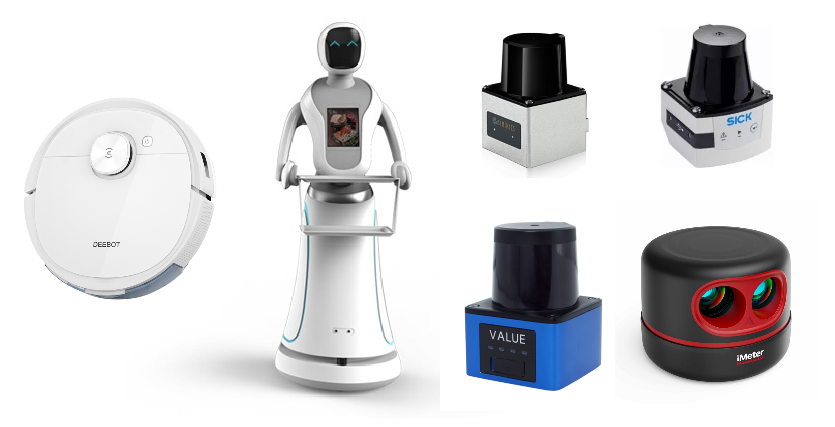
\includegraphics[width=0.8\textwidth]{resources/2d-lidar-mapping/2d-robots.pdf}  
	\caption{Robots using 2D laser SLAM and their corresponding lidars. Cleaning robots typically mount lidars on top, while service robots have built-in lidars after slotting at the base.}  
	\label{fig:2d-robots}  
\end{figure}  

All real-world sensors naturally operate in three-dimensional space, inherently without any distinction of dimensionality. However, most wheeled robots move only on a fixed plane, unlike aircraft that freely change their posture. Cleaning robots operate on horizontal ground, while wall-climbing robots work on vertical planes. Some robots, such as hotel food delivery robots, may have a certain height in their main body, but the part primarily responsible for movement—and thus the main focus of SLAM algorithms—is two-dimensional, as shown in Figure~\ref{fig:2d-robots}.  

Compared to point clouds in three-dimensional space, 2D SLAM can be viewed as a laser SLAM algorithm operating from a top-down perspective. From this viewpoint, laser scan data and map data can be simplified into two-dimensional forms. They closely resemble images, and the map itself can even be stored as an image. Some image feature extraction and matching algorithms can also be applied to 2D SLAM. 2D SLAM is crucial for applications like cleaning robots and AGVs (Automated Guided Vehicles) and was once the dominant focus of SLAM technology \cite{Thrun2005} (it remains the most widely deployed field today). Historically, it has given rise to many well-known methods, such as FastSLAM \cite{Montemerlo2002}, GMapping \cite{Grisetti2007a}, and others.  

However, due to the assumption of planar motion, when the robot body or the environment contains significant three-dimensional objects, some fundamentally unsolvable problems arise at the system level. For example, most 2D SLAM solutions assume obstacles are at the same height as the laser sensor. If the environment contains obstacles at other heights or objects whose shapes vary noticeably with height (e.g., a tabletop and its legs are clearly different), 2D maps struggle to represent such objects, and the robot may collide with them. Another example is when the robot moves on an inclined slope, where the scanned object distances differ geometrically from the actual distances. These scenarios violate the 2D motion assumption and are inherent limitations of the system, making them difficult to resolve within the framework of 2D SLAM. The 3D point cloud SLAM introduced in the next chapter can effectively address these shortcomings caused by 2D assumptions.  

On the other hand, early 2D SLAM systems often treated the map as a single 2D image, an approach that was simplistic and not well-suited for handling loop closures. This chapter will introduce 2D SLAM from a more modern perspective, adopting a framework similar to that of 3D laser SLAM. The content arrangement will also emphasize the similarities between the two.  

\begin{figure}[!htp]  
	\centering  
	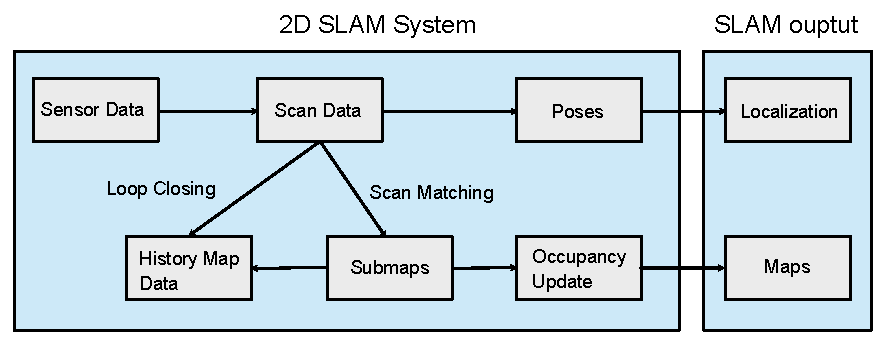
\includegraphics[width=0.8\textwidth]{resources/2d-lidar-mapping/2d-slam-pipeline.pdf}  
	\caption{The basic pipeline of submap-based 2D SLAM.}  
	\label{fig:2d-slam-pipeline}  
\end{figure}  

Figure~\ref{fig:2d-slam-pipeline}~illustrates a typical 2D SLAM framework. Here is a brief overview of its workflow:  

\begin{enumerate}  
	\item First, the 2D laser sensor outputs range measurements at a fixed frequency. Each full cycle of data is called a \textbf{scan} \footnote{Hereafter, the term "scan" will refer to the laser scan data within one cycle. Since terms like "scan-to-scan" are already widely used in the industry, we will not deliberately translate "scan."}.  
	\item To estimate the robot's pose for this scan, we need to \textbf{match} (or \textbf{register}) it against something. This process is called \textbf{scan matching}. We can match the scan either against the previous scan or against the map, so scan matching can be further divided into \textit{scan-to-scan} and \textit{scan-to-map} modes. The principles are largely the same, and they can be used flexibly in practice. In this chapter, we will implement common 2D scan matching algorithms, such as point-to-point and point-to-line methods.  
	\item After estimating the pose of this scan, we integrate it into the map. Of course, a scan is essentially a point cloud, so the simplest approach is to place all scans into the map in chronological order. However, this may suffer from cumulative errors or moving objects. Modern SLAM solutions often adopt a more flexible \textbf{submap} approach, grouping nearby laser scans into a submap and then stitching the submaps together \cite{Hess2016}. In the submap model, each submap is internally fixed and does not require repeated computation. At the same time, submaps have their own independent coordinate systems, and the poses between them can be adjusted and optimized. Thus, when handling loop closures, submaps can be treated as basic units. Early SLAM solutions often relied on a single global map \cite{Grisetti2007a}. Submaps represent an intermediate management approach between single frames and a full map, making loop closure detection and map updates more convenient. This chapter will also adopt the submap model for map construction.  
	\item Finally, how should the scanned map be stored and updated? Many robot maps need to distinguish between \textbf{obstacles} and \textbf{navigable areas}. To represent these concepts, we will use an \textbf{occupancy grid map} for map management \cite{Thrun2003a, MeyerDelius2012}. Occupancy grid maps can effectively filter out the impact of moving objects, resulting in cleaner maps.  
\end{enumerate}  

In this chapter, we will work with readers to implement the mainstream 2D SLAM algorithms discussed above. We will implement several key scan matching algorithms, build them into local submaps, and then use loop closure corrections to construct a complete occupancy grid map. Among the algorithms mentioned here, scan matching is the core of many subsequent processes. We can use traditional methods like the Iterative Closest Point (ICP) algorithm for scan matching or leverage the characteristics of 2D to implement image-based methods such as Gaussian likelihood fields.

\section{Scan Matching Algorithms}  
\subsection{Point-to-Point Scan Matching}  

Let us begin by introducing the scan matching methods in 2D SLAM. A single 2D scan is represented by a set of angle-distance pairs, denoted as $(\rho, r)_i$, where $\rho$ is the angle relative to the robot's own frame, $r$ is the measured distance, and $i = 0, \ldots N$ indicates multiple measurement points. The value of $N$ depends on the angular resolution of the laser sensor. In implementation, these data points are often stored in an array. These measurements are in polar coordinates and can be naturally converted to Cartesian coordinates, expressed as $(x,y)_i$.  

\subsubsection{Visualizing 2D Lidar Data Using OpenCV}  

Starting from this chapter, we will use real-world data collected from actual robots to verify whether our algorithms perform satisfactorily in real-world scenarios. This section and subsequent chapters will require some ROS bag files. Due to their large size, readers are advised to download the necessary datasets from the code repository associated with this book. If storage space is limited, you may choose to download only representative datasets for each chapter. The program in this section requires the data package located in the `2dmapping/` directory, while other chapters will use datasets from their respective directories.  

To facilitate testing different algorithms across various datasets, we have implemented an abstract interface for ROS bag processing. Readers only need to define callback functions for different message types. For example, in the demo code shown here, we need to read 2D scan messages from the bag file and pass them to a visualization program for rendering. In other chapters, these data may be fed into matching algorithms for registration. We leverage C++ lambda functions to achieve this flexible invocation:  

\begin{lstlisting}[language=c++,caption=src/ch6/test\_2dlidar\_io.cc]  
sad::RosbagIO rosbag_io(FLAGS_bag_path);  
rosbag_io  
.AddScan2DHandle("/pavo_scan_bottom",  
	[](Scan2d::Ptr scan) {  
		cv::Mat image;  
		sad::Visualize2DScan(scan, SE2(), image, Vec3b(255, 0, 0));  
		cv::imshow("scan", image);  
		cv::waitKey(20);  
		return true;  
	})  
.Go();  

void Visualize2DScan(Scan2d::Ptr scan, const SE2& pose, cv::Mat& image, const Vec3b& color, int image_size, float resolution, const SE2& pose_submap) {  
	if (image.data == nullptr) {  
		image = cv::Mat(image_size, image_size, CV_8UC3, cv::Vec3b(255, 255, 255));  
	}  
	
	for (size_t i = 0; i < scan->ranges.size(); ++i) {  
		if (scan->ranges[i] < scan->range_min || scan->ranges[i] > scan->range_max) {  
			continue;  
		}  
		
		double real_angle = scan->angle_min + i * scan->angle_increment;  
		double x = scan->ranges[i] * std::cos(real_angle);  
		double y = scan->ranges[i] * std::sin(real_angle);  
		
		if (real_angle < scan->angle_min + 30 * M_PI / 180.0 || real_angle > scan->angle_max - 30 * M_PI / 180.0) {  
			continue;  
		}  
		
		Vec2d psubmap = pose_submap.inverse() * (pose * Vec2d(x, y));  
		
		int image_x = int(psubmap[0] * resolution + image_size / 2);  
		int image_y = int(psubmap[1] * resolution + image_size / 2);  
		if (image_x >= 0 && image_x < image.cols && image_y >= 0 && image_y < image.rows) {  
			image.at<cv::Vec3b>(image_y, image_x) = cv::Vec3b(color[0], color[1], color[2]);  
		}  
	}  
	
	// Draw the robot's position  
	Vec2d pose_in_image =  
	pose_submap.inverse() * (pose.translation()) * double(resolution) + Vec2d(image_size / 2, image_size / 2);  
	cv::circle(image, cv::Point2f(pose_in_image[0], pose_in_image[1]), 5, cv::Scalar(color[0], color[1], color[2]), 2);  
}  
\end{lstlisting}  

As shown, this program uses the `sad::RosbagIO` class to read the `pavo_scan_bottom` messages from the bag file and passes them to a visualization function. The visualization function converts the lidar's range and angle measurements into Cartesian coordinates and renders them onto an image at a specified resolution. If the robot's pose is provided, the visualization can also display the scan data in motion. Here, we demonstrate the scan data in the robot's body frame by setting the input pose to the origin.

Now, please compile the `test_2dlidar_io` program and run the following command to view the laser scan data in the given bag file:

\begin{lstlisting}[language=sh, caption=Terminal command]
	/bin/test_2dlidar_io --bag_path ./dataset/sad/2dmapping/floor1.bag
\end{lstlisting}

Readers should see laser scan data similar to Figure~\ref{fig:2dscan}. Since the actual robot was moving, you should also observe structures from different locations in the scene. With good spatial imagination, one should be able to infer the robot's movement direction and surrounding environment.

\begin{figure}[!htp]
	\centering
	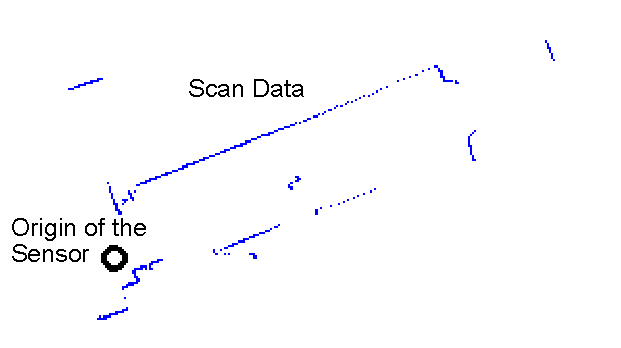
\includegraphics[width=0.5\textwidth]{resources/2d-lidar-mapping/2dscan}
	\caption{Example of single 2D scan data}
	\label{fig:2dscan}
\end{figure}

In scan data like Figure~\ref{fig:2dscan}, we call the actual laser hit points \textbf{end points}. End points have two physical meanings:
1. The end point itself represents an actual existing obstacle;
2. Along the line connecting the sensor to the end point, no other obstacles exist.

Note that the second meaning requires calculating the line from the sensor to the end point (the sensor doesn't measure this line - it only measures the end point, so we need to compute this line ourselves). If we want to calculate which grid cells this line passes through, it involves \textbf{ray casting algorithm} \cite{Ray1999} and \textbf{rasterization algorithm} \cite{Pineda1988}. We'll mention these again later in grid map construction and provide a simple implementation. However, in scan matching algorithms, we focus more on the first meaning and often ignore the second.

Under this premise, a single scan can be viewed as a simple 2D point set.

Now let us derive the mathematical model for scan matching algorithms. From the perspective of state estimation, 2D laser scan data can be denoted as observation data $\mathbf{z}$. It is obtained when the robot at pose $\mathbf{x}$ observes a certain map $\mathbf{m}$. Thus, the observation model can be simply expressed as:
\begin{equation}\label{key}
	\mathbf{z} = \mathbf{h} (\mathbf{x}, \mathbf{m}) + \mathbf{w},
\end{equation}
where $\mathbf{w}$ is the noise term. Our goal is to estimate $\mathbf{x}$ based on the observed $\mathbf{z}$ and $\mathbf{m}$. According to Bayesian estimation theory, $\mathbf{x}$ can be obtained through \textbf{Maximum a Posteriori} (MAP) or \textbf{Maximum Likelihood Estimation} (MLE):
\begin{equation}\label{key}
	\mathbf{x}_{\mathrm{MLE}} = \arg \max p(\mathbf{x}|\mathbf{z}, \mathbf{m}) = \arg \max p(\mathbf{z}|\mathbf{x}, \mathbf{m}).
\end{equation}

If we only consider the scan-to-scan problem, $\mathbf{m}$ can simply be written as the previous scan data. The key then becomes how to define the detailed form of the observation equation, i.e., how to compute the residual term for each observation. Here we present several typical solutions: point-to-point scan matching (ICP) \cite{Arun1987}, point-to-line scan matching (PL-ICP \cite{Censi2008} or ICL \cite{Alshawa2007}), and the Gaussian likelihood field method (or CSM \cite{Olson2009}). In 3D matching algorithms, we will further introduce other methods such as point-to-plane \cite{Park2003,Low2004} and NDT \cite{Biber2003,Magnusson2009,Rapp2015}. Since 2D scan matching does not involve surface elements, we will only discuss point-to-point and point-to-line algorithms here.

The specific definition of the observation equation involves several issues:
\begin{enumerate}
	\item How to select the points to be matched. In principle, all scanned points should participate in matching, but for efficiency considerations, \textbf{sampling} can be applied. There are many sampling methods, from uniform or random sampling to normal- or feature-based sampling, all of which can be used in practice.
	\item How to determine which specific map point corresponds to a scan point $(x,y)_i$. This is also known as the \textbf{data association} problem. This problem is typically solved using the nearest neighbor method introduced in the previous section, i.e., assuming that under the current estimated pose, the closest map point to the observed point is the matching point. In field-based methods, grid cells or fields in the map can also be used as matching points.
	\item After determining the scan point $(x,y)_i$ and its corresponding map point $\mathbf{m}_i$, how to compute the residual. This involves the modeling of residuals. The complete laser scan noise model (beam model) is complex with many parameters \cite{Cabaleiro2015}, and as a state estimation model, it is not smooth enough. In practice, we usually simplify it, and in the simplest case, we can directly model it as a 2D Gaussian distribution, i.e., $\mathbf{w} \sim \mathcal{N}(\mathbf{0}, \boldsymbol{\Sigma})$.
\end{enumerate}

As can be seen, a scan matching algorithm involves many choices at different stages, and there are numerous variants of basic methods in both industry and academia. We will introduce the origins of these variants starting from basic methods, but we will not attempt to cover all scan matching algorithms. To maintain consistency, we will use the same mathematical notation to describe the problems and provide code implementations for each algorithm.

First, let us look at the simplest point-to-point matching problem, also known as the Iterative Closest Point (ICP) algorithm \cite{Besl1992}. The ICP algorithm divides the scan matching problem into two steps: \textbf{data association} and \textbf{pose estimation}, and alternates between these two steps until convergence. In fact, regardless of how data association and pose estimation are specifically solved, as long as the algorithm involves alternating between these two steps, we can refer to it as an \textbf{ICP-like} algorithm \cite{Koide2020,segal2009generalized,Zhang2021a}. When the matching relationship is known, ICP can be solved in closed form, but this approach discards the possibility of further filtering outliers and makes point-to-point and point-to-plane methods appear different (note that from an optimization perspective, they are unified). For consistency, we will describe the problem in terms of residuals and optimization.

The pose of a 2D laser is described by translation and rotation angles\footnote{In the program, we use the SE2 interface, which is essentially the same as the SE3 interface. We can use the same notation for SE3 and SE2, such as matrix multiplication. In some literature, 2D poses are also referred to as \textbf{three-degree-of-freedom} poses.}, and can be simply written as:
\begin{equation}\label{key}
	\mathbf{x} = [x, y, \theta]^\top.
\end{equation}

Here, $\mathbf{x}$ describes a transformation from the robot's coordinate frame $B$ to the world frame $W$, denoted as $\mathbf{x} = \mathbf{T}_{WB}$ according to the convention of this book. Note that submap frames and their coordinate systems will be introduced later, so it is necessary to clarify the transformation relationship of $\mathbf{x}$. Suppose a scan point $\mathbf{p}_i^B$ in the robot's frame has distance and angle $r_i, \rho_i$. Then, based on the current laser pose, it can be transformed to the world frame:
\begin{equation}\label{key}
	\mathbf{p}^W_i = [x+r_i \cos (\rho_i + \theta), y+r_i \sin(\rho_i + \theta)]^\top.
\end{equation}
In 3D space, this can be written as:
\begin{equation}\label{key}
	\mathbf{p}^W_i = \mathbf{T}_{WB} \mathbf{p}^B_i.
\end{equation}

In the program, since the SE3 and SE2 interfaces are consistent, we do not deliberately distinguish between 3D and 2D poses in mathematical notation.

Assuming we find a nearest neighbor $\mathbf{q}_i^W$ near $\mathbf{p}_i^W$, we can easily construct the residual between $\mathbf{p}_i^W$ and $\mathbf{q}_i^W$:
\begin{equation}\label{key}
	\mathbf{e}_i = \mathbf{p}_i^W - \mathbf{q}_i^W,
\end{equation}

This residual describes the Euclidean geometric distance between two points. Clearly, this error uses world coordinates and is related to the robot's pose at that time. Thus, the robot pose estimation problem can be transformed into a least-squares problem with variables $x, y, \theta$:
\begin{equation}\label{key}
	(x,y,\theta)^* = \arg \min\limits_{\mathbf{x}} \sum_{i=1}^n \| \mathbf{e}_i \|_2^2.
\end{equation}
This least-squares problem can be solved by many existing solvers.

To solve the least-squares problem, we should provide the derivatives of $\mathbf{e}$ with respect to each state variable. The obvious advantage of 2D poses is that we no longer need to use manifold notation and can directly use the decomposed $x, y, \theta$\footnote{Of course, it is possible to unify them using manifold notation, but it is unnecessary.}. Based on the above definitions, we can easily obtain:
\begin{subequations}\label{key}
	\begin{align}
		\frac{\partial{\mathbf{e}_i}}{\partial x} &= [1, 0]^\top, \\
		\frac{\partial{\mathbf{e}_i}}{\partial y} &= [0, 1]^\top, \\
		\frac{\partial{\mathbf{e}_i}}{\partial \theta} &= [-r_i \sin (\rho_i + \theta), r_i \cos (\rho_i+\theta)]^\top.
	\end{align}
\end{subequations}

We can organize this into matrix form:
\begin{equation}\label{eq:dpw-dx}
	\frac{\partial \mathbf{e}_i}{\partial \mathbf{x}} = \begin{bmatrix}
		1 & 0\\
		0 & 1\\
		-r_i \sin (\rho_i + \theta) & r_i \cos (\rho_i+\theta)
	\end{bmatrix} \in \mathbb{R}^{3\times 2}.
\end{equation}

In the subsequent experimental section, we will use this Jacobian matrix to solve the Gauss-Newton method. It is important to note that if the state variables $x, y, \theta$ change, $\mathbf{q}_i$ will also change, altering the entire problem. If the state variables are initially set far from the optimal solution, $\mathbf{q}_i$ may be an incorrect point, making ICP-like methods highly dependent on the initial value of optimization. We will continue to discuss this issue later.

\subsection{Implementation of Point-to-Point ICP (Gauss-Newton)}  
Below we implement a 2D point-to-point ICP method by manually coding the Gauss-Newton approach. In each Gauss-Newton iteration, we recompute the nearest neighbors between points and then solve for the pose increment. The key points here are: (1) implementing nearest neighbor search, and (2) implementing Gauss-Newton iteration.  

Since the nearest neighbor data structure from the previous lecture used 3D points rather than 2D points, here we employ PCL's K-d tree for nearest neighbor search with 2D points. Thus, when setting the target point cloud, we need to build a K-d tree for it. Our 2D ICP class interface is as follows:  

\begin{lstlisting}[language=c++,caption=src/ch6/icp\_2d.h]  
class Icp2d {  
	public:  
	using Point2d = pcl::PointXY;  
	using Cloud2d = pcl::PointCloud<Point2d>;  
	Icp2d() {}  
	
	/// Set the target scan  
	void SetTarget(Scan2d::Ptr target) {  
		target_scan_ = target;  
		BuildTargetKdTree();  
	}  
	
	/// Set the source scan to be aligned  
	void SetSource(Scan2d::Ptr source) { source_scan_ = source; }  
	
	/// Perform alignment using Gauss-Newton method  
	bool AlignGaussNewton(SE2& init_pose);  
	
	private:  
	// Build K-d tree for the target point cloud  
	void BuildTargetKdTree();  
	
	pcl::search::KdTree<Point2d> kdtree_;  
	Cloud2d::Ptr target_cloud_;  // Target cloud in PCL format  
	
	Scan2d::Ptr target_scan_ = nullptr;  
	Scan2d::Ptr source_scan_ = nullptr;  
};  
\end{lstlisting}  

The `AlignGaussNewton` function implements 2D ICP based on Gauss-Newton iteration:  

\begin{lstlisting}[language=c++, caption=src/ch6/icp\_2d.cc]  
bool Icp2d::AlignGaussNewton(SE2& init_pose) {  
	int iterations = 10;  
	double cost = 0, lastCost = 0;  
	SE2 current_pose = init_pose;  
	const float max_dis2 = 0.01;      // Maximum squared distance for nearest neighbors  
	const int min_effect_pts = 20;  // Minimum number of effective points  
	
	for (int iter = 0; iter < iterations; ++iter) {  
		Mat3d H = Mat3d::Zero();  
		Vec3d b = Vec3d::Zero();  
		cost = 0;  
		
		int effective_num = 0;  // Number of effective points  
		
		// Traverse source points  
		for (size_t i = 0; i < source_scan_->ranges.size(); ++i) {  
			float r = source_scan_->ranges[i];  
			if (r < source_scan_->range_min || r > source_scan_->range_max) {  
				continue;  
			}  
			
			float angle = source_scan_->angle_min + i * source_scan_->angle_increment;  
			float theta = current_pose.so2().log();  
			Vec2d pw = current_pose * Vec2d(r * std::cos(angle), r * std::sin(angle));  
			Point2d pt;  
			pt.x = pw.x();  
			pt.y = pw.y();  
			
			// Nearest neighbor search  
			std::vector<int> nn_idx;  
			std::vector<float> dis;  
			kdtree_.nearestKSearch(pt, 1, nn_idx, dis);  
			
			if (nn_idx.size() > 0 && dis[0] < max_dis2) {  
				effective_num++;  
				Mat32d J;  
				J << 1, 0, 0, 1, -r * std::sin(angle + theta), r * std::cos(angle + theta);  
				H += J * J.transpose();  
				
				Vec2d e(pt.x - target_cloud_->points[nn_idx[0]].x, pt.y -  
				target_cloud_->points[nn_idx[0]].y);  
				b += -J * e;  
				
				cost += e.dot(e);  
			}  
		}  
		
		if (effective_num < min_effect_pts) {  
			return false;  
		}  
		
		// Solve for dx  
		Vec3d dx = H.ldlt().solve(b);  
		if (isnan(dx[0])) {  
			break;  
		}  
		
		cost /= effective_num;  
		if (iter > 0 && cost >= lastCost) {  
			break;  
		}  
		
		LOG(INFO) << "iter " << iter << " cost = " << cost << ", effect num: " << effective_num;  
		
		current_pose.translation() += dx.head<2>();  
		current_pose.so2() = current_pose.so2() * SO2::exp(dx[2]);  
		lastCost = cost;  
	}  
	
	init_pose = current_pose;  
	LOG(INFO) << "estimated pose: " << current_pose.translation().transpose()  
	<< ", theta: " << current_pose.so2().log();  
	
	return true;  
}  
\end{lstlisting}  

The Jacobian matrix here corresponds to the theoretical part introduced earlier. We limit the maximum squared distance for nearest neighbors (set to 0.01) and count the number of valid nearest neighbors, then compute their average error. Finally, the `current_pose` obtained from Gauss-Newton iteration is filled into the return result.

We also write a test program to evaluate the results of 2D ICP:

\begin{lstlisting}[language=c++,caption=src/ch6/test\_2d\_icp\_s2s.cc]
rosbag_io.AddScan2DHandle("/pavo_scan_bottom",
[&](Scan2d::Ptr scan) {
	current_scan = scan;
	
	if (last_scan == nullptr) {
		last_scan = current_scan;
		return true;
	}
	
	sad::Icp2d icp;
	icp.SetTarget(last_scan);
	icp.SetSource(current_scan);
	
	SE2 pose;
	if (FLAGS_method == "point2point") {
		icp.AlignGaussNewton(pose);
	} else if (fLS::FLAGS_method == "point2plane") {
		icp.AlignGaussNewtonPoint2Plane(pose);
	}
	
	cv::Mat image;
	sad::Visualize2DScan(last_scan, SE2(), image, Vec3b(255, 0, 0));    // target in blue
	sad::Visualize2DScan(current_scan, pose, image, Vec3b(0, 0, 255));  // source in red
	cv::imshow("scan", image);
	cv::waitKey(20);
	
	last_scan = current_scan;
	return true;
})
.Go();
\end{lstlisting}

This program registers the current scan data to the previous scan and visualizes the results using OpenCV. The previous frame is displayed in blue, while the current frame is shown in red. After registration, the two scans should align well with each other. Running this program allows real-time observation of the registration effect, as shown in Figure~\ref{fig:2dicp-s2s}. Readers can also monitor metrics such as the objective function value and the number of valid points for each ICP iteration in the terminal. However, due to the robot's motion, there will inevitably be some discrepancies between the two scans. Previously unexplored areas will appear in the current frame, and dynamic objects or motion distortion in the scan data itself may also interfere with the registration results. We can adjust the thresholds in ICP or parameters in the optimization model to mitigate the impact of dynamic objects to some extent.

This test program is also compatible with the point-to-plane ICP interface discussed later. Readers can use different gflags to test it.

\begin{figure}[!htp]
	\centering
	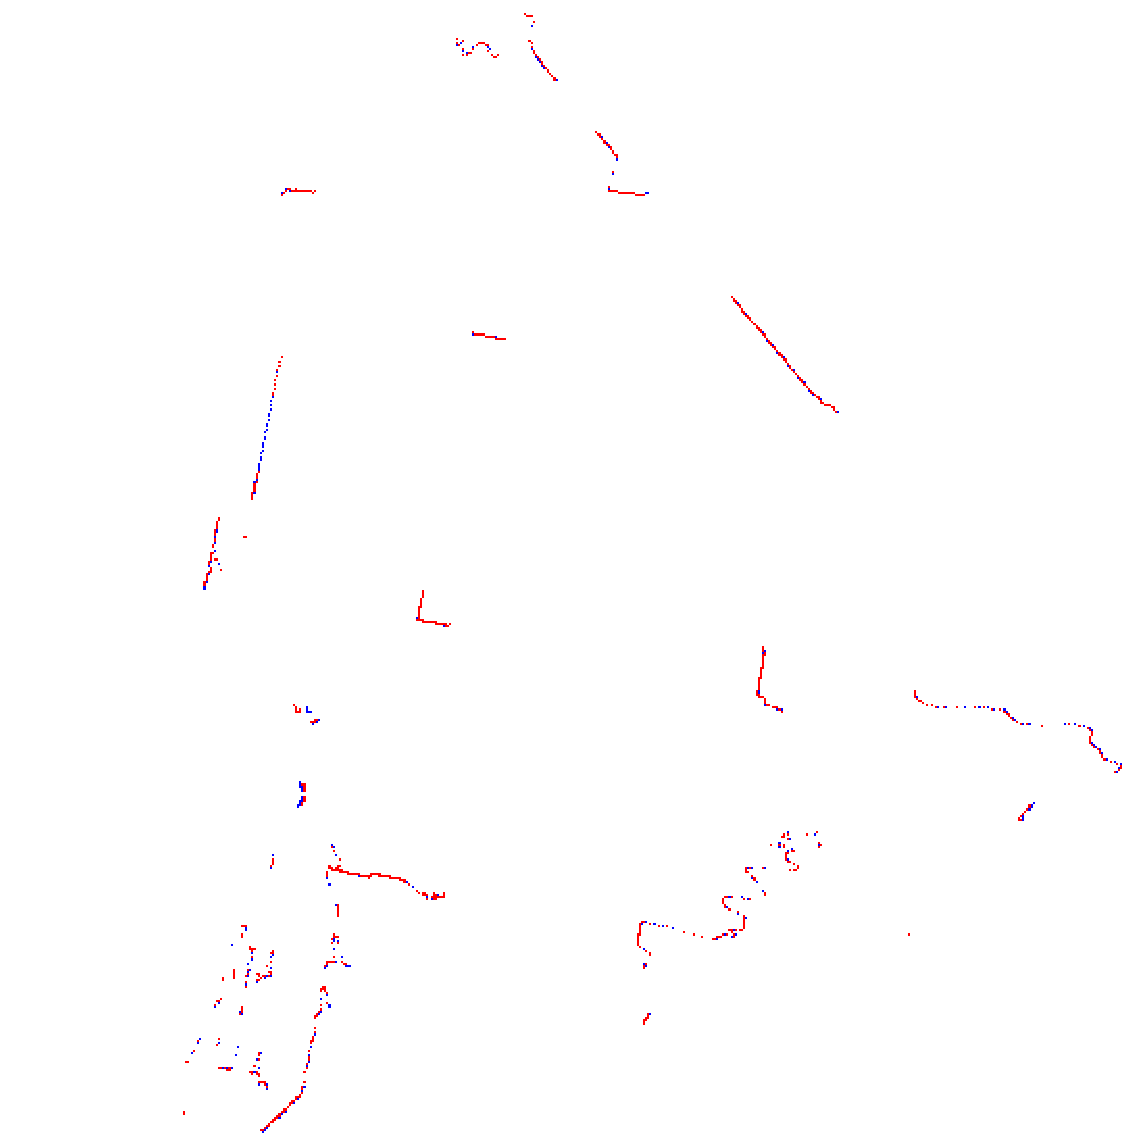
\includegraphics[width=0.4\textwidth]{resources/2d-lidar-mapping/2dicp-s2s}
	\caption{Registration results of point-to-point ICP}
	\label{fig:2dicp-s2s}
\end{figure}

\subsection{Point-to-Line Scan Matching}  
In addition to point-to-point methods, ICP can also utilize other error formulations. The most common alternatives are point-to-line or point-to-plane approaches. Since 2D lidar data doesn't contain planes, we focus on the point-to-line formulation (which can be considered a lower-dimensional version of point-to-plane). The overall workflow of point-to-line ICP remains similar to point-to-point ICP, except that during nearest neighbor search, we need to find multiple neighbors (e.g., k neighbors), fit a line to these points, and then compute the perpendicular distance from the target point to this line. This method is called Point-to-line ICP (PL-ICP) \cite{Censi2008}.

Let these k nearest neighbors be $(\mathbf{x}_1, \ldots, \mathbf{x}_k), \forall i \in 1, \ldots k, \mathbf{x}_i \in \mathbb{R}^2$. In 3D space, the fitted line can be described by a direction vector $\mathbf{d}$ and origin $\mathbf{p}$, with fitting methods already introduced in Section~\ref{sec:line-fitting}. While lines in 3D space are more complex, in 2D space they can be simplified to a slope-intercept model. Let the line equation be:
\begin{equation}\label{key}
	a x + by + c = 0,
\end{equation}
where $a,b,c$ are line parameters. The line fitting can then be formulated as a least-squares parameter estimation problem:
\begin{equation}\label{key}
	(a,b,c)^* = \arg \min \sum_{i=1}^N \| a x_i + by_i + c \|_2^2 .
\end{equation}

We simply arrange the point coordinates into a matrix:
\begin{equation}\label{key}
	\mathbf{A} = \begin{bmatrix}
		x_1 & y_1 & 1 \\
		x_2 & y_2 & 1 \\
		& \ldots &\\
		x_k & y_k & 1
	\end{bmatrix},
\end{equation}
and find the minimum singular vector of $\mathbf{A}$.

After obtaining the line parameters $(a,b,c)$ from the nearest neighbors, the perpendicular distance from any point $(x,y)$ to this line can be expressed as:
\begin{equation}\label{key}
	d = \frac{ax+by+c}{\sqrt{a^2+b^2}}.
\end{equation}
Since the denominator is a constant that can be ignored, we can directly use the residual:
\begin{equation}\label{key}
	e = ax+by+c,
\end{equation}
as the objective function. The line equation also provides the corresponding Jacobian matrix:
\begin{equation}\label{key}
	\frac{\partial e}{\partial x} = a, \quad \frac{\partial e}{\partial y} = b.
\end{equation}
Thus, the fitted line results can guide the optimization direction. We will see similar results in 3D point-to-plane ICP later.

Now we incorporate the lidar's pose into the above discussion. Let the lidar's position and orientation be $\mathbf{x} = (x,y, \theta)$. For a lidar point with distance and angle $(r_i, \rho_i)$, we transform it to world coordinates to get $\mathbf{p}_i^w$. With line parameters $(a_i, b_i, c_i)$ fitted from its nearest neighbors, the Jacobian matrix of its residual $e_i$ with respect to the pose can be expressed using the chain rule:
\begin{equation}\label{key}
	\frac{\partial e_i}{\partial \mathbf{x}} = \frac{\partial e_i}{\partial \mathbf{p}_i^w} \frac{\partial \mathbf{p}_i^w}{\partial \mathbf{x}},
\end{equation} 
where the latter term is given in Equation \eqref{eq:dpw-dx}, and the former term is determined by the line parameters. Multiplying them together yields:
\begin{equation}\label{key}
	\frac{\partial e_i}{\partial \mathbf{x}} = [a_i, b_i, -a_i r_i \sin(\rho_i + \theta) + b_i r_i \cos(\rho_i + \theta)]^\top.
\end{equation}


\subsection{Implementation of Point-to-Line ICP (Gauss-Newton)}
Below we implement the algorithm described in the previous section. Its overall workflow is consistent with point-to-point ICP, and we only need to add an interface to the existing ICP class:

\begin{lstlisting}[language=c++,caption=src/ch6/icp\_2d.cc]
	bool Icp2d::AlignGaussNewtonPoint2Plane(SE2& init_pose) {
		int iterations = 10;
		double cost = 0, lastCost = 0;
		SE2 current_pose = init_pose;
		const float max_dis = 0.3;      // Maximum distance for nearest neighbors
		const int min_effect_pts = 20;  // Minimum number of effective points
		
		for (int iter = 0; iter < iterations; ++iter) {
			Mat3d H = Mat3d::Zero();
			Vec3d b = Vec3d::Zero();
			cost = 0;
			
			int effective_num = 0;  // Number of effective points
			
			// Traverse source points
			for (size_t i = 0; i < source_scan_->ranges.size(); ++i) {
				float r = source_scan_->ranges[i];
				if (r < source_scan_->range_min || r > source_scan_->range_max) {
					continue;
				}
				
				float angle = source_scan_->angle_min + i * source_scan_->angle_increment;
				float theta = current_pose.so2().log();
				Vec2d pw = current_pose * Vec2d(r * std::cos(angle), r * std::sin(angle));
				Point2d pt;
				pt.x = pw.x();
				pt.y = pw.y();
				
				// Find 5 nearest neighbors
				std::vector<int> nn_idx;
				std::vector<float> dis;
				kdtree_.nearestKSearch(pt, 5, nn_idx, dis);
				
				std::vector<Vec2d> effective_pts;  // Effective points
				for (int j = 0; j < nn_idx.size(); ++j) {
					if (dis[j] < max_dis) {
						effective_pts.emplace_back(
						Vec2d(target_cloud_->points[nn_idx[j]].x, target_cloud_->points[nn_idx[j]].y));
					}
				}
				
				if (effective_pts.size() < 3) {
					continue;
				}
				
				// Fit line and assemble J, H and error
				Vec3d line_coeffs;
				if (math::FitLine2D(effective_pts, line_coeffs)) {
					effective_num++;
					Vec3d J;
					J << line_coeffs[0], line_coeffs[1],
					-line_coeffs[0] * r * std::sin(angle + theta) + line_coeffs[1] * r * std::cos(angle + theta);
					H += J * J.transpose();
					
					double e = line_coeffs[0] * pw[0] + line_coeffs[1] * pw[1] + line_coeffs[2];
					b += -J * e;
					
					cost += e * e;
				}
			}
			
			if (effective_num < min_effect_pts) {
				return false;
			}
			
			// solve for dx
			Vec3d dx = H.ldlt().solve(b);
			if (isnan(dx[0])) {
				break;
			}
			
			cost /= effective_num;
			if (iter > 0 && cost >= lastCost) {
				break;
			}
			
			LOG(INFO) << "iter " << iter << " cost = " << cost << ", effect num: " << effective_num;
			
			current_pose.translation() += dx.head<2>();        current_pose.so2() = current_pose.so2() * 
			SO2::exp(dx[2]);
			lastCost = cost;
		}
		
		init_pose = current_pose;
		LOG(INFO) << "estimated pose: " << current_pose.translation().transpose()
		<< ", theta: " << current_pose.so2().log();
		
		return true;
	}
\end{lstlisting}

In the implementation, we search for five nearest neighbors around the target point and use them to fit a local line segment. The 2D line fitting algorithm is provided in common/math\_utils.h:

\begin{lstlisting}[language=c++,caption=src/common/math\_utils.h]
	template <typename S>
	bool FitLine2D(const std::vector<Eigen::Matrix<S, 2, 1>>& data, Eigen::Matrix<S, 3, 1>& coeffs) {
		if (data.size() < 2) {
			return false;
		}
		
		Eigen::MatrixXd A(data.size(), 3);
		for (int i = 0; i < data.size(); ++i) {
			A.row(i).head<2>() = data[i].transpose();
			A.row(i)[2] = 1.0;
		}
		
		Eigen::JacobiSVD svd(A, Eigen::ComputeThinV);
		coeffs = svd.matrixV().col(2);
		return true;
	}
\end{lstlisting}

Note its similarity to the 3D plane fitting algorithm. Finally, the test case from the previous section can be used to examine the registration effect of point-to-line ICP. Since its results are similar to point-to-point ICP, we won't include additional figures here - readers are encouraged to experiment themselves (using the test program from the previous section with --method=point2plane). Generally speaking, point-to-line ICP performs better than point-to-point ICP, though at the cost of greater computational requirements due to the need to compute multiple nearest neighbors.

\subsection{Likelihood Field Method}
\label{sec:likelihood-field}

Point-to-point or point-to-line ICP can be used for both scan-to-scan matching and scan-to-map registration. If we store the map as discrete 2D points, ICP-like methods can be applied to map matching in the same way. However, in 2D SLAM, we typically store the map as an \textbf{occupancy grid map} with a certain resolution. This image-like map has an update mechanism that provides some filtering effect against dynamic objects (which we will implement in the next section). Thus, we can design a registration method that aligns scan data with grid maps in an ICP-like manner. The likelihood field method (also known as Gaussian Likelihood Field) introduced in this section is precisely such an approach for registering scan data with grid maps \cite{Thrun2005}.

In point-to-point ICP, we compute Euclidean distance errors between target points and their nearest neighbors in another point cloud. These errors grow with the squared distance between points and ultimately form the objective function through summation. Intuitively, we can imagine a \textbf{spring} installed between each point and its nearest neighbor. The collective pull of these springs eventually brings the point cloud to the position of minimum energy. However, in ICP methods, we must reinstall these springs during each iteration, which is computationally expensive. 

An alternative approach is to consider that the point cloud generates a \textbf{field} in space rather than installing springs between points. This field attracts nearby point clouds, with its attractive force decaying quadratically with distance. This is essentially the idea behind the likelihood field method. We can define a decaying field around each point in the map. Unlike physical fields, however, the fields in computer programs have defined \textbf{effective ranges} and \textbf{resolutions}. The field can decay quadratically or follow a Gaussian distribution with distance. When a measured point falls near the field, we can use the field's value as the error function for that point.

The likelihood field method can be used to register either two scan datasets or a scan dataset with a map dataset. More commonly, it works in conjunction with grid maps for map matching. To perform registration, we first need to generate this likelihood field. In this section, we generate the likelihood field only for point cloud data. Later, after introducing occupancy grid maps, we can also generate likelihood field maps for grid maps. The likelihood field can be further bound with submaps to achieve simple and fast registration. Here, we "draw" a distance-decaying circle around each point. These circles are fixed and can be precomputed.

\begin{figure}[!htp]
	\centering
	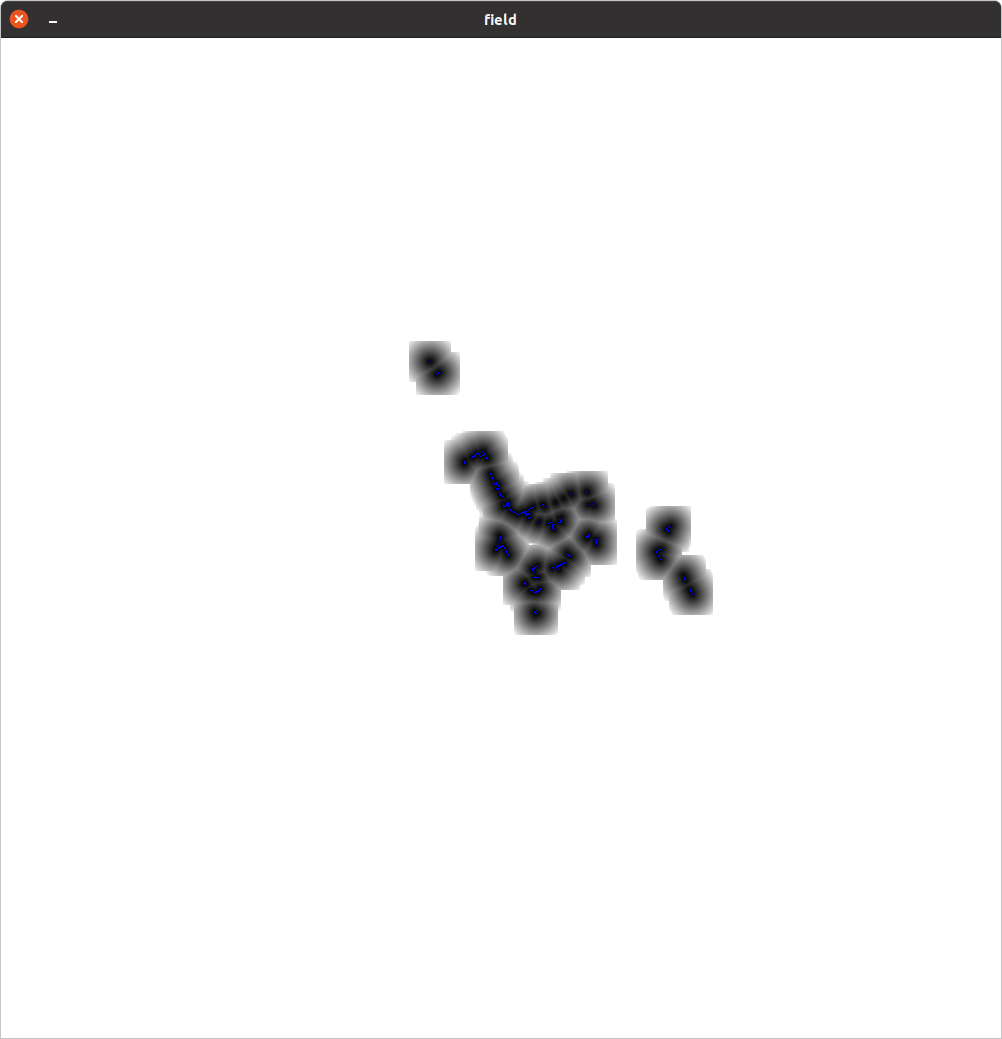
\includegraphics[width=0.5\textwidth]{resources/2d-lidar-mapping/likelihood-field}
	\caption{An example of a likelihood field}
	\label{fig:likelihood-field}
\end{figure}

Figure~\ref{fig:likelihood-field} shows a 2D scan dataset and its corresponding likelihood field. Visually, we can observe that the likelihood field radiates from each scan point and gradually decays with distance. We can customize its range and decay characteristics. The likelihood field essentially describes a distance function between each pixel and its nearest scan point, also referred to as a distance transform map in some applications \cite{Felzenszwalb2012}. With the likelihood field, we no longer need nearest neighbor structures like K-d trees to find the closest point for a given point; instead, we can directly use the field's readings.

Next, we derive the scan matching algorithm based on the likelihood field. The readings from the likelihood field can directly serve as the objective function for registration. Consider a point $\mathbf{p}^B_i$ transformed by pose $\mathbf{x}$ to obtain $\mathbf{p}^W_i$ in the world coordinate frame. Simultaneously, there exists a likelihood field $\pi$ in the world coordinate frame\footnote{Note that the likelihood field doesn't necessarily need to be maintained in the world coordinate frame; later discussions will show it is primarily maintained in submap coordinates.}. The reading of this point in the likelihood field $\pi$ is $\pi(\mathbf{p}^W_i)$. Thus, $\mathbf{x}$ can be obtained by solving the optimization problem:
\begin{equation}\label{key}
	\mathbf{x}^* = \arg \min_{\mathbf{x}} \sum_{i=1}^{n} \| \pi(\mathbf{p}_i^W) \|_2^2.
\end{equation}

The Jacobian matrix of the $\pi$ function with respect to pose $\mathbf{x}$ can be decomposed via the chain rule:
\begin{equation}\label{key}
	\frac{\partial \pi}{\partial \mathbf{x}} = \frac{\partial \pi}{\partial \mathbf{p}^W_i} \frac{\partial \mathbf{p}^W_i}{\partial \mathbf{x}}.
\end{equation}
The latter term is given in Equation \eqref{eq:dpw-dx}, so we focus on the former term.

Since the likelihood field is stored as an image, $\mathbf{p}^W_i$ must be sampled at a certain resolution. Let the transformation from $\mathbf{p}^W_i$ to its image coordinates $\mathbf{p}^f_i$ be:
\begin{equation}\label{key}
	\mathbf{p}^f_i = \alpha \mathbf{p}^W_i + \mathbf{c},
\end{equation}
where $\alpha$ is the scaling factor and $\mathbf{c} \in \mathbb{R}^2$ is the offset of the image center. Note that image coordinates typically start from the top-left corner, while object coordinates usually originate from the center, so the offset is typically half the image dimensions. The derivative of function $\pi$ with respect to $\mathbf{p}^W_i$ is:
\begin{equation}\label{key}
	\frac{\partial \pi}{\partial \mathbf{p}^W_i} = \frac{\partial \pi}{\partial \mathbf{p}^f_i} \frac{\partial \mathbf{p}^f_i}{\partial \mathbf{p}^W_i}= \alpha [\Delta \pi_x, \Delta \pi_y]^\top,
\end{equation}
where $[\Delta \pi_x, \Delta \pi_y]$ represents the gradient of the likelihood field in the image. Since we define the likelihood function for each point as a smooth function, its gradient is equally reliable. Multiplying these two matrices yields the Jacobian matrix of each residual with respect to the pose:
\begin{equation}\label{key}
	\frac{\partial \pi}{\partial \mathbf{x}} = [\alpha \Delta \pi_x, \alpha \Delta \pi_y, -\alpha \Delta \pi_x r_i \sin(\rho_i+\theta) + \alpha \Delta \pi_y r_i \cos(\rho_i +\theta)]^\top.
\end{equation}

Using this Jacobian matrix, we can implement registration based on the Gauss-Newton method.

\subsection{Implementation of Likelihood Field Method (Gauss-Newton)}  

When implementing the likelihood field method, we need to generate the corresponding likelihood field when setting the target point cloud. Each point in the likelihood field can use a pre-generated, fixed-size template, which is then "pasted" onto each point of the target point cloud.  

\begin{lstlisting}[language=c++,caption=src/ch6/likelihood\_field.cc]  
class LikelihoodField {  
	public:  
	/// 2D field template, generated when setting target scan or map  
	struct ModelPoint {  
		ModelPoint(int dx, int dy, float res) : dx_(dx), dy_(dy), residual_(res) {}  
		int dx_ = 0;  
		int dy_ = 0;  
		float residual_ = 0;  
	};  
	
	private:  
	std::vector<ModelPoint> model_;  // 2D template  
};  

void LikelihoodField::BuildModel() {  
	const int range = 20;  // Template size in pixels  
	for (int x = -range; x <= range; ++x) {  
		for (int y = -range; y <= range; ++y) {  
			model_.emplace_back(x, y, std::sqrt((x * x) + (y * y)));  
		}  
	}  
}  

void LikelihoodField::SetTargetScan(Scan2d::Ptr scan) {  
	target_ = scan;  
	
	// Generate field function on target points  
	field_ = cv::Mat(1000, 1000, CV_32F, 30.0);  
	
	for (size_t i = 0; i < scan->ranges.size(); ++i) {  
		if (scan->ranges[i] < scan->range_min || scan->ranges[i] > scan->range_max) {  
			continue;  
		}  
		
		double real_angle = scan->angle_min + i * scan->angle_increment;  
		double x = scan->ranges[i] * std::cos(real_angle) * resolution_ + 500;  
		double y = scan->ranges[i] * std::sin(real_angle) * resolution_ + 500;  
		
		// Fill field function around (x,y)  
		for (auto& model_pt : model_) {  
			int xx = int(x + model_pt.dx_);  
			int yy = int(y + model_pt.dy_);  
			if (xx >= 0 && xx < field_.cols && yy >= 0 && yy < field_.rows &&  
			field_.at<float>(yy, xx) > model_pt.residual_) {  
				field_.at<float>(yy, xx) = model_pt.residual_;  
			}  
		}  
	}  
}  
\end{lstlisting}  

We use a 1000$\times$1000 pixel image to store the likelihood field data. This class generates a template with a 20-pixel edge length during construction and then applies this template to each point.  

Once the likelihood field is generated, we can use the previously described Gauss-Newton iteration method to register two scan datasets.  

\begin{lstlisting}[language=c++,caption=src/ch6/likelihood\_field.cc]  
bool LikelihoodField::AlignGaussNewton(SE2& init_pose) {  
	int iterations = 10;  
	double cost = 0, lastCost = 0;  
	SE2 current_pose = init_pose;  
	const int min_effect_pts = 20;  // Minimum number of effective points  
	const int image_boarder = 20;   // Image border margin  
	
	for (int iter = 0; iter < iterations; ++iter) {  
		Mat3d H = Mat3d::Zero();  
		Vec3d b = Vec3d::Zero();  
		cost = 0;  
		
		int effective_num = 0;  // Number of effective points  
		
		// Traverse source points  
		for (size_t i = 0; i < source_->ranges.size(); ++i) {  
			float r = source_->ranges[i];  
			if (r < source_->range_min || r > source_->range_max) {  
				continue;  
			}  
			
			float angle = source_->angle_min + i * source_->angle_increment;  
			float theta = current_pose.so2().log();  
			Vec2d pw = current_pose * Vec2d(r * std::cos(angle), r * std::sin(angle));  
			
			// Image coordinates in the field  
			Vec2i pf = (pw * resolution_ + Vec2d(500, 500)).cast<int>();  
			
			if (pf[0] >= image_boarder && pf[0] < field_.cols - image_boarder && pf[1] >= image_boarder &&  
			pf[1] < field_.rows - image_boarder) {  
				effective_num++;  
				
				// Image gradient  
				float dx = 0.5 * (field_.at<float>(pf[1], pf[0] + 1) - field_.at<float>(pf[1], pf[0] - 1));  
				float dy = 0.5 * (field_.at<float>(pf[1] + 1, pf[0]) - field_.at<float>(pf[1] - 1, pf[0]));  
				
				Vec3d J;  
				J << resolution_ * dx, resolution_ * dy,  
				-resolution_ * dx * r * std::sin(angle + theta) + resolution_ * dy * r * std::cos(angle + theta);  
				H += J * J.transpose();  
				
				float e = field_.at<float>(pf[1], pf[0]);  
				b += -J * e;  
				
				cost += e * e;  
			}  
		}  
		
		if (effective_num < min_effect_pts) {  
			return false;  
		}  
		
		// solve for dx  
		Vec3d dx = H.ldlt().solve(b);  
		if (isnan(dx[0])) {  
			break;  
		}  
		
		cost /= effective_num;  
		if (iter > 0 && cost >= lastCost) {  
			break;  
		}  
		
		LOG(INFO) << "iter " << iter << " cost = " << cost << ", effect num: " << effective_num;  
		
		current_pose.translation() += dx.head<2>();  
		current_pose.so2() = current_pose.so2() * SO2::exp(dx[2]);  
		lastCost = cost;  
	}  
	
	init_pose = current_pose;  
	return true;  
}  
\end{lstlisting}  

We only need to replace the residuals and Jacobians from the previous ICP with those from the likelihood field. Readers can run the provided test program to view the matching results of the 2D likelihood field method:  

\begin{lstlisting}[language=sh,caption=Terminal input:]  
bin/test_2d_icp_likelihood   
\end{lstlisting}  

In addition to displaying the registration results, this program also shows real-time single-frame likelihood field data. Readers should observe that the likelihood field aligns with the scan data, as shown in Figure~\ref{fig:scan-and-field}.  

\begin{figure}[!htp]  
	\centering  
	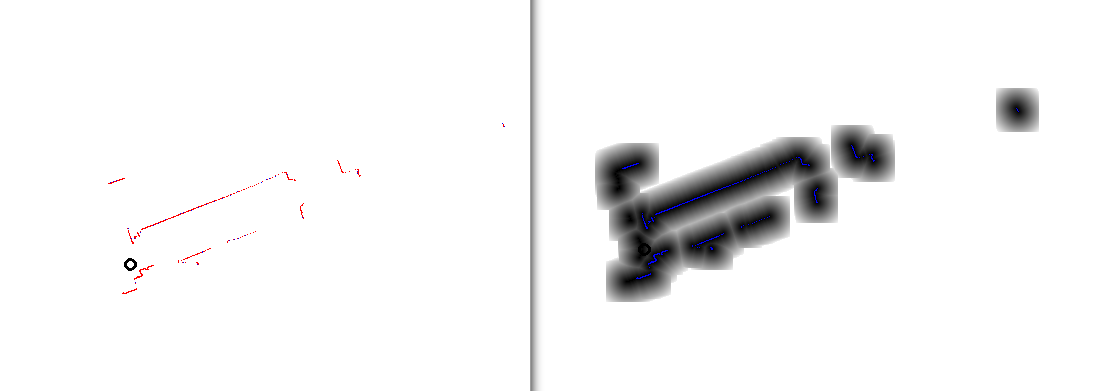
\includegraphics[width=0.8\textwidth]{resources/2d-lidar-mapping/ch6-scan-and-filed.png}  
	\caption{Real-time scan data and likelihood field data}  
	\label{fig:scan-and-field}  
\end{figure}

\subsection{Implementation of Likelihood Field Method (g2o)}
Below we demonstrate how to use the g2o optimizer \cite{Kummerle2011} to implement a likelihood field-based scan matching algorithm. By using an optimizer, we can more conveniently employ different iteration strategies and set robust kernel functions to achieve more robust matching algorithms. In fact, all the registration methods implemented earlier can be adapted to an optimizer-based approach. Now we define the $\mathrm{SE}(2)$ pose vertex and the observation error edges corresponding to each scan point.

\begin{lstlisting}[language=c++,caption=src/ch6/g2o\_types.h]
class VertexSE2 : public g2o::BaseVertex<3, SE2> {
	public:
	EIGEN_MAKE_ALIGNED_OPERATOR_NEW
	
	void setToOriginImpl() override { _estimate = SE2(); }
	void oplusImpl(const double* update) override {
		_estimate.translation()[0] += update[0];
		_estimate.translation()[1] += update[1];
		_estimate.so2() = _estimate.so2() * SO2::exp(update[2]);
	}
};

class EdgeSE2LikelihoodFiled : public g2o::BaseUnaryEdge<1, double, VertexSE2> {
	public:
	EIGEN_MAKE_ALIGNED_OPERATOR_NEW;
	EdgeSE2LikelihoodFiled(const cv::Mat& field_image, double range, double angle, float resolution 
	= 10.0) : field_image_(field_image), range_(range), angle_(angle), resolution_(resolution) {}
	
	void computeError() override {
		VertexSE2* v = (VertexSE2*)_vertices[0];
		SE2 pose = v->estimate();
		Vec2d pw = pose * Vec2d(range_ * std::cos(angle_), range_ * std::sin(angle_));
		Vec2i pf = (pw * resolution_ + Vec2d(field_image_.rows / 2, field_image_.cols / 2)).cast<int>(); 
		
		if (pf[0] >= image_boarder_ && pf[0] < field_image_.cols - image_boarder_ && pf[1] >= 
		image_boarder_ && pf[1] < field_image_.rows - image_boarder_) {
			_error[0] = field_image_.at<float>(pf[1], pf[0]);
		} else {
			_error[0] = 0;
			setLevel(1);
		}
	}
	
	void linearizeOplus() override {
		VertexSE2* v = (VertexSE2*)_vertices[0];
		SE2 pose = v->estimate();
		float theta = pose.so2().log();
		Vec2d pw = pose * Vec2d(range_ * std::cos(angle_), range_ * std::sin(angle_));
		Vec2i pf = (pw * resolution_ + Vec2d(field_image_.rows / 2, field_image_.cols / 2)).cast<int>();
		
		if (pf[0] >= image_boarder_ && pf[0] < field_image_.cols - image_boarder_ && pf[1] >= 
		image_boarder_ && pf[1] < field_image_.rows - image_boarder_) {
			// Image gradient
			float dx = 0.5 * (field_image_.at<float>(pf[1], pf[0] + 1) - field_image_.at<float>(pf[1], pf[0] - 1));
			float dy = 0.5 * (field_image_.at<float>(pf[1] + 1, pf[0]) - field_image_.at<float>(pf[1] - 1, pf[0]));
			
			_jacobianOplusXi << resolution_ * dx, resolution_ * dy,
			-resolution_ * dx * range_ * std::sin(angle_ + theta) +
			resolution_ * dy * range_ * std::cos(angle_ + theta);
		} else {
			_jacobianOplusXi.setZero();
			setLevel(1);
		}
	}
	
	private:
	const cv::Mat& field_image_;
	double range_;
	double angle_;
	float resolution_ = 10.0;
	inline static const int image_boarder_ = 10;
};
\end{lstlisting}

The Jacobian matrix here is consistent with our previous derivation, except that the likelihood field image has been moved inside the class for quick lookup of corresponding field function values and their gradients. Next, we only need to convert the iteration process from the Gauss-Newton method into an optimization problem.

\begin{lstlisting}[language=c++,caption=src/ch6/likelihood\_field.cc]
bool LikelihoodField::AlignG2O(SE2& init_pose) {
	using BlockSolverType = g2o::BlockSolver<g2o::BlockSolverTraits<3, 1>>;
	using LinearSolverType = g2o::LinearSolverCholmod<BlockSolverType::PoseMatrixType>;
	auto* solver = new g2o::OptimizationAlgorithmLevenberg(
	g2o::make_unique<BlockSolverType>(g2o::make_unique<LinearSolverType>()));
	g2o::SparseOptimizer optimizer;
	optimizer.setAlgorithm(solver);
	
	auto* v = new VertexSE2();
	v->setId(0);
	v->setEstimate(init_pose);
	optimizer.addVertex(v);
	
	// Traverse source points
	for (size_t i = 0; i < source_->ranges.size(); ++i) {
		float r = source_->ranges[i];
		if (r < source_->range_min || r > source_->range_max) {
			continue;
		}
		
		float angle = source_->angle_min + i * source_->angle_increment;
		auto e = new EdgeSE2LikelihoodFiled(field_, r, angle, resolution_);
		e->setVertex(0, v);
		e->setInformation(Eigen::Matrix<double, 1, 1>::Identity());
		optimizer.addEdge(e);
	}
	
	optimizer.setVerbose(true);
	optimizer.initializeOptimization();
	optimizer.optimize(10);
	
	init_pose = v->estimate();
	return true;
}
\end{lstlisting}

This implements the g2o-based 2D scan matching algorithm. By adding --method=g2o to the test program in Section~\ref{sec:likelihood-field}, you can test the optimizer version of likelihood field matching. Since the results are similar, we won't include result images in this section. Readers can also implement versions based on Ceres or other optimizers following similar principles. Additionally, we can perform linear interpolation on the likelihood field image (Figure~\ref{fig:scan-and-field}) to obtain more accurate error functions. We leave these two aspects as exercises.

\section{Occupancy Grid Map}  
\subsection{Principle of Occupancy Grid Map}  
After performing scan matching, we obtain the relative motion between two sets of scan data. This process is equivalent to the \textbf{localization} problem in SLAM. Now, let us examine the \textbf{mapping} component.  

If we use the scan-to-map approach for scan matching, we can derive its pose relative to the map. Naturally, we can merge this scan data into the map to form a local map. However, there are some considerations in the actual map-building process. For example, should the map be constructed all at once or piece by piece? Should all scan points be combined into a single map, or should strategies like overlapping and refreshing be implemented? Early 2D SLAM solutions often adopted a simpler, monolithic map-building approach, but this method has many limitations. Therefore, this book introduces a more flexible management model based on \textbf{grid maps} and \textbf{submaps}.  

First, let us discuss the \textbf{occupancy grid map}. An occupancy grid is a map format that stores occupancy probabilities in a grid-like (or image-like) structure. A grid is a very simple form of a 2D map. It divides the map into many small planar cells, each storing custom information. The organization of this information is highly flexible. If obstacle information is stored, it is called an obstacle grid map, which can be used for path planning \cite{Tsardoulias2016}. In some applications, semantic information is also stored in grids, known as semantic grids \cite{Qi2020}. Grid maps are often associated with images, where each grid cell corresponds to a pixel. The storage and visualization of grid maps can be implemented using image libraries like OpenCV. Overall, grid maps are a widely used method for representing dense information on a 2D plane.  

In many robotic applications, people are only concerned with the \textbf{traversability} of each grid cell and not more complex semantic information (though passenger vehicles are an exception, which is why grid maps are rarely used in outdoor vehicles). Therefore, we only need to indicate whether a grid cell is occupied by an obstacle. The presence of an obstacle is probabilistic. Before scanning the map, we have no knowledge of whether obstacles exist, so the occupancy probability should initially be set to 0.5. If a grid cell is observed multiple times to contain an obstacle, its occupancy probability gradually increases to 1. Conversely, if a grid cell is repeatedly observed to be traversable, its probability decreases to 0. The endpoint measured by a 2D laser sensor indicates that the grid is occupied, while the line connecting the sensor to the endpoint indicates that the grid is traversable. Thus, 2D laser scan data can be easily converted into a grid format.  

It is worth noting that some applications use \textbf{occupancy} grids to represent obstacles, while others use \textbf{traversability} probability to indicate whether a grid is passable. These two probabilities are inversely related but functionally equivalent. In an occupancy grid, a probability of 1 means the grid contains an obstacle, whereas in a traversability grid, a probability of 1 means the grid is obstacle-free. In practice, both approaches can be used freely.  

On the other hand, grid maps can be dynamically updated, and not every grid cell's probability converges to 0 or 1. If a robot observes a grid cell as an obstacle multiple times, its occupancy probability will continuously rise. If a cell is repeatedly observed as empty, its occupancy probability should decrease. If an obstacle initially exists but later moves away, the grid cell's probability will first increase and then decrease. In summary, an occupancy grid map should satisfy the following descriptions:  

\begin{enumerate}  
	\item It stores the probability of each grid cell being occupied by an obstacle in a grid-like format. This probability should be a floating-point number between 0 and 1.  
	\item The grid has a certain resolution and is typically dense.  
	\item The occupancy probability changes with observations. Mathematically, the update logic for occupancy probability should comply with probabilistic principles. However, from an engineering perspective, simpler metrics like observation counts can also be used.  
\end{enumerate}  

\begin{figure}[!htp]  
	\centering  
	\includegraphics[width=0.8\textwidth]{resources/2d-lidar-mapping/grid-and-casting.pdf}  
	\caption{Occupancy grid and ray casting process for 2D LiDAR}  
	\label{fig:grid-and-casting}  
\end{figure}  

Figure~\ref{fig:grid-and-casting}~shows an example of a 2D LiDAR scan being converted into grid cells. When a laser beam is emitted from the sensor, the endpoint corresponds to an occupied grid cell, while the path from the sensor center to the endpoint is considered traversable. Note that this geometric model is only valid for \textbf{2D} robots. If the robot has significant height or the laser beams are tilted, this model no longer applies. In such cases, the 2D LiDAR occupancy grid can only indicate whether obstacles exist \textbf{at this specific height}. Obstacles at other heights, such as low steps, tables, or hanging objects, may still render the robot unable to pass. Therefore, if the robot's motion cannot be simplified to 2D, the map must account for the influence of obstacles at other heights.  

Due to the resolution limitations of grid maps, converting continuous laser beams into probability updates for each grid cell involves a \textbf{rasterization} process, as illustrated on the right side of Figure~\ref{fig:grid-and-casting}~. Rasterization is a concept in computer graphics that describes the conversion of geometric shapes into grid-based outputs. In 2D grid maps, we can choose to compute the rasterization result for each laser beam. However, if the LiDAR's angular resolution is high or the measurement range is long, this process can be time-consuming. Alternatively, we can precompute a fixed-size template region. The former requires rasterizing each laser scan line, while the latter involves rasterizing each template point. We will implement both algorithms and compare their performance.

\subsection{Map Generation Based on Bresenham's Algorithm}  
Bresenham's algorithm is a rasterization method for straight lines, commonly used for vectorization of geometric lines \cite{Cohen-Or1997}. It can be implemented entirely with integer operations, making it highly efficient. Since grid map coordinates are inherently integer-based, Bresenham's algorithm is well-suited for updating grid maps.  

Let the robot's origin in the map coordinate system be $\mathbf{p}_1$, and an endpoint be $\mathbf{p}_2$, both with integer coordinates. We aim to fill a straight line from $\mathbf{p}_1$ to $\mathbf{p}_2$ in the map, marking these cells as traversable. The Bresenham algorithm proceeds as follows:  

\begin{enumerate}  
	\item Compute $[dx, dy] = p2 - p1$, representing the direction of coordinate growth.  
	\item Compare $|dx|$ and $|dy|$, selecting the larger one as the primary growth axis (assume the $x$-axis for now).  
	\item Initialize $(x, y)$ at $\mathbf{p}_1$. Since the line's slope is $dy/dx$, each time $x$ increments by 1, the error between the discrete point and the true line increases by $dy/dx$. When this error exceeds 0.5, increment $y$ by 1 and decrease the error by 1.  
	\item Repeat until $(x, y)$ reaches $\mathbf{p}_2$.  
\end{enumerate}  

Step 3 involves floating-point operations, but we prefer integer-only computation. Thus, we multiply all terms and conditions in Step 3 by $2dx$ and subtract $dx$, transforming it into:  

\begin{enumerate}  
	\item Compute $[dx, dy] = p2 - p1$, representing the direction of coordinate growth.  
	\item Compare $|dx|$ and $|dy|$, selecting the larger one as the primary growth axis (assume the $x$-axis for now).  
	\item Initialize $(x, y)$ at $\mathbf{p}_1$ and set the initial error $e = -dx$. Each time $x$ increments by 1, $e$ increases by $2dy$. If $e > 0$, increment $y$ by 1 and subtract $2dx$ from $e$.  
	\item Repeat until $(x, y)$ reaches $\mathbf{p}_2$.  
\end{enumerate}  

This avoids floating-point and division operations, using only additions and multiplications. Similarly, if the $y$-axis is the primary growth direction, swap the roles of $x$ and $y$.  

The implementation of Bresenham's algorithm in the grid map is as follows:  

\begin{lstlisting}[language=c++,caption=src/ch6/occupancy\_map.cc]  
void OccupancyMap::BresenhamFilling(const Vec2i& p1, const Vec2i& p2) {  
	int dx = p2.x() - p1.x();  
	int dy = p2.y() - p1.y();  
	int ux = dx > 0 ? 1 : -1;  
	int uy = dy > 0 ? 1 : -1;  
	
	dx = abs(dx);  
	dy = abs(dy);  
	int x = p1.x();  
	int y = p1.y();  
	
	if (dx > dy) {  
		// Increment along x  
		int e = -dx;  
		for (int i = 0; i < dx; ++i) {  
			x += ux;  
			e += 2 * dy;  
			if (e >= 0) {  
				y += uy;  
				e -= 2 * dx;  
			}  
			
			if (Vec2i(x, y) != p2) {  
				SetPoint(Vec2i(x, y), false);  
			}  
		}  
	} else {  
		int e = -dy;  
		for (int i = 0; i < dy; ++i) {  
			y += uy;  
			e += 2 * dx;  
			if (e >= 0) {  
				x += ux;  
				e -= 2 * dy;  
			}  
			if (Vec2i(x, y) != p2) {  
				SetPoint(Vec2i(x, y), false);  
			}  
		}  
	}  
}  

/// Set whether a grid cell is occupied  
void OccupancyMap::SetPoint(const Vec2i& pt, bool occupy) {  
	int x = pt[0], y = pt[1];  
	if (x < 0 || y < 0 || x >= occupancy_grid_.cols || y >= occupancy_grid_.rows) {  
		if (occupy) {  
			has_outside_pts_ = true;  
		}  
		return;  
	}  
	
	/// Apply upper and lower bounds  
	uchar value = occupancy_grid_.at<uchar>(y, x);  
	if (occupy) {  
		if (value > 117) {  
			occupancy_grid_.ptr<uchar>(y)[x] -= 1;  
		}  
	} else {  
		if (value < 137) {  
			occupancy_grid_.ptr<uchar>(y)[x] += 1;  
		}  
	}  
}  
\end{lstlisting}

Now, readers are invited to compile and run the `test_occupancy_grid` program:
\begin{lstlisting}[language=sh,caption=Terminal input:]
	bin/test_occupancy_grid --bag_path ./dataset/sad/2dmapping/floor1.bag 
\end{lstlisting}

You can specify different filling methods using the `--method` option. The program will display the grid map results generated from a single scan, as shown in Figure~\ref{fig:oc-grid-one-scan}~. The final grid map is the superposition of these individual grid maps. As can be observed, the obstacles and traversable areas obtained from 2D LiDAR scans match our intuitive expectations.

The LiDAR used in our experiments does not have 360-degree coverage, leaving a blind spot behind the robot. For most robots with substantial height, it's impossible to completely suspend sensors in midair, inevitably causing partial occlusion of sensor data.

In this chapter's test program, we can observe that the template-based algorithm requires approximately 10-20ms to complete template filling, while the line-based method takes less than 1 millisecond - a significant difference. This is because the template method processes significantly more points than the line method (hundreds of thousands versus hundreds). If the LiDAR's angular resolution increases or the detection range extends, the template method can limit its computation range to save processing time.

\begin{figure}[!t]
	\centering
	\includegraphics[width=0.4\textwidth]{resources/2d-lidar-mapping/oc-grid-one-scan.png}
	\caption{Grid map generated from a single scan}
	\label{fig:oc-grid-one-scan}
\end{figure}

In template-based grid map updating, the sizes of submaps and templates should be set according to the actual sensor range. If the template is too small, distant scan data may not be fully utilized; if submap size is insufficient, frequent submap expansion may occur, introducing unnecessary computations. Here we've used parameters suitable for a 20m LiDAR range, with both grid template and submap sizes configured accordingly. For readers using longer-range LiDARs, these parameters should be appropriately increased. Note that algorithm efficiency will change noticeably with parameter adjustments - readers are encouraged to experiment with different settings.

\section{Submaps}  
\subsection{Principle of Submaps}  
Next, we integrate the matching algorithm with grid maps, utilizing the grid map update mechanism to combine matched data.  

Furthermore, we can group several matched results together to form \textbf{submaps}. Submaps serve as an intermediate data organization level between individual scan data and the global map. They flexibly aggregate multiple scans in chronological order and can be used in both 2D LiDAR SLAM and 3D LiDAR SLAM systems.  

Each submap is assigned an adjustable pose denoted by $\mathbf{T}_{WS} \in \mathrm{SE}(2)$, where $W$ represents the world coordinate system and $S$ represents the submap coordinate system. During scan matching, the scan-to-map algorithm essentially computes the pose relationship $\mathbf{T}_{SC}$ between the current LiDAR scan and the submap, where $C$ denotes the current scan coordinate system. Thus, the world coordinate of each scan can be expressed as:  
\begin{equation}\label{key}  
\mathbf{T}_{WC} = \mathbf{T}_{WS} \mathbf{T}_{SC}.  
\end{equation}  

This approach decouples the \textbf{submap pose} variable $\mathbf{T}_{WS}$. During scan matching, we compute $\mathbf{T}_{SC}$ for the current LiDAR scan, which remains fixed once determined. When adjusting the overall map shape, we only need to modify each submap's $\mathbf{T}_{WS}$ without altering internal submap contents (i.e., per-scan $\mathbf{T}_{SC}$). Consequently, loop closure detection can treat submaps as fundamental units without considering individual keyframe poses in the world coordinate system.  

We implement a submap-based 2D LiDAR SLAM system following this logic:  
\begin{enumerate}  
	\item Each submap is associated with a likelihood field and a grid map.  
	\item The current scan is always matched against the current submap to determine its pose within the submap\footnote{This step is flexible in implementation. With sufficient computational resources, matching against historical submaps is also feasible.}.  
	\item Keyframes are selected based on travel distance or rotation thresholds.  
	\item If the robot moves beyond the current submap's bounds or the submap contains excessive keyframes, a new submap is created. The new submap centers on the current frame with $\mathbf{T}_{WS} = \mathbf{T}_{WC}$, initially empty. For matching convenience, recent keyframes from the old submap are copied to the new one.  
	\item Merging all submaps' grid maps yields the global map.  
\end{enumerate}  

This workflow is not limited to 2D LiDAR SLAM. The submap paradigm can also be applied to 3D LiDAR or visual SLAM systems, though implementation becomes more complex than single-map approaches.

\subsection{Implementation of Submaps}  
At the implementation level, we encapsulate both grid map and likelihood field objects within the `Submap` class, while placing the mapping algorithm workflow in the `mapping_2d` class.  

The core structure of the `Submap` class is as follows:  
\begin{lstlisting}[language=c++,caption=src/ch6/submap.h]
class Submap {
	public:
	Submap(const SE2& pose) : pose_(pose) {
		Vec2f center = pose_.translation().cast<float>();
		occu_map_.SetCenter(center);
		field_.SetCenter(center);
	}
	
	/// Match frame against this submap to compute frame->pose
	bool MatchScan(std::shared_ptr<Frame> frame);
	
	/// Add a frame to the occupancy grid
	void AddScanInOccupancyMap(std::shared_ptr<Frame> frame);
	
	void AddKeyFrame(std::shared_ptr<Frame> frame) { frames_.emplace_back(frame); }
	
	private:
	SE2 pose_;  // submap pose, Tws
	size_t id_ = 0;
	
	std::vector<std::shared_ptr<Frame>> frames_;  // keyframes in this submap
	LikelihoodField field_;                       // for scan matching
	OccupancyMap occu_map_;                       // for grid map generation
};
\end{lstlisting}

The submap's primary functions are scan matching and grid map updates, implemented through internal object calls:  

\begin{lstlisting}[language=c++,caption=src/ch6/submap.cc]
bool Submap::MatchScan(std::shared_ptr<Frame> frame) {
	field_.SetSourceScan(frame->scan_);
	field_.AlignG2O(frame->pose_submap_);
	frame->pose_ = pose_ * frame->pose_submap_;  // T_w_c = T_w_s * T_s_c
	
	return true;
}

void Submap::AddScanInOccupancyMap(std::shared_ptr<Frame> frame) {
	occu_map_.AddLidarFrame(frame, OccupancyMap::GridMethod::MODEL_POINTS);  // update grid cells
	field_.SetFieldImageFromOccuMap(occu_map_.GetOccupancyGrid());           // update likelihood field
}
\end{lstlisting}

We employ g2o-based likelihood field methods for registration, incorporating boundary checks and robust kernels to mitigate moving object interference. Readers may refer to the source code for implementation details. The outer mapping workflow proceeds as follows:  

\begin{lstlisting}[language=c++,caption=src/ch6/mapping\_2d.cc]
bool Mapping2D::ProcessScan(Scan2d::Ptr scan) {
	current_frame_ = std::make_shared<Frame>(scan);
	current_frame_->id_ = frame_id_++;
	
	LOG(INFO) << "processing frame " << current_frame_->id_;
	if (last_frame_) {
		// initialize pose from last frame
		current_frame_->pose_ = last_frame_->pose_;
	}
	
	// perform scan-to-map matching
	if (!first_scan_) {
		// skip matching for first scan (directly add to occupancy map)
		current_submap_->MatchScan(current_frame_);
	}
	
	first_scan_ = false;
	current_submap_->AddScanInOccupancyMap(current_frame_);
	
	if (IsKeyFrame()) {
		AddKeyFrame();
		
		if (current_submap_->HasOutsidePoints() || (current_submap_->NumFrames()) > 50) {
			/// Trigger new submap when leaving current bounds or exceeding keyframe limit
			ExpandSubmap();
		}
	}
	
	last_frame_ = current_frame_;
	
	return true;
}

bool Mapping2D::IsKeyFrame() {
	if (last_keyframe_ == nullptr) {
		return true;
	}
	
	SE2 delta_pose = last_keyframe_->pose_.inverse() * current_frame_->pose_;
	if (delta_pose.translation().norm() > keyframe_pos_th_ || 
	fabs(delta_pose.so2().log()) > keyframe_ang_th_) {
		return true;
	}
	
	return false;
}

void Mapping2D::AddKeyFrame() {
	LOG(INFO) << "add keyframe " << keyframe_id_;
	current_frame_->keyframe_id_ = keyframe_id_++;
	
	current_submap_->AddKeyFrame(current_frame_);
	last_keyframe_ = current_frame_;
}

void Mapping2D::ExpandSubmap() {
	// archive current submap and create new one
	all_submaps_.emplace_back(current_submap_);
	
	current_submap_ = std::make_shared<Submap>(current_frame_->pose_);
	current_submap_->SetId(submap_id_++);
	current_submap_->AddKeyFrame(current_frame_);
	current_submap_->AddScanInOccupancyMap(current_frame_);
	
	LOG(INFO) << "create submap " << current_submap_->GetId();
}
\end{lstlisting}

The system continuously matches current scans against the active submap. When the robot moves beyond threshold distances, new keyframes are created and added to the current submap. Excessive keyframes trigger new submap creation, with old submaps archived for global mapping.

The test program for this section only needs to read LiDAR data from ROS bags, requiring no additional inputs. This completes our pure LiDAR-based 2D SLAM system:
\begin{lstlisting}[language=c++,caption=src/ch6/test_2d_mapping.cc]
	sad::RosbagIO rosbag_io(fLS::FLAGS_bag_path);
	sad::Mapping2D mapping;
	
	if (mapping.Init(FLAGS_with_loop_closing) == false) {
		return -1;
	}
	
	rosbag_io.AddScan2DHandle("/pavo_scan_bottom", [&](Scan2d::Ptr scan) { return mapping.ProcessScan(scan); }).Go();
	cv::imwrite("./data/ch6/global_map.png", mapping.ShowGlobalMap(1000));
	return 0;
\end{lstlisting}

Readers can run the \texttt{test\_2d\_mapping} program to observe the submap switching process along with each submap's grid and likelihood field visualization. By default, loop closure detection is disabled in this section. The next section will use the same test program with loop closure enabled to demonstrate its effects.

\begin{figure}[!htp]
	\centering
	\includegraphics[width=0.8\textwidth]{resources/2d-lidar-mapping/submap-and-field.png}
	\caption{A single submap and its corresponding likelihood field in 2D LiDAR SLAM}
	\label{fig:submap-and-field}
\end{figure}

Figure~\ref{fig:submap-and-field}~shows an active submap and its likelihood field during operation. During testing, these visualizations update dynamically, allowing readers to observe both scan matching and submap transitions. The current LiDAR pose and scan data are overlaid in contrasting colors for clearer real-time localization and mapping visualization.

In addition to the active submap, the program outputs a global map image for debugging purposes (Figure~\ref{fig:global-map-without-loop-closing}). The actual image dimensions are configurable - readers may specify larger sizes for higher-resolution outputs. Since we haven't yet implemented loop closure, accumulated drift creates visible ghosting effects when the robot revisits areas. The next section will address this through loop detection algorithms to eliminate such cumulative errors.

\begin{figure}[!t]
	\centering
	\includegraphics[width=0.4\textwidth]{resources/2d-lidar-mapping/global-map-without-loop-closing.png}
	\caption{Global map without loop closure. When the robot returns from upper regions to the central area, noticeable ghosting appears between submaps.}
	\label{fig:global-map-without-loop-closing}
\end{figure}

\section{Loop Closure Detection and Correction}
Loop closure detection constitutes a critical component in SLAM systems. Without it, both LiDAR odometry and wheel-inertial odometry methods inevitably accumulate drift over time. The previous section's example clearly demonstrates this issue - when the robot completes a loop and returns to previously mapped areas, new submaps exhibit noticeable misalignment with historical ones. This naturally suggests that aligning current scans/submaps with historical maps and adjusting inter-submap pose relationships could effectively eliminate accumulated errors. While theoretically sound, several practical challenges emerge:

\begin{enumerate}
	\item \textbf{Detection Scope}: Which historical submaps should be examined? This defines the loop \textbf{detection} problem. Intuitively, submaps spatially proximate to current scans should undergo alignment. However, spatial relationships rely on estimated trajectories that may contain significant drift, potentially causing missed detections. Effective implementation requires approximate bounds on accumulated error magnitude.
	
	\item \textbf{Registration Methods}: Loop closure registration differs fundamentally from odometric alignment. Odometry assumes \textbf{continuous motion} with small displacements between optimizations. Loop closure initial guesses, however, depend on \textbf{accumulated error magnitude} and may deviate significantly from optimal alignments. Standard ICP and likelihood field methods suffer from strong initial value dependence. Practical solutions incorporate:
	\begin{itemize}
		\item Grid searching \cite{Scherer2013}
		\item Particle filters \cite{Stachniss2005} 
		\item Branch-and-bound (BAB) \cite{Hess2016}
		\item Image pyramids \cite{Qianhao2018}
	\end{itemize}
	Among these, branch-and-bound and pyramid approaches offer particularly robust performance with similar underlying principles.
	
	\item \textbf{Map Correction}: Upon loop detection, global pose adjustment can operate on either keyframes or submaps. Submap-based optimization benefits from significantly smaller problem dimensions (fewer submaps than keyframes), making it ideal when the frontend already employs submap management. However, submap-level correction cannot address intra-submap distortions, motivating some systems to retain keyframe-level optimization.
\end{enumerate}

\subsection{Multi-Resolution Loop Closure Detection}  
We now introduce the pyramid-based loop closure detection method, also known as \textbf{coarse-to-fine} or multi-resolution registration. Rather than being a single algorithm, this represents a general strategy for addressing initialization problems - an approach widely applicable beyond point cloud registration. For instance:  
- Branch-and-bound serves both as a coarse registration method and a fundamental technique in integer programming  
- Pyramid methods are equally vital for likelihood field registration and optical flow computation \cite{Fortun2015}  

From a search perspective, these methods efficiently explore solution spaces while maintaining optimality. Since both branch-and-bound and coarse-to-fine approaches utilize multi-resolution grid maps, we classify them collectively as multi-resolution loop closure techniques.  

This section focuses on multi-resolution likelihood field matching. While fundamentally still a scan matching problem, it specifically addresses scenarios with poor initial pose estimates. Our implementation extends the standard likelihood field (20 pixels/meter resolution) with additional lower-resolution fields. As shown in Figure~\ref{fig:multi-level-search}, we employ four field layers where each higher level halves the image dimensions. The coarsest level's blurred obstacle representations permit larger initial pose errors while maintaining discriminative power.  

\begin{figure}[!t]  
	\centering  
	\includegraphics[width=0.8\textwidth]{resources/2d-lidar-mapping/multi-level-search.png}  
	\caption{Multi-resolution registration visualization. Left: Original resolution field; Right: Downsampled fields. Red: Unaligned scans; Green: Registered scans.}  
	\label{fig:multi-level-search}  
\end{figure}  

The implementation (src/ch6/multi\_resolution\_likelihood\_field.cc) follows standard frame-to-frame matching but with adjusted parameters and multiple field layers:  

\begin{lstlisting}[language=c++,caption=src/ch6/multi_resolution_likelihood_field.cc]
	void MRLikelihoodField::BuildModel() {
		const int range = 20;  // Template pixel radius
		
		/// Pyramid field construction
		field_ = {
			cv::Mat(125, 125, CV_32F, 30.0),  // Level 0 (coarsest)
			cv::Mat(250, 250, CV_32F, 30.0),
			cv::Mat(500, 500, CV_32F, 30.0),
			cv::Mat(1000, 1000, CV_32F, 30.0), // Level 3 (finest)
		};
		
		// Template generation
		for (int x = -range; x <= range; ++x) {
			for (int y = -range; y <= range; ++y) {
				model_.emplace_back(x, y, std::sqrt((x * x) + (y * y)));
			}
		}
	}
	
	bool MRLikelihoodField::AlignG2O(SE2& init_pose) {
		num_inliers_.clear();
		inlier_ratio_.clear();
		
		// Hierarchical registration
		for (int l = 0; l < levels_; ++l) {
			if (!AlignInLevel(l, init_pose)) {
				return false;  // Abort if any level fails
			}
		}
		return true;
	}
	
	bool MRLikelihoodField::AlignInLevel(int level, SE2& init_pose) {
		// G2O optimization setup (omitted for brevity)
		...
		
		// Adaptive parameters
		const double rk_delta[] = {0.2, 0.3, 0.6, 0.8}; // Robust kernel thresholds
		const float inlier_ratio_th = 0.4;  // Minimum inlier percentage
		
		// Edge construction and optimization
		...
		
		// Validation
		if (num_inliers > 100 && inlier_ratio > inlier_ratio_th) {
			init_pose = v->estimate();
			return true;
		}
		return false;
	}
\end{lstlisting}

The pyramid matching proceeds sequentially - failure at any level terminates the process. Notably, loop closure scenarios often exhibit partial matches due to:  

\begin{enumerate}
\item  Significant initial pose errors  
\item  Limited LiDAR FOV (270° in our experiments)  
\item  Non-identical revisit poses 
\end{enumerate}
 

We therefore set a conservative inlier threshold (40\%) to balance sensitivity and robustness. This critical parameter trades off between:  
- \textbf{Strictness}: Higher thresholds require precise pose recurrence  
- \textbf{Sensitivity}: Lower thresholds permit more detections but increase false positives  

While we demonstrate coarse-to-fine registration, other methods like branch-and-bound \cite{Hess2016} similarly leverage multi-resolution maps. Both approaches share core principles but differ in implementation details - the former performs full optimization at each level, while the latter evaluates discrete candidates. Given their conceptual similarity, we focus on one representative implementation.

\subsection{Submap-Based Loop Closure Correction}  
If loop closure detection successfully establishes the registration relationship between the current frame and a historical submap, we initiate a loop closure correction. This problem can again be modeled as a pose graph problem on $\mathrm{SE}(2)$. Moreover, since we have already constructed submaps earlier, the pose graph problem can utilize only submap poses as optimization nodes.

Consider the relationship between the current frame and a historical submap. We compute the pose of the current frame within the historical submap through multi-resolution matching. Let the pose of the historical submap $S_1$ itself be $\mathbf{T}_{W S_1}$, the pose of the current frame be $\mathbf{T}_{WC}$, and the pose of the submap $S_2$ containing the current frame be $\mathbf{T}_{W S_2}$. The multi-resolution matching actually computes the relative pose $\mathbf{T}_{S_1 C}$. Thus, we can convert this result into the pose transformation between the historical submap and the current submap:

\begin{equation}\label{key}
	\mathbf{T}_{S_1 S_2} = \mathbf{T}_{S_1 C} \mathbf{T}_{WC}^{-1} \mathbf{T}_{W S_2}
\end{equation}
Thereby obtaining the relative pose relationship between $S_1$ and $S_2$. This process is illustrated in Figure~\ref{fig:submap-pose-graph}.

\begin{figure}[!htp]
	\centering
	\includegraphics[width=0.5\textwidth]{resources/2d-lidar-mapping/submap-pose-graph.pdf}
	\caption{Schematic diagram of submap pose graph optimization.}
	\label{fig:submap-pose-graph}
\end{figure}

In loop closure optimization, we treat each submap pose as an optimization variable and construct a pose graph for optimization. The observations in this pose graph primarily come from two sources: first, the relative pose observations between adjacent submaps, and second, the relative pose relationships between two submaps computed by loop closure detection. Again considering the relative pose between submap 1 and submap 2, assuming the relative pose observation computed by loop closure detection is $\mathbf{T}_{S_1 S_2}$, its residual term is:
\begin{equation}\label{key}
	\mathbf{e} = \mathrm{Log}( \mathbf{T}_{W S_1}^{-1} \mathbf{T}_{W S_2} \mathbf{T}_{S_1 S_2}^{-1}) \in \mathbb{R}^3.
\end{equation}

Its Jacobian matrix is rather cumbersome, so we leave it to automatic differentiation. To prevent incorrect loop closures, we also add a loop closure verification process: the accumulated error after correction should not be too large, otherwise the loop closure will be rejected as an outlier. The implementation code for loop closure detection is as follows:

\begin{lstlisting}[language=c++,caption=src/ch6/loop_closing.cc]
class LoopClosing {
	public:
	/// A loop closure constraint
	struct LoopConstraints {
		LoopConstraints(size_t id1, size_t id2, const SE2& T12) : id_submap1_(id1), id_submap2_(id2), T12_(T12) {}
		size_t id_submap1_ = 0;
		size_t id_submap2_ = 0;
		SE2 T12_;  //  Relative pose
		bool valid_ = true;
	};
	
	/// Add the most recent submap, which may still be under construction
	void AddNewSubmap(std::shared_ptr<Submap> submap);
	
	/// Add a completed submap
	void AddFinishedSubmap(std::shared_ptr<Submap> submap);
	
	/// Perform loop closure detection for a new frame and update its pose and submap poses
	void AddNewFrame(std::shared_ptr<Frame> frame);
	
	private:
	/// Detect possible loop closures between the current frame and historical maps
	bool DetectLoopCandidates();
	
	/// Match the current frame with historical submaps
	void MatchInHistorySubmaps();
	
	/// Perform pose graph optimization between submaps
	void Optimize();
	
	std::shared_ptr<Frame> current_frame_ = nullptr;
	size_t last_submap_id_ = 0;  // ID of the most recent submap
	
	std::map<size_t, std::shared_ptr<Submap>> submaps_;  // All submaps
	
	// Mapping between submaps and their multi-resolution fields
	std::map<std::shared_ptr<Submap>, std::shared_ptr<MRLikelihoodField>> submap_to_field_;
	
	std::vector<size_t> current_candidates_;                                 // Potential loop closure candidates
	std::map<std::pair<size_t, size_t>, LoopConstraints> loop_constraints_;  // Loop constraints indexed by constrained submap pairs
	
	/// Parameters
	inline static constexpr float candidate_distance_th_ = 15.0;  // Distance threshold between candidate frame and submap center
	inline static constexpr int submap_gap_ = 1;                  // Minimum submap index difference for loop closure
	inline static constexpr double loop_rk_delta_ = 1.0;          // Robust kernel threshold for loop closure
};

void LoopClosing::AddFinishedSubmap(std::shared_ptr<Submap> submap) {
	auto mr_field = std::make_shared<MRLikelihoodField>();
	mr_field->SetPose(submap->GetPose());
	mr_field->SetFieldImageFromOccuMap(submap->GetOccuMap().GetOccupancyGrid());
	submap_to_field_.emplace(submap, mr_field);
}

void LoopClosing::AddNewSubmap(std::shared_ptr<Submap> submap) {
	submaps_.emplace(submap->GetId(), submap);
	last_submap_id_ = submap->GetId();
}

void LoopClosing::AddNewFrame(std::shared_ptr<Frame> frame) {
	current_frame_ = frame;
	if (!DetectLoopCandidates()) {
		return;
	}
	
	MatchInHistorySubmaps();
	
	if (has_new_loops_) {
		Optimize();
	}
}

bool LoopClosing::DetectLoopCandidates() {
	// Require sufficient separation between current frame and historical submaps
	has_new_loops_ = false;
	if (last_submap_id_ < submap_gap_) {
		return false;
	}
	
	current_candidates_.clear();
	
	for (auto& sp : submaps_) {
		if ((last_submap_id_ - sp.first) <= submap_gap_) {
			// Skip recently created submaps
			continue;
		}
		
		// Skip if valid constraint already exists between these submaps
		auto hist_iter = loop_constraints_.find(std::pair<size_t, size_t>(sp.first, last_submap_id_));
		if (hist_iter != loop_constraints_.end() && hist_iter->second.valid_) {
			continue;
		}
		
		Vec2d center = sp.second->GetPose().translation();
		Vec2d frame_pos = current_frame_->pose_.translation();
		double dis = (center - frame_pos).norm();
		if (dis < candidate_distance_th_) {
			current_candidates_.emplace_back(sp.first);
		}
	}
	
	return !current_candidates_.empty();
}

void LoopClosing::MatchInHistorySubmaps() {
	// First save the scan, pose and submap to offline files for MR matching
	// current_frame_->Dump("./data/ch6/frame_" + std::to_string(current_frame_->id_) + ".txt");
	
	for (const size_t& can : current_candidates_) {
		auto mr = submap_to_field_.at(submaps_[can]);
		mr->SetSourceScan(current_frame_->scan_);
		
		auto submap = submaps_[can];
		SE2 pose_in_target_submap = submap->GetPose().inverse() * current_frame_->pose_;  // T_S1_C
		SE2 init_guess = pose_in_target_submap;
		
		if (mr->AlignG2O(pose_in_target_submap)) {
			// Set constraints from current submap to target submap
			// T_S1_S2 = T_S1_C * T_C_W * T_W_S2
			SE2 T_this_cur =
			pose_in_target_submap * current_frame_->pose_.inverse() * submaps_[last_submap_id_]->GetPose();
			loop_constraints_.emplace(std::pair<size_t, size_t>(can, last_submap_id_),
			LoopConstraints(can, last_submap_id_, T_this_cur));
			has_new_loops_ = true;
		}
	}
	
	current_candidates_.clear();
}
\end{lstlisting}

This code constructs a multi-resolution likelihood field for each submap upon completion, then matches recent scans with completed submaps. If multi-resolution matching succeeds, it calls the Optimize function to perform loop closure correction. The correction results directly affect each submap's pose. The Optimize function implements g2o graph optimization setup, which is similar to previously listed g2o programs and thus omitted here. To simplify the implementation, we do not run loop closure detection as a separate thread (which would require lock management for many data structures), but instead execute it sequentially in the main 2D mapping function. Meanwhile, we display submap coordinate systems and their loop closure relationships on the global map. Running the test\_2d\_mapping program with --with\_loop\_closing=true shows this process in real-time. The global map after loop closure correction is shown in Figure~\ref{fig:global-map}, where compared with the earlier Figure~\ref{fig:global-map-without-loop-closing}, clear improvements can be seen in the central section.

\begin{figure}[!t]
	\centering
	\includegraphics[width=0.5\textwidth]{resources/2d-lidar-mapping/global-map.png}
	\caption{Global map with loop closure detection and inter-submap loop constraints.}
	\label{fig:global-map}
\end{figure}

Thus, we have completed a relatively comprehensive 2D LiDAR-only SLAM program based on a submap management framework. Such grid maps can be directly used for localization and navigation if saved. Many real-world robots or functionally simple autonomous vehicles achieve self-localization and navigation through similar approaches. However, for brevity, this implementation omits many engineering details that readers may further refine.

\subsection{Discussion}  
Below we present several potential improvements to the programs in this section. As this book primarily focuses on algorithmic principles and aims to avoid excessive engineering details that could complicate the code, the following content is mainly narrative in nature.

\subsubsection{Laser Motion Compensation, Reflectivity Issues, etc.}  
First, let us examine the laser sensor itself. A laser sensor rotates periodically and is not designed to account for the simultaneous rotation of the robot's chassis. If the chassis is stationary, the laser sensor should physically rotate 360 degrees when completing a full scan. However, if the robot itself is also rotating, the actual rotation angle when the laser completes a scan may be slightly more or less than 360 degrees. This deviation depends on the speed and direction of the chassis's rotation. Similarly, translational motion of the chassis affects the actual measured distance of each laser point. This phenomenon is referred to as \textbf{motion distortion}.

\begin{figure}[!t]
	\centering
	\includegraphics[width=0.7\textwidth]{resources/2d-lidar-mapping/lidar-problems.pdf}
	\caption{Common issues in 2D LiDAR SLAM. Top-left: Without motion compensation, the laser scan covers slightly less than the actual scene; Top-right: When observing glass surfaces, perspective effects may incorrectly mark glass walls as passable areas; Bottom-left: Reflective artifacts at the end of a left wall create a phantom wall segment beyond the actual corridor; Bottom-right: Robot vibrations cause the laser to hit the ground, creating non-existent obstacles.}
	\label{fig:lidar-problems}
\end{figure}

Motion distortion can be mitigated using motion compensation algorithms. The basic idea is to acquire the robot's pose at the start and end of each laser scan cycle. Most laser sensors complete a full rotation in 100 milliseconds, so the robot's motion during this period must be accounted for by compensating each laser point. The same issue arises with 3D LiDAR sensors, which will be discussed in the next chapter. However, how do we obtain the poses at the start and end of the scan? After all, when the laser data is first received, the robot's pose has not yet been estimated, while motion compensation relies on this very estimate. In scenarios with an IMU, we can use its data to predict the robot's motion within the 100-millisecond window and thereby compensate for the distortion.

Motion compensation improves the accuracy of submap registration. We will detail the motion compensation algorithm in the chapter on 3D LiDAR SLAM (see Section~\ref{sec:motion-compensation}), as modern 3D LiDARs typically provide timestamps for each point, whereas 2D LiDARs often do not, requiring manual estimation based on the scanning process. This involves additional sensor-specific parameters, complicating the implementation.

On the other hand, LiDAR sensors measure distance based on the time difference between emitted and reflected light. If the target object absorbs, transmits, or specularly reflects the laser beam, the measured distance may be affected. A typical example is glass surfaces, which may partially reflect or transmit the laser, resulting in intermittent obstacles or walls on the map. Mirrors represent another extreme case, where the laser beam is reflected to another area, causing the measured distance in that direction to appear much longer and making the mirror itself undetectable on the map.

If the robot vibrates during motion, the LiDAR sensor may deviate from the horizontal plane, reducing measurement consistency. The laser may also hit the ground or slopes, violating the assumptions of the grid map model. Many robots require manual annotation of sloped areas in 2D SLAM. With an IMU, the robot's 3D orientation can be estimated to determine whether the laser is tilted.

The aforementioned issues can all be observed in the experiments of this section, as shown in Figure~\ref{fig:lidar-problems}. Therefore, real-world SLAM systems must address significantly more challenges than those covered in theoretical discussions.

\subsubsection{IMU and Robot Odometry Fusion}

\begin{figure}[!htp]
	\centering
	\includegraphics[width=0.7\textwidth]{resources/2d-lidar-mapping/bad-cases.pdf}
	\caption{Degeneration issues in 2D LiDAR under degenerate and open scenarios.}
	\label{fig:bad-cases}
\end{figure}

The 2D SLAM introduced in this section is a pure LiDAR solution. Although LiDAR offers high measurement accuracy, single-line LiDAR has limited observation modes and typically narrow field of view, making pure LiDAR solutions susceptible to various environmental structures. Typical examples include open areas and corridor scenarios. In these environments, 2D scan matching algorithms fundamentally cannot uniquely determine the laser scan's position, potentially exhibiting one or more additional degrees of freedom. We refer to such issues as \textbf{degeneracy problems}.

In degenerate scenarios, most pure LiDAR scan matching algorithms struggle to provide correct pose estimation. For instance, in corridor environments, likelihood field methods generate fields concentrated along both corridor walls. If the robot moves along the corridor, new scan data will appear to match perfectly with existing corridor walls. Consequently, the matching algorithm may falsely conclude the robot hasn't moved. Similar phenomena occur with ICP-type methods. Here, we say the robot's pose estimation gains \textbf{extra degrees of freedom (gauge freedom)} along the corridor direction, while the perpendicular direction remains constrained, resulting in 1 additional degree of freedom. In open square scenarios, neither translation nor rotation can be uniquely determined, yielding 3 additional degrees of freedom. Beyond corridors and squares, many regular, symmetric environments (perfect circles, single walls, multiple parallel walls, cylindrical surfaces, etc.) also exhibit degeneracy - readers should be able to identify other degenerate scenarios.

Degeneracy problems are particularly pronounced in pure LiDAR SLAM systems. Incorporating additional sensors can partially compensate for these effects. Later chapters will introduce multi-sensor fusion SLAM systems, most commonly combining IMU, wheel encoders, odometry or GPS information with LiDAR to achieve more robust performance. Both loosely-coupled and tightly-coupled approaches can compensate for LiDAR mapping or localization in degenerate scenarios.

Readers can experiment with other datasets provided in this chapter to verify the SLAM system's core functionality (see Figure~\ref{fig:other-results}). Further improvements can be achieved by implementing motion compensation, degeneracy detection, secondary echo detection, and multi-sensor fusion. However, 2D SLAM ultimately faces practical limitations and is primarily suitable for relatively simple indoor applications. The 3D SLAM introduced in the next chapter demonstrates superior performance in large-scale outdoor environments.

\begin{figure}[!t]
	\centering
	\includegraphics[width=1.0\textwidth]{resources/2d-lidar-mapping/other-results.pdf}
	\caption{Mapping results from additional datasets in this chapter.}
	\label{fig:other-results}
\end{figure}

\section{Summary}
This chapter has presented various algorithmic modules for 2D LiDAR SLAM, which historically formed the core of SLAM research. In 2D scenarios, many problems can be simplified. We implemented registration algorithms including ICP, ICL and Gaussian fields, managed them using a submap framework, and ultimately constructed global grid maps. We also explained submap management across timestamps and loop closure correction for accumulated errors. The 2D SLAM system described here serves as a prototype for various single-line LiDAR mapping and localization applications.

\section*{Exercises}
\begin{enumerate}
	\item Implement point-to-point 2D ICP using an optimization framework (based on g2o or ceres).
	\item Implement point-to-line 2D ICP using an optimization framework (based on g2o or ceres).
	\item Implement likelihood field registration method using an optimization framework (based on g2o or ceres).
	\item In the likelihood field method, interpolation of the likelihood field image can be used to obtain more accurate error values and gradient functions. Implement a likelihood field scan matching method using linear interpolation.
	\item Implement a degeneracy detection method for 2D LiDAR using line fitting.
\end{enumerate}

 
\addtocontents{toc}{\protect\setcounter{tocdepth}{2}}
\hypersetup{bookmarksdepth=2}

\appendix
\addtocontents{toc}{\protect\setcounter{tocdepth}{0}}
\hypersetup{bookmarksdepth=2}

%\input{chapters/gaussian-distribution}
%\input{chapters/matrix-derivatives}

\backmatter
\small
\bibliographystyle{ieeetr}
\bibliography{ref}
\newpage
\end{document}
